\documentclass[]{final_report}
\usepackage{graphicx}
\usepackage{hyperref}
\usepackage{titlesec}
\usepackage[utf8]{inputenc}
\usepackage[backend=biber, style=ieee]{biblatex}
\usepackage{amsmath}
\usepackage{amssymb}
\usepackage{float}
\usepackage{tabularx} % Needed for the X column type
\usepackage{booktabs} % For prettier tables
\usepackage{lipsum}   % For dummy text
\usepackage{mathtools}
\usepackage{stmaryrd}
\usepackage{mdframed}
\usepackage{caption}
\usepackage{array}
\usepackage{listings}
\usepackage[dvipsnames]{xcolor}
\usepackage{adjustbox}
\usepackage{longtable}
\usepackage{tikz}
\usepackage{rotating}
\usepackage{pdflscape}
\usepackage{fancyhdr}
\usepackage{comment}
\usepackage{multirow}
\usepackage{lscape} % Use lscape package instead of pdflscape
\usepackage{afterpage} % Required for \afterpage command
\usepackage{fancyhdr} % Required for custom headers and footers
\usepackage{everypage}





\addbibresource{fyp.bib}
\usepackage{amsthm}
\theoremstyle{definition}
\newtheorem{definition}{Definition}[chapter]
\newtheorem{basic}{Basic Definition}
\newtheorem{theorem}{Theorem}
\newtheorem{implication}{Implication}

% Define the Java code style
\lstdefinestyle{mystyle}{
    language=Java,
    commentstyle=\color{OliveGreen},
    keywordstyle=\color{blue},
    numberstyle=\tiny\color{gray},
    stringstyle=\color{red},
    basicstyle=\ttfamily\footnotesize,
    breakatwhitespace=false,         
    breaklines=true,                 
    captionpos=b,                    
    keepspaces=true,                 
    numbers=left,                    
    numbersep=5pt,                  
    showspaces=false,                
    showstringspaces=false,
    showtabs=false,                  
    tabsize=2
}
\lstset{style=mystyle}

% Define the landscape page number command
\newcommand{\Lpagenumber}{%
  \ifdim\textwidth=\linewidth
    \else
      \bgroup
      \dimendef\margin=0 %use \margin instead of \dimen0
      \ifodd\value{page}
        \margin=\oddsidemargin
      \else
        \margin=\evensidemargin
      \fi
      \raisebox{\dimexpr -\topmargin-\headheight-\headsep-0.5\linewidth}[0pt][0pt]{%
        \rlap{\hspace{\dimexpr \margin+\textheight+\footskip}%
        \llap{\rotatebox{90}{\thepage}}}}%
      \egroup
  \fi
}

% Add the page number command to every page
\AddEverypageHook{\Lpagenumber}

%%%%%%%%%%%%%%%%%%%%%%
%%% Input project details
\def\studentname{Jude Asare}
\def\reportyear{2023/2024}
\def\projecttitle{Implementing PKCS\#1 v1.5 and other deterministic RSA Signature Schemes with provably secure parameters}
\def\supervisorname{Saqib Kakvi}
\def\degree{MSci (Hons) in Computer Science (Information Security)}
\def\fullOrHalfUnit{Appendix A} 
\begin{document}


%%%%%%%%%%%%%%%%%%%%%%
%%% Table of Contents
\tableofcontents\pdfbookmark[0]{Table of Contents}{toc}\newpage



\chapter{Appendix A Software Development Methodology}
\section{Appendix A.1 Software Development Approach}
I followed the full software development lifecycle with adherence to standard software engineering principles (Test-driven Development (TDD) etc). This approach encompassed the five stages of (1) requirements specification, (2) software design that served as a blueprint for development, (3) implementation with a focus on code quality and functionality, (4) testing to guarantee software reliability and performance, and (5) documentation, for both programmers and users to enhance understanding and usability of the software.

I chose to use the Agile methodology due to its precision and adaptability which proved crucial for handling the complex cryptographic proofs at the core of signature schemes and their security. The iterative and flexible nature of Agile allowed me to constantly reassess and integrate theoretical insights into my coding, ensuring accurate implementation and prompt identification of discrepancies. In TDD, where coding was a byproduct of testing, I made sure each component functioned correctly, a critical aspect in cryptographic software where errors could have serious security consequences. This approach was particularly beneficial for the extended scope of my project (beyond PKCS#1-v1.5), which included implementing the full suite of deterministic RSA signatures. Agile's iterative sprints and milestones helped me in making accurate estimations of time and effort, preventing overruns and ensuring systematic progress. TDD complemented this by ensuring that each part of the project was thoroughly tested before moving on, which was particularly important in the integration of the multiple signature schemes.

With this, I considered each of the constituent software development phases as fluid and adaptable. The plan was not to adhere strictly to them, but rather to remain open to revisiting previous phases as necessary. I foresaw this occurring where I may have mis-estimated tasks, or received new feedback and in the end it did particularly in the second term where I greatly underestimated time it would take implement the code for the final application. 
Despite the setback I was not deterred, and the agile approach aided me in working around and managing the issue. Part of the process, involved I conducting bi-weekly meetings with my project supervisor to discuss ongoing progress, address any concerns, and define short-term objectives. Moreover, I established review reflection points which I used to regularly evaluate progress and make adjustments as needed.

*Respective TDD unit test classes can be found in the tests subdirectory of its corresponding module. All distinct features can be found in the application/modules directory. The top level application/tests directory houses integration tests.



\begin{comment}
For the development I will utilise the Agile methodology (with Test-Driven Development (TDD)) due to its suitability for projects that demand a high degree of precision and adaptability. The complexity of cryptographic proofs, central to the security of signature schemes, requires an approach that accommodates frequent reassessment and fine-tuning, which Agile provides. The theoretical aspects, particularly the cryptographic proofs, are complex and demand a deep understanding to ensure they are implemented correctly. Misinterpretations or errors in this area could lead to significant security flaws. The iterative nature of Agile, with its emphasis on iterative development and continuous reassessment, provides a structured and flexible approach that will enable me to gradually incorporate any implications from theoretical insights into the coding process. Moreover by using TDD I aim for code will be written as a side effect of the testing process. This will help to ensures that each code component  functions as intended, a critical aspect in cryptographic implementations where errors can have severe security implications. This is essential to ensure that the implemented code accurately reflects the theoretical constructs and so that any discrepancies can be promptly identified and corrected. The agile approach also encompasses incremental delivery which is especially valuable given the project's broad scope. It includes implementing the full suite of deterministic RSA signatures, which increases the risk of any underestimations I may make in the time and effort required for project objectives. The iterative sprints and milestones in Agile provide a clear framework for estimating, tracking, and adjusting work as the project progresses, thus avoiding potential overruns and ensuring that each phase of the project builds upon the last. TDD complements this by ensuring that each part of the project is thoroughly tested before moving on, which is particularly important in the integration of the multiple signature schemes. 
\end{comment}

\begin{comment}
In line with this, as part of my plan I strategically organised tasks around feature-based high-level objectives stemming from initial requirements, breaking them down into specific, targeted deliverables. These deliverables then act as subtasks, each underpinning a segment of the broader task. This breakdown also guided my organisation of weekly deliverables, which are categorised into either software engineering or theory. By strategically dividing my efforts between these two aspects of the project, I intend to maintain a balanced and efficient workflow that maximises productivity and ensures that both the theoretical and practical dimensions of the work progress harmoniously.
\end{comment}

\section{Appendix A.2 Technology Choices}
When considering the implementation of an RSA digital signature program, multiple programming languages offer distinct features that can influence the efficacy. The choice of language is crucial, as it dictates the available libraries and tools, as well as the overall robustness and performance of the cryptographic operations.

Considering various languages, C and C++ offer high performance and control over system resources, which can be advantageous in cryptography. However, they do not have built-in support for big integers, relying instead on libraries like GMP \cite{GMP} for bigint operations. While these libraries are powerful, they introduce additional dependencies and complexities.

Python, with its simplicity and readability, offers native big integer support and is capable of modular exponentiation, random integer generation, and other necessary operations  \cite{python3lib} . However, Python's BigInt functionalities are scattered across its standard library, and its cryptographic capabilities are still maturing, with many updates and changes since its initial support in 2009. 

After evaluating these options, I decided to use Java for the project. The Java BigInteger class \cite{BigIntegerJDK21} is particularly well-suited for RSA. In practice it can handle arbitrarily long integers, provides essential arithmetic operations on these integers, and offers RSA-specific methods. Notably, the maturity and reliability of the BigInteger class add to its suitability. Being a part of Java since version 1.1 (1997), the class has undergone extensive testing and refinement. These factors, along with the robustness and reliability of the Java programming language, contribute to its suitability for cryptographic applications. The ongoing support and maintenance of the BigInteger class offers more confidence in consideration of its potential application to cryptographic processes. 



\chapter{Appendix B Software Development}



\section{Appendix B.1 Requirements and Analysis}
The overall goal of the system is to provide a benchmarking tool designed to quantify the performance impact of implementing larger, provably secure parameters in the full suite of deterministic RSA signature schemes (albeit with a main focus on the PKCS standard), as opposed to the standard parameters commonly used. This program will be equipped with functionalities that allow users to tailor where relevant the various parameters to their specific requirements before starting any benchmarking activities. Benchmarking activities will span the full digital signature workflow from key generation and signature creation, to signature verification.

\subsection{Description of Actors}
\begin{table}[H]
    \centering
    \caption{Description of Actors}
    \label{tab:actors_description}
    \begin{tabular}{|l|p{10cm}|}
    \hline
    \textbf{Actor / Role Name} & \textbf{Role Description and Objective} \\
    \hline
    User/Signer & Individual who wishes to benchmark the signing process. Key Generation: 
\begin{itemize}
\item A potential signer:
\begin{itemize}
\item selects the number of keys to meet their specific needs
\item inputs a key configuration for each key indicating the number of primes by specifying a sequence of multiple bit sizes separated by commas (e.g., 256, 256, 512) that sum to comprise the bit length of the key.
\item Selects whether a small public exponent \( e \) (\( e < N^{\frac{1}{4}} \)) should used in the generation of each key.
\item inputs the number of trials that the benchmarking of the key generation process should run for;
\item initiates the process by generating pairwise batches of corresponding public and private keys; (i.e, the pairwise batches generated in the last trial) 
\end{itemize} 
\end{itemize} 
Signature Creation: \begin{itemize}
\item A signer:

\begin{itemize}
\item Inputs a set of messages (corresponding to their desired number of trials for the benchmarking of the signature creation process) and private key batch;
\item Selects the desired signature scheme.
\item Selects the hash function to be used to instantiate their desired signature scheme with. 
\item Launches the benchmarking process after configuration.
\end{itemize}  
\end{itemize} 
Their primary objective is to ascertain insights into the performance of the chosen scheme(s) in terms of signature generation when using different parameter types such as keys generated using a small exponent e and a large hash output i.e., provably secure.\\
    \hline
    Verifier & Entity that wishes to benchmark the verification process. The verifier inputs a signed message batch, a corresponding public key batch, a hash function and initiates the benchmarking process relating to the verification of a specified batch of digital signatures. Their primary objective is to ascertain insights into the performance of the signature verification process for the chosen signature scheme(s) when using different parameter types such as keys generated using a normally chosen public exponent e and a fixed hash output i.e., standard parameters.  \\
    \hline
    \end{tabular}
\end{table}


\subsection{User Stories}
\textbf{Essential Requirements}
\begin{enumerate}
\item Potential signer should be able to generate and retrieve batches of corresponding public and private keys (in-order, one-to-one matches) having provided a key size(s).
\begin{itemize}
\item User should be presented with a text box to input the number of of different key configurations corresponding to their desired number of key pair batches e.g., 2.
\item User should be presented with a number of text boxes each corresponding to the number they entered in the previous step from which they can used to input individual key configurations e.g., Key 1: 512, 512, Key 2: 256, 256, 512.
\item The system should handle any exceptions or errors during key generation, displaying to the user of any issues.
\item The system should notify the signer once the key generation process is successful.
\item Once the key pair batches are generated the user should have the option to save them to a file.
\end{itemize}
\item Potential signer should be able specify a choice for the generation of e in generation of each key pair as "small" (\( e < N^{1/4} \)) in addition to a key size e.g, as per requirement 1 specifying a bound on e along with the key configuration: Key 1: 512, 512 (use small e).
\item Potential signer should be able to generate each key pair having not specified a bound for the generation of e in each ( e.g., default case) in addition to a key size e.g., as per requirement 1 specifying a bound on e along with the key configuration: Key 3: 256, 256, 512 (use arbitrary e).
\item Potential signer should be able to benchmark the key generation process having provided an input corresponding to the number trials for the benchmarking run e.g., with a number of trials of 5, a benchmarking run would consist measuring the performance of running 5 key generations key configuration. This would mean 10 total trials if the number of key configurations was 2.
\begin{itemize}
\item Once the benchmarking of the key generation process is complete the signer should be able to view benchmarking results.
\item Once the benchmarking of the key generation process is complete the signer should have the option to save benchmarking results to a file.
\end{itemize}
\item Having provided a batch of messages, a related number that identifies the number of messages in the batch and a private key batch, the signer should be able to view and/or retrieve results related to the benchmarking of the signature creation process in addition to the resulting batch of computed digital signatures.
\begin{itemize}
\item The signer should be presented with a text box to input the message batch intended for the benchmarking of the signature creation process.
\item The signer should be presented with a text box to input the number of messages intended for the benchmarking of the signature creation process.
\item The signer should be able to specify and input the private key batch using file selection via a browse option.
\item The signer should be able to specify and input the hash function used to instantiate their chosen signature scheme.
\item The system should handle any exceptions or errors during benchmarking of the signature creation process, displaying to the signer of any issues.
\item The system should notify the signer once benchmarking for the signature creation process is successful.
\item Once the benchmarking of the signature creation process is complete the signer should have the option to save the batch of signatures to a file.
\item Once the benchmarking of the signature creation process is complete the signer should be able to view benchmarking results.
\item Once the benchmarking of the signature creation process is complete the signer should have the option to save benchmarking results to a file.
\end{itemize}
\item The signer should be able to specify the use provably secure parameter in instantiation of the signature scheme(s) used for the benchmarking of the signature creation process on the condition the same signer has previously generated a batch of keys in which the small e option was selected for all of their key configurations and the application has preloaded applicable keys for the signature creation process.
\item Having provided a batch of messages, its corresponding batch of digital signatures, and a public key batch, the verifier should be able to view and/or retrieve results related to the benchmarking of the signature verification process.
\begin{itemize}
\item The verifier should be presented with a text box or file browse option to input the message batch corresponding to the batch of signature intended for the benchmarking of the signature verification process.
\item The signer should be able to specify and input the public key batch using file selection via a browse option.
\item The verifier should be presented with a file browse option to input the batch of signatures intended for the benchmarking of the signature verification process.
\item The system should handle any exceptions or errors during benchmarking of the signature verification process, displaying to the verifier of any issues.
\item Once the benchmarking of the signature verification process is complete the signer should have the option to save the signature verification results to a file.
\item Once the benchmarking of the signature verification process is complete the signer should be able to view benchmarking results.
\item Once the benchmarking of the signature verification process is complete the signer should have the option to save benchmarking results to a file.
\end{itemize}
\item The signer should be able to benchmark the signature creation process when PKCS\#1 v1.5 is the selected Signature Scheme.
\item The verifier should be able to benchmark the signature verification process when PKCS\#1 v1.5 is the selected Signature Scheme.
\item The signer should be able to benchmark the signature creation process when ANSI X9.31 rDSA is the selected Signature Scheme.
\item The verifier should be able to benchmark the signature verification process when ANSI X9.31 rDSA is the selected Signature Scheme.
\item The signer should be able to benchmark the signature creation process when ISO/IEC 9796-2:2010 Signature Scheme 1 (with partial or full recovery) is the selected Signature Scheme.
\item The verifier should be able to benchmark the signature verification process when ISO/IEC 9796-2:2010 Signature Scheme 1 (with partial or full recovery) is the selected Signature Scheme.
\end{enumerate}

\textbf{Non Essential Requirements}
\begin{enumerate}
\item User should be presented with a live view of any benchmarking process via a progress bar that increases from 0 to 100\%.
\item User should have a choice in selection of hash function used to instantiate a signature scheme for benchmarking.
\begin{itemize}
\item Both defaultly standardised SHA-2 hash functions (SHA-256 and SHA-512) should be available as options for instantiation of scheme with standard parameters.
\item For instantiation of a scheme with standard parameters: SHAKE-128, SHAKE-256, and the two default SHA-2 hash functions with a Mask Generation Function 1 should be available as options.
\item User should be able to input a custom output length for any of the variable length hash functions included in the program.
\item On benchmarking for signature creation and verification screens, users should have the option to specify custom output lengths for variable-length hash functions facilitated by an additional dropdown menu for each hash function, labelled "Hash Function Size"
\item The dropdown menu should offer two options: "Provably Secure" and "Custom.". Choosing "Provably Secure"  should automatically set the hash function output length to half the modulus length for all keys across the selected key sizes whereas "Custom" should allow users to manually input a specific fractional value of the modulus length for the hash function output.
\end{itemize}
\item User should be able to use the program to generate keys, create signatures or verify signatures in a non-benchmarking mode e.g., a singular message or signature can signed or verified respectively rather than a batch without a requirement to initiate benchmarking.
\item User should be able to use the program to generate keys, create signatures or verify signatures in a comparison-benchmarking mode for comparing standard vs provably secure parameters.
\begin{itemize}
\item User should be presented with a text box to input the number of of different key sizes corresponding to their desired number of key sizes they would like to use to compare: standard set of key configurations vs. a provably secure set of key configurations e.g., 2.
\item User should be presented with a number of text boxes each corresponding to the number they entered in the previous step from which they can used to input a single key size e.g., Key Size 1: 1024, Key Size 2: 2048.
\item For each of the entered key sizes, the program will generate one group of key configurations for standard parameters inclusive of the key configurations for the 2 and 3 prime factor modulus settings i.e., Key 1: $\lambda$/4, $\lambda$/4, $\lambda$/2 with arbitrary e
and Key 2: $\lambda$/2, $\lambda$/2 with arbitrary e.
\item For each of the entered key sizes, the program will generate a second group of key configurations for provably secure parameters inclusive of the key configurations for the 2 and 3 prime factor modulus settings i.e., Key 3: $\lambda$/4, $\lambda$/4, $\lambda$/2 with small e and Key 4: $\lambda$/2, $\lambda$/2 with small e.
\item User should be presented with a text box to input the number of of trials intended for the benchmarking of the signature/key generation processes in comparison mode  e.g., in key generation with a number of trials of 5, a benchmarking run would consist measuring the performance of running 5 key generations per each of the 4 key configuration. This would mean 20 total trials.
\item User should be presented with a results screen containing a tab pane with buttons corresponding to each individual key size they entered. Each tab of the tab pane should contain benchmarking results for all 4 key configurations ordered by parameter set (i.e, 2 key configurations for standard parameter key results first, followed by the 2 key configurations for provably secure parameter results second) corresponding to the respective key size row by row in a table.
\item User should be presented with an additional view for results corresponding to each key size via overlaid graphs containing the results for all 4 key configurations for comparison.
\item After the benchmarking of key generation in comparison-benchmarking mode the system should preload keys generated according to the initial key configurations into the signature creation/verification benchmarking portals to allow signatures to be generated for a message set across all key configurations by key size.
\item After the benchmarking of key generation in comparison-benchmarking mode the user should have a choice in of selection of multiple hash functions to use to instantiate the signature scheme with using standard parameters i.e., the first two key configurations for each key size in comparative benchmarking of the signature creation/verification processes
\item After the benchmarking of key generation in comparison-benchmarking mode the user should have a choice in of selection of multiple hash functions to use to instantiate the signature scheme with using provably secure parameters i.e., the second two key configurations for each key size in comparative benchmarking of the signature creation/verification processes.
\item After the benchmarking of signature creation/verification in comparison mode. The system shall present a results interface composed of a vertical tab pane, with each tab dedicated to a specific key size input by the user. Within each tab, the results table will display a sequence of benchmarking outcomes for four distinct key configurations. Initially, the table will list two key configurations under standard parameters. Should the user select two hash functions (e.g., SHA-256 and SHA-512) for these standard parameters, the table will exhibit two rows per hash function, totalling four rows for the standard parameter set. Following these, the table will show two key configurations under provably secure parameters. If, for example, two hash functions (e.g., SHAKE-128 and SHAKE-256) are selected for provably secure parameters, this would similarly result in four additional rows, mirroring the aforementioned sequence. This would result in a structured presentation of eight rows per key size, facilitating direct comparison across selected hash functions within their categorised parameter sets.
\item User should be presented with an additional view for results corresponding to each key size via overlaid graphs containing the results for all key configurations mapped from the table for comparison.
\end{itemize}
\item User should be able to use the program to generate keys, create signatures or verify signatures in a comparison-benchmarking mode for comparing custom parameter sets.
\begin{itemize}
\item Users shall be provided with an input mechanism to specify the count of distinct key sizes they intend to compare. For instance, if the user wishes to compare across two different key sizes, they shall input the numeral '2'.
\item Subsequent to the aforementioned input, an equivalent number of text fields should be displayed, each corresponding to one key size. Here, users should be able to specify the actual key sizes, such as 'Key Size 1: 1024' and 'Key Size 2: 2048'.
\item Users shall be prompted to input the total number of key configurations to be benchmarked for each key size, alongside the number of keys in each configuration group. The number of keys within each group should be such that it evenly divides the total number of key configurations. For example, with 'Total Key Configurations: 10' and 'Keys Per Group: 5', the system will categorise the key configurations into two groups. Each group, comprising five key configurations, will be tested with its designated set of hash functions. 
\item For the setup of key configuration groups, users should be presented with interface elements corresponding to the number of groups previously specified. Within each group's box:
\item A series of text fields will be available to define the prime factor distribution for each key configuration, with inputs expected as comma-separated fractional values (e.g., '1/2, 1/4, 1/4') that should collectively sum to 1, denoting the full key size.
\item Alongside each text field, users will find a checkbox to indicate whether they wish to use a small 'e' value for generating that particular key configuration.
\item The concluding component within each group's interface box should be a multi-select list, populated with available hash functions. Users can select one or more hash functions by ticking the corresponding checkboxes. These selections will apply the chosen set of hash functions to the key configurations within that group for subsequent signature related benchmarking activities.
\item Within the multi-select list interface for hash function selection, users should have the option to specify custom output lengths for variable-length hash functions facilitated by an adjacent dropdown menu for each hash function, labelled "Hash Function Output Length."
\item The dropdown menu should offer two options: "Provably Secure" and "Custom". Choosing "Provably Secure"  should automatically set the hash function output length to half the modulus length for all keys across the selected key sizes whereas "Custom" should allow users to manually input a specific fractional value of the modulus length for the hash function output.
\item Users should be prompted to enter the number of trials intended for the benchmarking of the signature or key generation processes. For instance, if a user opts for five trials and has defined two custom key configuration groups, the benchmarking run would comprise measuring the performance of running five generations for each of the key configurations across all groups making 10 trials per key size
\item The user interface should introduce a results screen organised as a tab pane, with each tab correlating to a specified key size by the user. Each tab should exhibit the benchmarking results for every group of custom key configurations. For an example scenario involving 'Total Key Configurations: 10' and 'Keys Per Group: 5', the results will display the first set of five key configurations for the initial group, followed by the subsequent five key configurations for the second group. This sequence will be laid out row by row for each respective key size in the table.
\item Additionally, users should be provided with a graphical representation of results for each key size. Overlaid graphs should demonstrate the comparative performance across all custom key configuration groups, with data derived directly from the results table.
\item After the benchmarking of key generation in comparison-benchmarking mode the system should preload keys generated according to the initial key configurations and hash function sets for each group of key configurations into the signature creation/verification benchmarking portals to allow signatures to be generated for a message set across all key configurations by key size.
\item The results interface post-benchmarking of signature creation/verification should provide a  structured presentation of the outcomes. A vertical tab pane should organise the results by key size, as input by the user. For each key size, the results table should display a concatenated list of benchmarking data for each custom key configuration group. The table should list results for all the keys in the group repeated for each hash function selected for that group to ensures all possible combinations of key configurations and hash functions within a group are presented. Consider a scenario where a user has created two custom groups. Group 1 has 3 key configurations and the user selects two hash functions: SHA-256 and SHA-512. In the results table, the outcomes for Group 1 will be listed as: Key Configuration 1 with SHA-256, Key Configuration 2 with SHA-256, Key Configuration 3 with SHA-256. Followed by Key Configuration 1 with SHA-512, Key Configuration 2 with SHA-512, Key Configuration 3 with SHA-512. Once all combinations of key configurations and hash functions in one group are listed, the table then moves on to the next group, repeating the process.
This chaining pattern should be consistent across all groups and key sizes.
\item User should be presented with an additional view for results corresponding to each key size via overlaid graphs containing the results for all key configurations mapped from the table for comparison.
\end{itemize}
\item User should not have to wait for an unreasonable amount of time for benchmarking operations to complete, where the specification of their system/setup permits optimisations for handling a large number of operations (System should implement concurrency where possible for signature and/or key generation operations).

\end{enumerate}

\subsection{UML Use Case}
\begin{figure}[H]
    \centering
    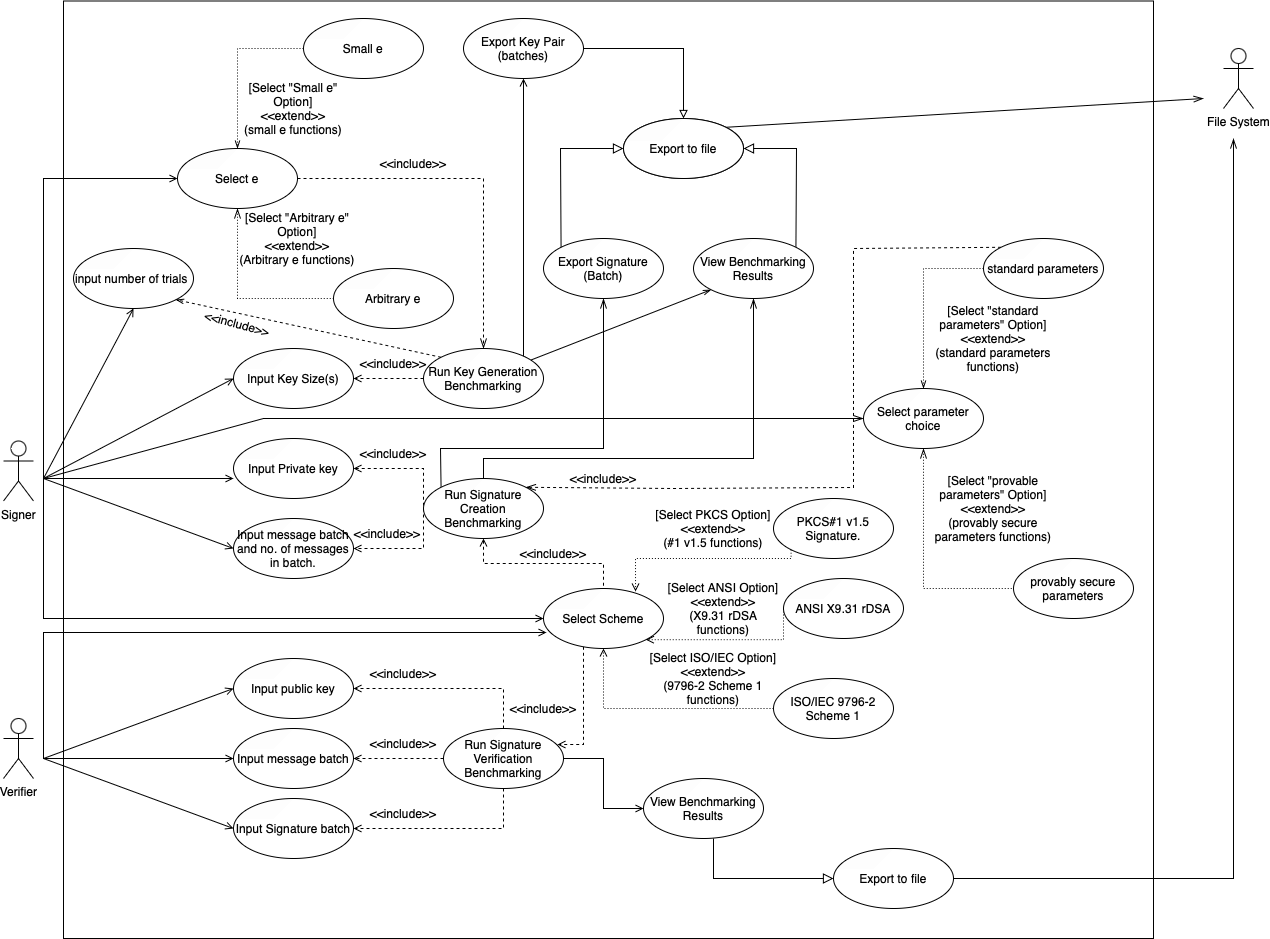
\includegraphics[scale=0.38]{poc_pictures/MAIN_USE-CASE.png}
    \caption{UML Use Case Diagram}
    \label{fig:uc}
\end{figure}



\textbf{Generate Keys Use Case}

\noindent\textbf{Flow of Events:}
\begin{enumerate}
    \item User selects "Generate Key" from the main menu options panel.
    \item User is presented with an input box prompting for the number of keys desired to be generated.
    \item User inputs desired number of keys into the box.
    \item System processes the request and updates the screen with the corresponding of number input boxes displayed vertically down the screen.
    \item System updates the screen with a checkbox labelled small e adjacent to each dynamically generated input box for each key.
    \item User inputs desired key sizes into each of the dynamically generated input boxes, additionally selecting the adjacent "small e" checkbox next to each input box where applicable.
    \item User is presented with an input box labelled enter number of trials for benchmarking run.
    \item User inputs desired number of trials into the box.
    \item System processes the request and completes the benchmarking run for the key generation process.
      \item System displays benchmarking results and notification informing the user that benchmarking process is complete.
      \item User is presented with options ”Export to file” for private key and public key batches corresponding to key pairs generated for all of their entered key configurations in one file.
        \item User is presented with options ”Export to file” for benchmarking results.
        \item User selects desired options for exporting.
\end{enumerate}

\noindent\textbf{Alternative flows:}
\begin{enumerate}
    \item[3a.] User inputs an invalid number of keys.
    \begin{enumerate}
        \item[3a1.] System warns user about the invalid input and prompts them to enter a valid number of keys.
    \end{enumerate}
        \item[4a.] System encounters an error during process of displaying the dynamically generated input boxes.
    \begin{enumerate}
        \item[4a1.] System displays an error message and prompts the user to try again.
    \end{enumerate}
    \item[6a.] User inputs an invalid key size into one of the dynamically generated input boxes.
    \begin{enumerate}
        \item[6a1.] System warns user about the invalid input and prompts them to enter a valid key size .
    \end{enumerate}
     \item[8a.] User inputs an invalid number of trials.
    \begin{enumerate}
        \item[8a1.] System warns user about the invalid input and prompts them to enter a valid number of trials.
    \end{enumerate}
        \item[9a.] System encounters an error during benchmarking of the key generation creation process.
    \begin{enumerate}
        \item[9a1.] System displays an error message and resets screen back to initial view.
    \end{enumerate}  
        \item[10a.]  User selected a small public exponent e for the entire key batch in step 6
    \begin{enumerate}
        \item[10a1.] System preloads provably secure key batches into signature creation and signature verification processes respectively.
    \end{enumerate}
\end{enumerate}



\textbf{Create Signature Use Case}

\noindent\textbf{Flow of Events:}
\begin{enumerate}
    \item User selects "Sign message" from the main menu options panel.
    \item User is presented with text boxes labeled "Input Private Key batch", "Input Message batch" and "Input no. of message".
    \item User provides all required inputs.
    \item User selects the desired signature scheme(s) to be used for benchmarking run from options ("PKCS\#1 v1.5 Signature", "ANSI X9.31 rDSA", ISO\slash IEC 9796-2 scheme 1).
      \item User is presented with radio button selection for Hash Function Size with the options labelled "Custom", "Provably Secure" and "Standard and underneath a drop down menu for selecting a concrete hash function"
        \item User selects "Standard" radio button as option for hash function size
         \item User is presented with solely fixed length hash functions in hash function drop down menu
          \item User selects hash function
          \item User initiates the signature creation benchmarking run by clicking relevant button.
  \item System processes the request and completes the benchmarking run for the signature creation process.
      \item System displays benchmarking results and notification informing the user that benchmarking process is complete.
      \item User is presented with options ”Export to file” for the resulting batch of computed signatures.
       \item User is presented with options ”Export to file” for benchmarking results.
       \item User selects desired options for exporting.
\end{enumerate}

\noindent\textbf{Alternative flows:}
\begin{enumerate}
     \item[2a.] Provably Secure public key batch was preloaded from key generation.
    \begin{enumerate}
     \item[2a1.] The system displays a visual indication that a provably secure private key batch has been preloaded.
    \item[2a2.] User is presented with text boxes labeled "Input Message batch" and "Input no. of message".
    \end{enumerate}
    \item[3a.] User inputs an invalid or mismatched private key batch.
    \begin{enumerate}
        \item[3a1.] System warns user about the invalid input and prompts them to enter a valid private key batch.
    \end{enumerate}
     \item[3b.] User inputs an invalid or mismatched message batch.
    \begin{enumerate}
        \item[3b1.] System warns user about the invalid input and prompts them to enter a valid message batch.
    \end{enumerate}
     \item[3c.] User inputs an invalid number of messages.
    \begin{enumerate}
        \item[3c1.] System warns user about the invalid input and prompts them to enter a valid number of messages.
    \end{enumerate}
         \item[5a.] Provably Secure public key batch was preloaded from key generation.
    \begin{enumerate}
     \item[5a1.] User is presented with radio button selection for instantiating scheme with provably secure parameters with the options labelled "yes", and "no" with currently selected option set to "yes".
    \item[5a2.]  User continues with currently selected yes option
        \begin{enumerate}
      \item[5a2a.] User selects "no" radio button as option for instantiating scheme with provably secure parameters.
    \begin{enumerate}
        \item[5a2a1.] Continue from step 5.
            \end{enumerate}
    \end{enumerate}
    \item[5a3.]  User is presented with radio button selection for Hash Function Size with a single option labelled "Provably Secure" this is currently selected and a drop down menu for selecting a concrete hash function"
     \item[5a4.]  Continue from step 6a1.
    \end{enumerate}
       \item[6a.] User selects "Provably Secure" radio button as option for hash function size
    \begin{enumerate}
        \item[6a1.] User is presented with solely variable length hash functions in hash function drop down menu
         \item[6a2.] The system sets the hash function output size to half the modulus length for each key.
    \end{enumerate}
         \item[6b.] User selects "Custom" radio button as option for hash function size
    \begin{enumerate}
        \item[6b1.] User is presented with solely variable length hash functions in hash function drop down menu
        \item[6b2.] The system prompts the user to input a custom hash size as a fraction e.g., 1/2.
         \item[6b3.] User enters custom hash size.
             \begin{enumerate}
             \item[6b3a.] User inputs invalid custom hash size.
    \begin{enumerate}
        \item[6b3a1.] System displays an error message and prompts the user to try again.
    \end{enumerate}
        \end{enumerate}
         \item[6b4.] The system sets the hash function output size to users specified fraction of modulus length for each key.
    \end{enumerate}
   

    \item[10a.] System encounters an error during benchmarking of the signature creation process.
    \begin{enumerate}
        \item[10a1.] System displays an error message and prompts the user to try again.
    \end{enumerate}
    \item[12a.]  User selected ISO\slash IEC 9796-2 scheme 1 in step 4.
    \begin{enumerate}
        \item[12a1.] User is presented with options "Export to file" for the computed batch of signatures and additionally if applicable a computed batch of non recoverable messages portions.
    \end{enumerate}
\end{enumerate}

\textbf{Verify Signature Use Case}

\noindent\textbf{Flow of Events:}
\begin{enumerate}
    \item User selects "Verify Signature" from the main menu options panel.
    \item User is presented with text boxes labeled "Input public Key batch", "Input Message batch" and "input signature batch".
    \item User provides all required inputs.
       \item User selects the desired signature scheme(s) to be used for benchmarking run from options ("PKCS\#1 v1.5 Signature", "ANSI X9.31 rDSA", ISO\slash IEC 9796-2 scheme 1).
      \item User is presented with radio button selection for Hash Function Size with the options labelled "Custom", "Provably Secure" and "Standard and underneath a drop down menu for selecting a concrete hash function"
              \item User selects "Standard" radio button as option for hash function size
         \item User is presented with solely fixed length hash functions in hash function drop down menu
          \item User selects hash function
               \item User initiates the signature verification benchmarking run by clicking relevant button.
         \item System processes the request and completes the benchmarking run for the signature verification process.
      \item System displays benchmarking results and notification informing the user that benchmarking process is complete.
      \item User is presented with options ”Export to file” for the results of signature verification for each and every message.
       \item User is presented with options ”Export to file” for benchmarking results.
       \item User selects desired options for exporting.
\end{enumerate}


\noindent\textbf{Alternative flows:}
\begin{enumerate}
     \item[2a.] Provably Secure public key batch was preloaded from key generation.
    \begin{enumerate}
     \item[2a1.] The system displays a visual indication that a provably secure private key batch has been preloaded.
    \item[2a2.] User is presented with text boxes labeled "Input Message batch" and "Input no. of message".
    \end{enumerate}
    \item[3a.] User inputs an invalid or mismatched private key batch.
    \begin{enumerate}
        \item[3a1.] System warns user about the invalid input and prompts them to enter a valid private key batch.
    \end{enumerate}
     \item[3b.] User inputs an invalid or mismatched message batch.
    \begin{enumerate}
        \item[3b1.] System warns user about the invalid input and prompts them to enter a valid message batch.
    \end{enumerate}
     \item[3c.] User inputs an invalid number of messages.
    \begin{enumerate}
        \item[3c1.] System warns user about the invalid input and prompts them to enter a valid number of messages.
    \end{enumerate}
         \item[5a.] Provably Secure public key batch was preloaded from key generation.
    \begin{enumerate}
     \item[5a1.] User is presented with radio button selection for instantiating scheme with provably secure parameters with the options labelled "yes", and "no" with currently selected option set to "yes".
    \item[5a2.]  User continues with currently selected yes option
        \begin{enumerate}
      \item[5a2a.] User selects "no" radio button as option for instantiating scheme with provably secure parameters.
    \begin{enumerate}
        \item[5a2a1.] Continue from step 5.
            \end{enumerate}
    \end{enumerate}
    \item[5a3.]  User is presented with radio button selection for Hash Function Size with a single option labelled "Provably Secure" this is currently selected and a drop down menu for selecting a concrete hash function"
     \item[5a4.]  Continue from step 6a1.
    \end{enumerate}
       \item[6a.] User selects "Provably Secure" radio button as option for hash function size
    \begin{enumerate}
        \item[6a1.] User is presented with solely variable length hash functions in hash function drop down menu
         \item[6a2.] The system sets the hash function output size to half the modulus length for each key.
    \end{enumerate}
         \item[6b.] User selects "Custom" radio button as option for hash function size
    \begin{enumerate}
        \item[6b1.] User is presented with solely variable length hash functions in hash function drop down menu
        \item[6b2.] The system prompts the user to input a custom hash size as a fraction e.g., 1/2.
         \item[6b3.] User enters custom hash size.
             \begin{enumerate}
             \item[6b3a.] User inputs invalid custom hash size.
    \begin{enumerate}
        \item[6b3a1.] System displays an error message and prompts the user to try again.
    \end{enumerate}
        \end{enumerate}
         \item[6b4.] The system sets the hash function output size to users specified fraction of modulus length for each key.
    \end{enumerate}
   
    \item[10a.] System encounters an error during benchmarking of the signature creation process.
    \begin{enumerate}
        \item[10a1.] System displays an error message and prompts the user to try again.
    \end{enumerate}
    \item[12a.]  User selected ISO\slash IEC 9796-2 scheme 1 in step 4.
    \begin{enumerate}
        \item[12a1.] The results of signature verification for each and every message in file offered for export, contains text corresponding to recovered portion of message if corresponding signature on message verified correctly.
    \end{enumerate}
\end{enumerate}





\subsection{Acceptance Tests}


\textbf{1. Benchmarking Key Pair Generation:}
\begin{enumerate}
\item Launch the benchmarking application and select "Generate Key" from the main menu.
\item Ensure the application presents an input box for entering the desired number of key pairs for generation.
\item Verify that after inputting the desired number of key pairs, the application dynamically displays corresponding input boxes for each key pair, along with a checkbox labeled 'small e' adjacent to each input box.
\item Check the functionality for the user to input desired key sizes into each dynamically generated input box and the option to select the 'small e' checkbox where applicable.
\item Confirm that the application presents an input box for entering the number of trials for the benchmarking run.
\item Test the process of inputting the desired number of trials and verify that the system processes the request correctly.
\item Inspect the system's ability to complete the benchmarking run for the key generation process without errors or exceptions.
\item Ensure the application displays benchmarking results along with a notification confirming the completion of the benchmarking process.
\item Verify the availability and functionality of the options to export both the most recently benchmarked private and public key batches, as well as the benchmarking results to a file.
\end{enumerate}


\textbf{2. Benchmarking Signature Generation:}
\begin{enumerate}
    \item Navigate to the signature generation section in the application.
    \item Use the option to import a valid message batch.
    \item Use the option to import a valid private key batch.
    \item Check that the application notifies the user if an empty message batch or an invalid private key batch is provided, with instructions to provide valid inputs.
    \item Confirm that the application allows the user to select "Standard", "Provably Secure" or "custom" hash function size.
    \item When "Standard" is selected, verify that only fixed-length hash functions are available for selection.
    \item When "Provably Secure" is selected, verify that variable-length hash functions are available and that the hash function output size is automatically set to half the modulus length for each key.
    \item Ensure the benchmarking of the signature creation process completes without errors.
    \item Confirm the application provides notification upon successful completion of the benchmarking process.
    \item Verify that options to export the generated signatures and benchmarking results are available and functional.
\end{enumerate}

\textbf{2. Benchmarking Signature Generation (Alternative Scenarios):}

\begin{itemize}
    \item If a provably secure private key batch was preloaded prior to navigating to signature generation:
    \begin{enumerate}
        \item Verify that the application indicates that the key batch has been preloaded.
        \item Confirm that the hash function selection is limited to "Provably Secure" options.
    \end{enumerate}
    \item When the "Custom" hash function size is selected:
    \begin{enumerate}
        \item Ensure that the user is prompted to input a custom hash size as a fraction.
        \item Check that an error is displayed if the user inputs an invalid custom hash size, with an option to retry.
    \end{enumerate}
\end{itemize}


\textbf{3. Benchmarking Signature Verification:}
\begin{enumerate}
    \item Navigate to the signature Verification section in the application.
    \item Use the option to import a valid message batch.
    \item Use the option to import a valid public key batch.
    \item Check that the application notifies the user if an empty message batch or an invalid public key batch is provided, with instructions to provide valid inputs.
    \item Confirm that the application allows the user to select "Standard", "Provably Secure" or "custom" hash function size.
    \item When "Standard" is selected, verify that only fixed-length hash functions are available for selection.
    \item When "Provably Secure" is selected, verify that variable-length hash functions are available and that the hash function output size is automatically set to half the modulus length for each key.
    \item Ensure the benchmarking of the signature creation process completes without errors.
    \item Confirm the application provides notification upon successful completion of the benchmarking process.
\item Verify options to export both the generated signature verification results and benchmarking results to a file.
\end{enumerate}

\textbf{3. Benchmarking Signature Verification (Alternative Scenarios):}

\begin{itemize}
    \item If a provably secure public key batch was preloaded prior to navigating to signature verification:
    \begin{enumerate}
        \item Verify that the application indicates that the key batch has been preloaded.
        \item Confirm that the hash function selection is limited to "Provably Secure" options.
    \end{enumerate}
    \item When the "Custom" hash function size is selected:
    \begin{enumerate}
        \item Ensure that the user is prompted to input a custom hash size as a fraction.
        \item Check that an error is displayed if the user inputs an invalid custom hash size, with an option to retry.
    \end{enumerate}
\end{itemize}





\textbf{4. Benchmarking Signature Creation and Verification with PKCS\#1 v1.5:}
\begin{enumerate}
\item Select the PKCS\#1 v1.5 Signature Scheme for benchmarking within the application.
\item Conduct benchmarking of both the signature generation and verification processes with corresponding test batches using the previous steps. Ensure both processes succeed.
\item Verify the functionality to export the benchmarking results for both signature generation and verification processes to a file.
\item Verify the functionality to export the results for the actual verification of signatures to a file.
\end{enumerate}


\textbf{5. Benchmarking Signature Creation and Verification with ANSI X9.31 rDSA:}
\begin{enumerate}
\item Select the ANSI X9.31 rDSA Signature Scheme for benchmarking within the application.
\item Conduct benchmarking of both the signature generation and verification processes with corresponding test batches using the previous steps. Ensure both processes succeed.
\item Verify the functionality to export the benchmarking results for both signature generation and verification processes to a file.
\item Verify the functionality to export the results for the actual verification of signatures to a file.
\end{enumerate}


\textbf{6. Benchmarking Signature Generation with ISO/IEC 9796-2:2010 Scheme 1:}
\begin{enumerate}
\item Set the application to use the ISO/IEC 9796-2:2010 Signature Scheme 1.
\item Conduct benchmarking of  the signature generation process with corresponding test batches using the previous steps and ensure it succeeds.
\item Verify options to export a batch of messages to a file (e.g., as a message recovery mode, non recoverable portion of messages is transmitted along with signature).
\end{enumerate}

\textbf{7. Benchmarking Signature Verification with ISO/IEC 9796-2:2010 Scheme 1:}
\begin{enumerate}
\item Select the ISO/IEC 9796-2:2010 Scheme 1 for benchmarking within the application.
\item Conduct benchmarking of both the signature generation and verification process with corresponding test batches using the previous steps. Ensure both processes succeed.
\item Verify the functionality to export the benchmarking results for the signature verification process to a file.
\item Verify the functionality to export the results for the actual verification of signatures to a file.
\item Check that results for the actual verification of signatures additionally contain recovered message portions.
\end{enumerate}


\section{Appendix B.2 Design}

\textbf{Design of Signature Model Assembly}
\begin{figure}[H]
    \centering
    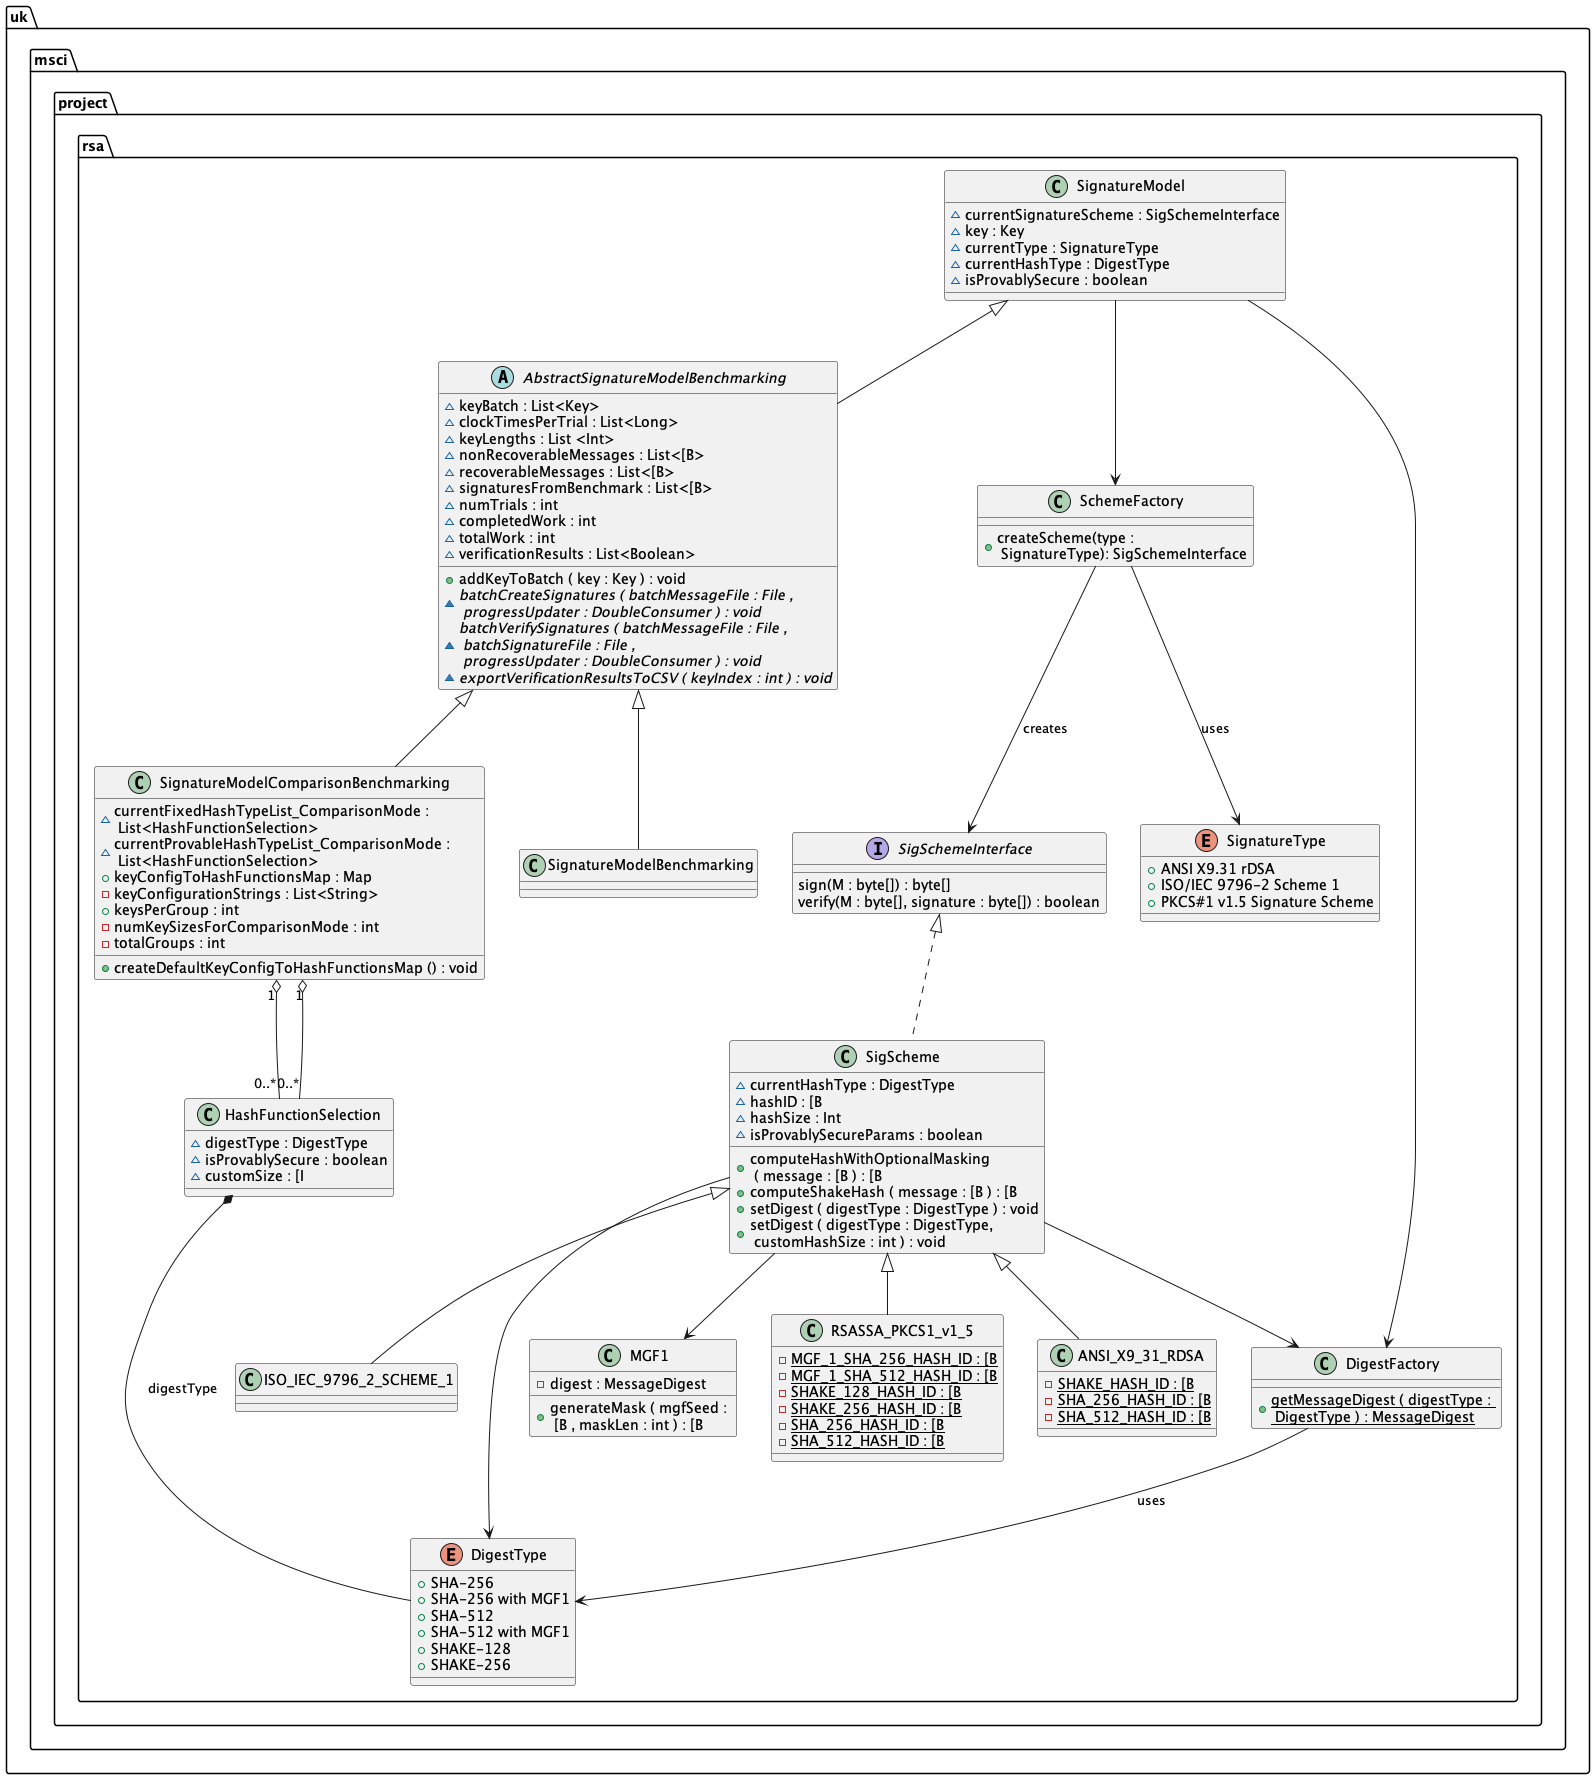
\includegraphics[scale=0.335]{main_pictures/signatureModel.png}
    \caption{Design of Signature Model Assembly}
    \label{fig:SIGMODDESIGN}
\end{figure}

Central to this assembly is the SignatureModel class. It holds the state of a user-initiated digital signature scheme, including the current signature scheme, the associated key, and the digest type. 

Building upon the SignatureModel, the AbstractSignatureModelBenchmarking class extends its capabilities by integrating benchmarking functions. It maintains lists to store trial times, benchmarked signatures, and captures recoverable and non-recoverable parts of messages where applicable

The SignatureModelBenchmarking subclass specialises in conducting batch operations in benchmarking scenarios. This class is designed for efficiency in large-scale data handling by utilising concurrency, managing multiple keys, and processing large volumes of signatures simultaneously.

The SignatureModelComparisonBenchmarking class offers a specialised form of benchmarking to be described as cross-parameter comparison mode. It is designed to extend benchmarking functionality to accommodate comparison benchmarking allowing for the side-by-side evaluation of parameter types for a provided signature scheme. This class is structured to manage and benchmark various key sizes and hash function. It maintains further lists for application on a per key size basis to store keyConfigurationStrings that each uniquely represent a key parameter configuration and a keyConfigToHashFunctionsMap, a mapping that associates each group of key configurations with their respective hash functions. 

\textbf{Factory pattern}

The factory pattern manifests within this assembly through the SchemeFactory class, which simplifies the instantiation of various RSA signature schemes like ANSI X9.31 and ISO/IEC 9796-2. By following the SigSchemeInterface, every signature scheme adheres to a uniform set of operations, ensuring consistency across different implementations.

The DigestFactory pattern, mirrors the factory design of the signature schemes, serves a similar function for hash functions. It encapsulates the complexity of algorithm instantiation, guided by the DigestType. This separation of concerns promotes a clean architecture, allowing for straightforward extensions and modifications.

During the instantiation of a signature scheme with provably secure parameters, the DigestFactory pattern plays a facilitatory role. When a scheme is instantiated with the flag for provably secure parameters set the DigestFactory aids in configuring the MessageDigest to the specified DigestType, adjusting the hash size accordingly (hash function output size of half the modulus length to achieve provable security).

\newpage
\subsection{Key Generation Module}

\textbf{Design of Key Generation Controller Assembly: Orchestration of key generation}

\begin{figure}[H]
    \centering
    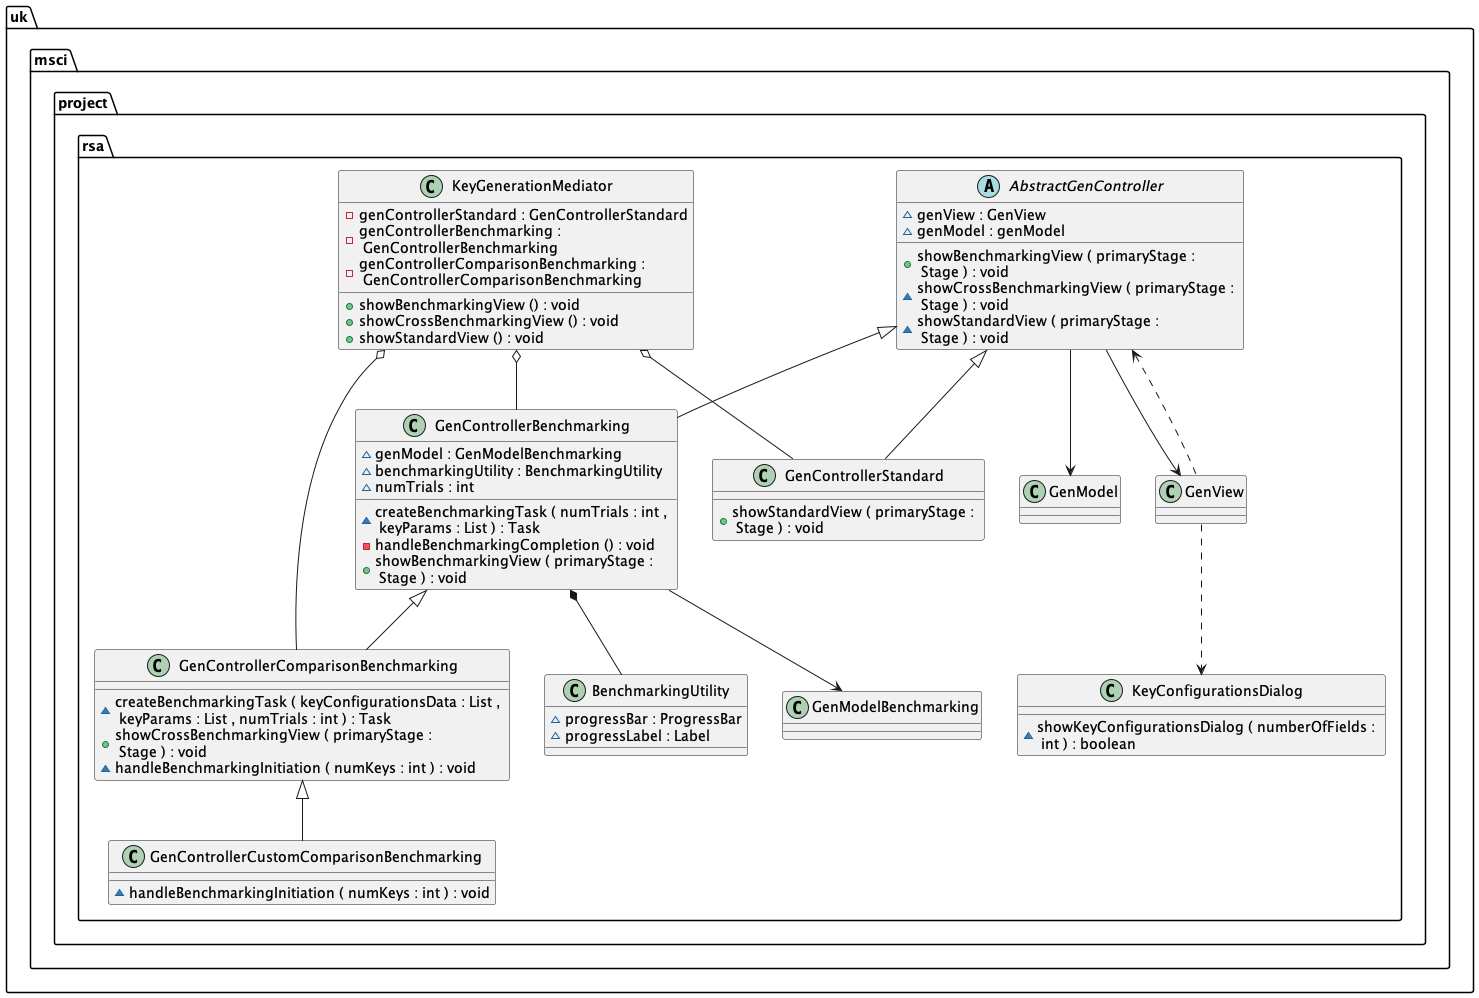
\includegraphics[scale=0.367]{main_pictures/genController.png}
    \caption{Design of Key Generation Controller Assembly: Orchestration of key generation}
    \label{fig:KEYCONTROLLERDESIGN}
\end{figure}

\textbf{KeyGenerationMediator:}

Central to the Key Generation module is the KeyGenerationMediator, serving as the intermediary between the primary MainController and the distinct key generation controllers. The mediator pattern comes into play, facilitating the management of various key generation operational modes—standard, benchmarking, and comparison benchmarking—without overcomplicating the main controller's logic. This mediator ensures that appropriate controllers are activated and configured to match the operational context, whether the user is generating a single key pair or a batch for benchmarking purposes.

\textbf{Controllers:}

The GenControllerBenchmarking class is tailored for benchmarking key generation performance, holding a reference to the GenModelBenchmarking and a BenchmarkingUtility with a ProgressBar for real-time progress indication. It can create tasks for generating keys under given parameters and handle the completion of these tasks, updating the view to reflect results.

The GenControllerStandard is focused on standard, non-benchmarked key generation processes. It provides a straightforward interface to generate keys and output them to the user, signifying a successful operation without the need for analysis.

The GenControllerComparisonBenchmarking in a similar intuition to its signature module equivalent extends benchmarking functionality to accommodate the side-by-side evaluation of key configuration types. This class can initiate benchmarking tasks that compare different parameter type groupings, providing insights into performance differentials between various key configurations at scale for arbitrary key sizes.

In support of the controllers, the GenModel and its subclass GenModelBenchmarking serve as the data models for key generation. They encapsulate the state and logic for key generation operations, providing a structured approach to manage and store generated keys and related data.


\textbf{Design of the Key Generation Model Assembly}


\begin{figure}[H]
    \centering
    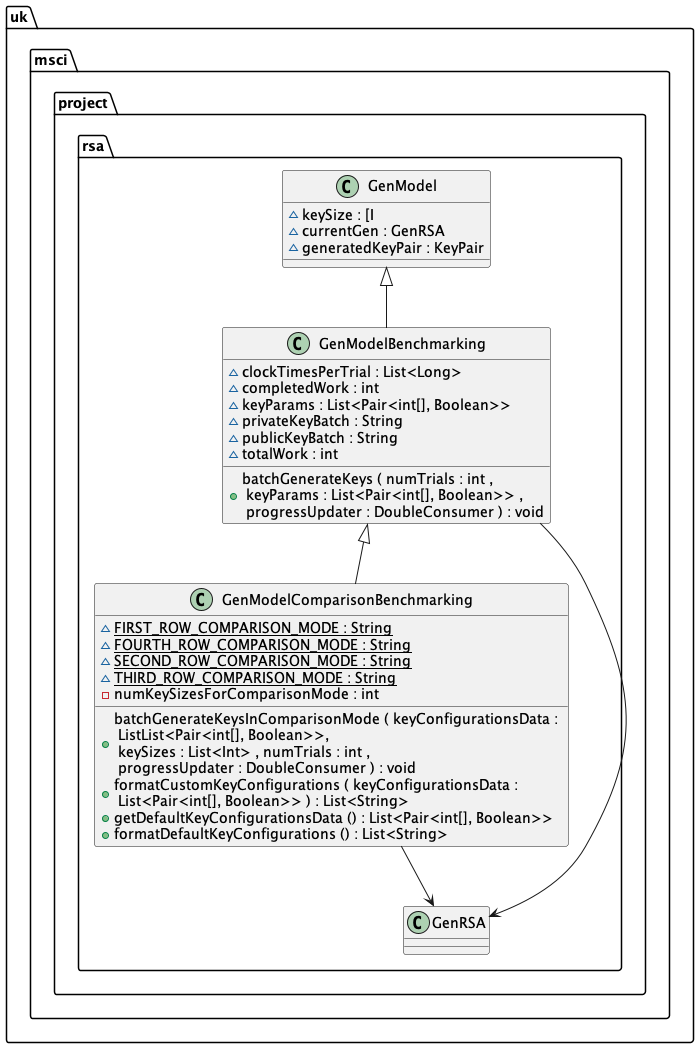
\includegraphics[scale=0.39]{main_pictures/genModel.png}
    \caption{Design of the Key Generation Model Assembly}
    \label{fig:KEYMODEDESIGN}
\end{figure}

The GenModel class encapsulates the attributes and behaviours necessary for RSA key generation, including the key size, the current key generation instance (currentGen), and the resultant KeyPair (generatedKeyPair). This class represents the state of a user-initiated RSA key generation process and provides a foundation for more specialised key generation models.

The GenModelBenchmarking class extends the GenModel to support the benchmarking of RSA key generation. It contains lists for tracking execution times (clockTimesPerTrial) and maintains state related to the key generation process, such as completed and total work indicators. It also holds the key configuration parameters (keyParams) for benchmarking by key size, and the batches of private and public keys generated during benchmarking (privateKeyBatch, publicKeyBatch). This class is responsible for initiating batch RSA key generation tasks, to utilised for performance assessment across various key configurations for specified key sizes.

The GenModelComparisonBenchmarking class further specialises the benchmarking process. It introduces additional attributes for managing comparison modes, such as strings representing the default configuration modes and an integer for the number of key sizes under comparison (numKeySizesForComparisonMode). This class is equipped to perform key generation with user-specified parameters, facilitating direct comparisons between different sets of key configurations. This allows for the evaluation of standard vs. provably secure parameters and user-defined custom parameter sets.



\begin{landscape}
\subsection{Results Module}
\pagestyle{empty}%
\begin{figure}[h]
    \centering
    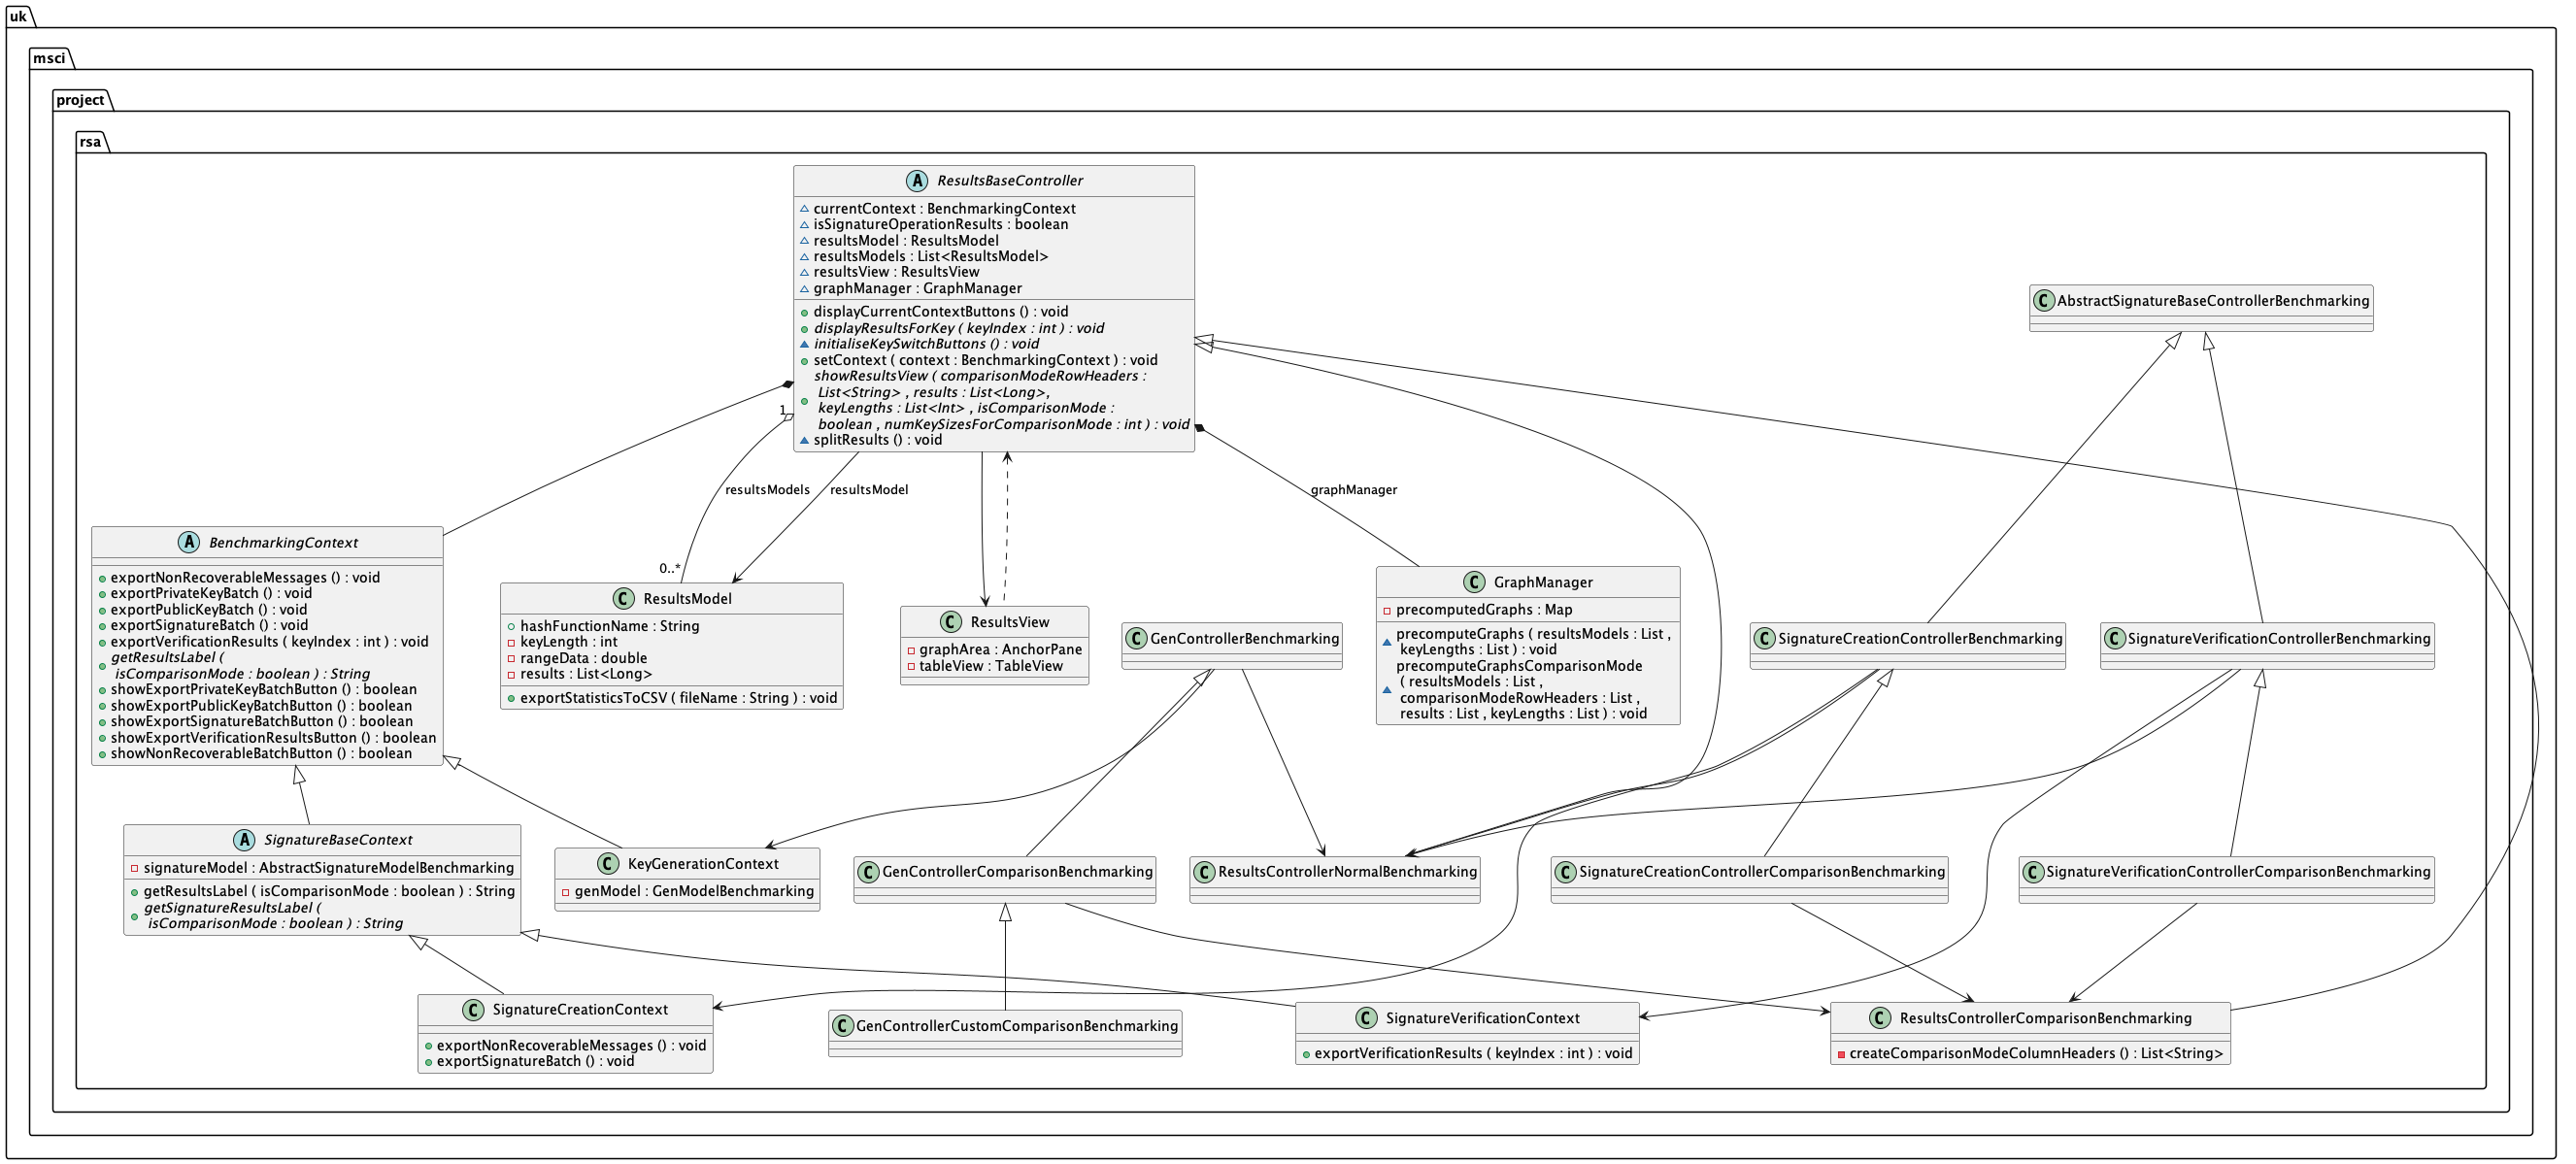
\includegraphics[scale = 0.263]{main_pictures/results.png}
    \caption{Design of the Results Module}
    \label{fig:RESULTSMODULEDESIGN}
\end{figure}
\end{landscape}

The Results Module is designed to process and present the outcome of benchmarking activities. Its core components, the ResultsModel and Results controller assembly, interact to store and manage statistical data, offering insights into the performance of the considered digital signature schemes and/or key generation processes aggregated by key size (e.g., multiple key configurations per each in comparison mode) or by key (in normal benchmarking). 

The ResultsModel serves as the data repository and records an array of time measurements from benchmarking trials, subsequently computing statistical averages like mean, median and percentile values. It is equipped with methods for export functionalities to output the gathered data to CSV files for further use or examination.

The ResultsBaseController, an abstract class, lays the foundation for controllers that manage results display logic. This class holds references to a list of ResultsModel instances, thus supporting the representation of benchmarking results for individual keys. It orchestrates the interaction between the results view and model components, and it provides methods for the initial setup of the results context, display logic for the current benchmarking context, and splitting results for different key configurations.

Inheriting from ResultsBaseController are two specialised controllers: ResultsControllerNormalBenchmarking and ResultsControllerComparisonBenchmarking, each tailored to a specific mode of benchmarking. The ResultsControllerNormalBenchmarking focuses on results related to individual keys. It simplifies the presentation of benchmarking data by concentrating on one key at a time, providing a streamlined and detailed view of its performance metrics. On the other hand, ResultsControllerComparisonBenchmarking is designed for comparison benchmarking mode, facilitating the juxtaposition of performance metrics across different key configurations in their groups and associated group hash functions by key size if results relate to signature operations.

The Results Module integrates with the overarching BenchmarkingContext to ensure that the results displayed are contextually relevant. The BenchmarkingContext and its subclasses manage the visibility of UI components relevant to each benchmarking scenario.

The Results Controller assembly encapsulates a GraphManager responsible for creating and handling various graphical representations of the benchmarking results. It supports different graph types like histograms, box plots, and line graphs, which can be used to visualise the results in both individual key analysis (normal benchmarking mode) and comparative analysis across different key sizes and configurations.




\begin{landscape}
\subsection{UML Package Diagram (All functionality)}
\pagestyle{empty}

\begin{figure}[H]
    \centering
    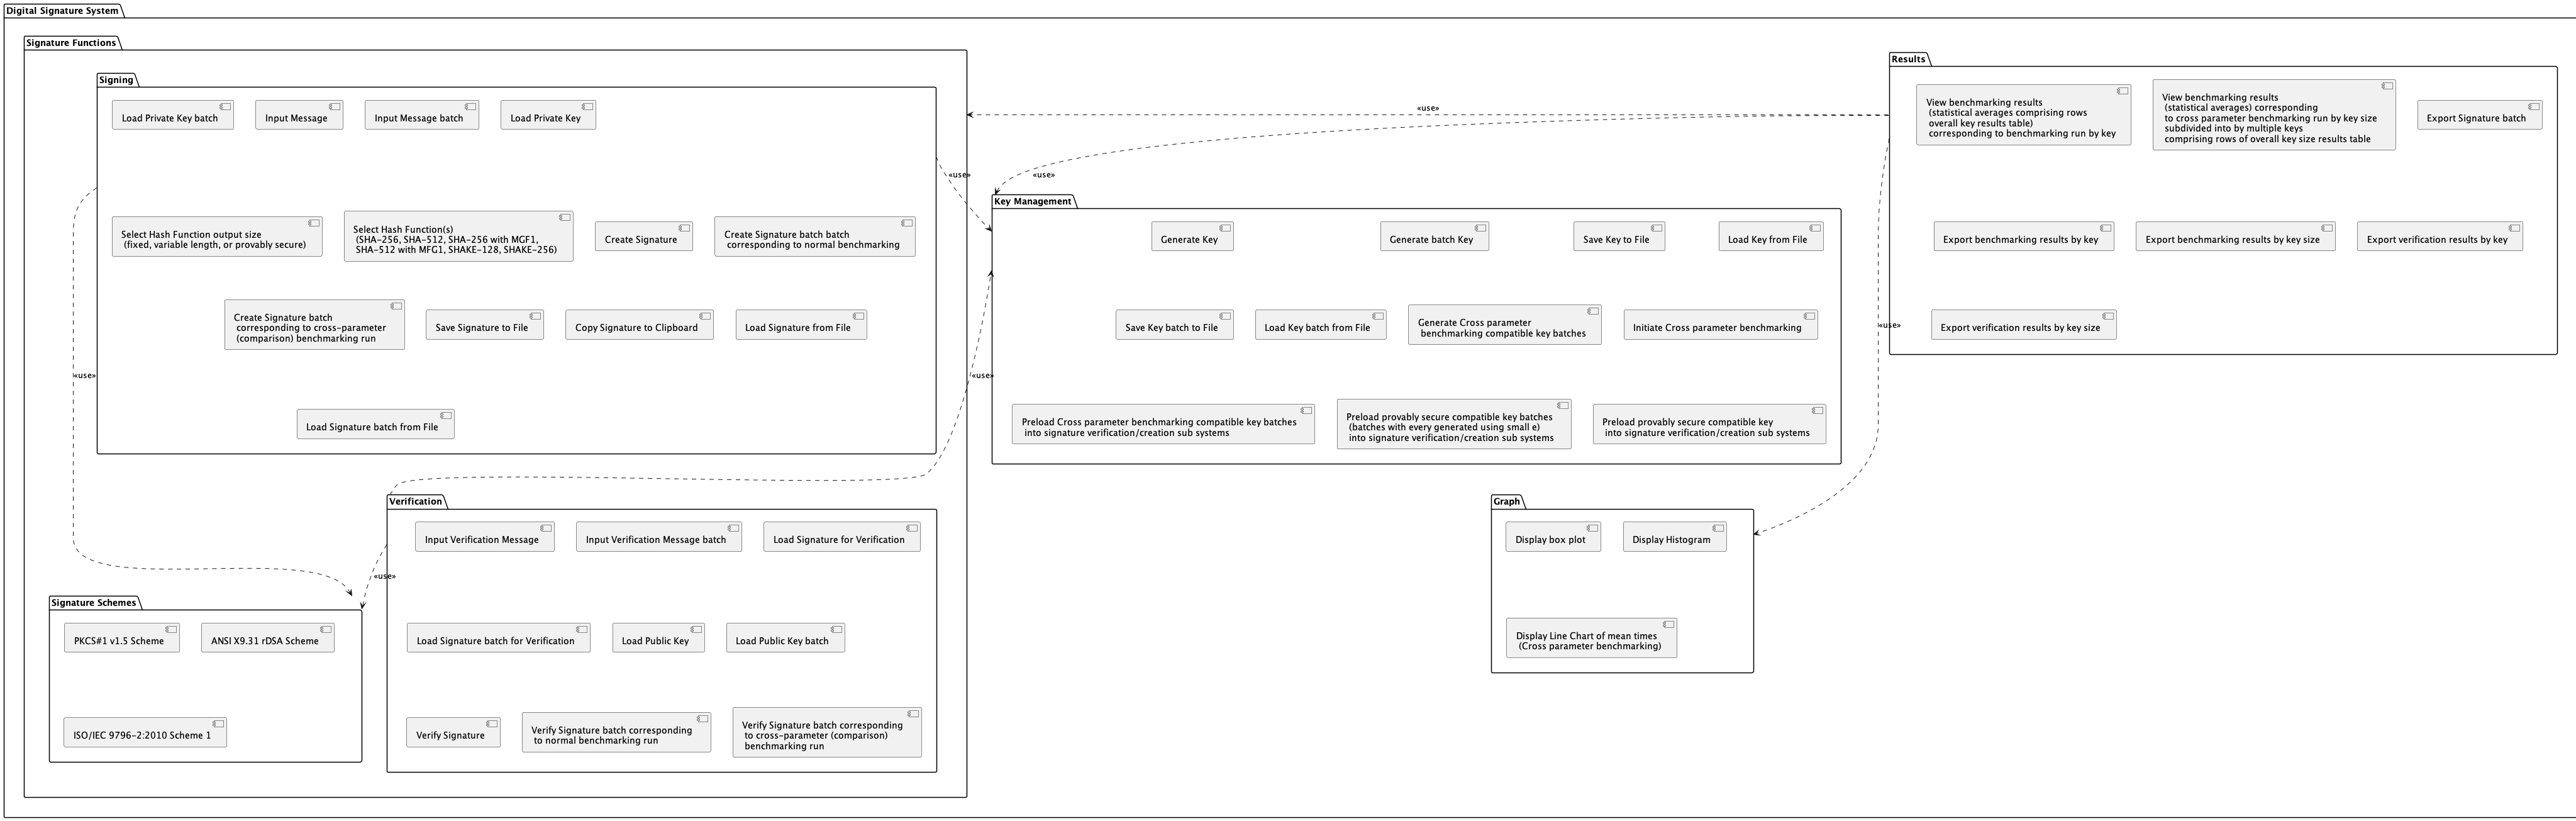
\includegraphics[width=1.1\linewidth]{main_pictures/package.png}
    \caption{UML Package Diagram (All functionality)}
    \label{fig:pack}
\end{figure}
\end{landscape}


Figure \ref{fig:pack} depicts the functionality of the program and is in direct alignment with the full feature set of program as specified across the both the essential and non-essential requirements.

The "Key Management" package is a suite encompassing all key-related operations. It allows for generating individual and batch keys, saving and loading these keys to and from files, and managing keys for cross-parameter benchmarking. It also handles the preloading of keys for signature processes where applicable. For example batches generated using a small public exponent i.e., "provably secure compatible key batches" can be preloaded into signature processes. Additionally in comparison benchmarking mode, it allows users to enter desired key sizes and automatically generates keys for each inputted key size based the 2 groups of key configurations respective to standard and provably secure parameters in sequential order comprising the public-private key batch pairing. This is what can be described as Cross parameter benchmarking compatible key batches and they are preloaded into signature verification/creation sub systems. In Custom comparison mode, keys for each key size can be generated based on arbitrary groups of key configurations (and the hash functions to be used for each group) selected by the user.

Within the "Signature Functions" package, sub-packages are dedicated to signing and verification tasks. They incorporate user inputs, key management, and hash function selection, each tailored to support the considered signature schemes presented in a separate sub-package, including PKCS\#1 v1.5, ANSI X9.31 rDSA, and ISO/IEC 9796-2:2010 Scheme 1. Within standard benchmarking, a singular hash function is selected for uniform application across all key configurations. Cross-parameter benchmarking introduces a divergent selection of hash functions, with fixed-length options (SHA-256 and SHA-512) for standard parameters and variable-length options (SHAKE-128 and SHAKE-256) configured with a hash output of half the length of the modulus  for each key it used with for provably secure parameters. Custom comparison benchmarking forgoes the need for discrete hash function choices during the signature phase by preloading selections during the key generation phase e.g., hash function selections for each group of custom key configurations specified by a user are entered during key generation when the group is defined obviating the need for the user to provide a selection during the signature phase.

The "Results" package deals with the presentation and export of benchmarking outcomes. It ensures the user can view and export benchmarking results by key (normal benchmarking) or by key size (comparison benchmarking),
Lastly, the "Graph" package offers a visual representation of statistical data. It contains functionality to display box plots, histograms, and line charts, particularly useful for cross-parameter benchmarking results, enhancing the user's understanding of the data.


\textbf{Benchmarking Modalities}

\begin{itemize}
    \item \textbf{Normal Benchmarking}: The system provides a straightforward assessment of the relevant process, offering the user key-specific benchmarking results. For signature operations, the same hash function is applied to every key configuration.
     \item \textbf{Comparison Benchmarking (Standard vs. Provably Secure)}: This mode offers a direct comparative analysis between standard and provably secure key configuration groups (with user selected hash functions for each group). The user can then evaluate the performance of the two Standard and Provably Secure groupings, with all trials repeated for each hash function within each group. Results are presented side by side in a table and/or overlaid graphs for each entered key size.
 \item \textbf{Custom Comparison Benchmarking}: In this mode, users have the flexibility to specify key configurations and corresponding hash functions for each group. They can then assess the performance of their chosen key configuration groupings, with all trials repeated for each hash function within each group. Results are presented side by side in a table and/or overlaid graphs for each entered key size.
\end{itemize}

Dependencies between these packages indicate a flow of data and usage across the system. For example, the "Results" package uses data generated by "Signature Functions" and "Key Management," and also utilises the "Graph" package for displaying results, signifying a cohesive and interrelated system design.


\subsection{UML sequence diagrams (Normal Benchmarking functionality only)}
\begin{figure}[H]
    \centering
    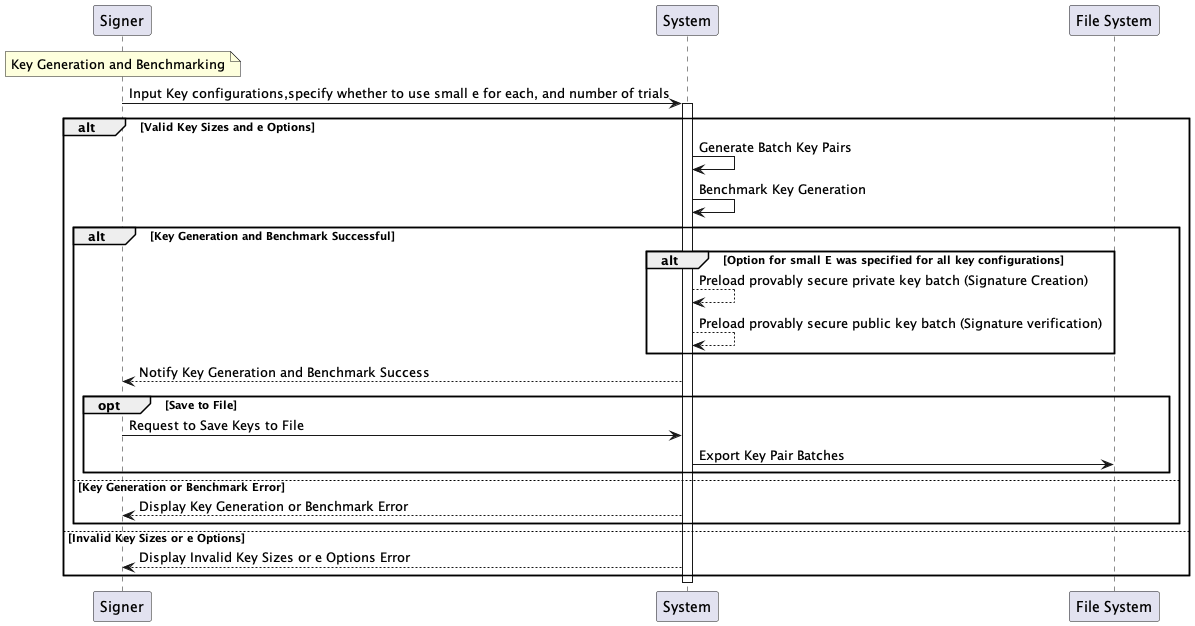
\includegraphics[scale=0.42]{main_pictures/sequenceKey.png}
    \caption{UML Sequence Diagram (Key Generation)}
    \label{fig:uc}
\end{figure}

The above diagram outlines the steps taken by a user within the system to configure and execute the key generation process, which is critical for both the signature creation and verification phases.

The process begins when the user inputs the key configurations, indicating the desired key size and whether to utilise a small public exponent (e) for each key. The system then proceeds to generate a batch of key pairs and benchmarks the key generation process, provided the key sizes and options are valid. An alternate path allows for the preloading of provably secure key batches if the option for a small e was specified for all key configurations,.

Upon successful completion, the user is notified, benchmarking results are displayed and there is an option to save the generated keys to a file. This action interacts with the file system to persist the key batches. Should there be an error during key generation or benchmarking, or if the provided key sizes or options are invalid, the system displays the appropriate error message.

\begin{figure}[H]
    \centering
    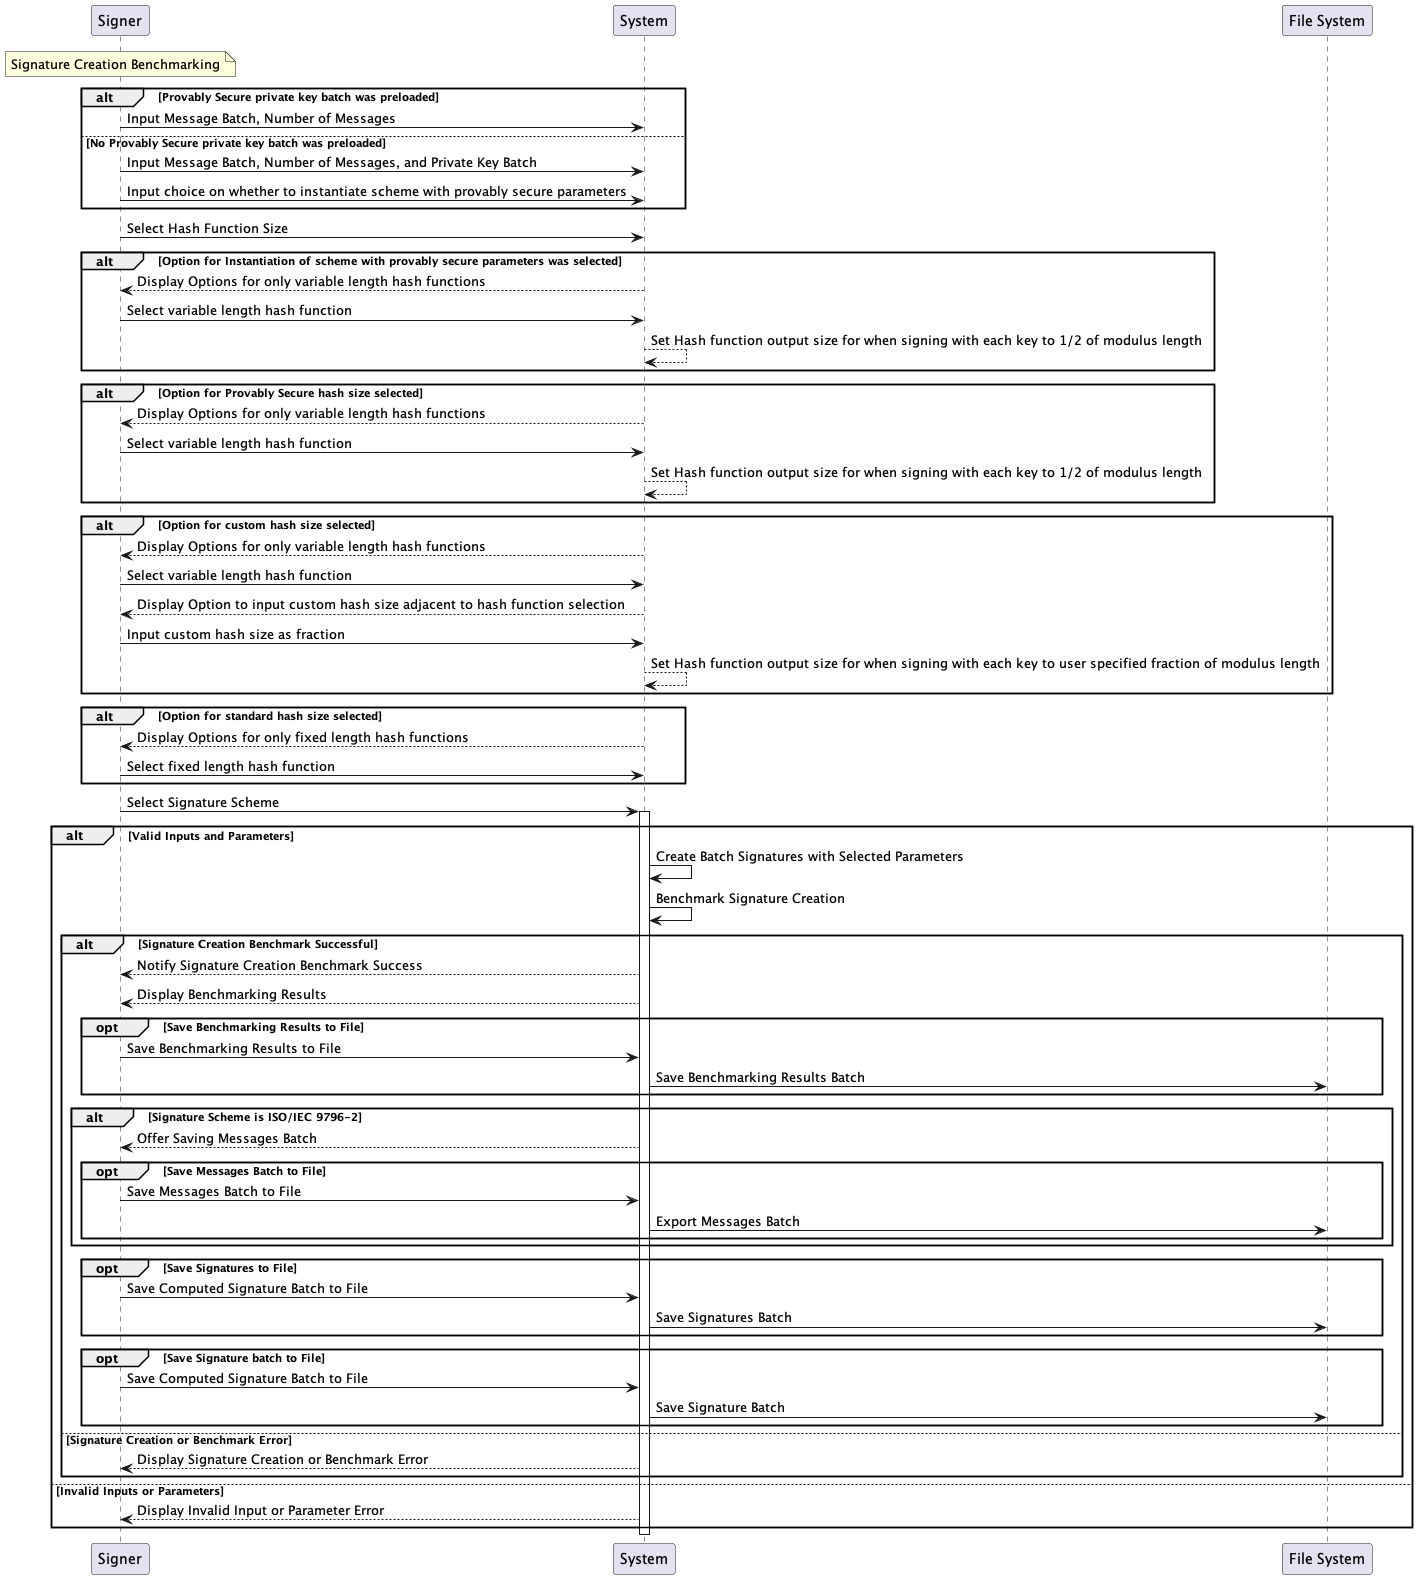
\includegraphics[scale=0.34]{main_pictures/sequenceSign.png}
    \caption{UML Sequence Diagram (Signature Creation)}
    \label{fig:uc}
\end{figure}

The Signature Creation sequence diagram portrays the steps for digital signature generation. The sequence begins with a potential bypass: if a provably secure public key batch was preloaded—contingent upon the selection of a small public exponent e for the entire key batch during the Key Generation phase—the system obviates the need for the user to provide a private key batch.
The system presents the hash function selection as a decision point:
\begin{itemize}
    \item \textbf{Provably Secure Parameters}: If the option for instantiation with provably secure parameters is selected, the system displays only the variable length hash functions. After the user selects one, the system sets the hash function output size to half the modulus length for each key.
    \item \textbf{Provably Secure Hash Size}: If the user opts for a provably secure hash size, the system again displays only variable length hash functions. Upon selection, the output size is configured to half of the modulus length, aligning with provable security standards.
    \item \textbf{Custom Hash Size}: When a custom hash size is chosen, the user is presented with variable length hash functions. The system then prompts the user to input a custom hash size as a fraction, which it uses to determine the hash function output size in relation to the modulus length of each key.
    \item \textbf{Standard Hash Size}: If the standard hash size is preferred, the system limits the display to fixed length hash functions, from which the user can select.
\end{itemize}

Finally, the user selects a message batch and a signature scheme , completing the setup for signature generation. Following these selections, the system generates a batch of signatures and benchmarks their creation. It then provides the user with the results, including options to save the generated signatures and the benchmarking statistics. 

In the Signature Creation sequence, specialised functionality comes into play when implementing message recovery signature schemes such as the ISO/IEC 9796-2 Scheme 1. These schemes require special consideration because their behaviour differs from the standard digital signature process. The ISO/IEC 9796-2 schemes incorporate message recovery features, where part or all of the original message can be reconstructed from the signature itself. This necessitates additional logic in the signing process. The system offers export for a non-recoverable message batch in such cases where each entry is preceded by a "1" if a non-recoverable message follows, whereas a "0" flag denotes the absence of such a message part.


\begin{figure}[H]
    \centering
    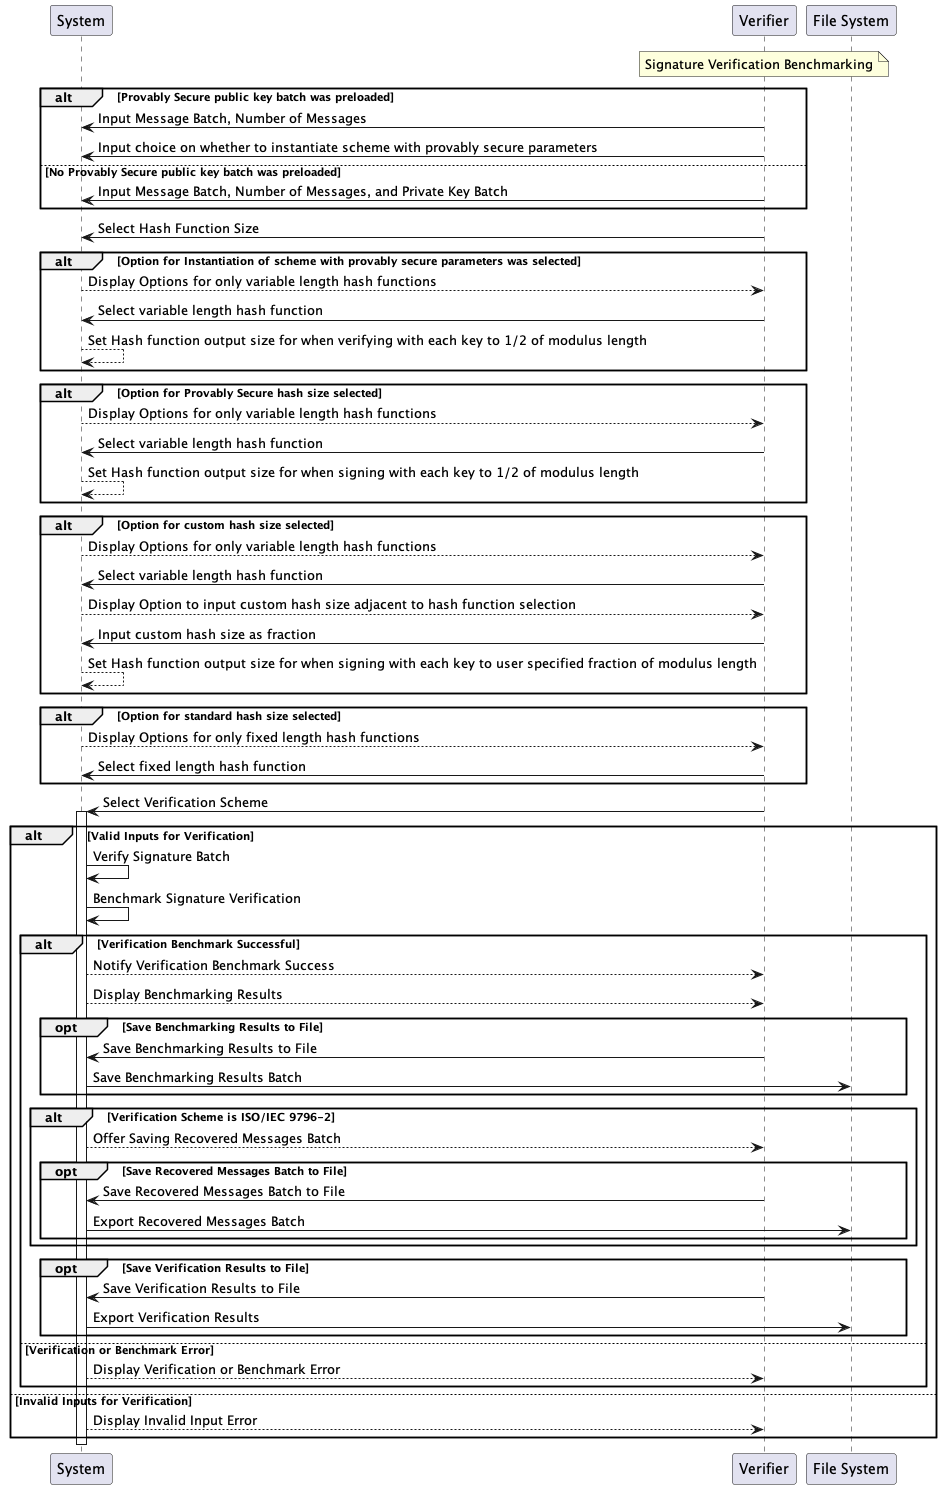
\includegraphics[scale=0.4]{main_pictures/sequenceVerify.png}
    \caption{UML Sequence Diagram (Signature Verification)}
    \label{fig:uc}
\end{figure}

The Signature Verification sequence diagram portrays the steps for digital signature verification. The sequence begins with the same potential bypass relating to the preload of a key batch (but this time around for a public key batch) i.e.,  if a provably secure public key batch was preloaded the system obviates the need for the user to provide a public key batch.
As with signature creation, the user encounters the equivalent decision point regarding hash function size hash function selection:

Following this the user then selects a message batch and a signature scheme, completing the setup for signature generation. Following these selections, the system generates a batch of signatures and benchmarks their creation. It then provides the user with the results, including options to save the generated signatures and the benchmarking statistics. 

For signatures associated with message recovery i.e., ISO/IEC 9796-2 Scheme 1, the sequence accommodates a vital step where the message batch inputted by the verifier should be the non recoverable message batch file exported after the conclusion of the signature creation benchmarking. Such a file contains entries (corresponding to signatures in a one-to-one line by line basis) starting with a "1" or "0" flag to indicate the presence or absence of non-recoverable message parts. The system will then use the non recoverable part when applicable for a signature entry to generate the contents of a recovered message batch which is offered as part of the verification results export.





 

\section{Appendix B.3 Testing}

\subsection{Appendix B.3A Integration Testing}
My approach towards integration testing was tailored to ensure that each of the application modules functioned correctly within their respective Model-View-Controller (MVC) frameworks. Utilising TestFX \cite{TestFX2023}, a testing framework for JavaFX applications, the testing concentrated on the internal workings of each module, examining how well the MVC components within a single module interacted with each other.

The first step of this testing was to ensure that the main controller effectively managed transitions from the application-level main menu into the different functional modules. 

The primary role of TestFX in this scenario was to automate interactions within each module, testing the cohesion between the Model, View, and Controller layers. For example, in the key generation module, TestFX helped ensure that the user input in the View layer was accurately processed by the Controller, and the resulting data was correctly managed and reflected by the Model. This pattern was replicated in the signature module that encapsulates the signature creation and verification functionalities as well.



\subsection{Appendix B.3B System Testing}
In the context of the project, my approach to system testing has been focused across the full range of benchmarking functionality.
This focus included not only the primary benchmarking requirements but also the extended to cross-parameter benchmarking features. The latter, initially considered non-essential, is the direct feature that was used to deliver on the aims of the project.


Given the extensive scope of testing necessitated by the expanded functionalities, my strategy to system testing was to prioritise the most critical paths required for the benchmarking. This involved conducting tests on small-scale batches of data and  key configurations, such as 2/3 prime 1024-bit and 2048-bit key setups. The aim was to ensure the applications accurate performance under a selection of critical, yet limited, normal use scenarios. As part of this, I conducted happy path Testing to confirm that the application behaved as expected in ideal conditions.

Due to the breadth of content, comprehensive testing for errors and edge cases was not entirely possible. However, I did engage in some basic negative testing to ensure that the system could handle common user input errors gracefully. This included tests for typical input mistakes and unexpected user actions to a reasonable extent.

Overall, this approach provided me with a sufficient level of confidence in the application's operational integrity and usability.

\begin{comment}
The results from this phase have been succinctly documented, with an emphasis on the performance of the application's key features. These findings are instrumental in my initial evaluation of the system's feasibility and highlight potential areas for further development in subsequent iterations." 
\end{comment}



\begin{table}[H]

  \centering

  \label{tab:table1}
  \resizebox{\textwidth}{!}{%
    \begin{tabular}{|l|p{1.5cm}|p{1.8cm}|p{2.5cm}|p{3.5cm}|p{2.3cm}|}
      \hline
      \textbf{Type of
Testing} & \textbf{Module Scope} & \textbf{Goal of tests} & \textbf{Test Objective} & \textbf{Technique} & \textbf{Completion Criteria}\\
      \hline
      Functional Testing  & All Modules. & The goals of these tests are to verify acceptance of data, its retrieval, and the correct adoption of requirement related logic & Ensure entry and retrieval of data along expected navigation of an application & Execute function, using valid/invalid data, ensuring:
\begin{itemize} \item When valid /invalid data is inputted, respectively, the expected results occur, or corresponding error message is displayed.
\item Each requirement is met. \end{itemize} & All planned tests have been executed\\
     
      \hline
    \end{tabular}%
  }
\end{table}


\begin{table}[H]
   \caption{\textbf{Main Menu Test Cases}}
  \centering
  \label{tab:table1}
  \resizebox{\textwidth}{!}{
    \begin{tabular}{|l|p{2.5cm}|p{2.5cm}|p{2.5cm}|p{2.5cm}|p{3.5cm}|}
      \hline
      \textbf{Test ID} & \textbf{Prerequisites} & \textbf{Test Steps} & \textbf{Test Data} & \textbf{Expected Result} & \textbf{Actual Result}\\
      \hline
      MainMenu-001 & Application is launched and the user is presented with the main menu. & 
      \begin{enumerate}
      \item Click on the "[K] Generate Keys" button.
      \end{enumerate} & N/A & The application should navigate to the key generation page without errors. & Pass \\
      \hline
      MainMenu-002 & Application is launched and the user is presented with the main menu. & 
      \begin{enumerate}
      \item Click on the "[S] Sign Document" button.
      \end{enumerate} & N/A & The application should navigate to the signature creation page without errors. & Pass \\
      \hline
      MainMenu-003 & Application is launched and the user is presented with the main menu. & 
      \begin{enumerate}
      \item Click on the "[V] Verify Signature" button.
      \end{enumerate} & N/A & The application should navigate to the signature verification page without errors. & Pass \\
      \hline
    \end{tabular}%
  }
\end{table}

\section{Appendix B.3C Key Generation (Benchmarking) Tests}








\begin{comment}
\begin{longtable}{|l|p{2.5cm}|p{2.5cm}|p{2.5cm}|p{2.5cm}|p{3cm}|}
  \caption{\textbf{Key Generation Test Cases}}
  \hline
  \textbf{Test ID} & \textbf{Prerequisites} & \textbf{Test Steps} & \textbf{Test Data} & \textbf{Expected Result} & \textbf{Actual Result} \\
  \hline
  KeyGen-001 & Application is installed and operational; the user is on the Key Generation page. & 
  \begin{enumerate}
  \item Navigate to the "Generate Keys" section.
  \item Enter a valid bit size in the input field.
  \item Click the "Generate Keys" button.
  \end{enumerate} & 1024, 1024 & The system should generate a key pair using the specified bit sizes without errors. & Pass \\
  \hline
  KeyGen-002 & Application is installed and operational; the user is on the Key Generation page. & 
  \begin{enumerate}
  \item Navigate to the "Generate Keys" section.
  \item Enter a string of special characters in the input field.
  \end{enumerate} & @\#\%\&*[(\$ & The system should not accept the input and display an error message indicating that only numerical bit sizes are valid & Pass \\
  \hline
  KeyGen-003 & Application is installed and operational; the user is on the Key Generation page. & 
  \begin{enumerate}
  \item Navigate to the "Generate Keys" section.
  \item Enter an excessively long string of numbers in the input field.
  \item Click the "Generate Keys" button.
  \end{enumerate} & A string of numbers exceeding normal bit size lengths (e.g., 1000 digits). & The system should reject the input and display an error message indicating that the bit size is too long and not valid. & \textcolor{red}{Fail.} \\
  \hline
  KeyGen-004 & Application is installed and operational; the user is on the Key Generation page. & 
  \begin{enumerate}
  \item Navigate to the "Generate Keys" section.
  \item Enter alphanumeric characters in the input field.
  \item Click the "Generate Keys" button.
  \end{enumerate} & abc123 & The system should not accept the input and should display an error message that only numeric values are valid. & Pass \\
  \hline
  KeyGen-201 & Application is installed and operational; the user has successfully generated keys using the "Generate Keys" feature. & 
  \begin{enumerate}
  \item After key generation, click on the "Export Private Key" button.
  \item Check the application's default save location for the presence of the new signature file.
  \end{enumerate} & N/A (The action uses the application's UI) & The signature file is automatically saved to the default location specified by the application. The file should contain the correct signature data, formatted as expected for a digital signature. & Pass \\
  \hline
\end{longtable}
\end{comment}








\begin{longtable}{|l|p{2.5cm}|p{2.5cm}|p{2.5cm}|p{2.5cm}|p{3cm}|}
  \caption{\textbf{Key Generation Benchmarking: Invalid Number of Keys Test Cases}}
  \hline
  \textbf{Test ID} & \textbf{Prerequisites} & \textbf{Test Steps} & \textbf{Test Data} & \textbf{Expected Result} & \textbf{Actual Result} \\
  \hline
  KeyGen-001 & Application is installed and operational; the user is on the Key Generation page. & 
  \begin{enumerate}
  \item Navigate to the "Generate Keys" section.
  \item Enter a valid positive value in the input field for number of keys.
  \item Click the "Submit" button.
  \end{enumerate} & 2 & The system should display the dialog for entering a number key configurations  in 2 text fields displayed vertically. & Pass \\
  \hline
  KeyGen-002 & Application is installed and operational; the user is on the Key Generation page. & 
  \begin{enumerate}
  \item Enter a string of special characters in the input field for number of keys.
    \item Click the "Submit" button.
  \end{enumerate} & @\#\%\&*[(\$ & The system should not accept the input and display an error message indicating that only numerical number of key values are valid & Pass \\
  \hline
   KeyGen-003 & Application is installed and operational; the user is on the Key Generation page. & 
  \begin{enumerate}
  \item Enter alphanumeric characters in the input field for number of keys.
  \item Click the "Submit" button.
  \end{enumerate} & adewfrgtrvb
  c125663 & The system should not accept the input and should display an error message that only numeric values are valid. & Pass \\
  \hline
   KeyGen-004 & Application is installed and operational; the user is on the Key Generation page. & 
  \begin{enumerate}
  \item Leave the input field for number of keys empty.
  \item Click the "Submit" button.
  \end{enumerate} &  & The system should not accept the input and should display an error message that only numeric values are valid. & Pass \\
  \hline
   KeyGen-005 & Application is installed and operational; the user is on the Key Generation page. & 
  \begin{enumerate}
  \item Enter a decimal number in the input field for number of keys.
  \item Click the "Submit" button.
  \end{enumerate} & 7.8  & The system should not accept the input and should display an error message that only positive integer values are valid. & Pass \\
  \hline
     KeyGen-006 & Application is installed and operational; the user is on the Key Generation page. & 
  \begin{enumerate}
  \item Enter a negative number in the input field for number of keys.
  \item Click the "Submit" button.
  \end{enumerate} & -5 & The system should not accept the input and should display an error message that only positive integer values are valid. & \textcolor{red}{Fail.} \\
  \hline
    KeyGen-007 & Application is installed and operational; the user is on the Key Generation page. & 
  \begin{enumerate}
  \item Enter a zero in the input field for number of keys.
   \item Click the "Submit" button.
  \end{enumerate} & 0 & The system should not accept the input and should display an error message that only positive integer values are valid. & \textcolor{red}{Fail.} \\
  \hline
    KeyGen-008 & Application is installed and operational; the user is on the Key Generation page. & 
  \begin{enumerate}
  \item Enter a fraction in the input field for number of keys.
  \item Click the "Submit" button.
  \end{enumerate} & 1/2 & The system should not accept the input and should display an error message that only positive integer values are valid. & Pass \\
  \hline
\end{longtable}




\begin{longtable}{|p{1.5cm}|p{2.5cm}|p{3.5cm}|p{2.5cm}|p{3cm}|p{2cm}|}
  \caption{\textbf{Key Generation Benchmarking: Invalid Key Configuration Test Cases}} \\
  \hline
  \textbf{Test ID} & \textbf{Prerequisites} & \textbf{Test Steps} & \textbf{Test Data} & \textbf{Expected Result} & \textbf{Actual Result} \\
  \hline
  KeyGen-009 & Application is installed and operational; the "Generate Keys" dialog is open with 2 input fields for key configurations. & 
  \begin{enumerate}
  \item Leave all text fields empty.
  \item Click the "OK" button.
  \end{enumerate} & & All text fields should display a red background indicating an error. & Pass \\
  \hline
  KeyGen-010 & Application is installed and operational; the "Generate Keys" dialog is open with 2 input fields for key configurations.; the first text field contains "512,512". & 
  \begin{enumerate}
  \item Leave the second text field empty.
  \item Click the "OK" button.
  \end{enumerate} & & The second text field should display a red background indicating an error. & Pass \\
  \hline
  KeyGen-011 & Application is installed and operational; the "Generate Keys" dialog is open with 2 input fields for key configurations.l; the first text field contains "512,512". & 
  \begin{enumerate}
  \item Enter "1024" in the second text field (less than required prime factors).
  \item Click the "OK" button.
  \end{enumerate} & 1024 & The second text field should display a red background indicating an error. & Pass \\
  \hline
  KeyGen-012 & Application is installed and operational; the "Generate Keys" dialog is open with 2 input fields for key configurations; the first text field contains "512,512". & 
  \begin{enumerate}
  \item Enter special characters in the second text field.
  \item Click the "OK" button.
  \end{enumerate} & !@\#\$\% & The second text field should display a red background indicating an error. & Pass \\
  \hline
  KeyGen-013 & Application is installed and operational; the "Generate Keys" dialog is open with 2 input fields for key configurations; the first text field contains "512,512". & 
  \begin{enumerate}
  \item Enter an excessively long numeric input in the second text field.
  \item Click the "OK" button.
  \end{enumerate} & 111111111111
  1111111111
  1111111111
  111111 & The second text field should display a red background indicating an error. & Pass \\
  \hline
  KeyGen-014 & Application is installed and operational; the "Generate Keys" dialog is open with 2 input fields for key configurations; the first text field contains "512,512". & 
  \begin{enumerate}
  \item Enter an alphanumeric input in the second text field.
  \item Click the "OK" button.
  \end{enumerate} & abc123 & The second text field should display a red background indicating an error. & Pass \\
  \hline
    KeyGen-015 & Application is installed and operational; the "Generate Keys" dialog is open with 2 input fields for key configurations; the first text field contains "512,512". & 
  \begin{enumerate}
  \item Enter an output marginally greater than the upper bound limit on key size of 7168
  \item Click the "OK" button.
  \end{enumerate} & 3584, 3855 & The second text field should display a red background indicating an error. & \textcolor{red}{Fail.} \\
  \hline
    KeyGen-016 & Application is installed and operational; the "Generate Keys" dialog is open with 2 input fields for key configurations; the first text field contains "512,512". & 
  \begin{enumerate}
  \item Enter an output marginally lower than the lower bound minimum on key size of 1024
  \item Click the "OK" button.
  \end{enumerate} & 512, 511 & The second text field should display a red background indicating an error. & \textcolor{red}{Fail.} \\
  \hline
    \hline
    KeyGen-017 & Application is installed and operational; the "Generate Keys" dialog is open with 2 input fields for key configurations; the first text field contains "512,512". & 
  \begin{enumerate}
  \item Enter an output greater than the upper bound limit on key size of 7168
  \item Click the "OK" button.
  \end{enumerate} & 5000, 5000 & The second text field should display a red background indicating an error. & \textcolor{red}{Fail.} \\
  \hline
    KeyGen-018 & Application is installed and operational; the "Generate Keys" dialog is open with 2 input fields for key configurations; the first text field contains "512,512". & 
  \begin{enumerate}
  \item Enter a 3 prime output lower than the lower bound minimum on key size of 1024
  \item Click the "OK" button.
  \end{enumerate} & 256, 110, 110 & The second text field should display a red background indicating an error. & \textcolor{red}{Fail.} \\
  \hline
\end{longtable}

\begin{longtable}{|p{1.5cm}|p{2.5cm}|p{3.5cm}|p{2.5cm}|p{3cm}|p{2cm}|}
  \caption{\textbf{Key Generation Benchmarking: Valid Key Configuration Test Cases}} \\
  \hline
  \textbf{Test ID} & \textbf{Prerequisites} & \textbf{Test Steps} & \textbf{Test Data} & \textbf{Expected Result} & \textbf{Actual Result} \\
  \hline
  KeyGen-019 & Application is installed and operational; the "Generate Keys" dialog is open with input fields for key configuration. & 
  \begin{enumerate}
  \item Input "2" in the number of keys text field.
  \item Input valid key configurations as per test data with boolean in brackets representing selection for a small e value.
  \item Click the "Submit" button.
  \end{enumerate} & KeyConfig1: "512,512" (True) KeyConfig2: "1024,1024" (True) & The "Number of Trials" dialog should be displayed, indicating successful input of key configurations. & Pass \\
  \hline
  KeyGen-020 & As above & As above & KeyConfig1: "512,512" (True) KeyConfig2: "1024,1024" (False) & As above & Pass \\
  \hline
  KeyGen-021 & As above & As above & KeyConfig1: "512,512" (False) KeyConfig2: "1024,1024" (True) & As above & Pass \\
  \hline
  KeyGen-022 & As above & As above & KeyConfig1: "512,512" (False) KeyConfig2: "1024,1024" (False) & As above & Pass \\
  \hline
  KeyGen-023 & As above & As above & KeyConfig1: "1024,1024" (True) KeyConfig2: "1024,1024" (True) & As above & Pass \\
  \hline
  KeyGen-024 & As above & As above & KeyConfig1: "1024,1024" (True) KeyConfig2: "1024,1024" (False) & As above & Pass \\
  \hline
  KeyGen-025 & As above & As above & KeyConfig1: "1024,1024" (False) KeyConfig2: "1024,1024" (True) & As above & Pass \\
  \hline
  KeyGen-026 & As above & As above & KeyConfig1: "1024,1024" (False) KeyConfig2: "1024,1024" (False) & As above & Pass \\
  \hline
  KeyGen-027 & As above & As above & KeyConfig1: "256,256,512" (False) KeyConfig2: "384,384,768" (True) & As above & Pass \\
  \hline
  KeyGen-028 & As above & As above & KeyConfig1: "512,512,1024" (True) KeyConfig2: "1280,1280,2560" (False) & As above & Pass \\
  \hline
  KeyGen-029 & As above & As above & KeyConfig1: "512,512,1024" (False) KeyConfig2: "1280,1280,2560" (True) & As above & Pass \\
  \hline
\end{longtable}

\begin{longtable}{|p{1.5cm}|p{2.5cm}|p{3.5cm}|p{2.5cm}|p{3cm}|p{2cm}|}
  \caption{\textbf{Key Generation Benchmarking Number of Trials Dialog: Invalid Input Test Cases}} \\
  \hline
  \textbf{Test ID} & \textbf{Prerequisites} & \textbf{Test Steps} & \textbf{Test Data} & \textbf{Expected Result} & \textbf{Actual Result} \\
  \hline
  KeyGen-030 & "Generate Keys" dialog is open; "Number of Trials" dialog is active. & 
  \begin{enumerate}
  \item Leave the trials field empty.
  \item Click the "OK" button.
  \end{enumerate} & Empty field & An error dialog should be shown. & Pass \\
  \hline
  KeyGen-031 & As above & 
  \begin{enumerate}
  \item trials field contains a special character.
  \item Click the "OK" button.
  \end{enumerate} & 512,512 & An error dialog should be shown. & Pass \\
  \hline
  KeyGen-032 & As above & 
  \begin{enumerate}
  \item Input a decimal number in the trials field.
  \item Click the "OK" button.
  \end{enumerate} & 7.6 & An error dialog should be shown. & Pass \\
  \hline
  KeyGen-033 & As above & 
  \begin{enumerate}
  \item Input a sequence of special characters in the trials field.
  \item Click the "OK" button.
  \end{enumerate} & @\#\%\&\*(\ & An error dialog should be shown. & Pass \\
  \hline
  KeyGen-034 & As above & 
  \begin{enumerate}
  \item Input a negative number in the trials field.
  \item Click the "OK" button.
  \end{enumerate} & -5 & An error dialog should be shown. & Pass \\
  \hline
  KeyGen-035 & As above & 
  \begin{enumerate}
  \item Input zero in the trials field.
  \item Click the "OK" button.
  \end{enumerate} & 0 & An error dialog should be shown. & Pass \\
  \hline
  KeyGen-036 & As above & 
  \begin{enumerate}
  \item Input alphanumeric characters in the trials field.
  \item Click the "OK" button.
  \end{enumerate} & adewfrgtrvb
  c125663 & An error dialog should be shown. & Pass \\
  \hline
  \label{numTrials}
\end{longtable}



\begin{longtable}{|p{1.5cm}|p{2.5cm}|p{3.5cm}|p{2.5cm}|p{3cm}|p{2cm}|}
  \caption{\textbf{Full Flow: Valid Key Generation in Benchmarking Mode Test Case}} \\
  \hline
  \textbf{Test ID} & \textbf{Prerequisites} & \textbf{Test Steps} & \textbf{Test Data} & \textbf{Expected Result} & \textbf{Actual Result} \\
  \hline
  KeyGen-037 & "Generate Keys" dialog is open; prerequisites met for key generation. & 
  \begin{enumerate}
  \item Input "2" in the number of keys text field.
  \item Submit valid key configurations in the "Individual Key Fields" dialog.
  \item In the "Number of Trials" dialog, input a valid number of trials and submit.
  \item Wait for benchmarking to complete.
  \item Verify results and export functionality.
  \end{enumerate} & 
    \begin{enumerate}
  \item Total Keys: 2 
  \item  Key Configurations
  "512,512" (True), 
  "1024,1024" (False)
  \item Number of Trials: 2
  \end{enumerate} 
    & The application should complete the benchmarking process and display results correctly for both keys. Export options for private/public key batches and benchmarking results should work, and the exported files should be present. & Paaa \\
  \hline
\end{longtable}



\section*{Key Generation (Cross-Parameter Benchmarking) Benchmarking Tests}

\begin{longtable}{|l|p{2.5cm}|p{2.5cm}|p{2.5cm}|p{2.5cm}|p{3cm}|}
  \caption{\textbf{Key Generation (Cross-Parameter Benchmarking) Benchmarking: Invalid Number of Key Sizes Test Cases}} \\
  \hline
  \textbf{Test ID} & \textbf{Prerequisites} & \textbf{Test Steps} & \textbf{Test Data} & \textbf{Expected Result} & \textbf{Actual Result} \\
  \hline
  Cross
  KeyGen-001 & Application is ready for use; cross-parameter benchmarking mode is active on the Key Generation screen. & 
  \begin{enumerate}
  \item Access the "Generate Keys" section.
  \item Enter "2" in the 'number of key sizes' field.
  \item Click "Submit."
  \end{enumerate} & 2 & The system should open a dialog for key size input with two text fields aligned vertically, allowing the user to input key configurations. & Pass \\
  \hline
  Cross
  KeyGen-002 & As above. & 
  \begin{enumerate}
  \item Input a string of special characters in the 'number of key sizes' field.
  \item Click "Submit."
  \end{enumerate} & @\#\%\&*[(\$ & The system should reject the input and display an error message stating that only numerical values are valid for the number of key sizes. & Pass \\
  \hline
   Cross
   KeyGen-003 & As above. & 
  \begin{enumerate}
  \item Input alphanumeric characters in the 'number of key sizes' field.
  \item Click "Submit."
  \end{enumerate} & adewfrgtrvb
  c125663 & The system should reject the input and display an error message stating that only numeric values are valid for the number of key sizes. & Pass \\
  \hline
   Cross
   KeyGen-004 & As above. & 
  \begin{enumerate}
  \item Leave the 'number of key sizes' field empty.
  \item Click "Submit."
  \end{enumerate} & (Empty) & The system should reject the input and display an error message stating that the number of key sizes cannot be blank. & Pass \\
  \hline
   Cross
   KeyGen-005 & As above. & 
  \begin{enumerate}
  \item Input a decimal number in the 'number of key sizes' field.
  \item Click "Submit."
  \end{enumerate} & 7.8 & The system should reject the input and display an error message stating that only whole, positive integer values are valid for the number of key sizes. & Pass \\
  \hline
     Cross
     KeyGen-006 & As above. & 
  \begin{enumerate}
  \item Input a negative number in the 'number of key sizes' field.
  \item Click "Submit."
  \end{enumerate} & -5 & The system should reject the input and display an error message stating that only positive integer values are valid for the number of key sizes. & \textcolor{red}{Fail.} \\
  \hline
    Cross
    KeyGen-007 & As above. & 
  \begin{enumerate}
  \item Enter zero in the 'number of key sizes' field.
  \item Click "Submit."
  \end{enumerate} & 0 & The system should reject the input and display an error message stating that the number of key sizes must be greater than zero. & \textcolor{red}{Fail.} \\
  \hline
    Cross
    KeyGen-008 & As above. & 
  \begin{enumerate}
  \item Input a fraction in the 'number of key sizes' field.
  \item Click "Submit."
  \end{enumerate} & 1/2 & The system should reject the input and display an error message stating that only positive integer values are valid for the number of key sizes. & Pass \\
  \hline
\end{longtable}

\begin{longtable}{|p{1.5cm}|p{2.5cm}|p{3.5cm}|p{2.5cm}|p{3cm}|p{2cm}|}
  \caption{\textbf{Key Generation (Cross-Parameter Benchmarking): Invalid (Single Bit) Key Sizes Input Test Cases}} \\
  \hline
  \textbf{Test ID} & \textbf{Prerequisites} & \textbf{Test Steps} & \textbf{Test Data} & \textbf{Expected Result} & \textbf{Actual Result} \\
  \hline
  Cross
  KeyGen-009 & Application is installed and operational; the "Key Size Fields" dialog is open with 2 input fields for single bit key sizes in cross-parameter benchmarking mode. & 
  \begin{enumerate}
  \item Leave the first text field empty.
  \item Leave the second text field empty.
  \item Click the "Submit" button.
  \end{enumerate} & First: [Empty], Second: [Empty] & Both text fields should display a red background indicating an error. & Pass \\
  \hline
  Cross
  KeyGen-010 & As above. & 
  \begin{enumerate}
  \item Enter a valid key size in the first text field.
  \item Leave the second text field empty.
  \item Click the "Submit" button.
  \end{enumerate} & First: 2048, Second: [Empty] & The second text field should display a red background indicating an error. & Pass \\
  \hline
  Cross
  KeyGen-011 & As above. & 
  \begin{enumerate}
  \item Enter invalid data in the first text field.
  \item Enter a valid key size in the second text field.
  \item Click the "Submit" button.
  \end{enumerate} & First: 1024, Second: !@\#$\%^\&*() & The second text field should display a red background indicating an error. & Pass \\
  \hline
  Cross
  KeyGen-012 & As above. & 
  \begin{enumerate}
  \item Enter a number exceeding the upper limit for a valid key size in the first text field.
  \item Enter a valid key size in the second text field.
  \item Click the "Submit" button.
  \end{enumerate} & First: 16384, Second: 4096 & The first text field should display a red background indicating an error. & Pass \\
  \hline
  Cross
  KeyGen-013 & As above. & 
  \begin{enumerate}
  \item Enter a number below the lower limit for a valid key size in the first text field.
  \item Enter a valid key size in the second text field.
  \item Click the "Submit" button.
  \end{enumerate} & First: 512, Second: 4096 & The first text field should display a red background indicating an error. & Pass \\
   \hline
  \textbf{Test ID} & \textbf{Prerequisites} & \textbf{Test Steps} & \textbf{Test Data} & \textbf{Expected Result} & \textbf{Actual Result} \\
  \hline
  Cross
  KeyGen-014 & As above. & 
  \begin{enumerate}
  \item Enter non-numeric characters in the first text field.
  \item Enter a valid key size in the second text field.
  \item Click the "Submit" button.
  \end{enumerate} & First: abcde, Second: 4096 & The first text field should display a red background indicating an error. & Pass \\
  \hline
  Cross
  KeyGen-015 & Application is installed and operational; the "Key Size Fields" dialog is open with input fields for single bit key sizes in cross-parameter benchmarking mode. & 
  \begin{enumerate}
  \item Enter a decimal number in the first text field.
  \item Enter a valid key size in the second text field.
  \item Click the "Submit" button.
  \end{enumerate} & First: 1023.5, Second: 2048 & The first text field should display a red background indicating an error. & Pass \\
  \hline
  Cross
  KeyGen-016 & As above. & 
  \begin{enumerate}
  \item Enter a negative number in the first text field.
  \item Enter a valid key size in the second text field.
  \item Click the "Submit" button.
  \end{enumerate} & First: -1024, Second: 2048 & The first text field should display a red background indicating an error. & Pass \\
  \hline
  Cross
  KeyGen-017 & As above. & 
  \begin{enumerate}
  \item Enter the number zero in the first text field.
  \item Enter a valid key size in the second text field.
  \item Click the "Submit" button.
  \end{enumerate} & First: 0, Second: 2048 & The first text field should display a red background indicating an error. & Pass \\
   \hline
  \end{longtable}



\begin{longtable}{|p{1.5cm}|p{2.5cm}|p{3.5cm}|p{2.5cm}|p{3cm}|p{2cm}|}
  \caption{\textbf{Key Generation (Cross-Parameter Benchmarking): Valid (Single Bit) Key Sizes Input Test Cases}} \\
  \hline
  \textbf{Test ID} & \textbf{Prerequisites} & \textbf{Test Steps} & \textbf{Test Data} & \textbf{Expected Result} & \textbf{Actual Result} \\
  \hline
  Cross
  KeyGen-018 & As above. & 
  \begin{enumerate}
  \item Input "1" in the number of key sizes field.
  \item Enter "2048" as the key size.
  \item Click the "Submit" button.
  \end{enumerate} & Key Size: 2048 & The "Number of Trials" dialog should be displayed, indicating successful input of key size. & Pass \\
  \hline
  Cross
  KeyGen-019 & Application is installed and operational; user is in cross-parameter benchmarking mode. & 
  \begin{enumerate}
  \item Input "2" in the number of key sizes field.
  \item Enter "1024" and "3072" as the key sizes.
  \item Click the "Submit" button.
  \end{enumerate} & Key Sizes: 1024, 3072 & As above & Pass \\
  \hline
  Cross
  KeyGen-020 & As above. & 
  \begin{enumerate}
  \item Input "3" in the number of key sizes field.
  \item Enter "1024", "2048", and "4096" as the key sizes.
  \item Click the "Submit" button.
  \end{enumerate} & Key Sizes: 1024, 2048, 4096 & As above. & Pass \\
  \hline
  Cross
  KeyGen-021 & As above. & 
  \begin{enumerate}
  \item Input "6" in the number of key sizes field.
  \item Enter multiple key sizes up to "6144" while respecting the upper limit.
  \item Click the "Submit" button.
  \end{enumerate} & Key Sizes: 1024, 2048, 3072, 4096, 5120, 6144 & As above. & Pass \\
  \hline
  Cross
  KeyGen-022 & Application is installed and operational; user is in cross-parameter benchmarking mode. & 
  \begin{enumerate}
  \item Input "4" in the number of key sizes field.
  \item Enter "1024" twice and "2048" twice, to check handling of duplicate key sizes.
  \item Click the "Submit" button.
  \end{enumerate} & Key Sizes: 1024, 1024, 2048, 2048 & As above. & Pass \\
  \hline
  Cross
  KeyGen-023 & As above. & 
  \begin{enumerate}
  \item Input "4" in the number of key sizes field.
  \item Enter key sizes "1024", "2048", "4096", and "7168".
  \item Click the "Submit" button.
  \end{enumerate} & Key Sizes: 1024, 2048, 4096, 7168 & As above. & Pass \\
   \hline
 \end{longtable}


\subsection*{Key Generation (Cross-Parameter Benchmarking): Number of Trials Dialog: Invalid Input Test Cases}
See table \ref{numTrials}


\subsection*{Full Flow: Valid Key Generation in Cross-Parameter Benchmarking Mode}

\textbf{Test ID: CrossKeyGen-024}

\textbf{Prerequisites:}
\begin{itemize}
    \item Application is open and in cross-parameter benchmarking mode.
    \item Prerequisites for key generation are met.
\end{itemize}

\textbf{Test Steps:}
\begin{enumerate}
    \item Enter the desired number of different key sizes in the number of key sizes field (e.g., "2").
    \item Enter single bit key sizes in each provided text field (e.g., Key Size 1: "1024", Key Size 2: "2048").
    \item Submit the key sizes.
    \item Enter the number of trials for benchmarking in the "Number of Trials" dialog (e.g., "5").
    \item Initiate the key generation benchmarking process.
    \item Wait for the completion of benchmarking for each key size and configuration.
    \item Verify and review the benchmarking results presented for each key size.
\end{enumerate}

\textbf{Test Data:}
\begin{itemize}
    \item Number of Key Sizes: 2
    \item Key Sizes: "1024", "2048"
    \item Number of Trials: 5
\end{itemize}

\textbf{Expected Results:}
\begin{itemize}
    \item Results are presented on a screen containing a tab pane with buttons for each entered key size.
    \item Each tab displays benchmarking results for all four key configurations (two for standard parameters and two for provably secure parameters) for the respective key size.
    \item Results are organised in a table, row by row, for each configuration.
    \item An additional view for results includes overlaid graphs comparing all four key configurations for each key size.
    \item Export options for private/public key batches and benchmarking results work properly, and the exported files are present.
\end{itemize}

\textbf{Actual Result:} Pass


\section*{Key Generation (Custom Cross-Parameter Benchmarking) Benchmarking Tests}


\subsection*{Key Generation (Custom Cross-Parameter Benchmarking): Invalid (Single Bit) Key Sizes Input Test Cases}
See table \ref{numTrials}

\begin{longtable}{|p{1.5cm}|p{2.5cm}|p{3.5cm}|p{2.5cm}|p{3cm}|p{2cm}|}
  \caption{\textbf{Key Generation (Custom Cross-Parameter Benchmarking): Valid (Single Bit) Key Sizes Input Test Cases}} \\
  \hline
  \textbf{Test ID} & \textbf{Prerequisites} & \textbf{Test Steps} & \textbf{Test Data} & \textbf{Expected Result} & \textbf{Actual Result} \\
  \hline
  Custom
  Cross
  KeyGen-001 & Application is installed and operational; user is in cross-parameter benchmarking mode. & 
  \begin{enumerate}
    \item Select the "Compare Custom Parameters" radio button.
    \item Input "1" in the number of key sizes field.
    \item Enter "2048" as the key size.
    \item Click the "Submit" button.
  \end{enumerate} & Key Size: 2048 & The interface to input the total number of key configurations and the number of keys per group for benchmarking should be displayed. The system should allow users to specify these details, leading to the configuration of the key generation test for each key size. & Pass \\
  \hline
  Custom
  Cross
  KeyGen-002 & As above & 
  \begin{enumerate}
    \item Select the "Compare Custom Parameters" radio button.
    \item Input "2" in the number of key sizes field.
    \item Enter "1024" and "3072" as the key sizes.
    \item Click the "Submit" button.
  \end{enumerate} & Key Sizes: 1024, 3072 & As above. & Pass \\
  \hline
  Custom
  Cross
  KeyGen-003 & As above & 
  \begin{enumerate}
    \item Select the "Compare Custom Parameters" radio button.
    \item Input "3" in the number of key sizes field.
    \item Enter "1024", "2048", and "4096" as the key sizes.
    \item Click the "Submit" button.
  \end{enumerate} & Key Sizes: 1024, 2048, 4096 & As above. & Pass \\
  \hline
  Custom
  Cross
  KeyGen-004 & As above & 
  \begin{enumerate}
    \item Select the "Compare Custom Parameters" radio button.
    \item Input "6" in the number of key sizes field.
    \item Enter multiple key sizes up to "6144" while respecting the upper limit.
    \item Click the "Submit" button.
  \end{enumerate} & Key Sizes: 1024, 2048, 3072, 4096, 5120, 6144 & As above. & Pass \\
  \hline
  Custom
  Cross
  KeyGen-005 & As above & 
  \begin{enumerate}
    \item Select the "Compare Custom Parameters" radio button.
    \item Input "4" in the number of key sizes field.
    \item Enter "1024" twice and "2048" twice, to check handling of duplicate key sizes.
    \item Click the "Submit" button.
  \end{enumerate} & Key Sizes: 1024, 1024, 2048, 2048 & As above. & Pass \\
  \hline
  Custom
  Cross
  KeyGen-006 & As above & 
  \begin{enumerate}
    \item Select the "Compare Custom Parameters" radio button.
    \item Input "4" in the number of key sizes field.
    \item Enter key sizes "1024", "2048", "4096", and "7168".
    \item Click the "Submit" button.
  \end{enumerate} & Key Sizes: 1024, 2048, 4096, 7168 & As above. & Pass \\
  \hline
\end{longtable}

\begin{longtable}{|p{1.5cm}|p{2.5cm}|p{3.5cm}|p{2.5cm}|p{3cm}|p{2cm}|}
  \caption{\textbf{Key Generation (Custom Cross-Parameter Benchmarking): Invalid Key Configurations/Keys Per Group Pairing Test Cases}} \\
  \hline
  \textbf{Test ID} & \textbf{Prerequisites} & \textbf{Test Steps} & \textbf{Test Data} & \textbf{Expected Result} & \textbf{Actual Result} \\
  \hline
  Custom
  Cross
  KeyGen-007 & Application is installed and operational; user has selected "Compare Custom Parameters" radio button, input a number in the key sizes field, and entered the actual key sizes. & 
  \begin{enumerate}
    \item Enter an invalid total number of key configurations (non-integer).
    \item Enter a valid number of keys per group.
    \item Click the "OK" button.
  \end{enumerate} & 
   \begin{enumerate}
    \item Total Key Configurations: "abc".
    \item Keys Per Group: 2
   \end{enumerate}  
  & The system should display an error message indicating invalid input for total key configurations. & Pass \\
  \hline
  Custom
  Cross
  KeyGen-008 & As above & 
  \begin{enumerate}
    \item Enter a valid total number of key configurations.
    \item Enter an invalid number of keys per group (non-integer).
    \item Click the "OK" button.
  \end{enumerate} & Total Key Configurations: 10, Keys Per Group: "xyz" & The system should display an error message indicating invalid input for keys per group. & Pass \\
  \hline
  Custom
  Cross
  KeyGen-009 & As above & 
  \begin{enumerate}
    \item Enter a valid total number of key configurations.
    \item Enter a number of keys per group that does not divide the total number of key configurations evenly.
    \item Click the "OK" button.
  \end{enumerate} & Total Key Configurations: 10, Keys Per Group: 3 & The system should display an error message indicating the number of keys per group must evenly divide the total number of key configurations. & Pass \\
  \hline
  Custom
  Cross
  KeyGen-010 & As above & 
  \begin{enumerate}
    \item Enter a valid total number of key configurations.
    \item Enter a negative number for keys per group.
    \item Click the "OK" button.
  \end{enumerate} & 
     \begin{enumerate}
    \item Total Key Configurations: 10.
    \item Keys Per Group: -2
   \end{enumerate}  
  & The system should display an error message indicating the number of keys per group must be a positive integer. & Pass \\
  \hline
  Custom
  Cross
  KeyGen-011 & As above & 
  \begin{enumerate}
    \item Enter a negative number for total key configurations.
    \item Enter a valid number of keys per group.
    \item Click the "OK" button.
  \end{enumerate} &   \begin{enumerate}
    \item Total Key Configurations: -10.
    \item Keys Per Group: 2
   \end{enumerate}   & The system should display an error message indicating the total number of key configurations must be a positive integer. & Pass \\
  \hline
  Custom
  Cross
  KeyGen-012 & As above & 
  \begin{enumerate}
    \item Enter a zero for total key configurations.
    \item Enter a valid number of keys per group.
    \item Click the "OK" button.
  \end{enumerate} &   \begin{enumerate}
    \item Total Key Configurations: 0.
    \item Keys Per Group: 2
   \end{enumerate}   & The system should display an error message indicating the total number of key configurations must be greater than zero. & Pass \\
  \hline
  Custom
  Cross
  KeyGen-013 & As above & 
  \begin{enumerate}
    \item Enter a valid total number of key configurations.
    \item Enter zero for keys per group.
    \item Click the "OK" button.
  \end{enumerate} &   \begin{enumerate}
    \item Total Key Configurations: 10.
    \item Keys Per Group: 0.
   \end{enumerate}   & The system should display an error message indicating the number of keys per group must be greater than zero. & Pass \\
  \hline
  Custom
  Cross
  KeyGen-014 & As above & 
  \begin{enumerate}
    \item Enter a non-numeric character for total key configurations and keys per group.
    \item Click the "OK" button.
  \end{enumerate} &
    \begin{enumerate}
    \item Total Key Configurations: "abc".
    \item Keys Per Group: "def"
   \end{enumerate}  
   & The system should display an error message indicating the input must be numeric and a positive integer. & Pass \\
  \hline
\end{longtable}



\begin{longtable}{|p{1.5cm}|p{2.5cm}|p{3.5cm}|p{3cm}|p{3cm}|p{2cm}|}
  \caption{\textbf{Key Generation (Custom Cross-Parameter Benchmarking): Valid Key Configurations/Keys Per Group Pairing Test Cases}} \\
  \hline
  \textbf{Test ID} & \textbf{Prerequisites} & \textbf{Test Steps} & \textbf{Test Data} & \textbf{Expected Result} & \textbf{Actual Result} \\
  \hline
  Custom
  Cross
  KeyGen-015 & Application is installed and operational; user is in custom cross-parameter benchmarking mode, has selected "Compare Custom Parameters" radio button, input a number in the key sizes field, and entered the actual key sizes. & 
  \begin{enumerate}
    \item Enter a valid total number of key configurations that is a multiple of keys per group.
    \item Enter a valid number of keys per group.
    \item Click the "OK" button.
  \end{enumerate} &  \begin{enumerate}
    \item Total Key Configurations: 10.
    \item Keys Per Group: 2.
   \end{enumerate}  & The system should accept the input and proceed to the next configuration steps. & Pass \\
  \hline
  Custom
  Cross
  KeyGen-016 & As above & 
  \begin{enumerate}
    \item Enter a valid total number of key configurations that is a multiple of keys per group.
    \item Enter a valid number of keys per group.
    \item Click the "OK" button.
  \end{enumerate} &  \begin{enumerate}
    \item Total Key Configurations: 10.
    \item Keys Per Group: 5.
   \end{enumerate}  & The system should accept the input and proceed to the next configuration steps. & Pass \\
  \hline
  Custom
  Cross
  KeyGen-017 & As above & 
  \begin{enumerate}
    \item Enter a valid total number of key configurations that is a multiple of keys per group.
    \item Enter a valid number of keys per group.
    \item Click the "OK" button.
  \end{enumerate} &  \begin{enumerate}
    \item Total Key Configurations: 12.
    \item Keys Per Group: 3.
   \end{enumerate}  & The system should accept the input and proceed to the next configuration steps. & Pass \\
  \hline
  Custom
  Cross
  KeyGen-018 & As above & 
  \begin{enumerate}
    \item Enter a valid total number of key configurations that is a multiple of keys per group.
    \item Enter a valid number of keys per group.
    \item Click the "OK" button.
  \end{enumerate} &  \begin{enumerate}
    \item Total Key Configurations: 20.
    \item Keys Per Group: 4.
   \end{enumerate}  & The system should accept the input and proceed to the next configuration steps. & Pass \\
  \hline
  Custom
  Cross
  KeyGen-019 & As above & 
  \begin{enumerate}
    \item Enter a valid total number of key configurations that is a multiple of keys per group.
    \item Enter a valid number of keys per group.
    \item Click the "OK" button.
  \end{enumerate} &  \begin{enumerate}
    \item Total Key Configurations: 6.
    \item Keys Per Group: 2.
   \end{enumerate}  & The system should accept the input and proceed to the next configuration steps. & Pass \\
  \hline
  Custom
  Cross
  KeyGen-020 & As above & 
  \begin{enumerate}
    \item Enter a valid total number of key configurations that is a multiple of keys per group.
    \item Enter a valid number of keys per group.
    \item Click the "OK" button.
  \end{enumerate} &  \begin{enumerate}
    \item Total Key Configurations: 8.
    \item Keys Per Group: 2.
   \end{enumerate}  & The system should accept the input and proceed to the next configuration steps. & Pass \\
  \hline
  Custom
  Cross
  KeyGen-021 & As above & 
  \begin{enumerate}
    \item Enter a valid total number of key configurations that is a multiple of keys per group.
    \item Enter a valid number of keys per group.
    \item Click the "OK" button.
  \end{enumerate} &  \begin{enumerate}
    \item Total Key Configurations: 8.
    \item Keys Per Group: 4.
   \end{enumerate}  & The system should accept the input and proceed to the next configuration steps. & Pass \\
  \hline
\end{longtable}

\begin{longtable}{|p{1.5cm}|p{2.5cm}|p{3.5cm}|p{2.5cm}|p{3cm}|p{2cm}|}
  \caption{\textbf{Custom Cross-Parameter Benchmarking: Invalid Key Configuration Test Cases}} \\
  \hline
  \textbf{Test ID} & \textbf{Prerequisites} & \textbf{Test Steps} & \textbf{Test Data} & \textbf{Expected Result} & \textbf{Actual Result} \\
  \hline
  Custom
  Cross
  KeyGen-022 &   
   \begin{itemize}
  \item 4 key configurations
  \item 2 per group; 
  \item Group 1: 
    \begin{itemize}
 \item Key config 1: "1/2, 1/2" (no small e) 
 \item key config 2:  "1/4,
 1/4,
 1/2" (no small e). 
 \item Hash Function(s): SHA-256
    \end{itemize} 
     \end{itemize}    & 
  \begin{enumerate}
    \item Enter a valid prime factor distribution for one configuration in the second group.
    \item Enter a prime factor distribution for the other configuration in the second group that includes a negative fraction.
    \item Select valid hash functions for the second group.
    \item Try to proceed to the next step.
  \end{enumerate} & 
Group 2: 
    \begin{itemize}
 \item Key config 1: "1/4,3/4"
 \item key config 2:  "-1/4,1/4,1". 
 \item Hash Function(s): SHA-256, SHA-512
  \end{itemize}
   & The system should prevent proceeding and indicate that prime factors cannot be negative for the second key configuration. & Pass \\
  \hline
 Custom
 Cross
 KeyGen-023 & As above & 
  \begin{enumerate}
    \item Enter a valid prime factor distribution for one configuration in the second group.
    \item Enter a prime factor distribution for the other configuration in the second group that includes a zero fraction.
    \item Select valid hash functions for the second group.
    \item Try to proceed to the next step.
  \end{enumerate} & 
  Group 2: 
    \begin{itemize}
 \item Key config 1: "1/3,2/3"
 \item key config 2:  "0,1/2,
 1/2". 
 \item Hash Function(s): SHA-256, SHA-512
    \end{itemize} & The system should prevent proceeding and indicate that prime factors must be greater than zero for the second key configuration. & Pass \\
  \hline
  Custom
  Cross
  KeyGen-024 &   
  \begin{itemize}
  \item 4 key configurations
  \item 2 per group; 
  \item Group 1: 
    \begin{itemize}
 \item Key config 1: "1/2, 1/2" (no small e) 
 \item key config 2:  "1/4,
 1/4,
 1/2" (no small e). 
 \item Hash Function(s): SHA-256
    \end{itemize} 
     \end{itemize} 
    & 
  \begin{enumerate}
    \item Enter a prime factor distribution for the first configuration in the second group that sums correctly.
    \item Enter an empty string for the prime factors of the second configuration in the second group.
    \item Select valid hash functions for the second group.
    \item Try to proceed to the next step.
  \end{enumerate} & 
    Group 2: 
    \begin{itemize}
 \item Key config 1: "1/3,
 1/3,1/3"
 \item key config 2:  ""
 \item Hash Function(s): SHA-256, SHA-512
    \end{itemize}
     & The system should prevent proceeding and indicate that all prime factor fields for the second configuration must be filled. & Pass \\
  \hline
  Custom
  Cross
  KeyGen-025 & As above & 
  \begin{enumerate}
    \item Enter a prime factor distribution for the first configuration in the second group that sums correctly.
    \item Enter a prime factor distribution for the second configuration in the second group using invalid fractions.
    \item Select valid hash functions for the second group.
    \item Try to proceed to the next step.
  \end{enumerate} & 
      Group 2: 
    \begin{itemize}
 \item Key config 1: "1/8,3/8,
 1/2"
 \item key config 2:  "1/0,1/0,
 1/0"
 \item Hash Function(s): SHA-256, SHA-512
    \end{itemize} 
    
    & The system should prevent proceeding and indicate that fractions must be valid and non-infinite. & Pass \\
  \hline
  Custom
  Cross
  KeyGen-026 & As above & 
  \begin{enumerate}
    \item Enter a prime factor distribution for the first configuration in the second group that sums correctly.
    \item Enter a prime factor distribution for the second configuration in the second group that sums to more than 1.
    \item Select valid hash functions for the second group.
    \item Try to proceed to the next step.
  \end{enumerate} & 
        Group 2: 
    \begin{itemize}
 \item Key config 1: "1/4,1/4,
 1/2"
 \item key config 2:  "1/2,1/2,
 1/2"
 \item Hash Function(s): SHA-256, SHA-512
    \end{itemize} 
   & The system should prevent proceeding and indicate that the prime factor sums cannot exceed 1. & Pass \\
  \hline
  \textbf{Test ID} & \textbf{Prerequisites} & \textbf{Test Steps} & \textbf{Test Data} & \textbf{Expected Result} & \textbf{Actual Result} \\
  \hline
  \hline
  Custom
  Cross
  KeyGen-027 & As previous prerequisites &
  \begin{enumerate}
    \item Enter a valid prime factor distribution for the first configuration in the second group.
    \item Enter a prime factor distribution for the second configuration in the second group that sums to less than 1.
    \item Try to proceed to the next step.
  \end{enumerate} & 
          Group 2: 
    \begin{itemize}
 \item Key config 1: "1/3,2/3"
 \item key config 2:  "1/4,1/4,
 1/4"
 \item Hash Function(s): SHA-256, SHA-512
    \end{itemize}
   & The system should prevent proceeding and indicate that the prime factors must sum to 1 for the second key configuration. & Pass \\
  \hline
  Custom
  Cross
  KeyGen-028 & As previous prerequisites &
  \begin{enumerate}
    \item Enter valid prime factor distributions for both configurations in the second group..
    \item Fail to select any hash functions for the second configuration in the second group.
    \item Try to proceed to the next step.
  \end{enumerate} & 
        Group 2: 
    \begin{itemize}
 \item Key config 1: "1/4,3/4"
 \item key config 2:  "1/4,3/4"
 \item Hash Function(s): None selected.
    \end{itemize}
   & The system should prevent proceeding and indicate that at least one hash function must be selected for the second key configuration. & Pass \\
  \hline
  Custom
  Cross
  KeyGen-029 & As previous prerequisites &
  \begin{enumerate}
    \item Enter valid prime factor distributions for both configurations in the second group..
    \item For the second group, select a hash function and set an invalid custom hash function output length.
    \item Try to proceed to the next step.
  \end{enumerate} & 
    Group 2: 
    \begin{itemize}
 \item Key config 1: "1/3,2/3"
 \item key config 2:  "1/3,2/3"
 \item Hash Function(s): SHAKE-256 Custom "3/2".
    \end{itemize}
 & The system should prevent proceeding and indicate an invalid hash function output length for the second key configuration. & Pass \\
  \hline
  Custom
  Cross
  KeyGen-030 & As previous prerequisites &
  \begin{enumerate}
    \item Enter valid prime factor distributions for both configurations in the second group..
    \item For the second group, select a hash function and choose "Custom" without entering a value.
    \item Try to proceed to the next step.
  \end{enumerate} & 
    Group 2: 
    \begin{itemize}
 \item Key config 1: "1/2,1/2"
 \item key config 2:  "1/2,1/2"
 \item Hash Function(s): SHAKE-128 Custom [Empty].
    \end{itemize}
   & The system should prevent proceeding and prompt for a custom hash function output length for the second key configuration. & Pass \\
  \hline
 Custom
 Cross
 KeyGen-031 & As previous prerequisites &
  \begin{enumerate}
    \item Enter a valid prime factor distribution for the first configuration in the second group.
    \item Enter a prime factor distribution for the second configuration in the second group that uses non-numeric characters.
    \item Try to proceed to the next step.
  \end{enumerate} & 
     Group 2: 
    \begin{itemize}
 \item Key config 1: "1/3,2/3"
 \item key config 2:  "a,b,c"
 \item Hash Function(s): SHA-256, SHA-512.
    \end{itemize}
 & The system should prevent proceeding and indicate non-numeric characters are not valid for the second key configuration. & Pass \\
  \hline
  Custom
  Cross
  KeyGen-032 & As previous prerequisites &
  \begin{enumerate}
    \item Enter valid prime factor distributions for both configurations in the second group.
    \item For the second group, choose a hash function output as "Custom" and enter a fraction greater than 1.
    \item Try to proceed to the next step.
  \end{enumerate} & 
   Group 2: 
    \begin{itemize}
 \item Key config 1: "1/2,1/2"
 \item key config 2:  "1/2,1/2"
 \item Hash Function(s): SHA-256 with MGF1 Custom "5/4".
    \end{itemize}
 & The system should prevent proceeding and indicate the custom output cannot exceed the key size for the second key configuration. & Pass \\
  \hline
  Custom
  Cross
  KeyGen-033 & As previous prerequisites &
  \begin{enumerate}
    \item Enter valid prime factor distributions for both configurations in the second group..
    \item For the second group, choose a hash function with "Custom" hash function output and enter a non-numeric value.
    \item Try to proceed to the next step.
  \end{enumerate} & 
  Group 2: 
    \begin{itemize}
 \item Key config 1: "1/2,1/2"
 \item key config 2:  "1/2,1/2"
 \item Hash Function(s): SHA-512 with MGF1 Custom "xyz" 
    \end{itemize}
     & The system should prevent proceeding and indicate the input must be a numeric value for the second key configuration. & Pass \\
  \hline

\end{longtable}


\begin{longtable}{|p{1.5cm}|p{2.5cm}|p{3.5cm}|p{3.0cm}|p{3cm}|p{2cm}|}
  \caption{\textbf{Custom Cross-Parameter Benchmarking: Valid Key Configuration Test Cases}} \\
  \hline
  \textbf{Test ID} & \textbf{Prerequisites} & \textbf{Test Steps} & \textbf{Test Data} & \textbf{Expected Result} & \textbf{Actual Result} \\
  \hline
  Custom
  Cross
  KeyGen-034 &   \begin{itemize}
  \item 4 key configurations
  \item 2 per group; 
  \item Group 1: 
    \begin{itemize}
 \item Key config 1: "1/2, 1/2" (no small e) 
 \item key config 2:  "1/4,
 1/4,1/2" (no small e). 
 \item Hash Function(s): SHA-256
    \end{itemize}
  \end{itemize}. & 
  \begin{enumerate}
    \item Input valid prime factor distributions for both configurations in both groups.
    \item Select hash functions for each group with proper output settings.
    \item Proceed to the next step.
  \end{enumerate} & 
  Group 1:
\begin{itemize}
  \item Key Config 1: "1/2, 1/2"
  \item Key Config 2: "1/4,1/4,1/2"
  \item Hash Functions: SHA-256, SHA-512
\end{itemize}

Group 2:
\begin{itemize}
  \item Key Config 1: "1/3,2/3"
  \item Key Config 2: "1/4,3/4"
  \item Hash Functions: SHA-256 with MGF1 (Custom 1/3), SHA-512 with MGF1 (Provably Secure)
\end{itemize}

  
  & The "Number of Trials" dialog should be displayed, indicating successful input. & Pass \\
  \hline
  Custom
  Cross
  KeyGen-035 & As above & 
  \begin{enumerate}
    \item Input alternate valid prime factor distributions for both configurations in both groups.
    \item Select different hash functions for each group with appropriate output lengths.
    \item Proceed to the next step.
  \end{enumerate} & 
  Group 1:
\begin{itemize}
  \item Key Config 1: "1/3,2/3"
  \item Key Config 2: "3/4,1/4"
  \item Hash Functions: SHAKE-128 (Custom 1/4), SHAKE-256 (Provably Secure)
\end{itemize}

Group 2:
\begin{itemize}
  \item Key Config 1: "1/4,1/4,1/2"
  \item Key Config 2: "1/2,1/2"
  \item Hash Functions: SHA-512, SHA-256
\end{itemize}

  & The "Number of Trials" dialog should be displayed, indicating successful input. & Pass \\
  \hline
  Custom
  Cross
  KeyGen-036 & As above & 
  \begin{enumerate}
    \item Input prime factor distributions with varying fractions for both configurations in both groups.
    \item Choose mixed hash functions for each group with suitable output lengths.
    \item Proceed to the next step.
  \end{enumerate} & Group 1:
\begin{itemize}
  \item Key Config 1: "1/4,3/4"
  \item Key Config 2: "1/3,2/3"
  \item Hash Functions: SHA-512 with MGF1 (Custom 1/2), SHA-256 with MGF1 (Provably Secure)
\end{itemize}

Group 2:
\begin{itemize}
  \item Key Config 1: "1/2,1/2"
  \item Key Config 2: "1/6,1/3,1/2"
  \item Hash Functions: SHAKE-128 (Custom 1/3), SHAKE-256 (Custom 1/4)
\end{itemize}
 & The "Number of Trials" dialog should be displayed, indicating successful input. & Pass \\
  \hline
  Custom
  Cross
  KeyGen-037 & As above & 
  \begin{enumerate}
    \item Input prime factor distributions using only two fractions for both configurations in both groups.
    \item Choose hash functions with "Provably Secure" output length for each group.
    \item Proceed to the next step.
  \end{enumerate} & Group 1:
\begin{itemize}
  \item Key Config 1: "1/3,2/3"
  \item Key Config 2: "1/2,1/2"
  \item Hash Functions: SHA-512 with MGF1 (Provably Secure), SHA-256 with MGF1 (Provably Secure)
\end{itemize}

Group 2:
\begin{itemize}
  \item Key Config 1: "1/4,3/4"
  \item Key Config 2: "3/4,1/4"
  \item Hash Functions: SHAKE-256 (Provably Secure), SHAKE-128 (Provably Secure)
\end{itemize}  & 

The "Number of Trials" dialog should be displayed, indicating successful input.
 & Pass \\
 \hline
  Custom
  Cross
  KeyGen-038 & As above & 
  \begin{enumerate}
    \item Input prime factor distributions using three fractions for both configurations in both groups.
    \item Choose hash functions with custom output lengths for each group.
    \item Proceed to the next step.
  \end{enumerate} & Group 1:
\begin{itemize}
  \item Key Config 1: "1/4,1/4,1/2"
  \item Key Config 2: "1/6,1/3,1/2"
  \item Hash Functions: SHA-256 (Fixed), SHA-512 (Fixed)
\end{itemize}

Group 2:
\begin{itemize}
  \item Key Config 1: "1/2,1/2"
  \item Key Config 2: "1/3,2/3"
  \item Hash Functions: SHAKE-256 (Custom 1/2), SHAKE-128 (Custom 1/4)
\end{itemize}
 & The "Number of Trials" dialog should be displayed, indicating successful input. & Pass \\
  \hline
 
  \end{longtable}

\section*{Full Flow: Valid Key Generation in Custom Cross-Parameter Benchmarking}

\textbf{Test ID: CustomCrossKeyGen-039}

\textbf{Prerequisites:}
\begin{itemize}
    \item Application is open in custom cross-parameter benchmarking mode.
    \item All prerequisites for key generation are met.
\end{itemize}

\textbf{Test Steps:}
\begin{enumerate}
    \item Select "Compare Custom Parameters".
    \item Input "2" for the number of key sizes.
    \item Enter "1024" and "2048" for the key sizes.
    \item Specify "4" as the total number of key configurations, with "2" keys per group.
    \item Define prime factor distributions and select hash functions for each group.
    \item Input "5" for the number of trials.
    \item Initiate the key generation benchmarking process.
    \item Await the completion of benchmarking for each key size and configuration.
    \item Review the presented benchmarking results.
\end{enumerate}

\textbf{Test Data:}
\begin{itemize}
    \item Key Sizes: "1024", "2048"
    \item Total Key Configurations: 4
    \item Keys Per Group: 2
    \item Prime Factors for Group 1: 
        \begin{itemize}
            \item Key Config 1: "1/2, 1/2"
            \item Key Config 2: "1/4, 1/4, 1/2"
        \end{itemize}
    \item Hash Functions for Group 1: SHA-256, SHA-512
    \item Prime Factors for Group 2: 
        \begin{itemize}
            \item Key Config 1: "1/2, 1/2" (small e)
            \item Key Config 2: "1/4, 1/4, 1/2" (small e)
        \end{itemize}
    \item Hash Functions for Group 2: SHA-256 with MGF1 (Custom 1/3), SHA-512 with MGF1 (Provably Secure)
    \item Number of Trials: 5
\end{itemize}

\textbf{Expected Results:}
\begin{itemize}
    \item A screen with a tab pane for each key size displays the results.
    \item Each tab shows results for all key configuration-hash function combinations for that key size.
    \item Results are organised in a table, with each configuration's results in separate rows ordered sequentially by group
    \item An additional graphical view includes performance comparisons of all key configurations for each key size.
    \item Post-benchmarking, keys generated according to the initial configurations and hash function sets for each group are preloaded into the signature creation/verification portals for each key size. This enables signature generation and verification across all key configurations.
\end{itemize}

\textbf{Actual Result:} Pass




\section{Appendix B.3D Signature Generation (Benchmarking) Tests}

\begin{longtable}{|l|p{2.5cm}|p{2.8cm}|p{3cm}|p{2cm}|p{1.5cm}|}
  \caption{\textbf{Signature Generation Benchmarking Test Cases}} \\
  \hline
  \textbf{Test ID} & \textbf{Prerequisites} & \textbf{Test Steps} & \textbf{Test Data} & \textbf{Expected Result} & \textbf{Actual Result} \\
  \hline
  \endfirsthead

  \multicolumn{6}{c}{\textbf{Table \ref{tab:signature_creation} (continued): Signature Creation Test Cases}} \\
  \hline
  \textbf{Test ID} & \textbf{Prerequisites} & \textbf{Test Steps} & \textbf{Test Data} & \textbf{Expected Result} & \textbf{Actual Result} \\
  \hline
  \endhead

  \hline
  \multicolumn{6}{r}{\textit{Continued on the next page}} \\
  \endfoot

  \hline
  \endlastfoot
  Sign-001 & Application is open and in signature generation benchmarking mode; a key batch file is ready for import containing keys with configurations (256, 256, 512) without small 'e' and (512, 512, 1024) with small 'e'. & 
  \begin{enumerate}
    \item Click "Import key batch" and select the described key batch file
  \end{enumerate} & Key Batch File: Contains (256, 256, 512) without small 'e' and (512, 512, 1024) with small 'e' & The UI shows successful import with a green checkmark image appearing indicating a success in importing batch. & Paaa \\
  \hline
      Sign-002  & Application is open and in signature generation benchmarking mode; a key batch file is ready for import containing four keys with configurations (1024, 1024) without small 'e', (768, 768, 1536) with small 'e', (1536, 1536) with small 'e', and (512, 512) with small 'e'. & 
  \begin{enumerate}
     \item Click "Import key batch" and select the described key batch file
  \end{enumerate} & Key Batch File: Contains four keys with sizes and 'e' configurations as described & As above. & Pass \\
    \hline
      Sign-003  & Application is open and in signature generation benchmarking mode; a key batch file is ready for import containing a random alphanumeric sequence & 
  \begin{enumerate}
     \item Click "Import key batch" and select the described key batch file
  \end{enumerate} & Key Batch File: Contains the text "awsedfrgttgdfrs"  & The application should display an error message indicating the private key file is not valid for import. & Pass \\
    \hline
    Sign-004 & Application is open and in signature generation benchmarking mode; user is ready to import a message batch. & 
  \begin{enumerate}
    \item Input the expected number of messages in the "Number of Messages (trials):" field.
    \item Click "Import Text" and select a file with a number of messages less than the number inputted in the number of messages field.
  \end{enumerate} & 
  \begin{itemize}
    \item Number of Messages: 5
    \item Message Batch File with three lines
  \end{itemize}
  & The UI should display an error message indicating the incorrect number of messages in the batch. & pass \\
  \hline

  Sign-005 & Same prerequisites as Sign-004. & 
  \begin{enumerate}
    \item Input the expected number of messages in the "Number of Messages (trials):" field.
    \item Click "Import Text" and select a file that contains empty lines beyond the number of messages inputted
  \end{enumerate} & 
  \begin{itemize}
    \item Number of Messages: 5
    \item Message Batch File with 8 lines including (3 empty lines to end the file): 
    
    
  \end{itemize}
  & The UI should display an error message indicating an improperly formatted message batch. & Pass} \\
  \hline

  Sign-006 & Same prerequisites as Sign-004. & 
  \begin{enumerate}
    \item Input the expected number of messages in the "Number of Messages (trials):" field.
    \item Click "Import Text" and select a file that contains empty lines in the middle of a sequence of non empty message lines.
  \end{enumerate} & 
  \begin{itemize}
    \item Number of Messages: 5
    \item Message Batch File with 2 active lines then 1 empty line and then two active lines.
  \end{itemize}
  & The UI should display an error message indicating an invalid message batch due to empty lines in the middle. & Pass \\
  \hline
 Sign-007 & Same prerequisites as Sign-004. & 
  \begin{enumerate}
    \item Input the expected number of messages in the "Number of Messages (trials):" field.
    \item Click "Import Text" and select a file that contains non empty message lines.
  \end{enumerate} & 
  \begin{itemize}
    \item Number of Messages: 5
    \item Message Batch File composed of 5 non empty message lines
  \end{itemize}
  & The UI shows successful import with a green checkmark image appearing indicating a success in importing batch. & \textcolor{red}{Fail.} \\
  \hline
  Sign-009 & Application is open in signature generation benchmarking mode. &
\begin{enumerate}
\item Select the "Standard" hash function size radio butto.
\item Check the available options in the hash function dropdown.
\end{enumerate} & Hash Function Size: Standard & Dropdown should list "SHA-256" and "SHA-512" options. & Pass \
\hline
Sign-010 & Application is open in signature generation benchmarking mode. &
\begin{enumerate}
\item Select the "Provably Secure" hash function size radio butto.
\item Check the available options in the hash function dropdown.
\end{enumerate} & Hash Function Size: Provably Secure & Dropdown should list "SHA-256 with MGF1", "SHA-512 with MGF1", "SHAKE-128", "SHAKE-256" options. & Pass \
\hline
Sign-011 & Application is open in signature generation benchmarking mode. &
\begin{enumerate}
\item Select the "Custom" hash function size radio button.
\item Check the available options in the hash function dropdown.
\end{enumerate} & Hash Function Size: Custom & Dropdown should list "SHA-256 with MGF1", "SHA-512 with MGF1", "SHAKE-128", "SHAKE-256" options.  & Pass \
\hline
Sign-012 & Application is open and in signature generation benchmarking mode. &
\begin{enumerate}
\item Select the "Custom" radio button.
\item Select "SHA-256 with MGF1" from the hash function dropdown.
\end{enumerate} & Hash Function: SHA-256 with MGF1 & The hash output size field should be visible. & Pass \
\hline
Sign-013 & As above. &
\begin{enumerate}
\item Select the "Custom" radio button.
\item Select "SHA-512 with MGF1" from the hash function dropdown.
\end{enumerate} & Hash Function: SHA-512 with MGF1 & The hash output size field should be visible. & Pass \
\hline
Sign-014 & As above. &
\begin{enumerate}
\item Select the "Custom" radio button.
\item Select "SHAKE-128" from the hash function dropdown.
\end{enumerate} & Hash Function: SHAKE-128 & The hash output size field should be visible. & Pass \
\hline
Sign-015 & As above. &
\begin{enumerate}
\item Select the "Custom" radio button.
\item Select "SHAKE-256" from the hash function dropdown.
\end{enumerate} & Hash Function: SHAKE-256 & The hash output size field should be visible. & Pass \
\hline
\hline
Sign-015 & As above. &
\begin{enumerate}
\item Switch on cross parameter benchmarking mode toggle switch.
\end{enumerate} &  & Error message indicating Cross parameter benchmarking cannot be enabled without an
initial cross parameter generation of keys is displayed. & Pass \
\hline
 Sign-016 & Application is open and in signature generation benchmarking mode; message batch and signature scheme are ready. &
  \begin{enumerate}
    \item Attempt to start signature benchmarking without importing a key batch.
    \item Click "Start Signature Benchmarking".
  \end{enumerate} & 
  \begin{itemize}
    \item Number of Messages: 5
    \item Message Batch: Imported
    \item Private Key Batch: Not imported
    \item Signature Scheme:  "PKCS\#1 v1.5"
    \item Hash Function Size: Standard
    \item Hash Function: SHA-256
  \end{itemize} &
  The system should prevent benchmarking and display an error message indicating the absence of a key batch. & Pass \\
  \hline

  Sign-017 & Application is open and in signature generation benchmarking mode; key batch is ready. &
  \begin{enumerate}
    \item Attempt to start signature benchmarking without importing a message batch.
    \item Click "Start Signature Benchmarking".
  \end{enumerate} & 
  \begin{itemize}
    \item Number of Messages: Expected count
    \item Message Batch: Not imported
    \item Private Key Batch: Imported
    \item Signature Scheme:  "PKCS\#1 v1.5"
    \item Hash Function Size: Standard
    \item Hash Function: SHA-256
  \end{itemize} &
  The system should prevent benchmarking and display an error message indicating the absence of a message batch. & Pass \\
  \hline

  Sign-018 & Application is open and in signature generation benchmarking mode; message batch and key batch are ready. &
  \begin{enumerate}
    \item Attempt to start signature benchmarking without selecting a signature scheme.
    \item Click "Start Signature Benchmarking".
  \end{enumerate} & 
  \begin{itemize}
    \item Signature Scheme: Not selected
    \item Number of Messages: 5
    \item Message Batch: Imported
    \item Private Key Batch: Imported
    \item Hash Function Size: Standard
    \item Hash Function: SHA-256
  \end{itemize} &
  The system should prevent benchmarking and display an error message indicating the absence of a signature scheme selection. & Pass \\
  \hline

  Sign-019 & Application is open and in signature generation benchmarking mode; message batch, key batch, and signature scheme are ready. &
  \begin{enumerate}
    \item Attempt to start signature benchmarking without selecting a hash function.
    \item Click "Start Signature Benchmarking".
  \end{enumerate} & 
  \begin{itemize}
    \item Hash Function: Not selected
    \item Number of Messages: 5
    \item Message Batch: Imported
    \item Private Key Batch: Imported
    \item Signature Scheme: Selected
  \end{itemize} &
  The system should prevent benchmarking and display an error message indicating the absence of a hash function selection. & Pass \\
  \hline

  Sign-020 & Application is open and in signature generation benchmarking mode; message batch, key batch, signature scheme, and hash function are ready. &
  \begin{enumerate}
    \item Attempt to start signature benchmarking with "Custom" hash function size selected without providing a custom hash output size.
    \item Click "Start Signature Benchmarking".
  \end{enumerate} & 
  \begin{itemize}
    \item Hash Function Size: Custom
     \item Hash Function: SHA-256 with MGF1
    \item Custom Hash Output Size: Not provided
    \item Number of Messages: 5
    \item Message Batch: Imported
    \item Private Key Batch: Imported
    \item Signature Scheme:  "PKCS\#1 v1.5"
  \end{itemize} &
  The system should prevent benchmarking and display an error message indicating the absence of a custom hash output size when "Custom" is selected. & Pass \\
  \hline
  Sign-021& Application is open and in signature generation benchmarking mode; message batch, key batch, and all settings are ready. &
  \begin{enumerate}
    \item Enter number of messages 
    \item Import message batch.
    \item Import key batch.
     \item Select signature scheme 
    \item Selection hash function
    \item Initiate signature benchmarking process.
    \item Wait for the process to complete and observe the results.
  \end{enumerate} & 
  \begin{itemize}
    \item Number of Messages: 5
    \item Message Batch: Valid file imported
    \item Key Batch: Valid file  (with two keys (one 1024bit and another 2048bit)) imported 
    \item Signature Scheme: "PKCS\#1 v1.5"
    \item Hash Function: "SHA-256"
  \end{itemize} &
  The application should complete the benchmarking process and display results correctly for both keys. Export options for signature batch and benchmarking results should work, and the exported files should be present.
  The system should complete benchmarking without errors and display the benchmarking results appropriately. & Pass \\
  \hline

  Sign-022 & Application is open and in signature generation benchmarking mode; ISO/IEC 9796-2 Scheme 1 is to be tested. &
  \begin{enumerate}
    \item Import message and key batches.
    \item Select signature scheme 
    \item Selection hash function
    \item Initiate signature benchmarking process.
    \item Observe the benchmarking results and attempt to export them.
  \end{enumerate} & 
  \begin{itemize}
    \item Number of Messages: 5
    \item Message Batch: Valid file imported
    \item Key Batch: Valid file imported
    \item Signature Scheme: "ISO/IEC 9796-2 Scheme 1"
    \item Hash Function: "SHA-256"
  \end{itemize} &
  The system should complete benchmarking and provide options to export both the signature batches and non-recoverable message batches. & Pass \\
  \hline
 
\end{longtable}

  
\section*{Signature Generation (Comparison) Benchmarking Tests} 

\begin{longtable}{|l|p{2.5cm}|p{2.8cm}|p{3.5cm}|p{3cm}|p{1.3cm}|}
  \caption{\textbf{Activation of Signature Generation in Comparison Benchmarking mode}} 
  \label{tab:signature_creation} \\
  \hline
  \textbf{Test ID} & \textbf{Prerequisites} & \textbf{Test Steps} & \textbf{Test Data} & \textbf{Expected Result} & \textbf{Actual Result} \\
  \hline
  \endfirsthead

  \multicolumn{6}{c}{\textbf{Table \ref{tab:signature_creation} (continued): Signature Creation Test Cases}} \\
  \hline
  \textbf{Test ID} & \textbf{Prerequisites} & \textbf{Test Steps} & \textbf{Test Data} & \textbf{Expected Result} & \textbf{Actual Result} \\
  \hline
  \endhead

  \hline
  \multicolumn{6}{r}{\textit{Continued on the next page}} \\
  \endfoot

  \hline
  \endlastfoot

CrossSign-001 & Key generation benchmarking completed in comparison mode with a key batch preloaded and user has navigated to the signature creation screen via main menu &
\begin{enumerate}
\item Confirm that the cross-parameter benchmarking toggle is on.
\item Confirm that the private key batch is preloaded and indicated on the screen.
\item Confirm multi-choice drop down box for selection of hash functions for instantiation with standard parameters
\item Confirm multi-choice drop down box for selection of hash functions for instantiation with provable parameters
\end{enumerate} &
\begin{itemize}
\item Preloaded key batch from a prior benchmarking run.
\item Hash Functions: For Standard - SHA-256; 
\item Hash Functions: For Provable - SHA-256 with MGF1, SHA-512 with MGF1, SHAKE-128, SHAKE-256.
\end{itemize} &
\begin{itemize}
\item The screen should indicate the cross-parameter benchmarking mode is active.
\item The preloaded private key batch should be visible.
\item The drop-downs should list the correct hash functions based on the selected parameters.
\end{itemize} &Pass \\
\hline
  
\end{longtable}





\begin{longtable}{|p{1.5cm}|p{2.5cm}|p{3.5cm}|p{2.5cm}|p{3cm}|p{2cm}|}
  \caption{\textbf{Signature Generation in Comparison Benchmarking mode}} \\
  \hline
  \textbf{Test ID} & \textbf{Prerequisites} & \textbf{Test Steps} & \textbf{Test Data} & \textbf{Expected Result} & \textbf{Actual Result} \\
  \hline
  CrossSign-002 & Key generation benchmarking completed in comparison mode with a key batch preloaded and user has navigated to the signature creation screen via main menu & 
  \begin{enumerate}
    \item Click the "Cancel import" button to cancel import of cross-parameter compatible private key batch.
  \end{enumerate} &  & The system deactivates cross parameter benchmarking mode for signature generation and displays the normal benchmarking mode screen for signature generation &  \textcolor{red}{Fail.} \\
  \hline
  CrossSign-003 & Key generation benchmarking completed in comparison mode with a key batch preloaded and user has navigated to the signature creation screen via main menu; message batch, and signature scheme are ready. &
  \begin{enumerate}
    \item Attempt to start signature benchmarking without selecting at least one hash function for instantiations with Standard parameters.
    \item Click "Start Signature Benchmarking".
  \end{enumerate} & 
  \begin{itemize}
    \item Hash Function(s) for instantiations with Standard parameters: Not selected
     \item Hash Function(s) for instantiations with Provable parameters: SHA-256 with MGF1
    \item Number of Messages: 5
    \item Message Batch: Imported
    \item Private Key Batch: Imported
    \item Signature Scheme: "PKCS\#1 v1.5" 
  \end{itemize} &
  The system should prevent benchmarking and display an error message indicating the absence of a hash function selection. & Pass \\
    \hline
  CrossSign-004 & Key generation benchmarking completed in comparison mode with a key batch preloaded and user has navigated to the signature creation screen via main menu; message batch, and signature scheme are ready. &
  \begin{enumerate}
    \item Attempt to start signature benchmarking without selecting at least one hash function for instantiations with provable parameters.
    \item Click "Start Signature Benchmarking".
  \end{enumerate} & 
  \begin{itemize}
    \item Hash Function(s) for instantiations with Standard parameters: SHA-512
     \item Hash Function(s) for instantiations with Provable parameters: Not selected
    \item Number of Messages: 5
    \item Message Batch: Imported
    \item Private Key Batch: Imported
    \item Signature Scheme: "PKCS\#1 v1.5" 
  \end{itemize} &
  The system should prevent benchmarking and display an error message indicating the absence of a hash function selection. & Pass \\
  \hline
\end{longtable}



\subsection*{Full Flow: Signature Generation in Comparison Benchmarking Mode}

\textbf{Test ID: CrossSign-005}

\textbf{Prerequisites:}
\begin{itemize}
    \item Key generation benchmarking completed in comparison mode.
    \item Signature creation screen accessed via main menu.
    \item A key batch reflecting options from key generation comparison benchmarking is preloaded:
    \begin{itemize}
        \item Number of Key Sizes: 2
        \item Key Sizes: 1024, 2048
    \end{itemize}
    \item Message batch and signature scheme are ready.
\end{itemize}

\textbf{Test Steps:}
\begin{enumerate}
    \item Enter number of messages (5).
    \item Import message batch.
    \item Select the signature scheme (PKCS\#1 v1.5).
    \item Select hash functions for standard parameters (SHA-256).
    \item Select hash functions for provable parameters (SHAKE-128).
    \item Initiate signature benchmarking process.
    \item Wait for the process to complete and observe results.
\end{enumerate}

\textbf{Test Data:}
\begin{itemize}
    \item Number of Messages: 5
    \item Message Batch: Imported
    \item Private Key Batch: Imported
    \item Signature Scheme: PKCS\#1 v1.5
    \item Hash Function(s) for Standard parameters: SHA-256
    \item Hash Function(s) for Provable parameters: SHAKE-128
\end{itemize}

\textbf{Expected Results:}
\begin{itemize}
    \item Successful completion of the benchmarking process for both key sizes.
    \item Display of results interface with a side tab pane for each key size.
    \item A results table lists benchmarking outcomes for selected key configuration and hash function combinations.
    \item Two rows in the table for standard parameters using SHA-256.
    \item Two rows in the table for provable parameters using SHAKE-128.
    \item Functional export options for benchmarking results per key size, and presence of exported files.
    \item Functional global export option for the signature batch, and presence of exported file.
\end{itemize}

\textbf{Actual Result:} Pass



\section*{Signature Generation (Custom Comparison) Benchmarking Tests} 

\begin{longtable}{|p{1.5cm}|p{2.5cm}|p{3.5cm}|p{2.5cm}|p{3cm}|p{2cm}|}
  \caption{\textbf{Activation of Signature Generation in Custom Comparison Benchmarking mode}} 
  \hline
  \textbf{Test ID} & \textbf{Prerequisites} & \textbf{Test Steps} & \textbf{Test Data} & \textbf{Expected Result} & \textbf{Actual Result} \\
    \hline
Custom
CrossSign-001 & Key generation benchmarking completed in custom comparison mode with a key batch preloaded and user has navigated to the signature creation screen via main menu &
\begin{enumerate}
\item Confirm that the cross-parameter benchmarking toggle is on.
\item Confirm that the private key batch is preloaded and indicated on the screen.
\item Confirm the absence for selection of hash functions
\end{enumerate} &
\begin{itemize}
\item Preloaded key batch from a prior key generation benchmarking run.
\item Preloaded hash function selection per group of key configurations from a prior key generation benchmarking run.
\end{itemize} &
\begin{itemize}
\item The screen should indicate the cross-parameter benchmarking mode is active.
\item The preloaded private key batch should be visible.
\item There should be no option to select hash functions
\end{itemize} &Pass \\
\hline
  
\end{longtable}


\begin{longtable}{|p{1.5cm}|p{2.5cm}|p{3.5cm}|p{2.5cm}|p{3cm}|p{2cm}|}
  \caption{\textbf{Signature Generation in Custom Comparison Benchmarking mode}} \\
  \hline
  \textbf{Test ID} & \textbf{Prerequisites} & \textbf{Test Steps} & \textbf{Test Data} & \textbf{Expected Result} & \textbf{Actual Result} \\
  \hline
  Custom
  CrossSign-002 & Key generation benchmarking completed in custom comparison mode with a key batch/hash function selections preloaded and user has navigated to the signature creation screen via main menu & 
  \begin{enumerate}
    \item Click the "Cancel import" button to cancel import of custom cross-parameter compatible private key batch.
  \end{enumerate} &  & The system deactivates custom cross parameter benchmarking mode for signature generation and displays the normal benchmarking mode screen for signature generation &  \textcolor{red}{Fail.} \\
  \hline
\end{longtable}

\subsection*{Full Flow: Signature Generation in Custom Comparison Benchmarking Mode}

\textbf{Test ID: CustomCrossSign-003}

\textbf{Prerequisites:}
\begin{itemize}
    \item Key generation benchmarking completed in comparison mode.
    \item Signature creation screen accessed via main menu.
    \item Key batch and hash function selection combinations  reflecting options from key generation (custom) comparison benchmarking are preloaded:
    \begin{itemize}
           \item Number of Key Sizes: 2
    \item Key Sizes: "1024", "2048"
    \item Total Key Configurations: 4
    \item Keys Per Group: 2
    \item Prime Factors for Group 1: 
        \begin{itemize}
            \item Key Config 1: "1/2, 1/2"
            \item Key Config 2: "1/4, 1/4, 1/2"
        \end{itemize}
    \item Hash Functions for Group 1: SHA-256, SHA-512
    \item Prime Factors for Group 2: 
        \begin{itemize}
            \item Key Config 1: "1/2, 1/2" (small e)
            \item Key Config 2: "1/4, 1/4, 1/2" (small e)
        \end{itemize}
    \item Hash Functions for Group 2: SHA-256 with MGF1 (Custom 1/3), SHA-512 with MGF1 (Provably Secure)
        \end{itemize}
    \item Message batch and signature scheme are ready.
\end{itemize}

\textbf{Test Steps:}
\begin{enumerate}
    \item Enter number of messages (5).
    \item Import message batch.
    \item Select the signature scheme (PKCS\#1 v1.5).
    \item Initiate signature benchmarking process.
    \item Wait for the process to complete and observe results.
\end{enumerate}

\textbf{Test Data:}
\begin{itemize}
    \item Number of Messages: 5
    \item Message Batch: Imported
    \item Private Key Batch: Imported
    \item Signature Scheme: PKCS\#1 v1.5
    \item Hash Function Selections: Preloaded from key generation
\end{itemize}

\textbf{Expected Results:}
\begin{itemize}
    \item Successful completion of the benchmarking process for both key sizes.
    \item Display of results interface with a side tab pane for each key size.
    \item A results table lists benchmarking outcomes for selected key configuration and hash function combinations.
    \item Two rows in the table for group 1 using SHA-256.
    \item Two rows in the table for group 1 using SHA-512.
    \item Two rows in the table for group 2 using SHA-256 with MGF1 (Custom 1/3).
    \item Two rows in the table for group 2 using SHA-512 with MGF1 (Provably Secure)
    \item Functional export options for benchmarking results per key size, and presence of exported files.
    \item Functional global export option for the signature batch, and presence of exported file.
\end{itemize}

\textbf{Actual Result:} Pass


\section{Appendix B.3E Signature Verification (Benchmarking) Tests}




\begin{longtable}{|l|p{2.5cm}|p{2.8cm}|p{3cm}|p{2cm}|p{1.5cm}|}
  \caption{\textbf{Valid Signature Verification Benchmarking Test Cases}} \\
  \hline
  \textbf{Test ID} & \textbf{Prerequisites} & \textbf{Test Steps} & \textbf{Test Data} & \textbf{Expected Result} & \textbf{Actual Result} \\
  \hline
  \endfirsthead

  \multicolumn{6}{c}{\textbf{Table \ref{tab:signature_verification} (continued): Signature Verification Test Cases}} \\
  \hline
  \textbf{Test ID} & \textbf{Prerequisites} & \textbf{Test Steps} & \textbf{Test Data} & \textbf{Expected Result} & \textbf{Actual Result} \\
  \hline
  \endhead

  \hline
  \multicolumn{6}{r}{\textit{Continued on the next page}} \\
  \endfoot

  \hline
  \endlastfoot
  verify-001 & Application is open and in signature verification benchmarking mode; message batch, key batch, and all settings are ready and related in a way that the number of keys * number of messages equals the number of signatures. &
  \begin{enumerate}
    \item Import message batch.
    \item Import key batch.
    \item Import signature batch.
     \item Select signature scheme 
    \item Select hash function
    \item Initiate signature verification benchmarking process.
    \item Wait for the process to complete and observe the results.
  \end{enumerate} & 
  \begin{itemize}
    \item Message Batch: Valid file imported
     \item Signature Batch: Valid file imported
    \item Key Batch: Valid file  (with two keys (one 1024bit and another 2048bit)) imported 
    \item Signature Scheme: "PKCS\#1 v1.5"
    \item Hash Function: "SHA-256"
  \end{itemize} &
  The application should complete the benchmarking process and display results correctly for both keys. Export options for verification and benchmarking results should work, and the exported files should be present. & Pass \\
  \hline
 verify-002 & Application is open and in signature verification benchmarking mode; message batch, key batch, and all settings are ready and related in a way that the number of non recoverable messages equals the number of signatures. &
  \begin{enumerate}
    \item Import non-recoverable message batch.
    \item Import key batch.
    \item Import signature batch.
     \item Select signature scheme 
    \item Select hash function
    \item Initiate signature verification benchmarking process.
    \item Wait for the process to complete and observe the results.
  \end{enumerate} & 
  \begin{itemize}
    \item Non-recoverable message Batch: Valid file imported
     \item Signature Batch: Valid file imported
    \item Key Batch: Valid file  (with two keys (one 1024bit and another 2048bit)) imported 
    \item Signature Scheme: "ISO/IEC 9796-2 Scheme 1"
    \item Hash Function: "SHA-256"
  \end{itemize} &
  The application should complete the benchmarking process and display results correctly for both keys. Export options for verification and benchmarking results should work, and the exported files should be present. &  \textcolor{red}{Fail.} \\
  \hline 
  verify-003 & Application is open and in signature verification benchmarking mode; settings are misaligned such that the number of keys * number of messages does not equal the number of signatures. &
\begin{enumerate}
\item Import message batch.
\item Import key batch.
\item Import signature batch with a count different from expected.
\item Select signature scheme.
\item Select hash function.
\item Attempt to start signature verification benchmarking.
\end{enumerate} &
\begin{itemize}
\item Message Count: 5
\item Signature Count: 5
\item Message Batch: Valid file imported
\item Signature Batch: Valid file imported
\item Key Batch: Valid file  (with two keys (one 1024bit and another 2048bit)) imported 
\item Signature Scheme: "PKCS\#1 v1.5"
\item Hash Function: "SHA-256"
\end{itemize} &
Application should display an error message indicating the mismatch in the number of messages and signatures, and prevent benchmarking. & Pass \
\hline
verify-004 & Same prerequisites as verify-003, but with a different message and signature count. &
\begin{enumerate}
\item Import message batch with fewer messages than signatures.
\item Import key batch.
\item Import signature batch with a count different from expected.
\item Select signature scheme.
\item Select hash function.
\item Attempt to start signature verification benchmarking.
\end{enumerate} &
\begin{itemize}
\item Message Count: 3
\item Signature Count: 5
\item Message Batch: Valid file imported
\item Signature Batch: Valid file imported
\item Key Batch:Valid file  (with two keys (one 1024bit and another 2048bit)) imported 
\item Signature Scheme: "PKCS\#1 v1.5"
\item Hash Function: "SHA-256"
\end{itemize} &
Application should display an error message indicating the mismatch in the number of messages and signatures, and prevent benchmarking. & Pass \
\hline
verify-005 & Application is open and in signature verification benchmarking mode; settings are misaligned such that the number of number of non-recoverable messages does not equal the number of signatures. &
\begin{enumerate}
\item Import non-recoverable message batch.
\item Import key batch.
\item Import signature batch with a count different from expected.
\item Select signature scheme.
\item Select hash function.
\item Attempt to start signature verification benchmarking.
\end{enumerate} &
\begin{itemize}
\item Non-recoverable Message Count: 2
\item Signature Count: 4
\item Message Batch: Valid file imported
\item Signature Batch: Valid file imported
\item Key Batch: Valid file  (with two keys (one 1024bit and another 2048bit)) imported 
\item Signature Scheme: "ISO/IEC 9796-2 Scheme 1"
\item Hash Function: "SHA-256"
\end{itemize} &
Application should display an error message indicating the mismatch in the number of messages and signatures, and prevent benchmarking. &  \textcolor{red}{Fail.} \
\hline
verify-006 & Application is open and in signature verification benchmarking mode; settings are misaligned such that the number of number of non-recoverable messages does not equal the number of signatures. &
\begin{enumerate}
\item Import non-recoverable message batch.
\item Import key batch.
\item Import signature batch with a count different from expected.
\item Select signature scheme.
\item Select hash function.
\item Attempt to start signature verification benchmarking.
\end{enumerate} &
\begin{itemize}
\item Non-recoverable Message Count: 4
\item Signature Count: 5
\item Message Batch: Valid file imported
\item Signature Batch: Valid file imported
\item Key Batch: Valid file  (with two keys (one 1024bit and another 2048bit)) imported 
\item Signature Scheme: "ISO/IEC 9796-2 Scheme 1"
\item Hash Function: "SHA-256"
\end{itemize} &
Application should display an error message indicating the mismatch in the number of messages and signatures, and prevent benchmarking. &  \textcolor{red}{Fail.} \
\hline

\end{longtable}


\section*{Signature Verification (Comparison) Benchmarking Tests} 

\begin{longtable}{|l|p{2.5cm}|p{2.8cm}|p{3.5cm}|p{3cm}|p{1.3cm}|}
  \caption{\textbf{Activation of Signature Generation in Comparison Benchmarking mode}} 
  \label{tab:signature_creation} \\
  \hline
  \textbf{Test ID} & \textbf{Prerequisites} & \textbf{Test Steps} & \textbf{Test Data} & \textbf{Expected Result} & \textbf{Actual Result} \\
  \hline
  \endfirsthead

  \multicolumn{6}{c}{\textbf{Table \ref{tab:signature_creation} (continued): Signature Creation Test Cases}} \\
  \hline
  \textbf{Test ID} & \textbf{Prerequisites} & \textbf{Test Steps} & \textbf{Test Data} & \textbf{Expected Result} & \textbf{Actual Result} \\
  \hline
  \endhead

  \hline
  \multicolumn{6}{r}{\textit{Continued on the next page}} \\
  \endfoot

  \hline
  \endlastfoot

CrossVerify-001 & Key generation benchmarking completed in comparison mode with a key batch preloaded and user has navigated to the signature verification screen via main menu &
\begin{enumerate}
\item Confirm that the cross-parameter benchmarking toggle is on.
\item Confirm that the public key batch is preloaded and indicated on the screen.
\item Confirm multi-choice drop down box for selection of hash functions for instantiation with standard parameters
\item Confirm multi-choice drop down box for selection of hash functions for instantiation with provable parameters
\end{enumerate} &
\begin{itemize}
\item Preloaded key batch from a prior benchmarking run.
\item Hash Functions: For Standard - SHA-256; 
\item Hash Functions: For Provable - SHA-256 with MGF1, SHA-512 with MGF1, SHAKE-128, SHAKE-256.
\end{itemize} &
\begin{itemize}
\item The screen should indicate the cross-parameter benchmarking mode is active.
\item The preloaded public key batch should be visible.
\item The drop-downs should list the correct hash functions based on the selected parameters.
\end{itemize} &Pass \\
\hline
  
\end{longtable}

\subsection*{Full Flow: Signature Verification in Comparison Benchmarking Mode For Recovery ISO Scheme}

\textbf{Test ID: CrossVerify-002}

\textbf{Prerequisites:}
\begin{itemize}
    \item Key generation benchmarking completed in comparison mode.
    \item Signature creation screen accessed via main menu.
    \item A key batch reflecting options from key generation comparison benchmarking is preloaded:
    \begin{itemize}
        \item Number of Key Sizes: 2
        \item Key Sizes: 1024, 2048
    \end{itemize}
    \item Message batch and signature scheme are ready.
\end{itemize}

\textbf{Test Steps:}
\begin{enumerate}
    \item Import Non recoverable message batch (40 messages).
     \item Import Signature batch (40 signatures).
    \item Select the signature scheme (ISO/IEC 9796-2 Scheme 1).
    \item Select hash functions for standard parameters (SHA-256).
    \item Select hash functions for provable parameters (SHAKE-128).
    \item Initiate signature benchmarking process.
    \item Wait for the process to complete and observe results.
\end{enumerate}

\textbf{Test Data:}
\begin{itemize}
    \item Number of Messages: 40
    \item Message Batch: Imported
    \item Private Key Batch: Imported
     \item Number of Signatures: 40
     \item Signature Batch: Imported
    \item Signature Scheme: ISO/IEC 9796-2 Scheme 1
    \item Hash Function(s) for Standard parameters: SHA-256
    \item Hash Function(s) for Provable parameters: SHAKE-128
\end{itemize}

\textbf{Expected Results:}
\begin{itemize}
    \item Successful completion of the benchmarking process for both key sizes.
    \item Display of results interface with a side tab pane for each key size.
    \item A results table lists benchmarking outcomes for selected key configuration and hash function combinations.
    \item Two rows in the table for standard parameters using SHA-256.
    \item Two rows in the table for provable parameters using SHAKE-128.
    \item Functional export options for benchmarking/verification results per key size, and presence of exported files.
\end{itemize}

\textbf{Actual Results:}

 \textcolor{red}{Fail.} Application incorrectly reported a mismatch between number of messages and signatures.

\subsection*{Full Flow: Signature Verification in Comparison Benchmarking Mode For Appendix Schemes}

\textbf{Test ID: CrossVerify-003}

\textbf{Prerequisites:}
\begin{itemize}
    \item Key generation benchmarking completed in comparison mode.
    \item Signature creation screen accessed via main menu.
    \item A key batch reflecting options from key generation comparison benchmarking is preloaded:
    \begin{itemize}
        \item Number of Key Sizes: 2
        \item Key Sizes: 1024, 2048
    \end{itemize}
    \item Message batch and signature scheme are ready.
\end{itemize}

\textbf{Test Steps:}
\begin{enumerate}
    \item Import message batch (5 messages).
     \item Import Signature batch (40 signatures).
    \item Select the signature scheme (PKCS\#1 v1.5).
    \item Select hash functions for standard parameters (SHA-256).
    \item Select hash functions for provable parameters (SHAKE-128).
    \item Initiate signature benchmarking process.
    \item Wait for the process to complete and observe results.
\end{enumerate}

\textbf{Test Data:}
\begin{itemize}
    \item Number of Messages: 5
    \item Message Batch: Imported
    \item Private Key Batch: Imported
     \item Number of Signatures: 40
     \item Signature Batch: Imported
    \item Signature Scheme: PKCS\#1 v1.5
    \item Hash Function(s) for Standard parameters: SHA-256
    \item Hash Function(s) for Provable parameters: SHAKE-128
\end{itemize}

\textbf{Expected Results:}
\begin{itemize}
    \item Successful completion of the benchmarking process for both key sizes.
    \item Display of results interface with a side tab pane for each key size.
    \item A results table lists benchmarking outcomes for selected key configuration and hash function combinations.
    \item Two rows in the table for standard parameters using SHA-256.
    \item Two rows in the table for provable parameters using SHAKE-128.
    \item Functional export options for benchmarking/verification results per key size, and presence of exported files.
\end{itemize}

\textbf{Actual Results:}

Pass.




\section*{Signature Verification (Custom Comparison) Benchmarking Tests} 

\begin{longtable}{|p{1.5cm}|p{2.5cm}|p{3.5cm}|p{2.5cm}|p{3cm}|p{2cm}|}
  \caption{\textbf{Activation of Signature Verification in Custom Comparison Benchmarking mode}} 
  \hline
  \textbf{Test ID} & \textbf{Prerequisites} & \textbf{Test Steps} & \textbf{Test Data} & \textbf{Expected Result} & \textbf{Actual Result} \\
    \hline
Custom
CrossVerify-001 & Key generation benchmarking completed in custom comparison mode with a key batch preloaded and user has navigated to the signature verification screen via main menu &
\begin{enumerate}
\item Confirm that the cross-parameter benchmarking toggle is on.
\item Confirm that the public key batch is preloaded and indicated on the screen.
\item Confirm that the the presence of option to import a signature batch.
\item Confirm the absence for selection of hash functions
\end{enumerate} &
\begin{itemize}
\item Preloaded key batch from a prior key generation benchmarking run.
\item Preloaded hash function selection per group of key configurations from a prior key generation benchmarking run.
\end{itemize} &
\begin{itemize}
\item The screen should indicate the cross-parameter benchmarking mode is active.
\item The preloaded public  key batch should be visible.
\item There should be no option to select hash functions
\end{itemize} &Pass \\
\hline
  
\end{longtable}

\subsection*{Full Flow: Signature Verification in Custom Comparison Benchmarking Mode For Recovery ISO Scheme}

\textbf{Test ID: CustomCrossVerify-002}

\textbf{Prerequisites:}
\begin{itemize}
    \item Key generation benchmarking completed in comparison mode.
    \item Signature creation screen accessed via main menu.
    \item Key batch and hash function selection combinations  reflecting options from key generation (custom) comparison benchmarking are preloaded:
    \begin{itemize}
           \item Number of Key Sizes: 2
    \item Key Sizes: "1024", "2048"
    \item Total Key Configurations: 4
    \item Keys Per Group: 2
    \item Prime Factors for Group 1: 
        \begin{itemize}
            \item Key Config 1: "1/2, 1/2"
            \item Key Config 2: "1/4, 1/4, 1/2"
        \end{itemize}
    \item Hash Functions for Group 1: SHA-256, SHA-512
    \item Prime Factors for Group 2: 
        \begin{itemize}
            \item Key Config 1: "1/2, 1/2" (small e)
            \item Key Config 2: "1/4, 1/4, 1/2" (small e)
        \end{itemize}
    \item Hash Functions for Group 2: SHA-256 with MGF1 (Custom 1/3), SHA-512 with MGF1 (Provably Secure)
        \end{itemize}
    \item Message batch and signature scheme are ready.
\end{itemize}

\textbf{Test Steps:}
\begin{enumerate}
    \item Import Non recoverable message batch (80 messages).
     \item Import Signature batch (80 signatures).
    \item Select the signature scheme (ISO/IEC 9796-2 Scheme 1).
    \item Initiate signature verification benchmarking process.
    \item Wait for the process to complete and observe results.
\end{enumerate}

\textbf{Test Data:}
\begin{itemize}
    \item Number of non-recoverable messages: 80
    \item non-recoverable message Batch: Imported
    \item Private Key Batch: Imported
     \item Number of Signatures: 80
     \item Signature Batch: Imported
    \item Signature Scheme: ISO/IEC 9796-2 Scheme 1
     \item Hash Function Selections: Preloaded from key generation
\end{itemize}

\textbf{Expected Results:}
\begin{itemize}
    \item Successful completion of the benchmarking process for both key sizes.
    \item Display of results interface with a side tab pane for each key size.
    \item A results table lists benchmarking outcomes for selected key configuration and hash function combinations.
    \item Two rows in the table for group 1 using SHA-256.
    \item Two rows in the table for group 1 using SHA-512.
    \item Two rows in the table for group 2 using SHA-256 with MGF1 (Custom 1/3).
    \item Two rows in the table for group 2 using SHA-512 with MGF1 (Provably Secure)
    \item Functional export options for benchmarking/verification results per key size, and presence of exported files.
\end{itemize}

\textbf{Actual Results:}

\textcolor{red}{Fail.} Application incorrectly reported a mismatch between number of messages and signatures.

\subsection*{Full Flow: Signature Verification in Custom Comparison Benchmarking Mode For Appendix Schemes}


\textbf{Test ID: CustomCrossVerify-003}

\textbf{Prerequisites:}
\begin{itemize}
    \item Key generation benchmarking completed in comparison mode.
    \item Signature creation screen accessed via main menu.
    \item Key batch and hash function selection combinations  reflecting options from key generation (custom) comparison benchmarking are preloaded:
    \begin{itemize}
           \item Number of Key Sizes: 2
    \item Key Sizes: "1024", "2048"
    \item Total Key Configurations: 4
    \item Keys Per Group: 2
    \item Prime Factors for Group 1: 
        \begin{itemize}
            \item Key Config 1: "1/2, 1/2"
            \item Key Config 2: "1/4, 1/4, 1/2"
        \end{itemize}
    \item Hash Functions for Group 1: SHA-256, SHA-512
    \item Prime Factors for Group 2: 
        \begin{itemize}
            \item Key Config 1: "1/2, 1/2" (small e)
            \item Key Config 2: "1/4, 1/4, 1/2" (small e)
        \end{itemize}
    \item Hash Functions for Group 2: SHA-256 with MGF1 (Custom 1/3), SHA-512 with MGF1 (Provably Secure)
        \end{itemize}
    \item Message batch and signature scheme are ready.
\end{itemize}

\textbf{Test Steps:}
\begin{enumerate}
    \item Import Message batch (5 messages).
     \item Import Signature batch (80 signatures).
    \item Select the signature scheme (PKCS\#1 v1.5).
    \item Initiate signature verification benchmarking process.
    \item Wait for the process to complete and observe results.
\end{enumerate}

\textbf{Test Data:}
\begin{itemize}
    \item Number of Messages: 5
    \item Message Batch: Imported
    \item Private Key Batch: Imported
     \item Number of Signatures: 80
     \item Signature Batch: Imported
    \item Signature Scheme: PKCS\#1 v1.5
     \item Hash Function Selections: Preloaded from key generation
\end{itemize}

\textbf{Expected Results:}
\begin{itemize}
    \item Successful completion of the benchmarking process for both key sizes.
    \item Display of results interface with a side tab pane for each key size.
    \item A results table lists benchmarking outcomes for selected key configuration and hash function combinations.
    \item Two rows in the table for group 1 using SHA-256.
    \item Two rows in the table for group 1 using SHA-512.
    \item Two rows in the table for group 2 using SHA-256 with MGF1 (Custom 1/3).
    \item Two rows in the table for group 2 using SHA-512 with MGF1 (Provably Secure)
    \item Functional export options for benchmarking/verification results per key size, and presence of exported files.
\end{itemize}

\textbf{Actual Results:} 

Pass.



\section*{Bug Report}
 
 The tests represent an earlier state of the application. Problems leading to tests failing were rectified in all cases.
 
 
 \chapter{Appendix C Results Tables for ISO/IEC 9796-2 Scheme 1 and ANSI X9.31 rDSA}

\section{Signature Creation Results (ANSI X9.31 rDSA)}

\begin{figure}[H]
    \centering % Center the images
     \caption{Instantiation of ANSI X9.31 rDSA with standard vs provably secure parameters (1024-bit Key Size) for signature creation}
    % First image in a minipage
    \begin{minipage}{\textwidth}
        \centering
        \fbox{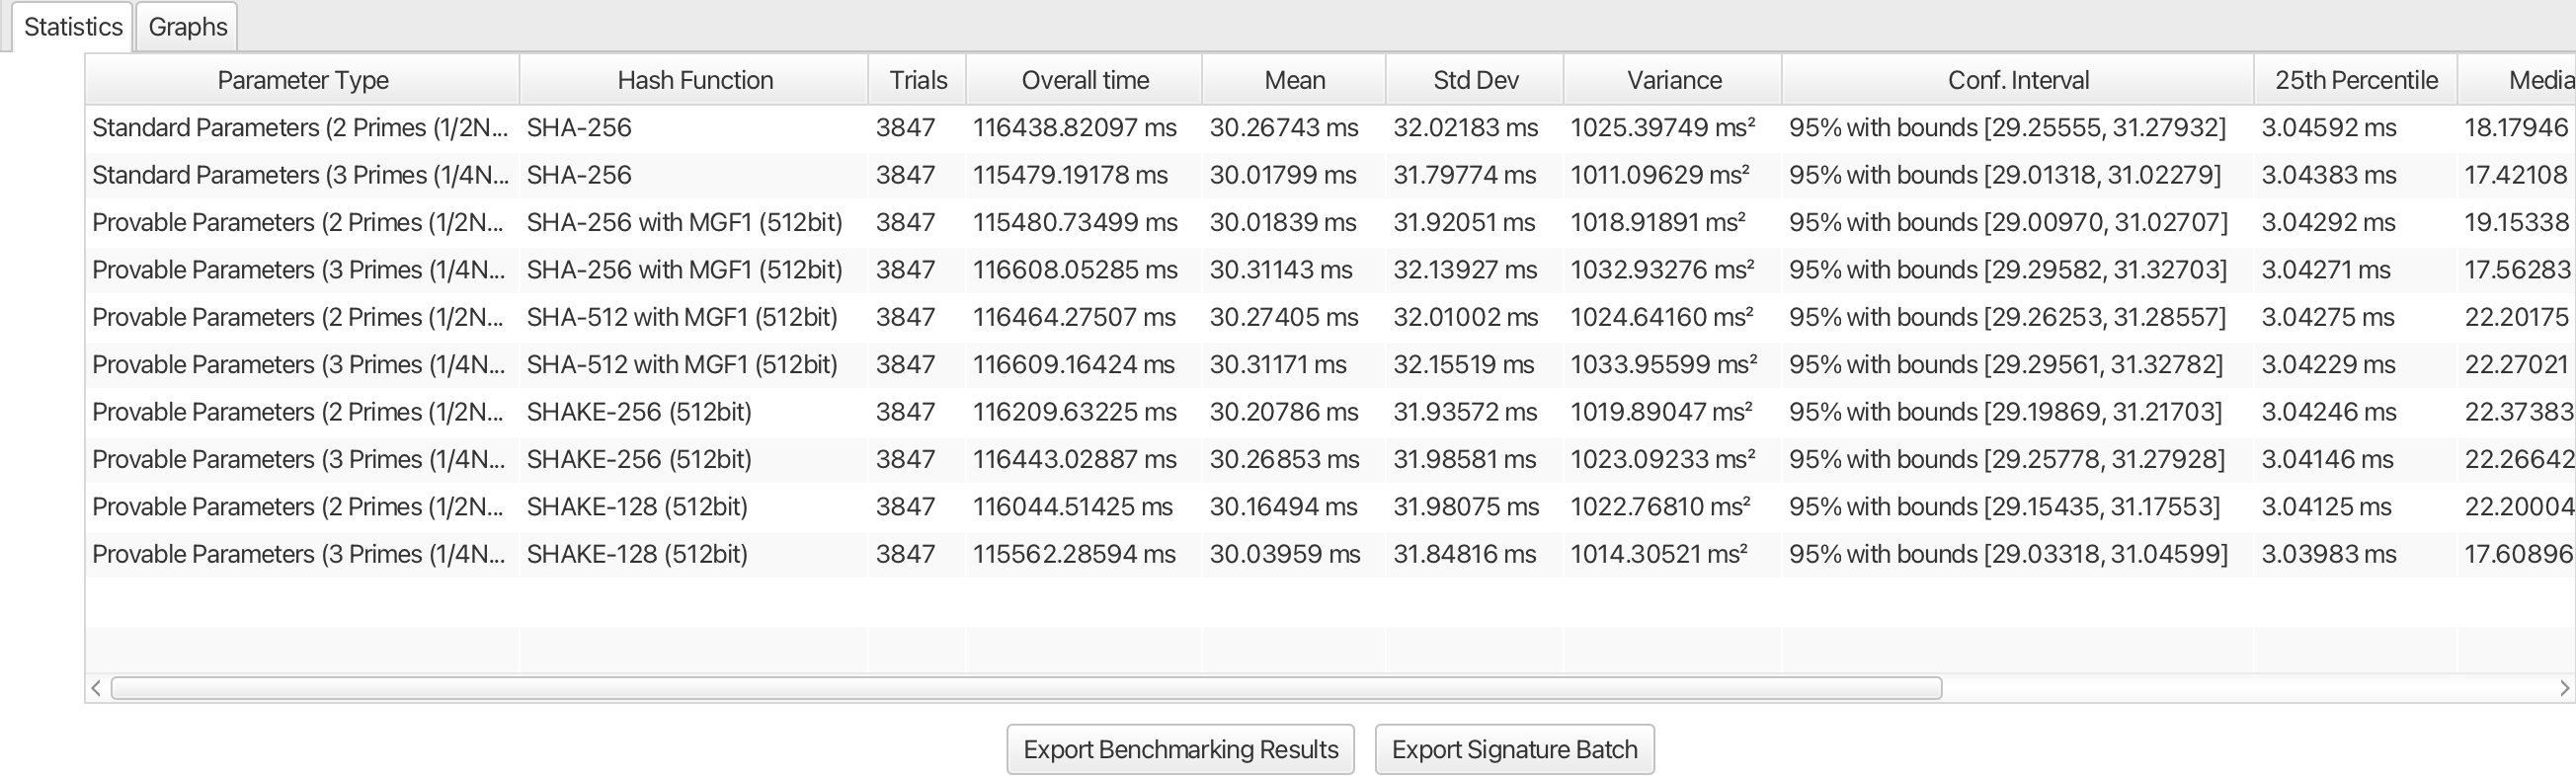
\includegraphics[width=\textwidth]{main_pictures/ansi/ansi_sign_1024bit_table1_1.png}} 
        \fbox{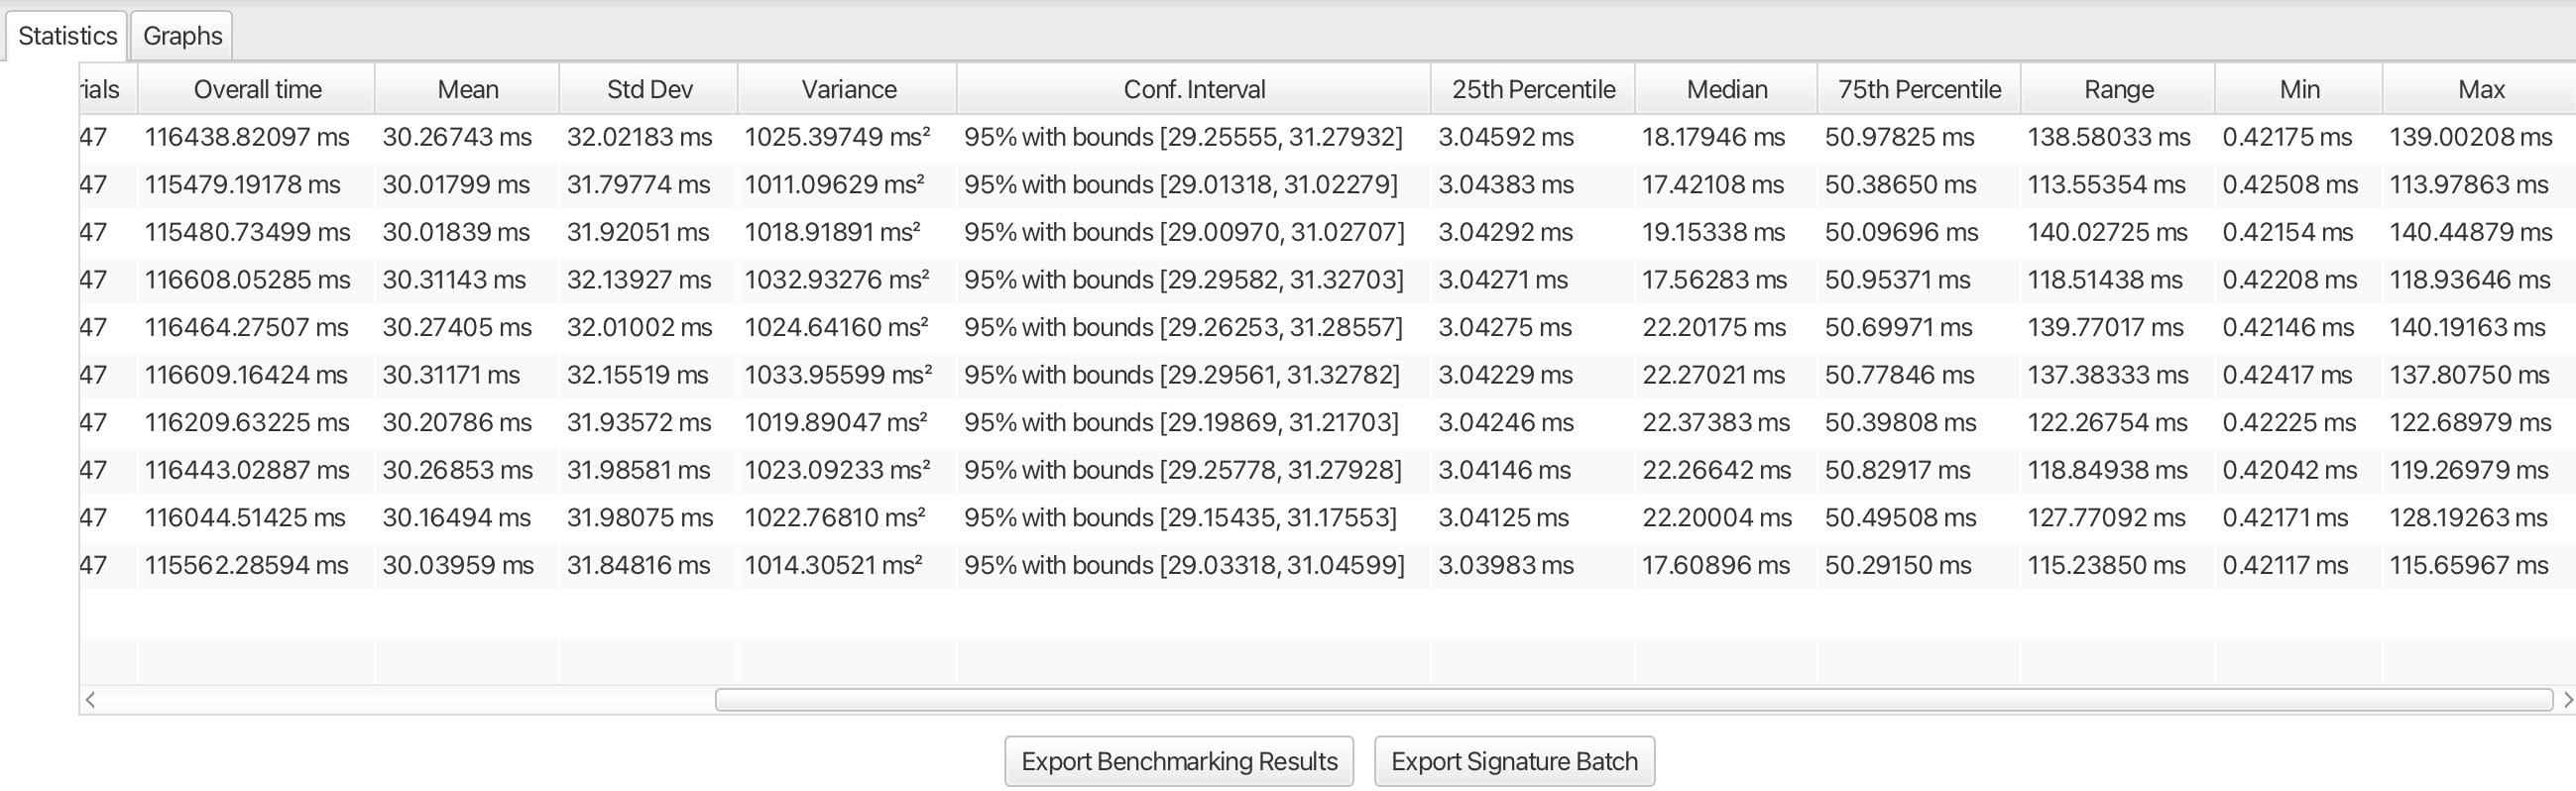
\includegraphics[width=\textwidth]{main_pictures/ansi/ansi_sign_1024bit_table2_1.png}}
    \end{minipage}
            \label{ansi_sign_1024bit_table}
  \end{figure}
  
\begin{figure}[H]
    \centering % Center the images
     \caption{Instantiation of ANSI X9.31 rDSA with standard vs provably secure parameters (2048-bit Key Size) for signature creation}
    % First image in a minipage
    \begin{minipage}{\textwidth}
        \centering
        \fbox{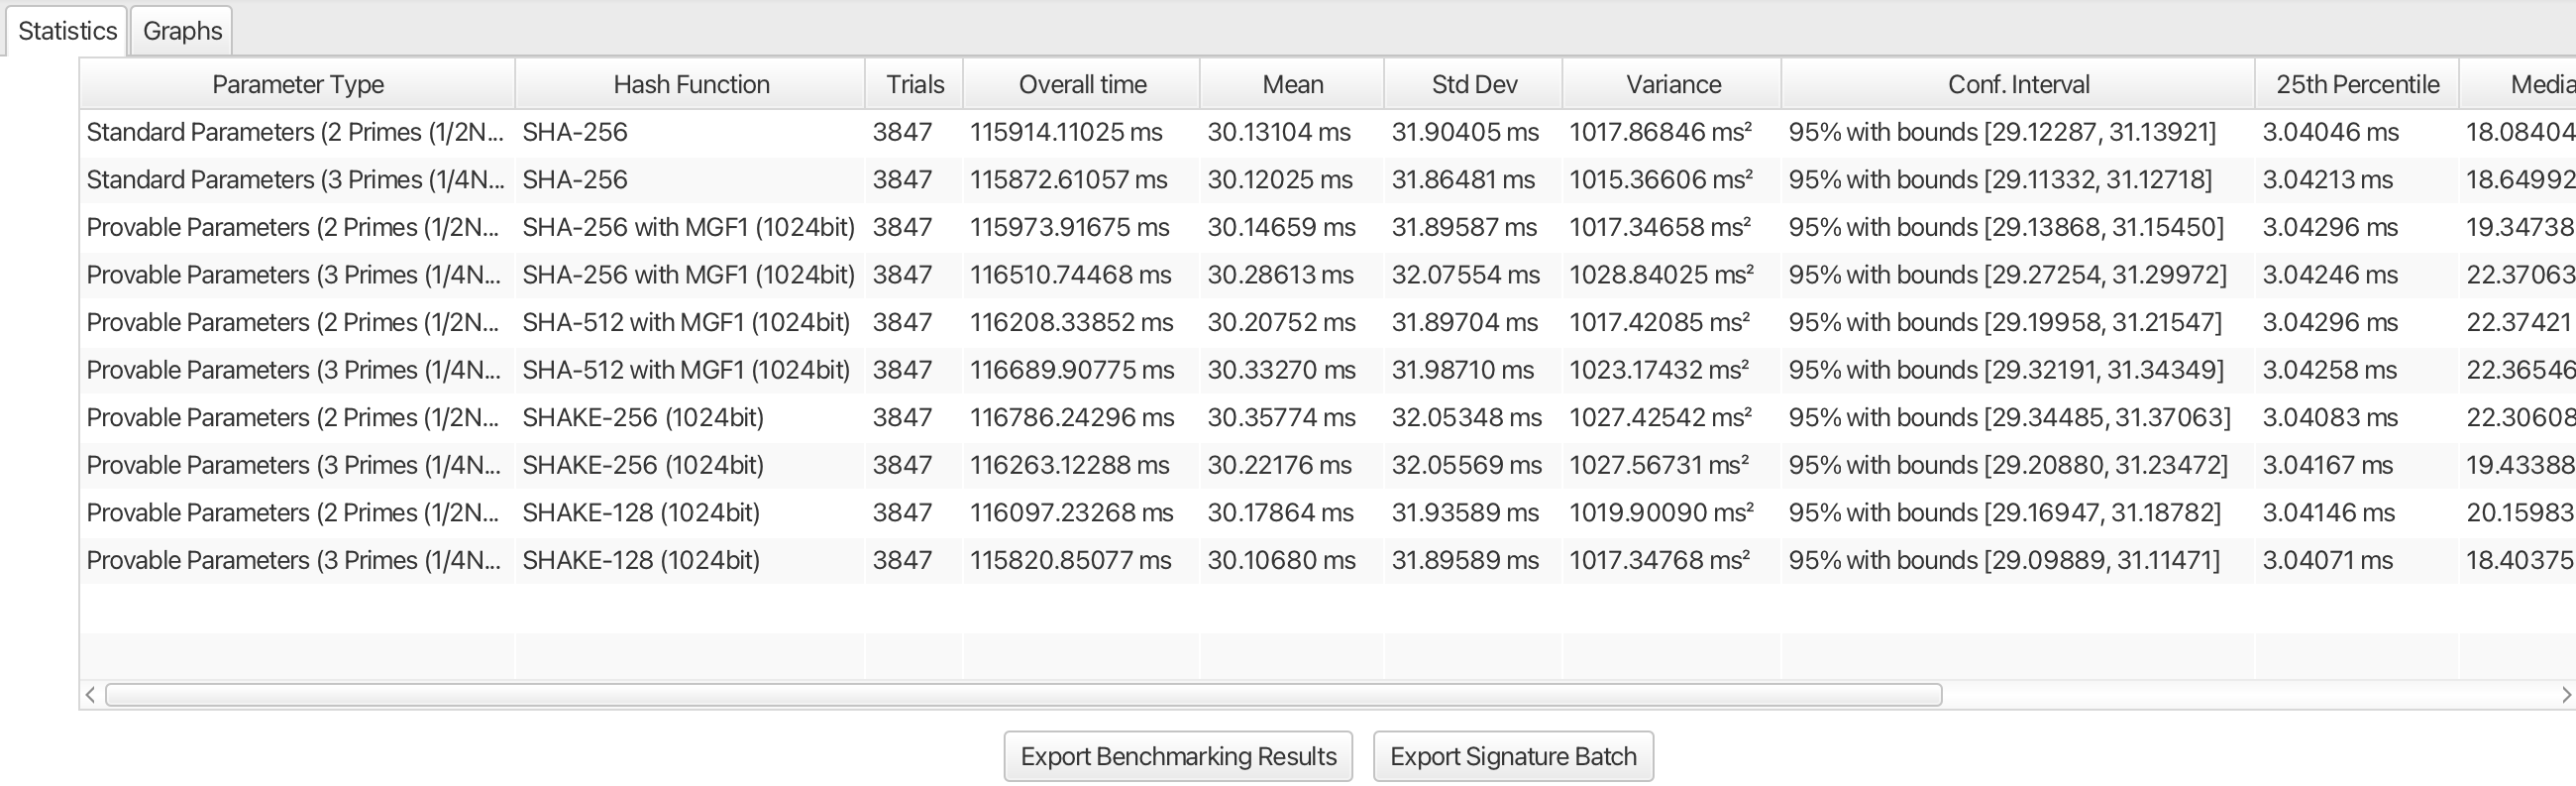
\includegraphics[width=\textwidth]{main_pictures/ansi/ansi_sign_2048bit_table1_1.png}} 
        \fbox{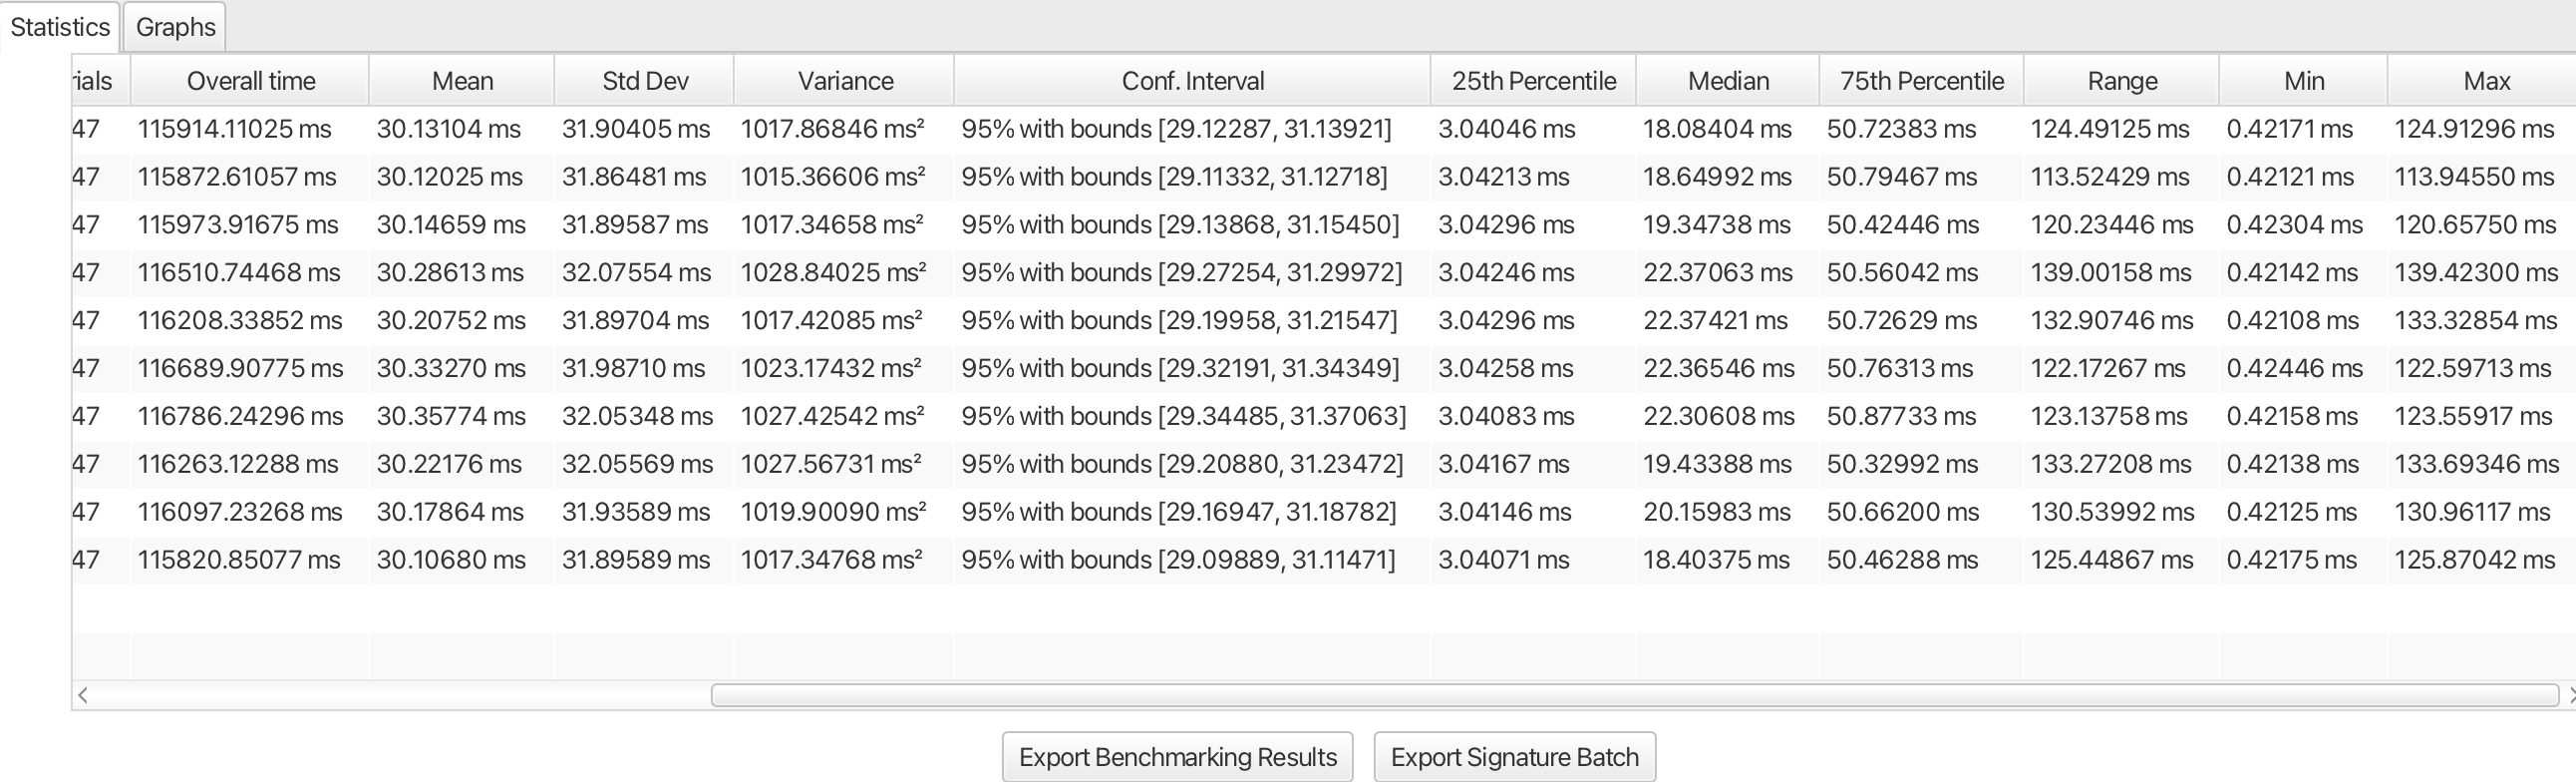
\includegraphics[width=\textwidth]{main_pictures/ansi/ansi_sign_2048bit_table2_1.png}}
    \end{minipage}
            \label{ansi_sign_2048bit_table}
  \end{figure}
  
\begin{figure}[H]
    \centering % Center the images
     \caption{Instantiation of ANSI X9.31 rDSA with standard vs provably secure parameters (3072-bit Key Size) for signature creation}
    % First image in a minipage
    \begin{minipage}{\textwidth}
        \centering
        \fbox{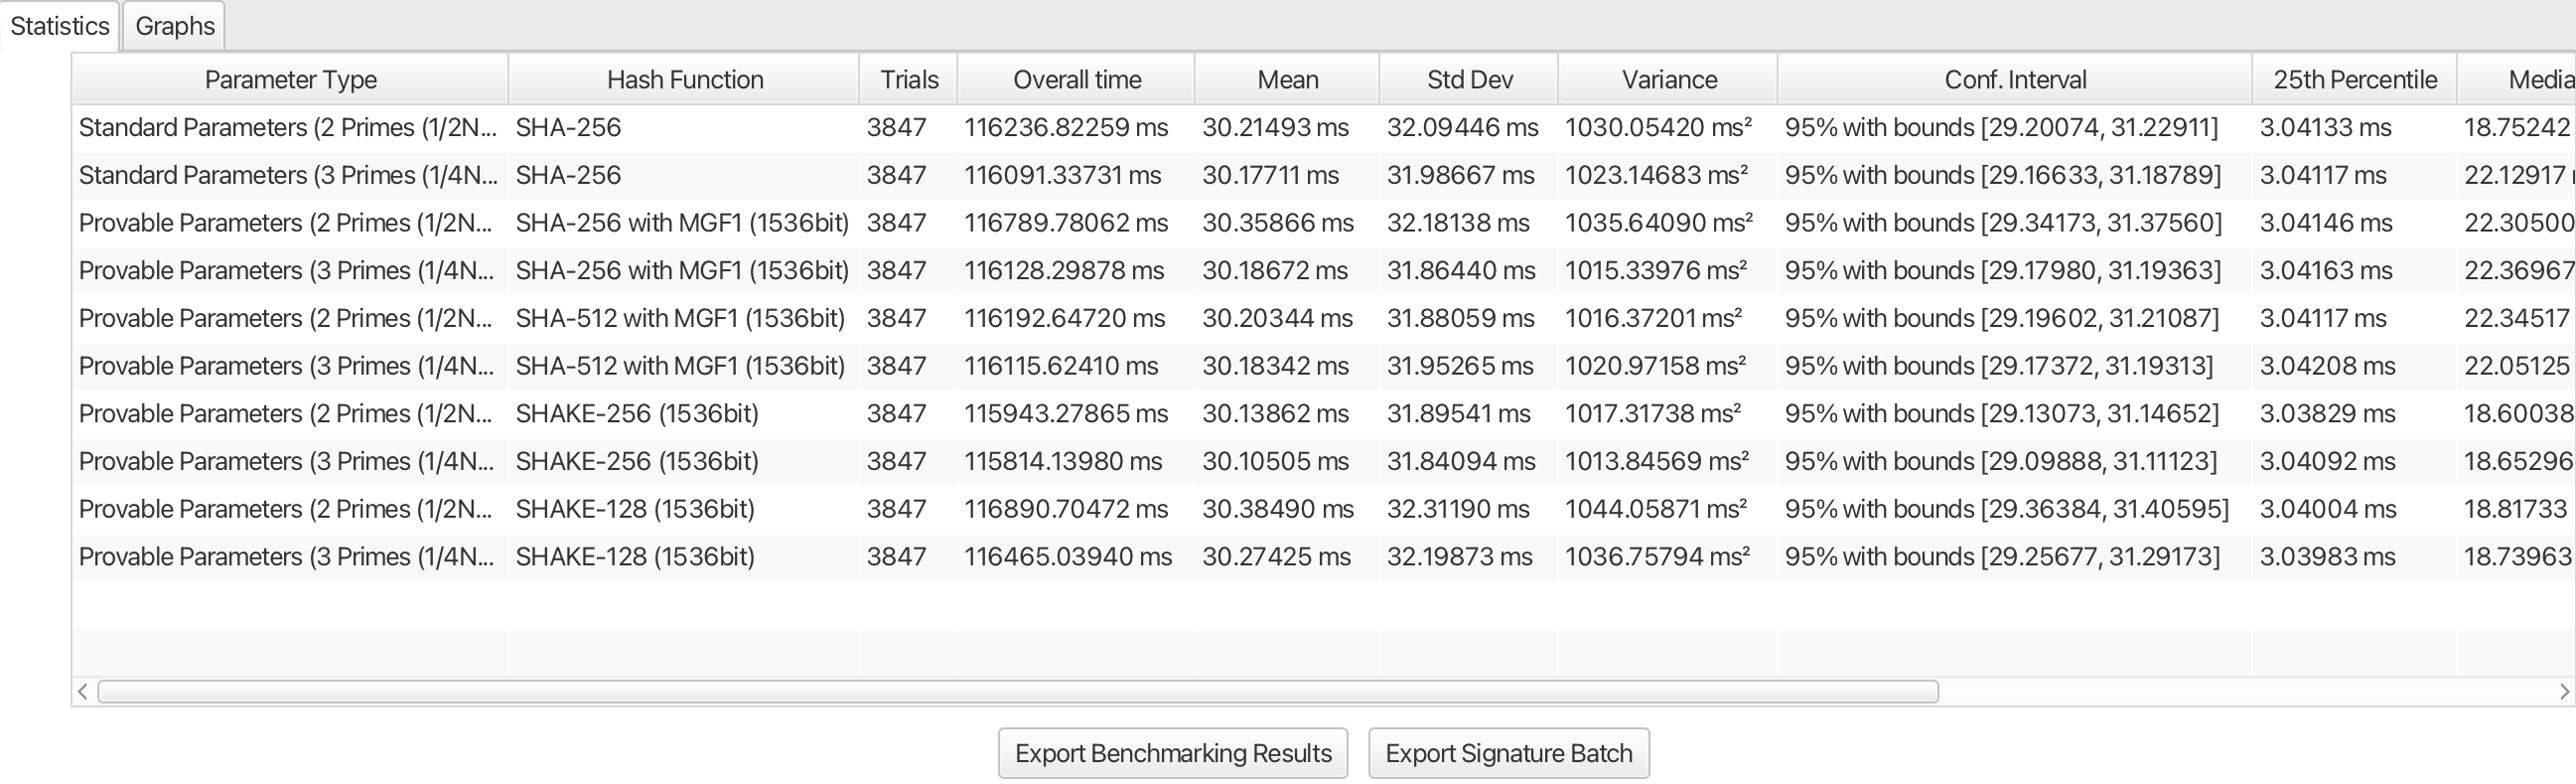
\includegraphics[width=\textwidth]{main_pictures/ansi/ansi_sign_3072bit_table1_1.png}} 
        \fbox{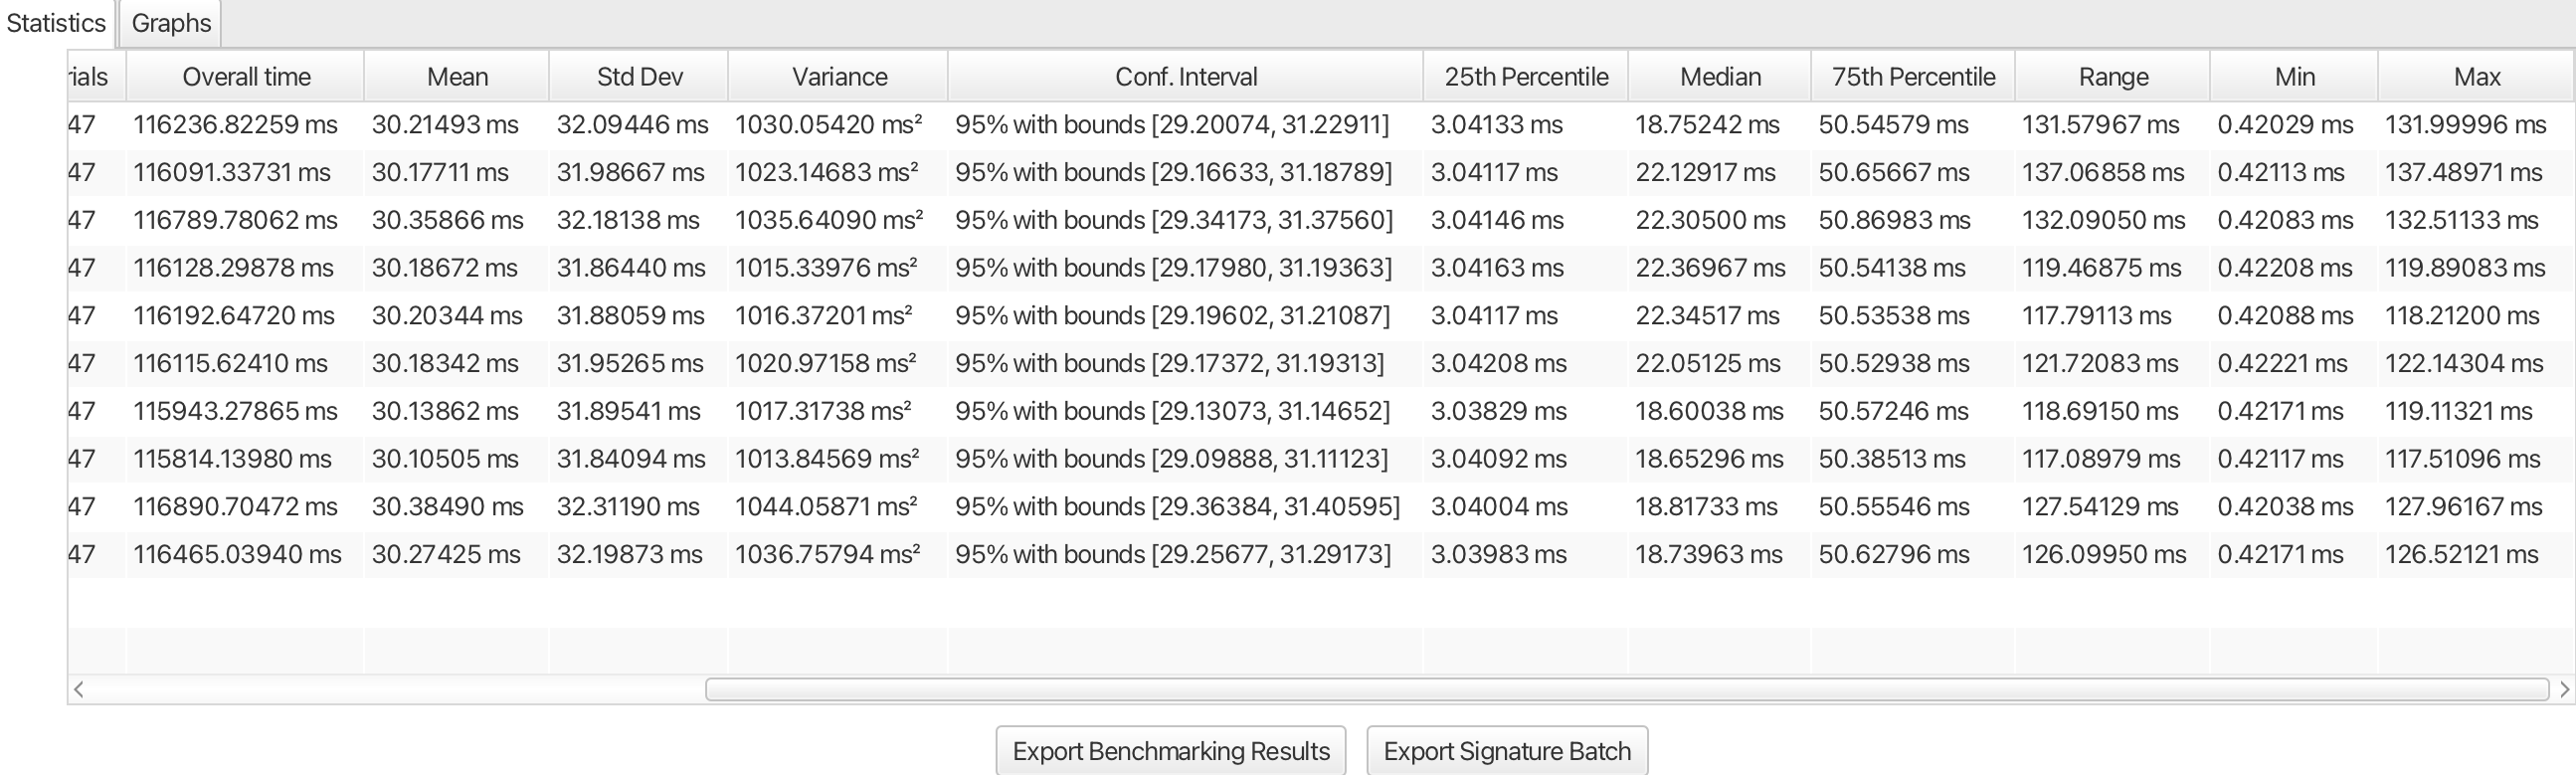
\includegraphics[width=\textwidth]{main_pictures/ansi/ansi_sign_3072bit_table2_1.png}}
    \end{minipage}
         \label{ansi_sign_3072bit_table}
\end{figure}

\begin{figure}[H]
    \centering % Center the images
     \caption{Instantiation of ANSI X9.31 rDSA with standard vs provably secure parameters (4096-bit Key Size) for signature creation}
    % First image in a minipage
    \begin{minipage}{\textwidth}
        \centering
        \fbox{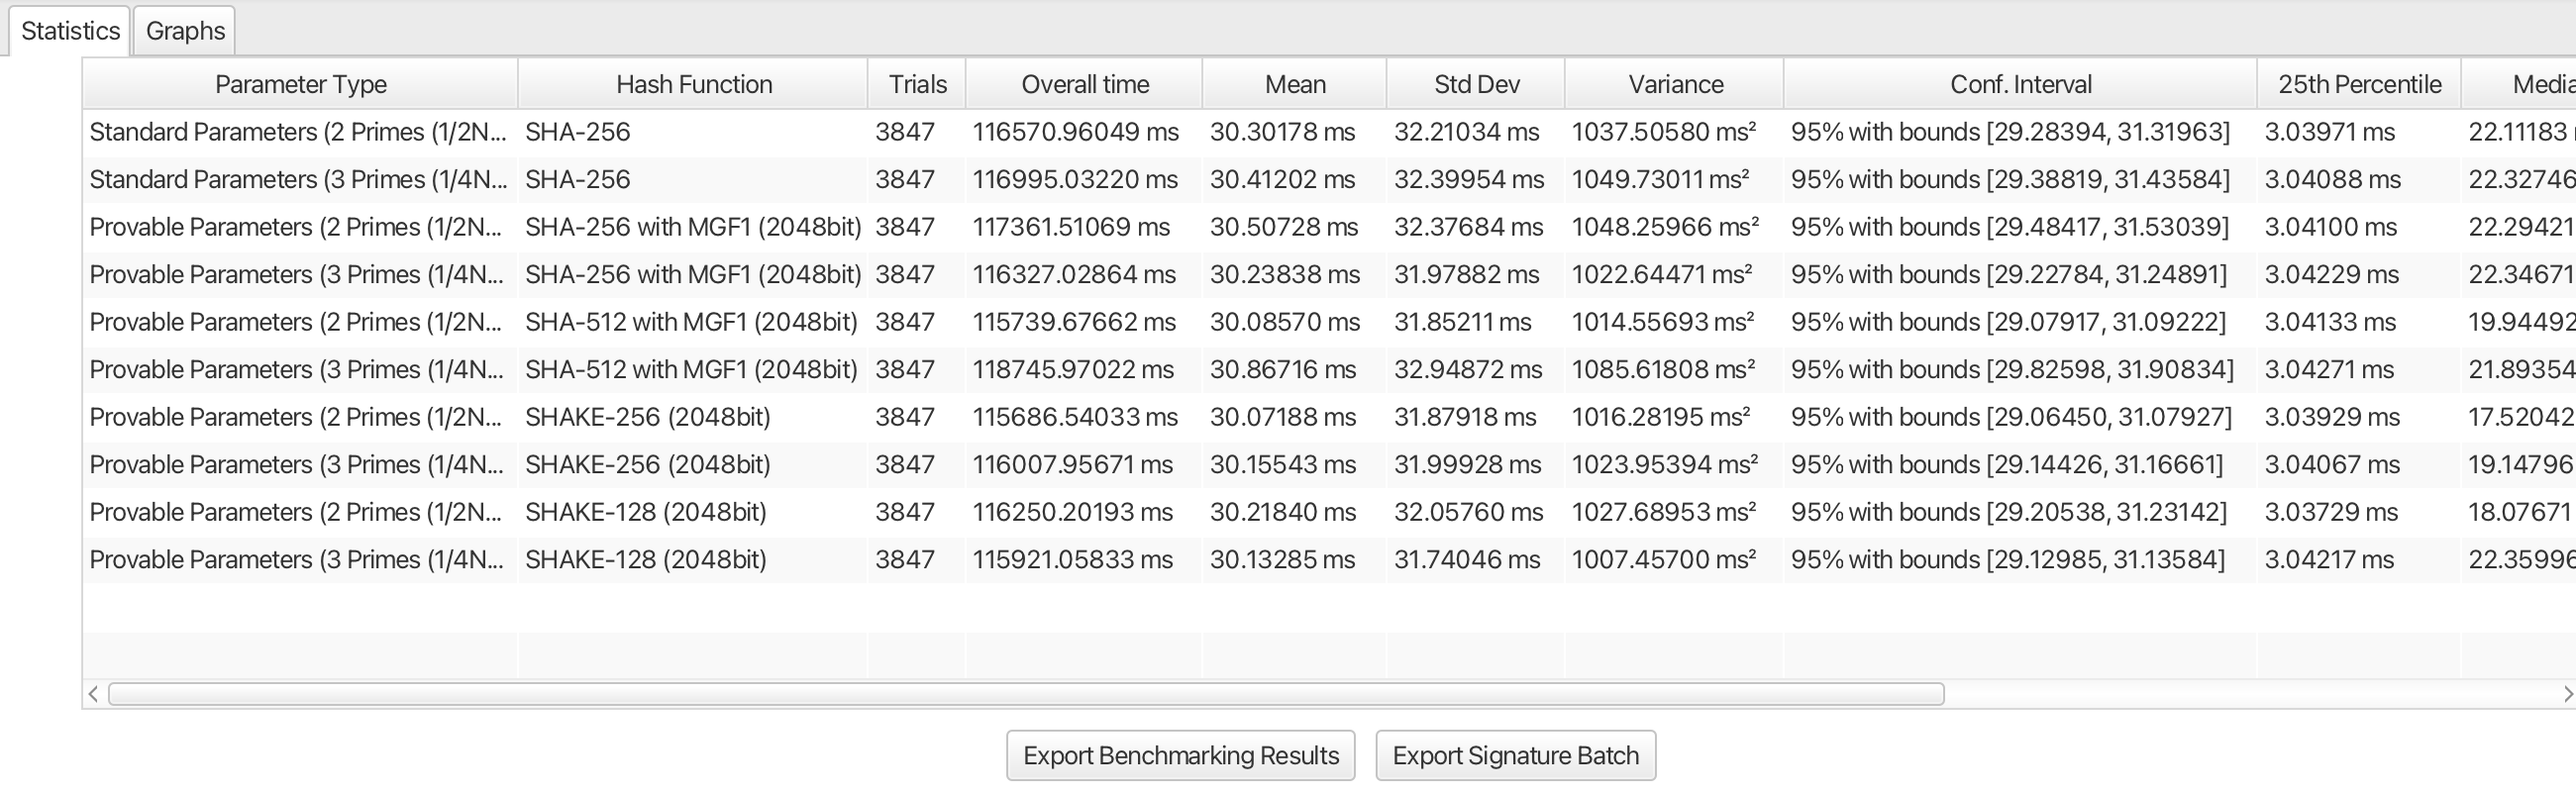
\includegraphics[width=\textwidth]{main_pictures/ansi/ansi_sign_4096bit_table1_1.png}} 
        \fbox{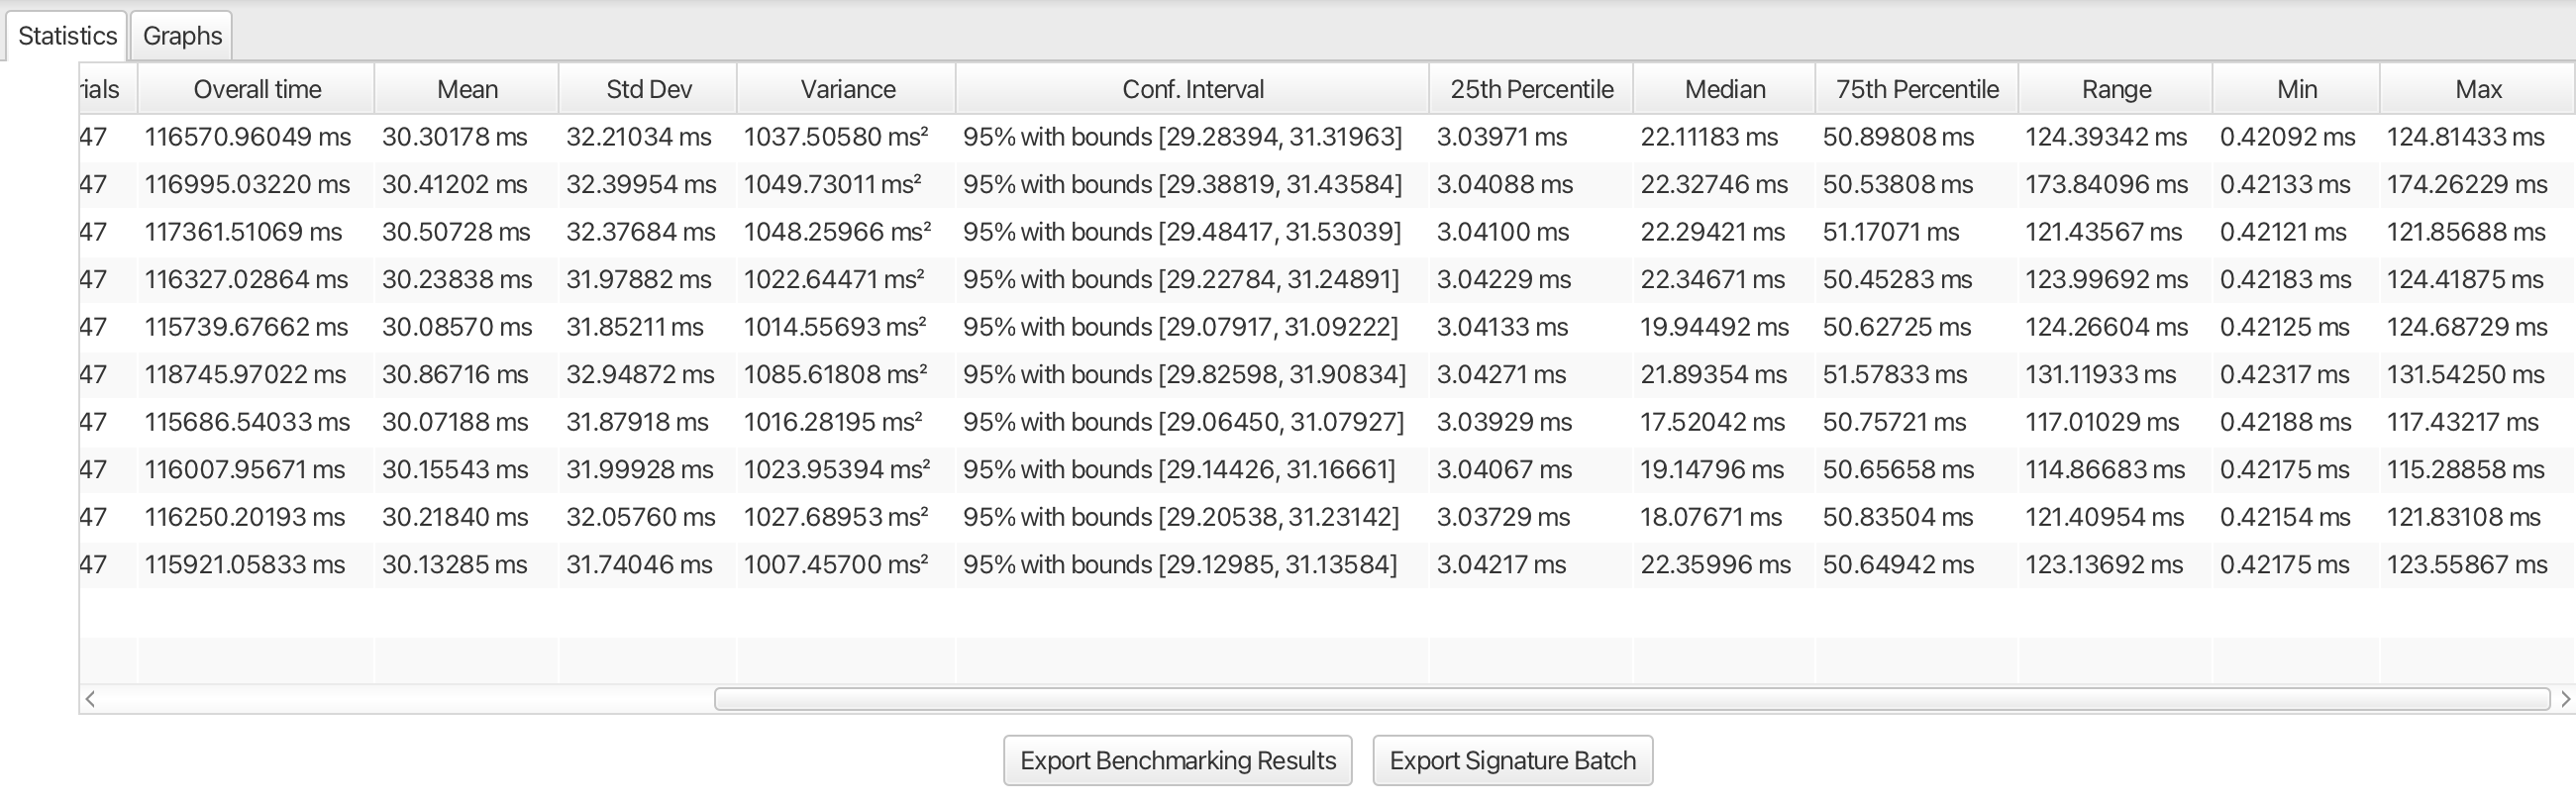
\includegraphics[width=\textwidth]{main_pictures/ansi/ansi_sign_4096bit_table2_1.png}}
    \end{minipage}
             \label{ansi_sign_4096bit_table}
\end{figure}

\begin{figure}[H]
    \centering % Center the images
     \caption{Instantiation of ANSI X9.31 rDSA with standard vs provably secure parameters (5120-bit Key Size) for signature creation}
    % First image in a minipage
    \begin{minipage}{\textwidth}
        \centering
        \fbox{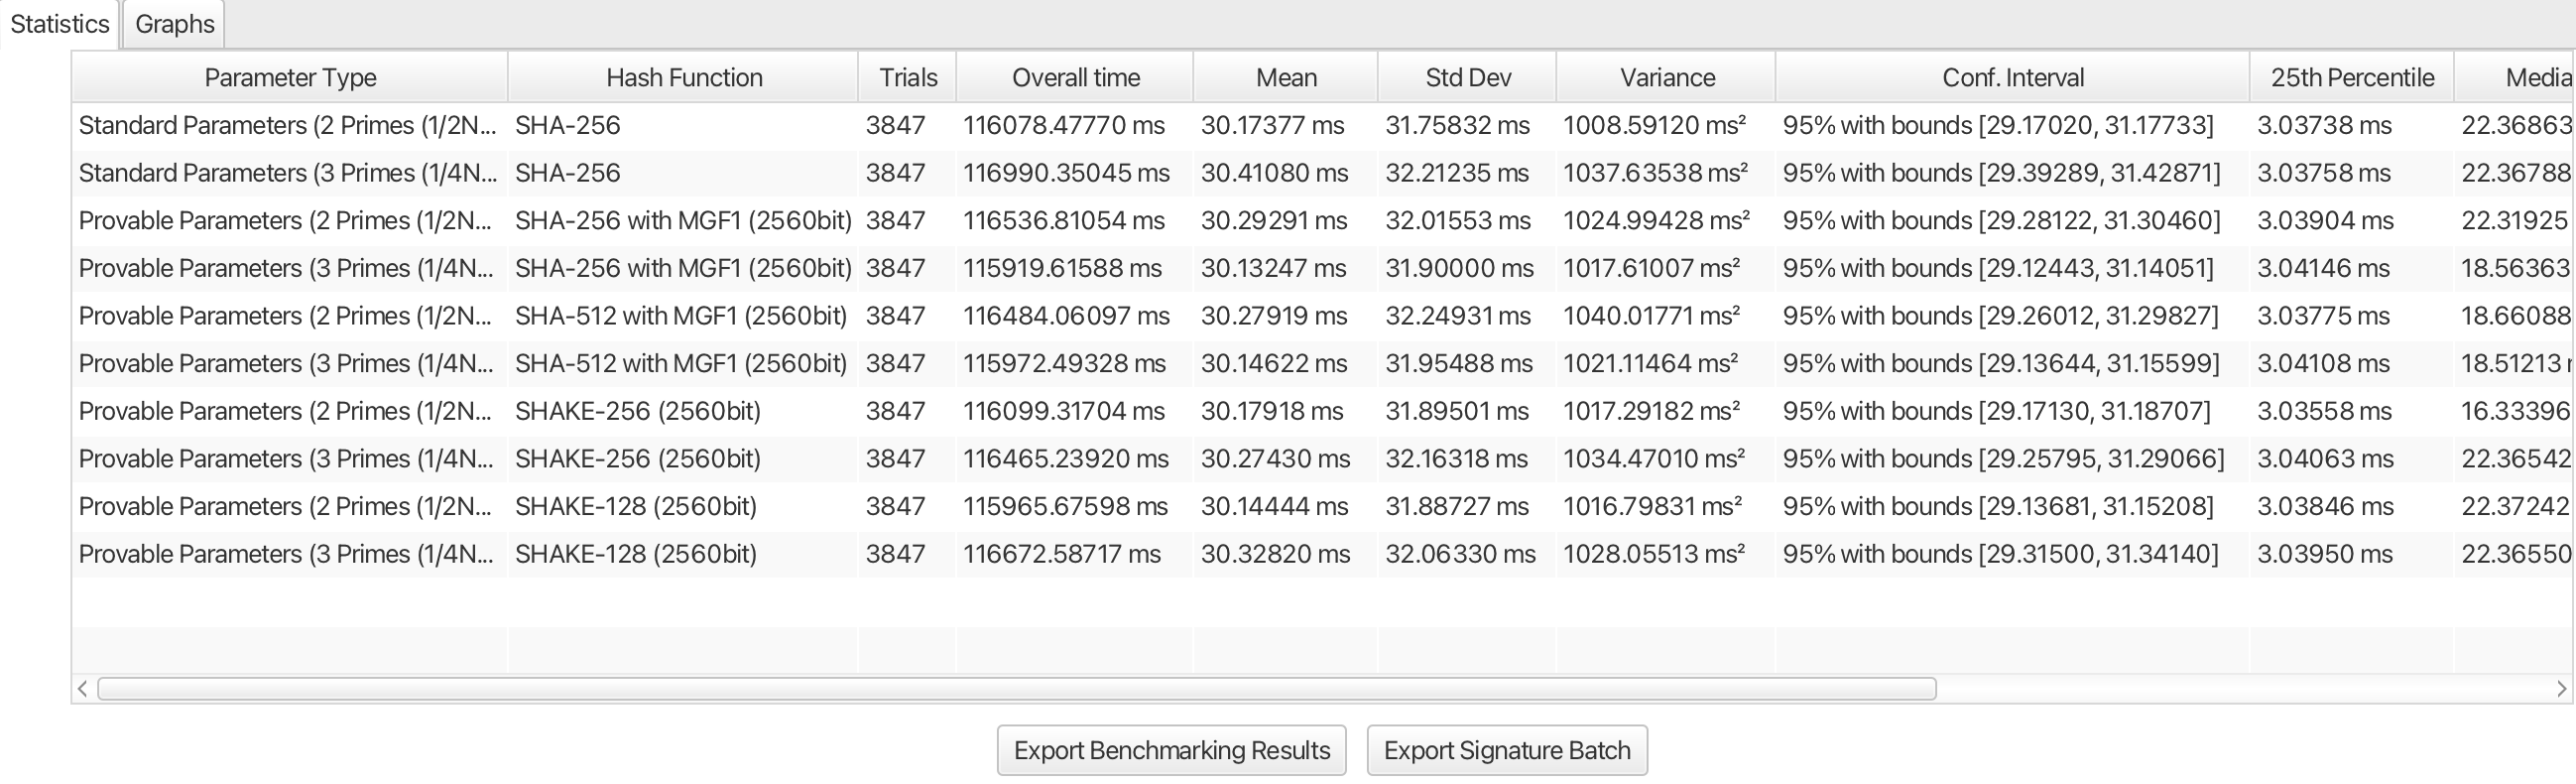
\includegraphics[width=\textwidth]{main_pictures/ansi/ansi_sign_5120bit_table1_1.png}} 
        \fbox{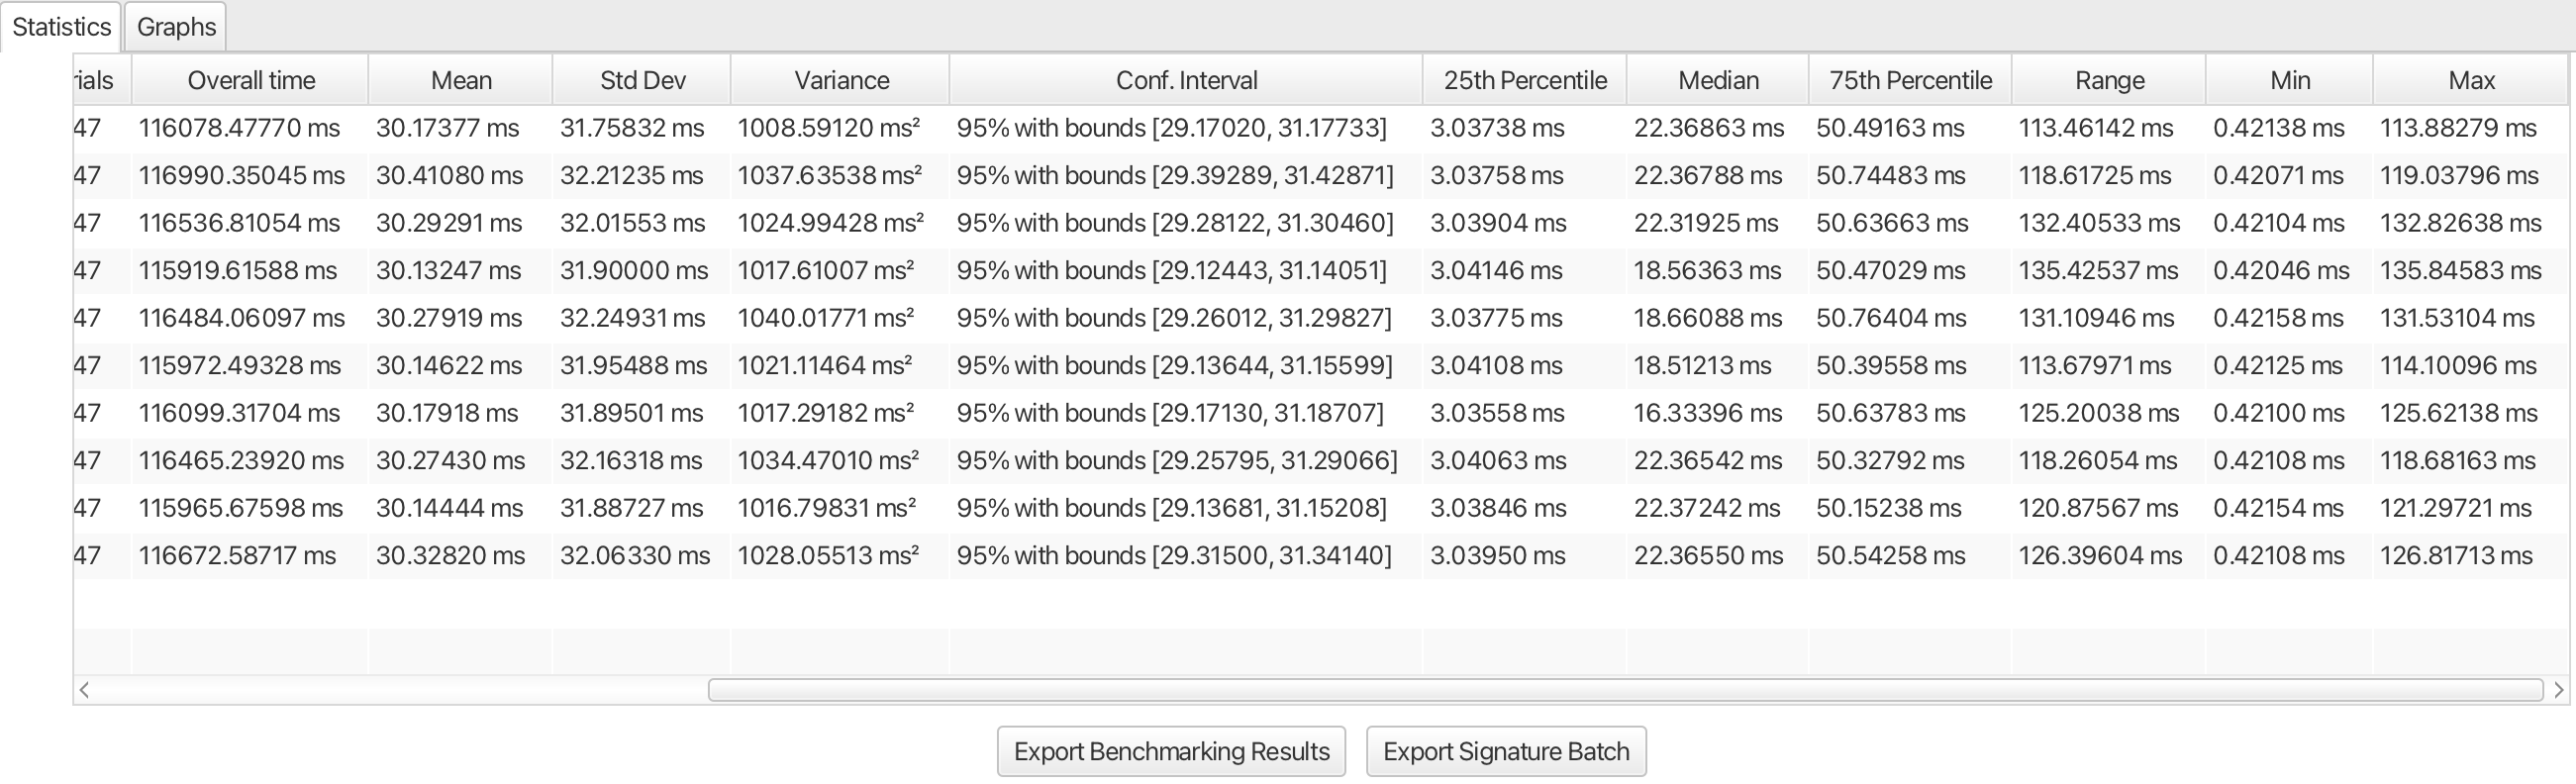
\includegraphics[width=\textwidth]{main_pictures/ansi/ansi_sign_5120bit_table2_1.png}}
    \end{minipage}
     \label{ansi_sign_5120bit_table}
\end{figure}

\begin{figure}[H]
    \centering % Center the images
     \caption{Instantiation of ANSI X9.31 rDSA with standard vs provably secure parameters (6144-bit Key Size) for signature creation}
    % First image in a minipage
    \begin{minipage}{\textwidth}
        \centering
        \fbox{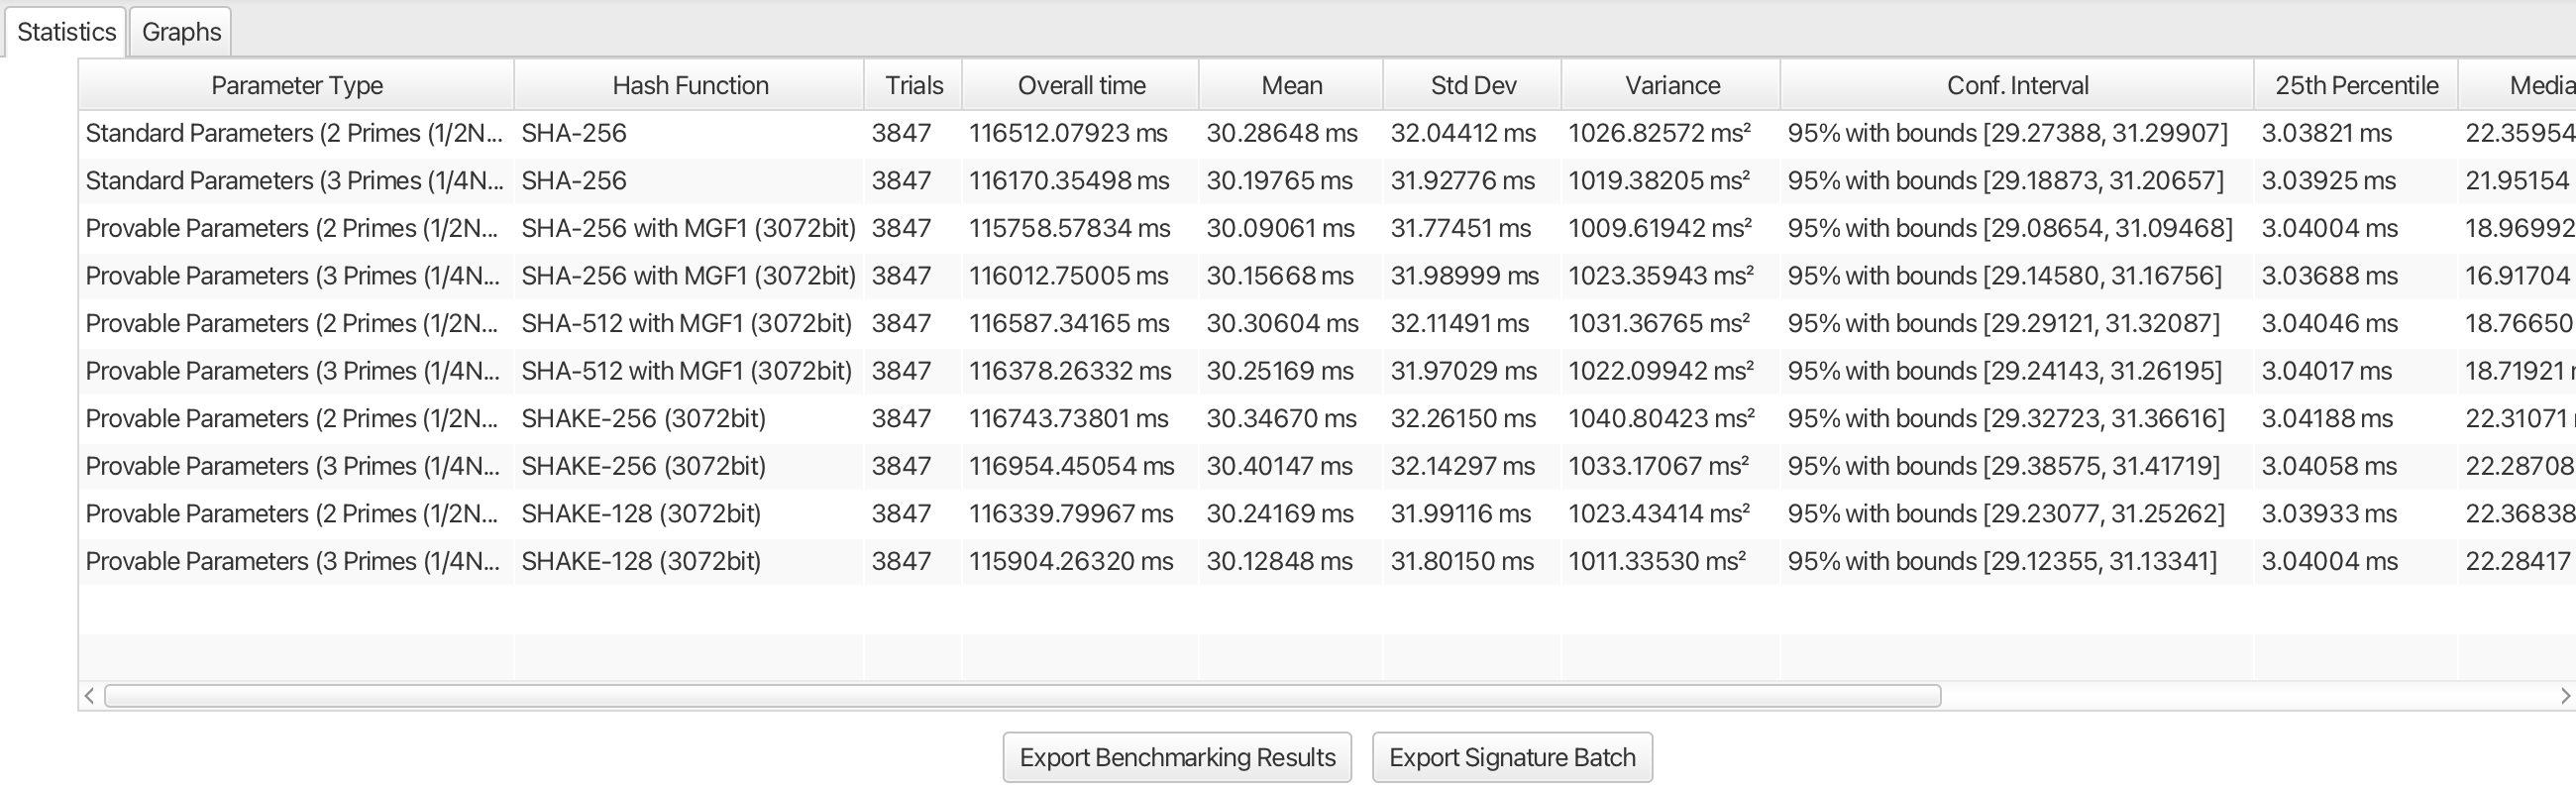
\includegraphics[width=\textwidth]{main_pictures/ansi/ansi_sign_6144bit_table1_1.png}} 
        \fbox{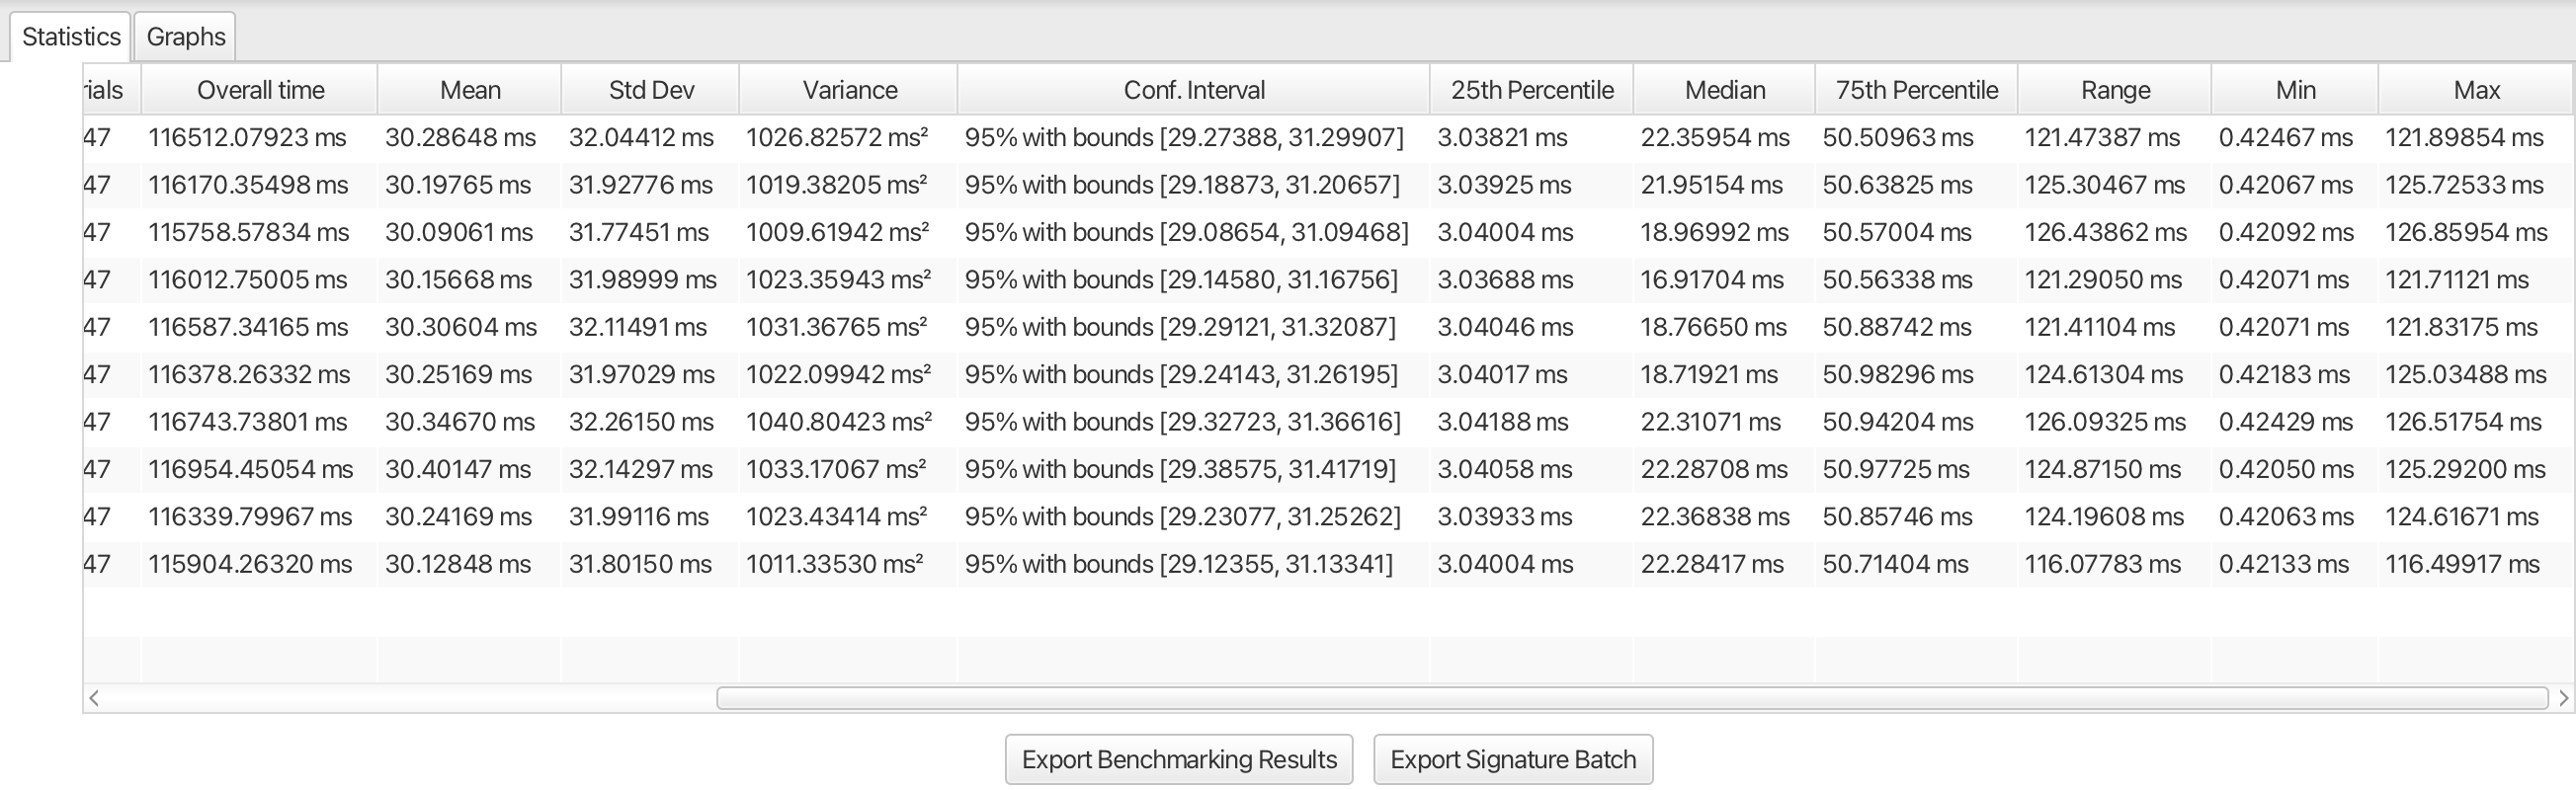
\includegraphics[width=\textwidth]{main_pictures/ansi/ansi_sign_6144bit_table2_1.png}}
    \end{minipage}
         \label{ansi_sign_6144bit_table}
\end{figure}

\begin{comment}
\textbf{1024-bit Key Size (\ref{ansi_sign_1024bit_table})}:

For the 1024-bit key size, the analysis of standard and provably secure parameters shows nuanced differences. In standard parameters using two primes, SHA-256 has a mean time of 30.26743 ms. Shifting to provably secure parameters with two primes, the mean times span from 30.01839 ms to 30.31171 ms for different hash functions, indicating a performance variation up to approximately 0.82\%, manifesting as either increases or decreases. For configurations using three primes, the standard parameter's mean time for SHA-256 is 30.01799 ms, compared to a range of 30.03959 ms to 30.31171 ms for provably secure parameters, reflecting a variation up to about 0.98\%.

\textbf{2048-bit Key Size (\ref{ansi_sign_2048bit_table})}:

At the 2048-bit key size, standard parameters with two primes show a mean time of 30.13104 ms. For provably secure parameters with two primes, the times range between 30.14659 ms and 30.35774 ms. This exhibits a performance difference of up to 0.75\%. In three-prime configurations, the standard parameter mean time is 30.12025 ms, while for provably secure parameters, the mean times vary from 30.10680 ms to 30.33270 ms, indicating a possible variation up to 0.70\%.

\textbf{3072-bit Key Size (\ref{ansi_sign_3072bit_table})}:

For the 3072-bit key size, the standard parameters with two primes yield a mean time of 30.21493 ms. In contrast, the mean times for provably secure parameters range from 30.13862 ms to 30.38490 ms, showing a performance difference of up to 0.82\%. With three primes, the standard mean time is 30.17711 ms, and for provably secure parameters, the range is from 30.10505 ms to 30.27425 ms, translating to a variation up to approximately 0.24\%.

\textbf{4096-bit Key Size (\ref{ansi_sign_4096bit_table})}:

At the 4096-bit key size, using standard parameters with two primes, the mean time for SHA-256 is 30.30178 ms. For provably secure parameters, the mean times span from 30.08570 ms to 30.50728 ms across various hash functions, indicating a performance change up to 1.39\%, either decreasing or increasing. With three primes, standard parameters yield a mean time of 30.41202 ms, compared to provably secure parameters ranging from 30.13285 ms to 30.86716 ms, showing a variance up to 1.49\%.

\textbf{5120-bit Key Size (\ref{ansi_sign_5120bit_table})}:

For the 5120-bit key size, the standard parameters with two primes indicate a mean time of 30.17377 ms for SHA-256. Switching to provably secure parameters, the range of mean times is from 30.13247 ms to 30.29291 ms, reflecting a performance variation of up to 0.57\%. In scenarios with three primes, the standard parameters show a mean time of 30.41080 ms, while provably secure parameters vary from 30.14444 ms to 30.32820 ms, showing a potential performance change of up to 0.88\%.

\textbf{6144-bit Key Size (\ref{ansi_sign_6144bit_table})}:

At the 6144-bit key size, standard parameters using two primes give a mean time of 30.28648 ms for SHA-256. In comparison, provably secure parameters yield mean times between 30.09061 ms and 30.34670 ms, demonstrating a variation up to approximately 0.65\%. For configurations with three primes, the standard mean time is 30.19765 ms, and for provably secure parameters, the range is 30.12848 ms to 30.40147 ms, indicating a performance variation of up to 0.91\%.

\end{comment}

Benchmarking across all key sizes for ANSI X9.31 rDSA signature creation reveals a consistent trend. With standard parameters using two primes, SHA-256 mean times range from 30.13104 ms to 30.41202 ms. For provably secure parameters with two primes, the mean times across different hash functions vary from 30.08570 ms to 30.50728 ms, demonstrating a performance variation of up to 1.39\%. With three primes, standard parameters yield mean times from 30.10680 ms to 30.41080 ms, while for provably secure parameters, the range is from 30.10680 ms to 30.86716 ms, indicating a potential variation of up to 1.49\% across all key sizes.


These results align with findings from PKCS\#1 v1.5 in that the difference between standard and provably secure parameters is negligible. The small fluctuations in performance times are likely inherent to computational processes and do not signify any significant statistical difference. Therefore it can be inferred that instantiation of ANSI X9.31 rDSA (for signature creation) with provably secure parameters does not introduce an overhead, and rather maintains effectiveness in line with standard parameters.




\section{Signature Creation Results (ISO/IEC 9796-2:2010 Signature Scheme 1)}

\begin{figure}[H]
    \centering % Center the images
     \caption{Instantiation of ISO/IEC 9796-2:2010 Signature Scheme 1 with standard vs provably secure parameters (1024-bit Key Size) for signature creation}
    % First image in a minipage
    \begin{minipage}{\textwidth}
        \centering
        \fbox{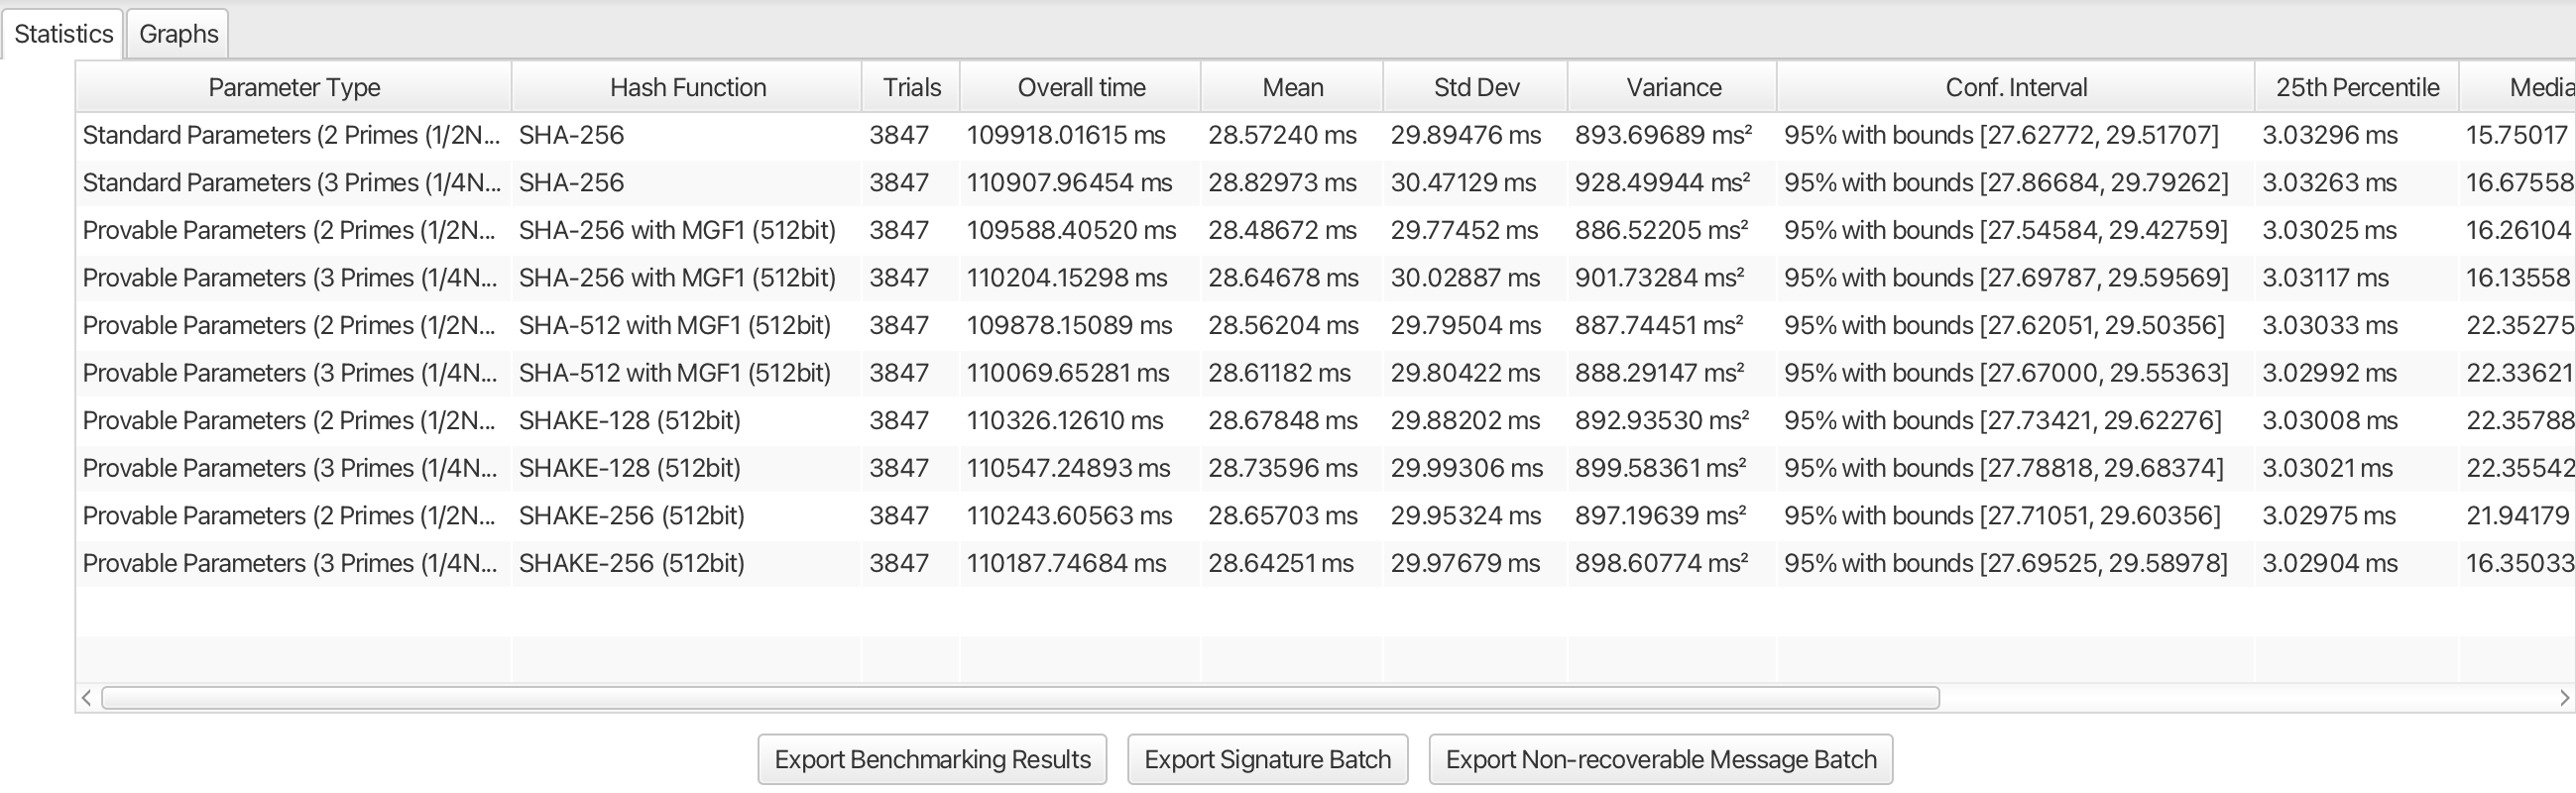
\includegraphics[width=\textwidth]{main_pictures/iso/iso_sign_1024bit_table1_1.png}} 
        \fbox{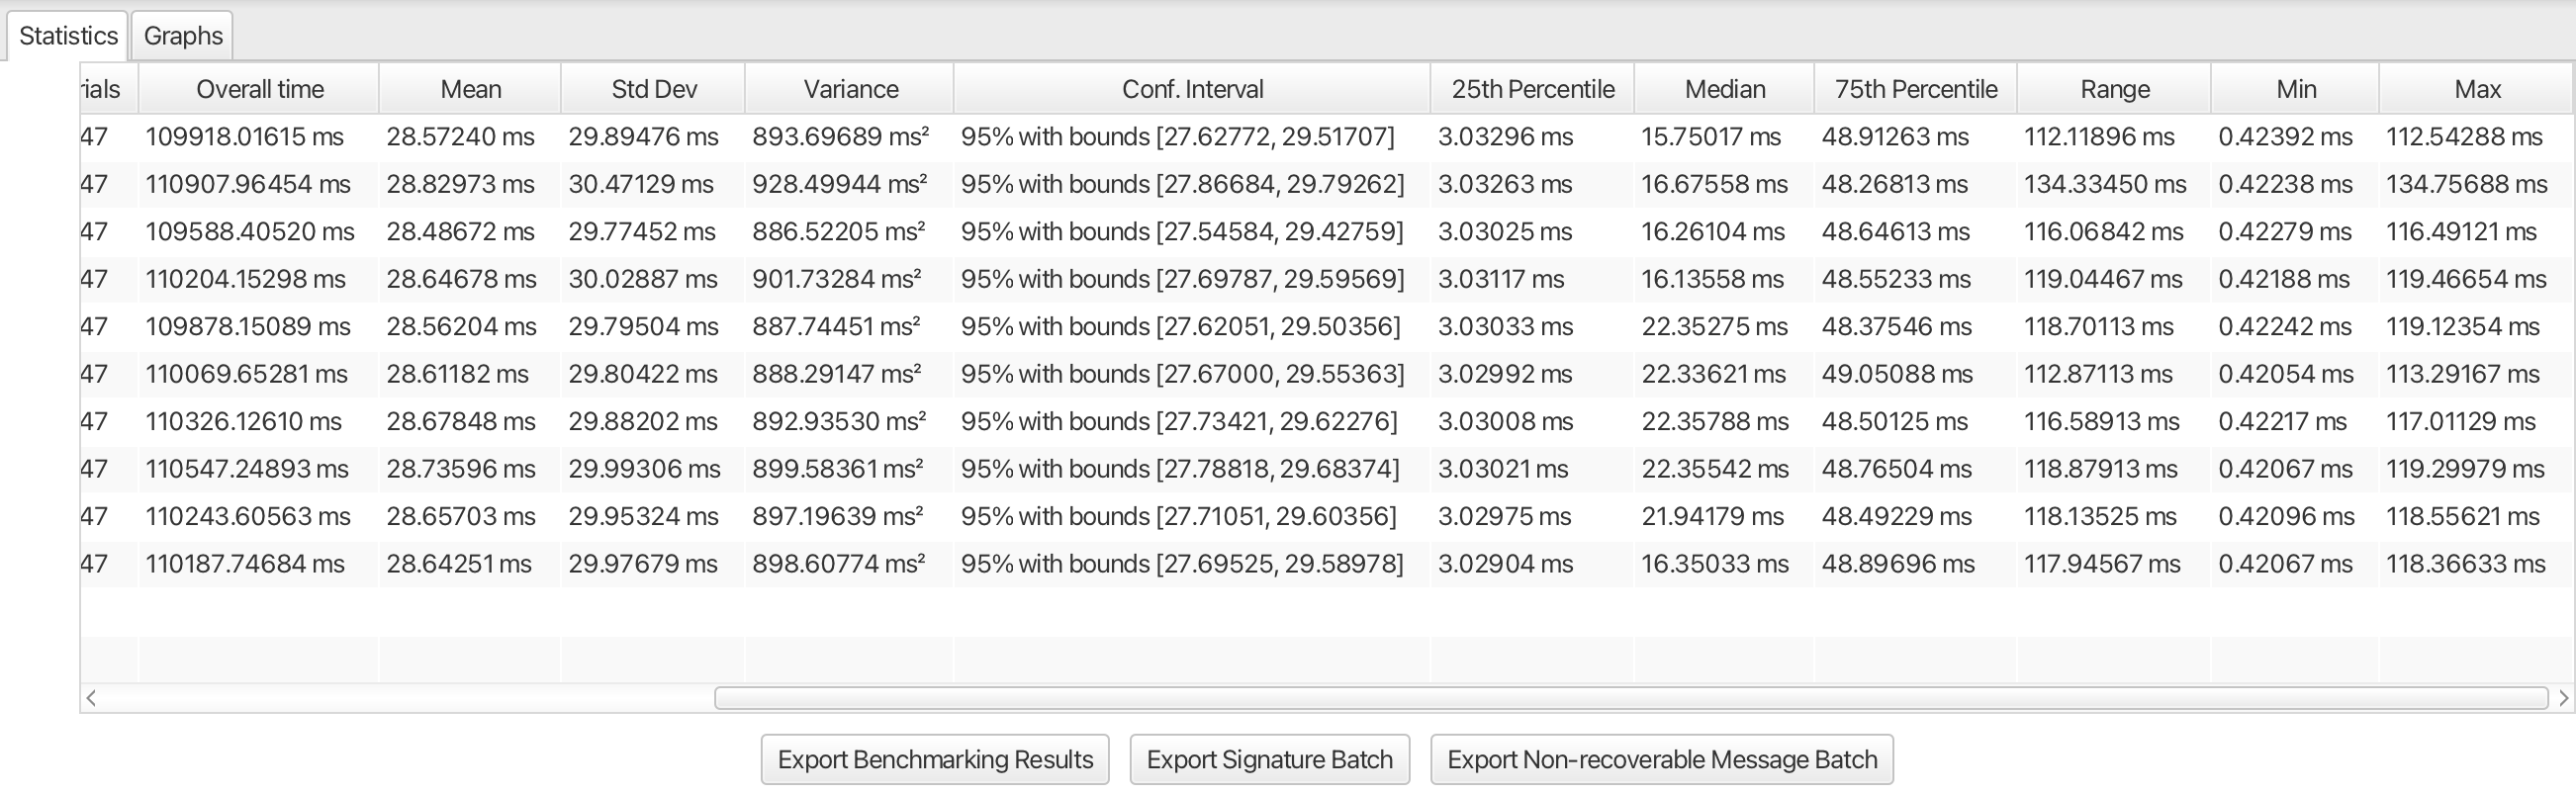
\includegraphics[width=\textwidth]{main_pictures/iso/iso_sign_1024bit_table2_1.png}}
    \end{minipage}
            \label{iso_sign_1024bit_table}
  \end{figure}
  
\begin{figure}[H]
    \centering % Center the images
     \caption{Instantiation of ISO/IEC 9796-2:2010 Signature Scheme 1 with standard vs provably secure parameters (2048-bit Key Size) for signature creation}
    % First image in a minipage
    \begin{minipage}{\textwidth}
        \centering
        \fbox{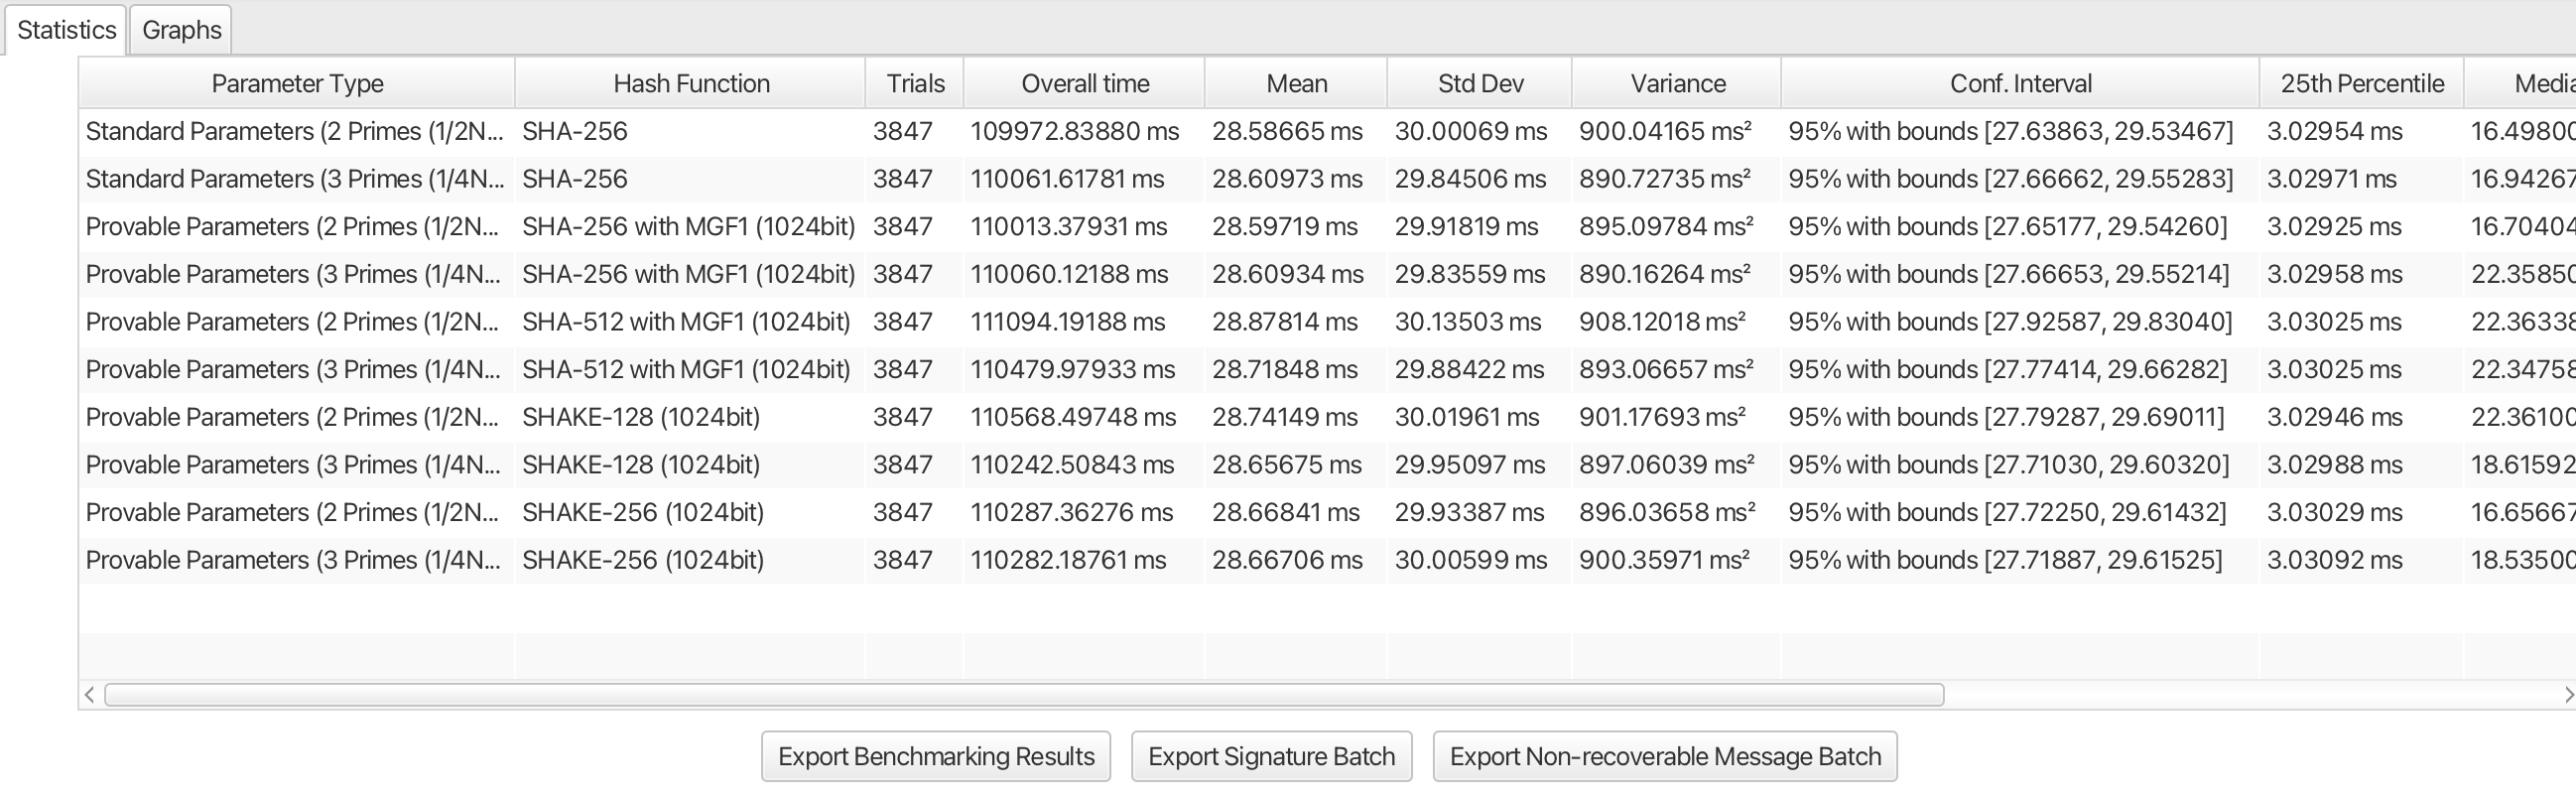
\includegraphics[width=\textwidth]{main_pictures/iso/iso_sign_2048bit_table1_1.png}} 
        \fbox{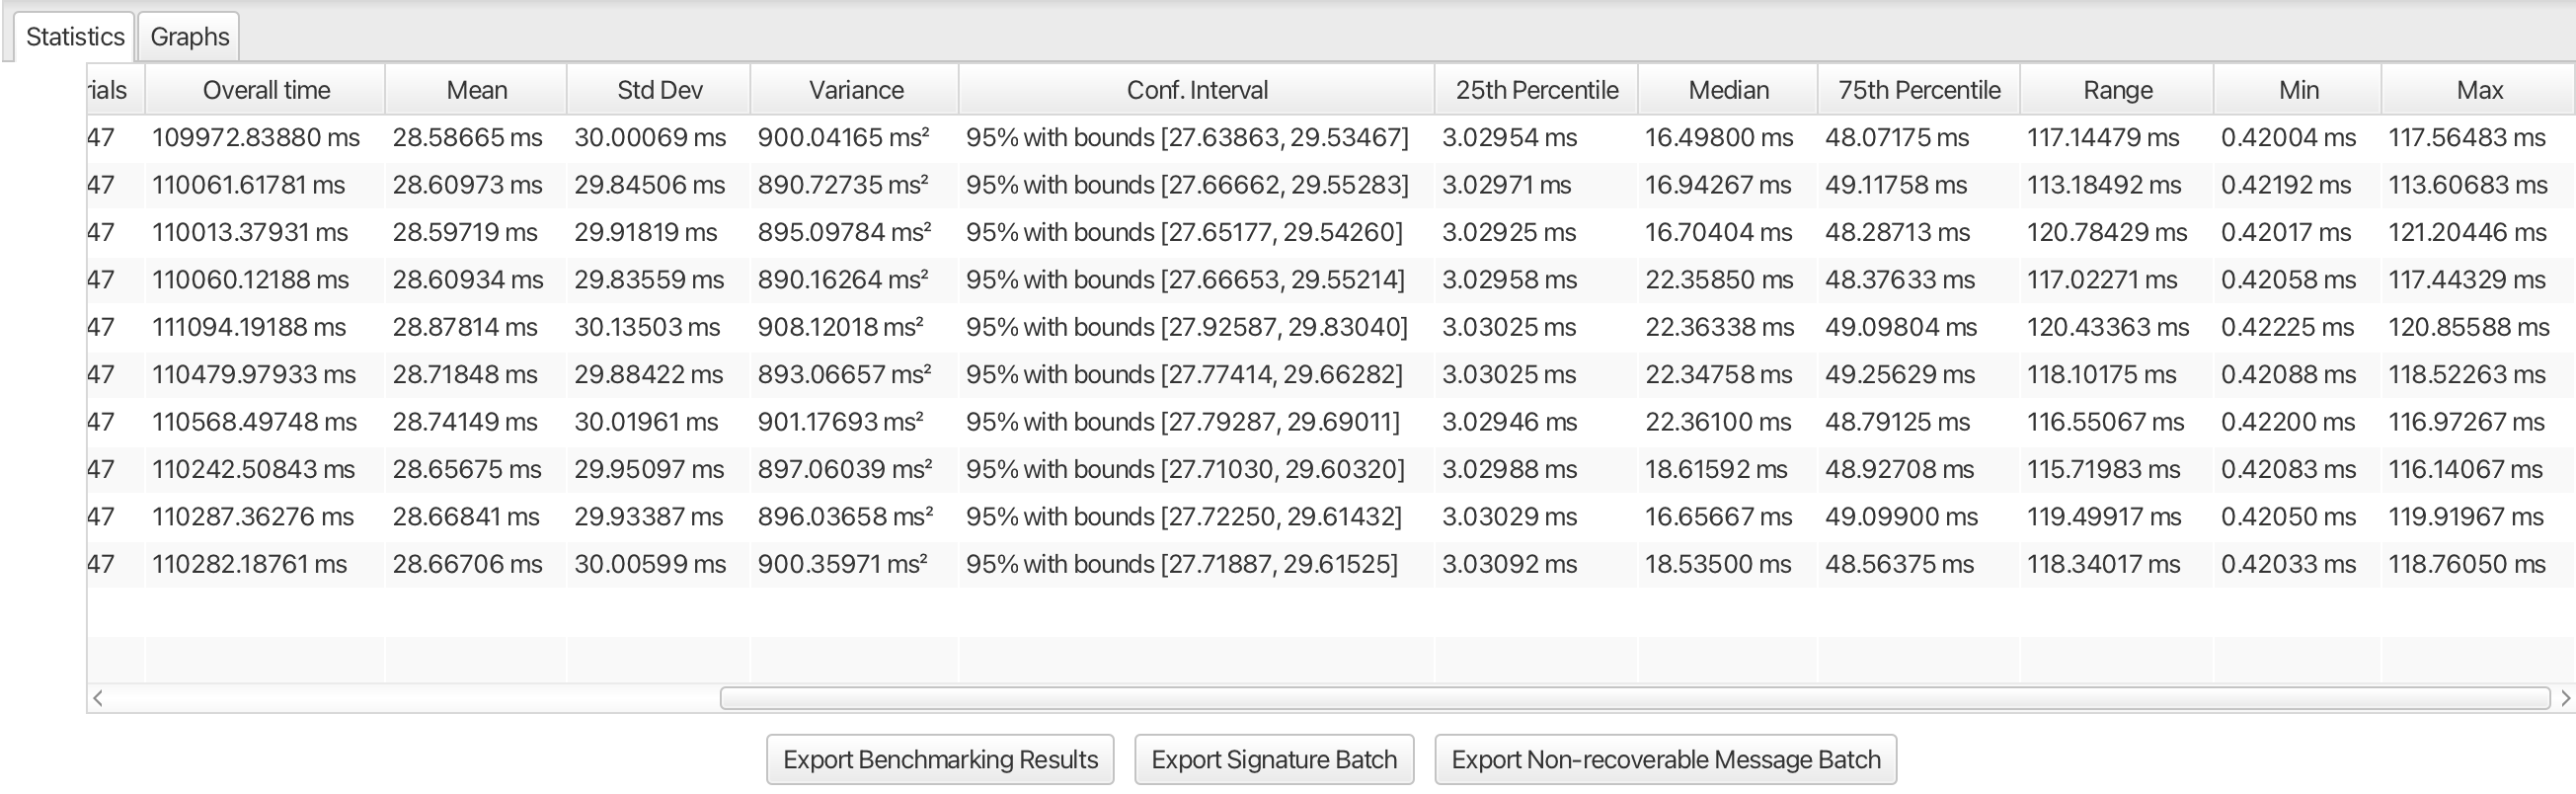
\includegraphics[width=\textwidth]{main_pictures/iso/iso_sign_2048bit_table2_1.png}}
    \end{minipage}
            \label{iso_sign_2048bit_table}
  \end{figure}
  
\begin{figure}[H]
    \centering % Center the images
     \caption{Instantiation of ISO/IEC 9796-2:2010 Signature Scheme 1 with standard vs provably secure parameters (3072-bit Key Size) for signature creation}
    % First image in a minipage
    \begin{minipage}{\textwidth}
        \centering
        \fbox{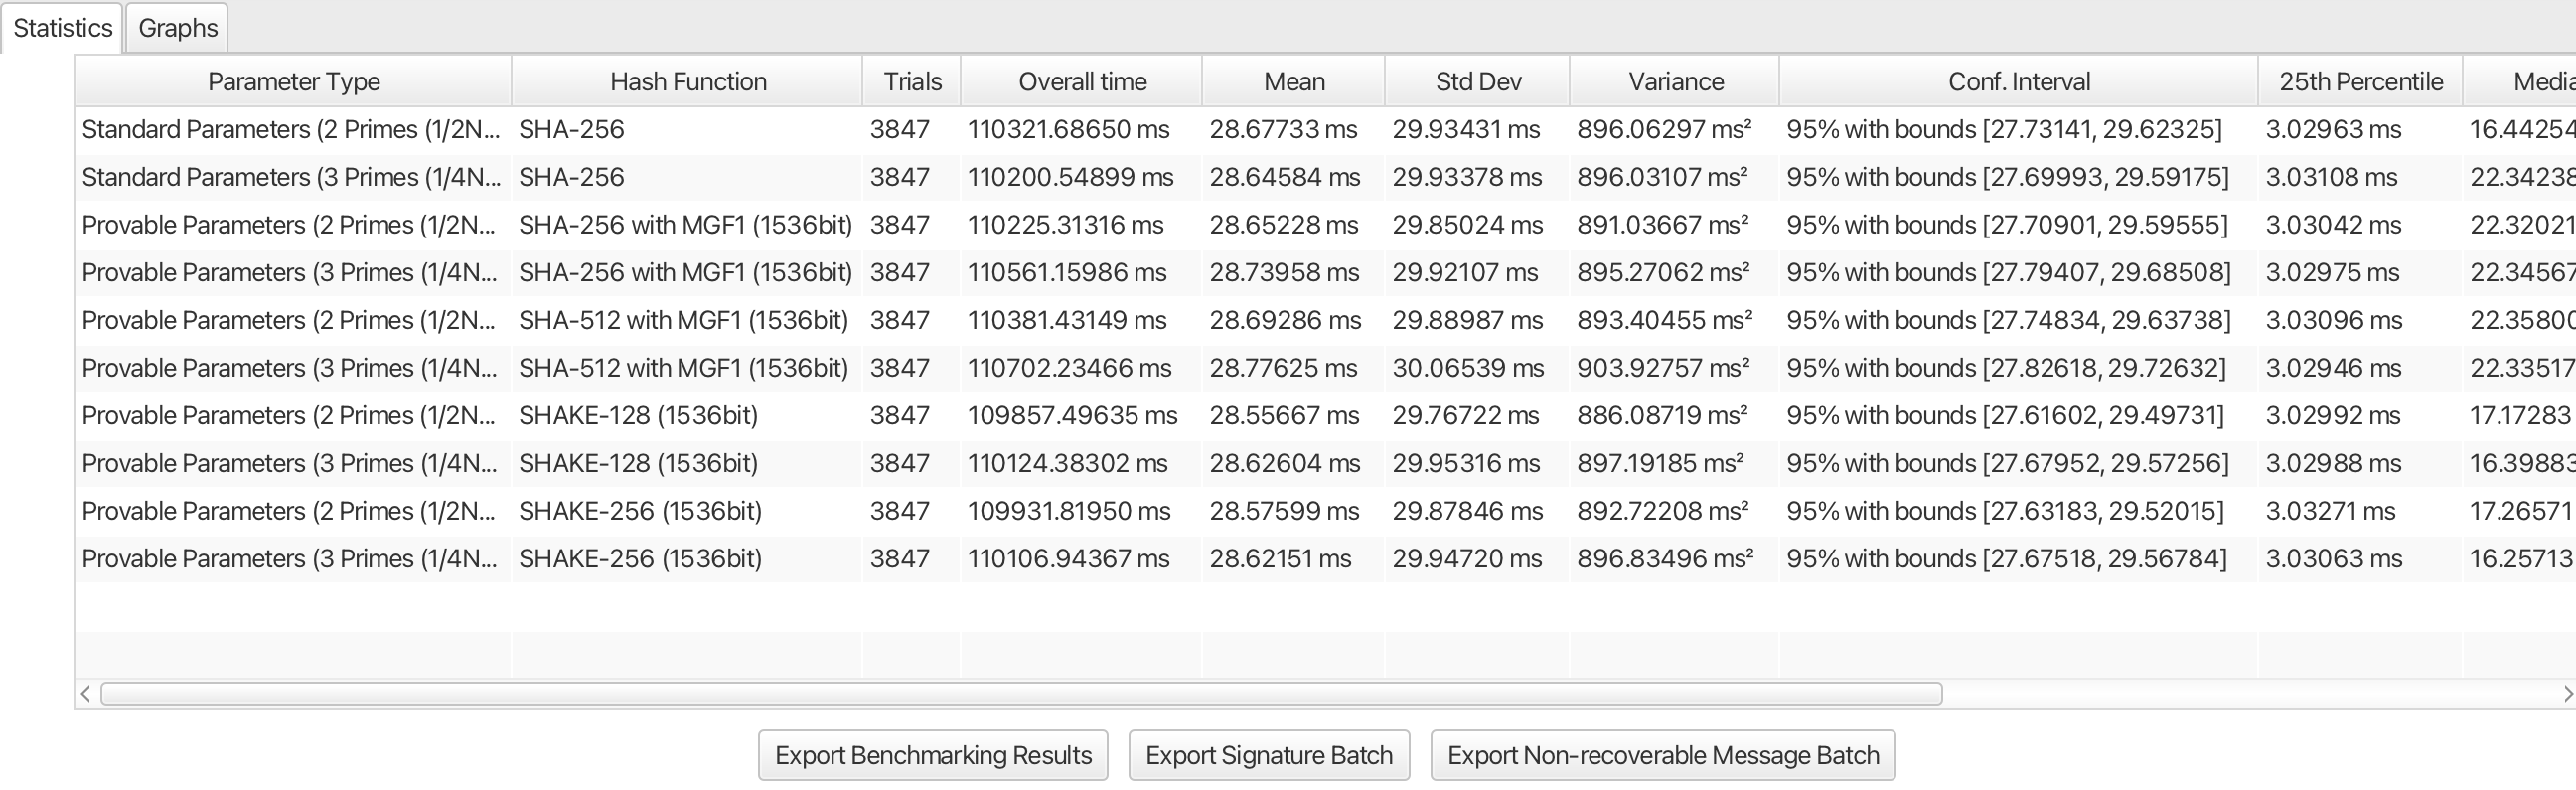
\includegraphics[width=\textwidth]{main_pictures/iso/iso_sign_3072bit_table1_1.png}} 
        \fbox{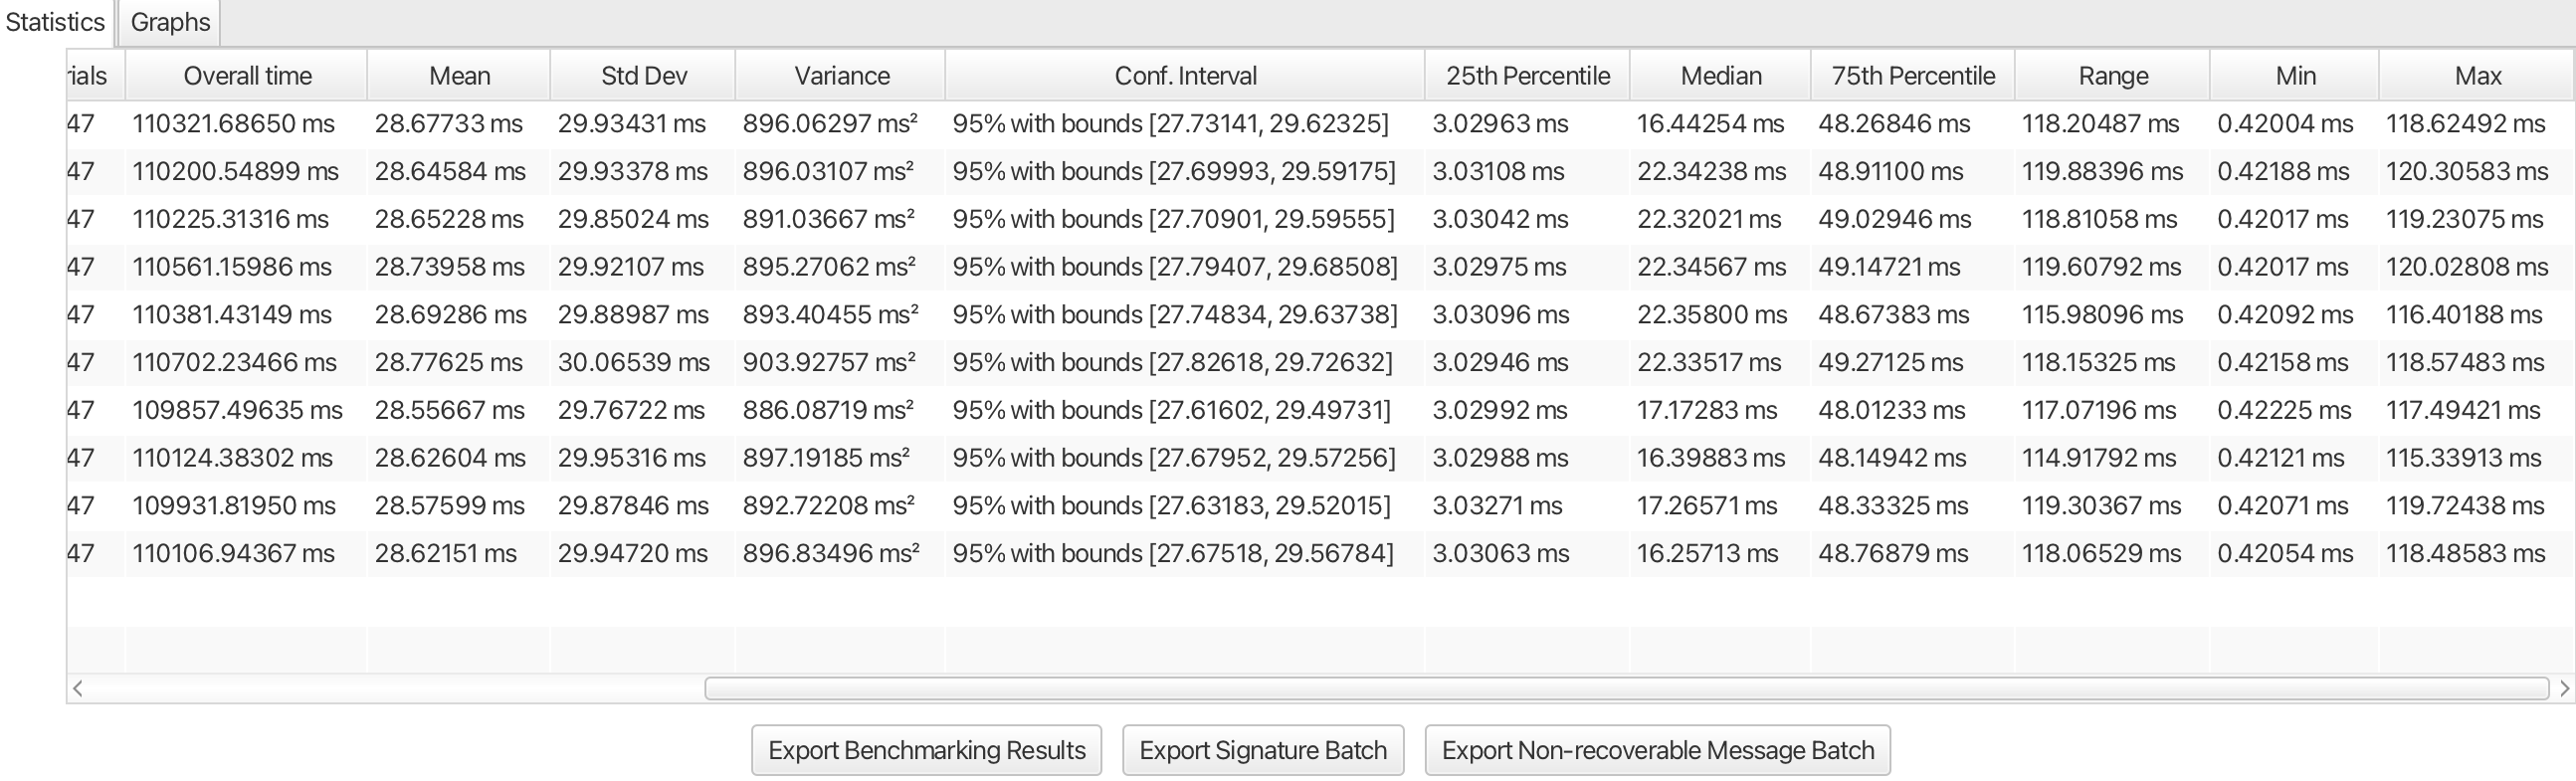
\includegraphics[width=\textwidth]{main_pictures/iso/iso_sign_3072bit_table2_1.png}}
    \end{minipage}
         \label{iso_sign_3072bit_table}
\end{figure}

\begin{figure}[H]
    \centering % Center the images
     \caption{Instantiation of ISO/IEC 9796-2:2010 Signature Scheme 1 with standard vs provably secure parameters (4096-bit Key Size) for signature creation}
    % First image in a minipage
    \begin{minipage}{\textwidth}
        \centering
        \fbox{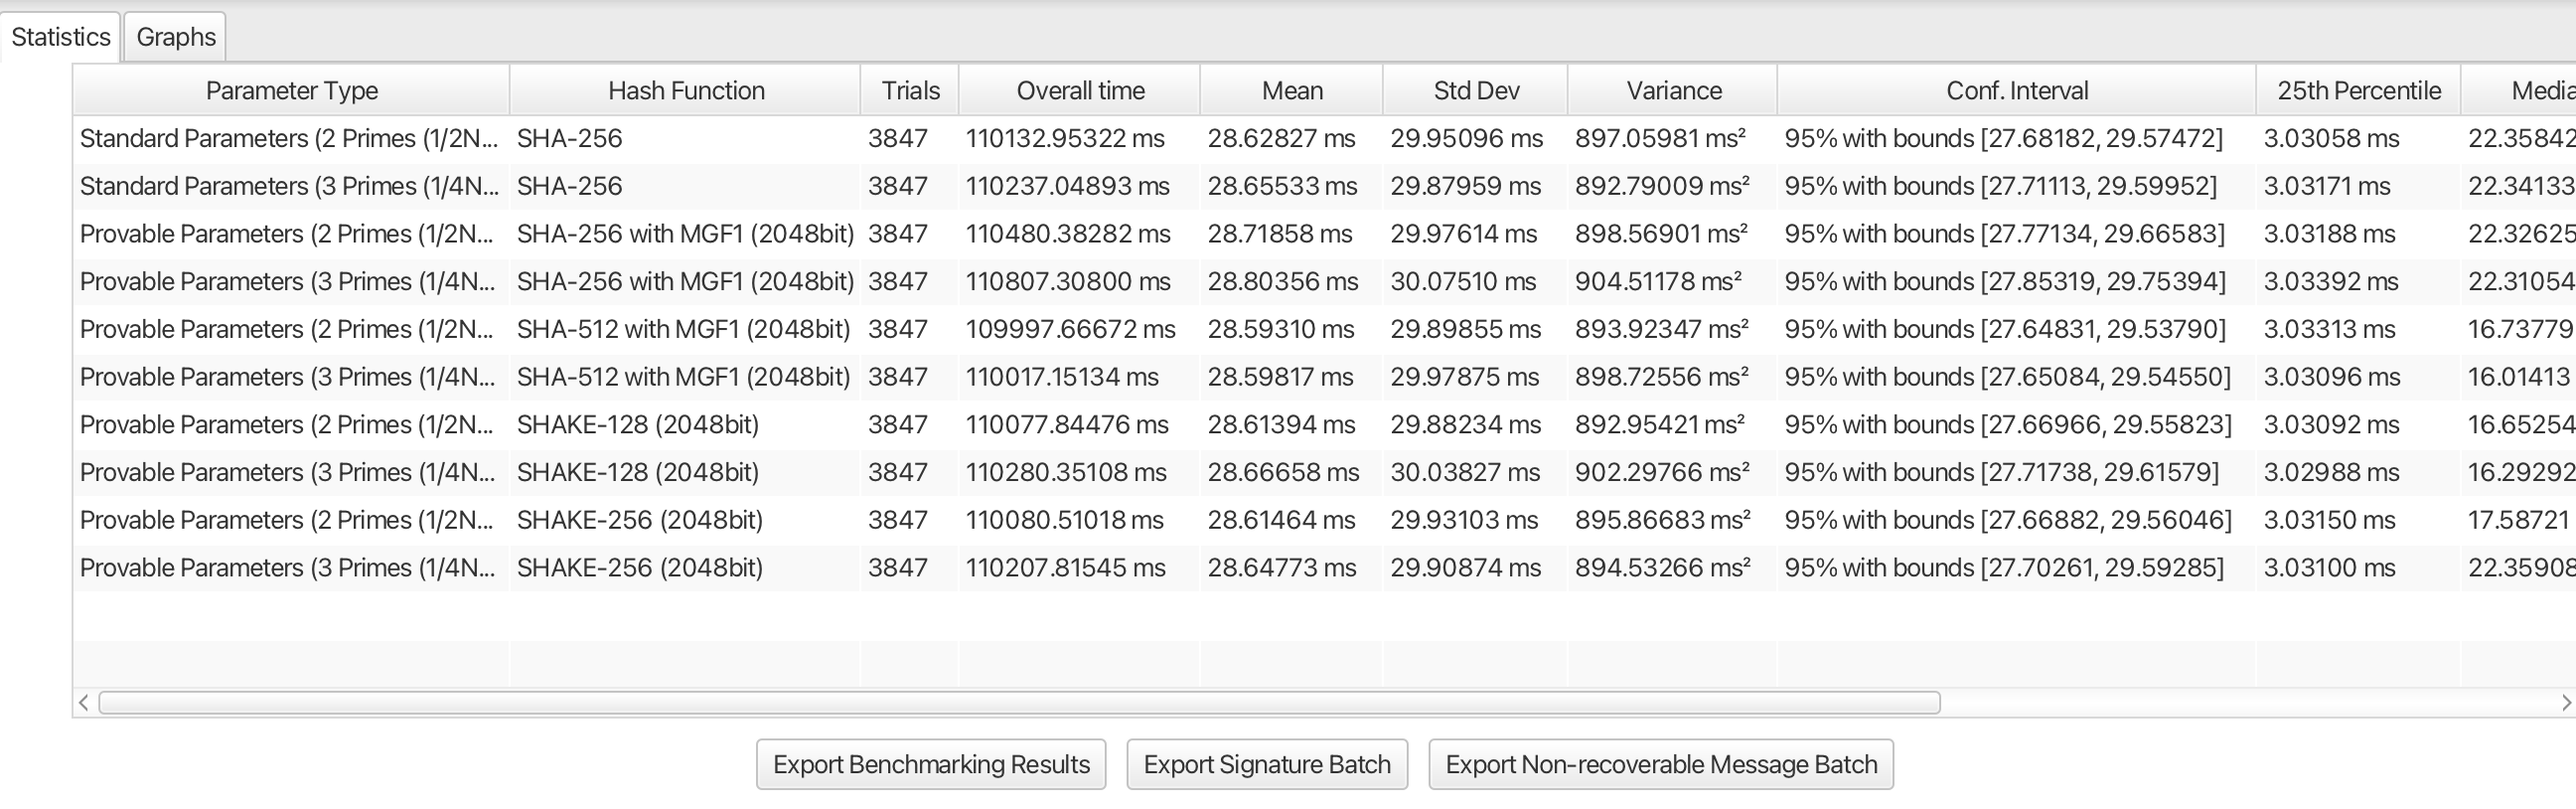
\includegraphics[width=\textwidth]{main_pictures/iso/iso_sign_4096bit_table1_1.png}} 
        \fbox{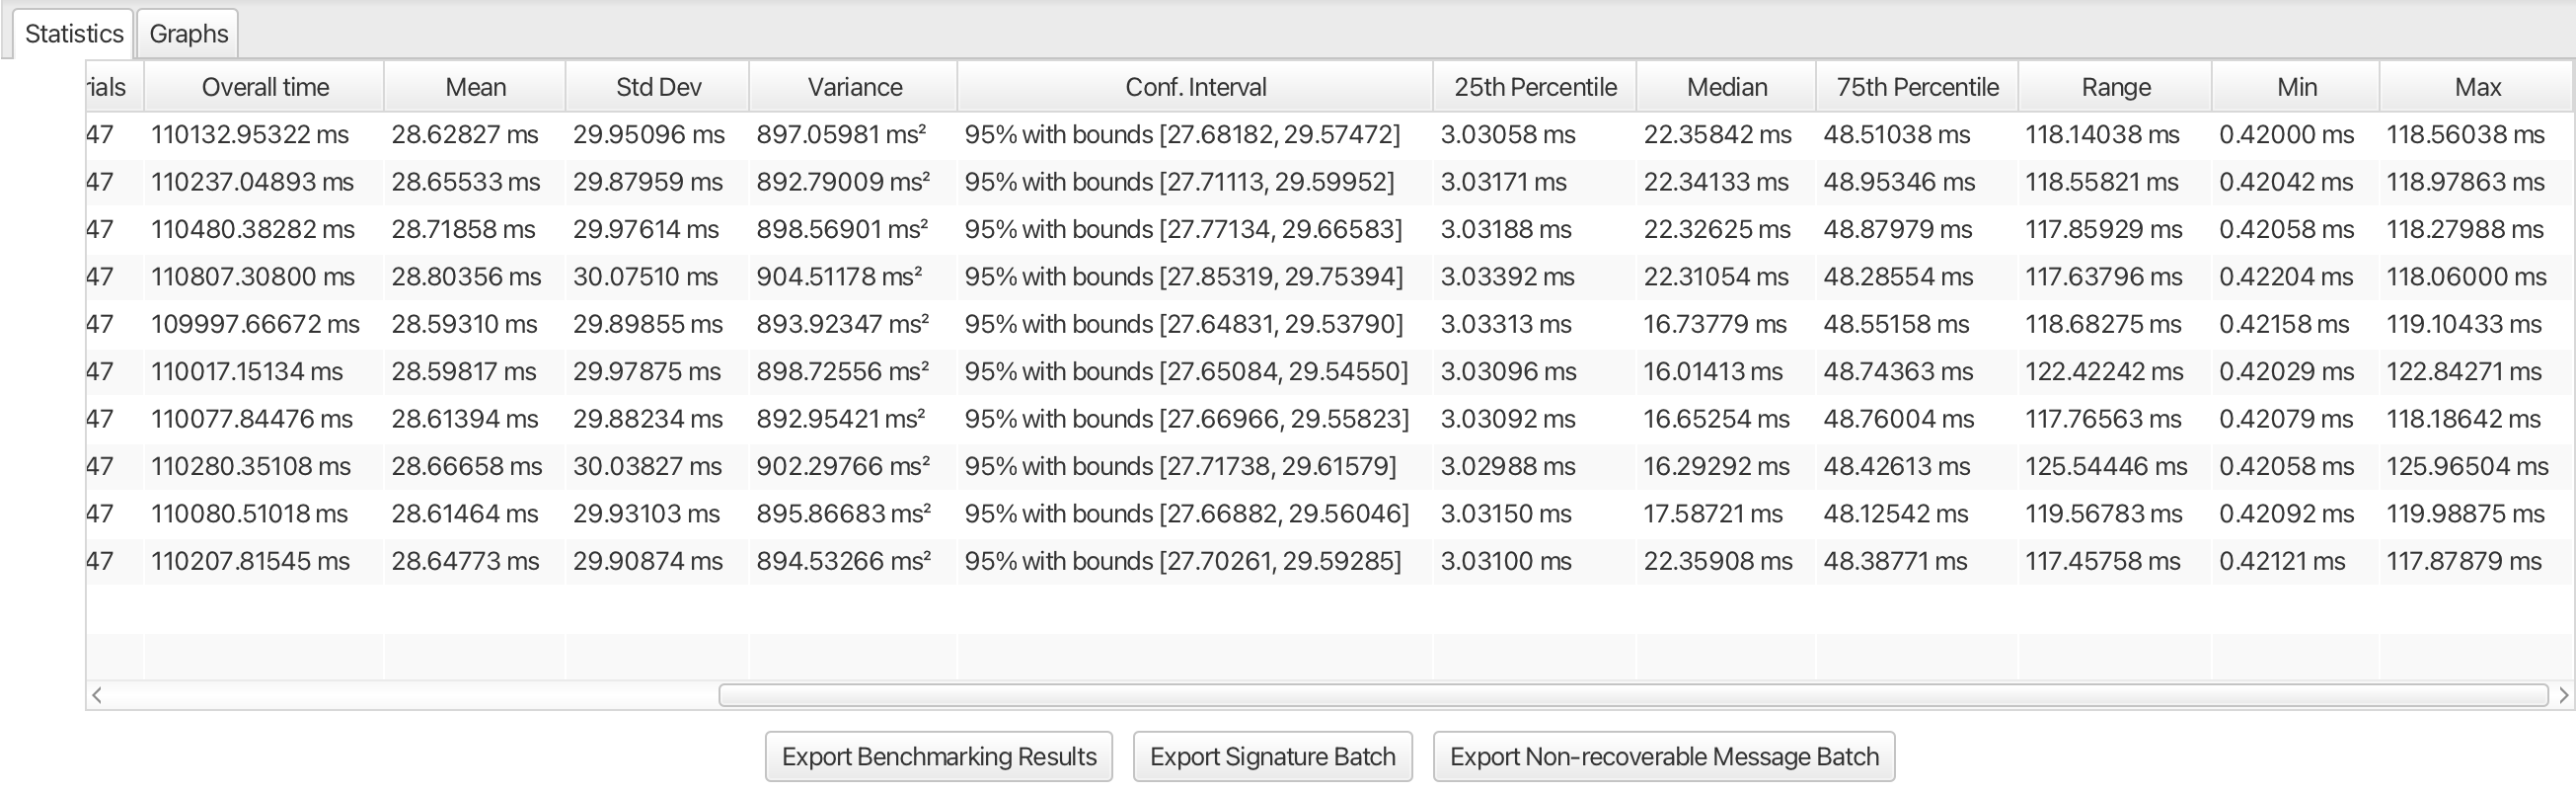
\includegraphics[width=\textwidth]{main_pictures/iso/iso_sign_4096bit_table2_1.png}}
    \end{minipage}
             \label{iso_sign_4096bit_table}
\end{figure}

\begin{figure}[H]
    \centering % Center the images
     \caption{Instantiation of ISO/IEC 9796-2:2010 Signature Scheme 1 with standard vs provably secure parameters (5120-bit Key Size) for signature creation}
    % First image in a minipage
    \begin{minipage}{\textwidth}
        \centering
        \fbox{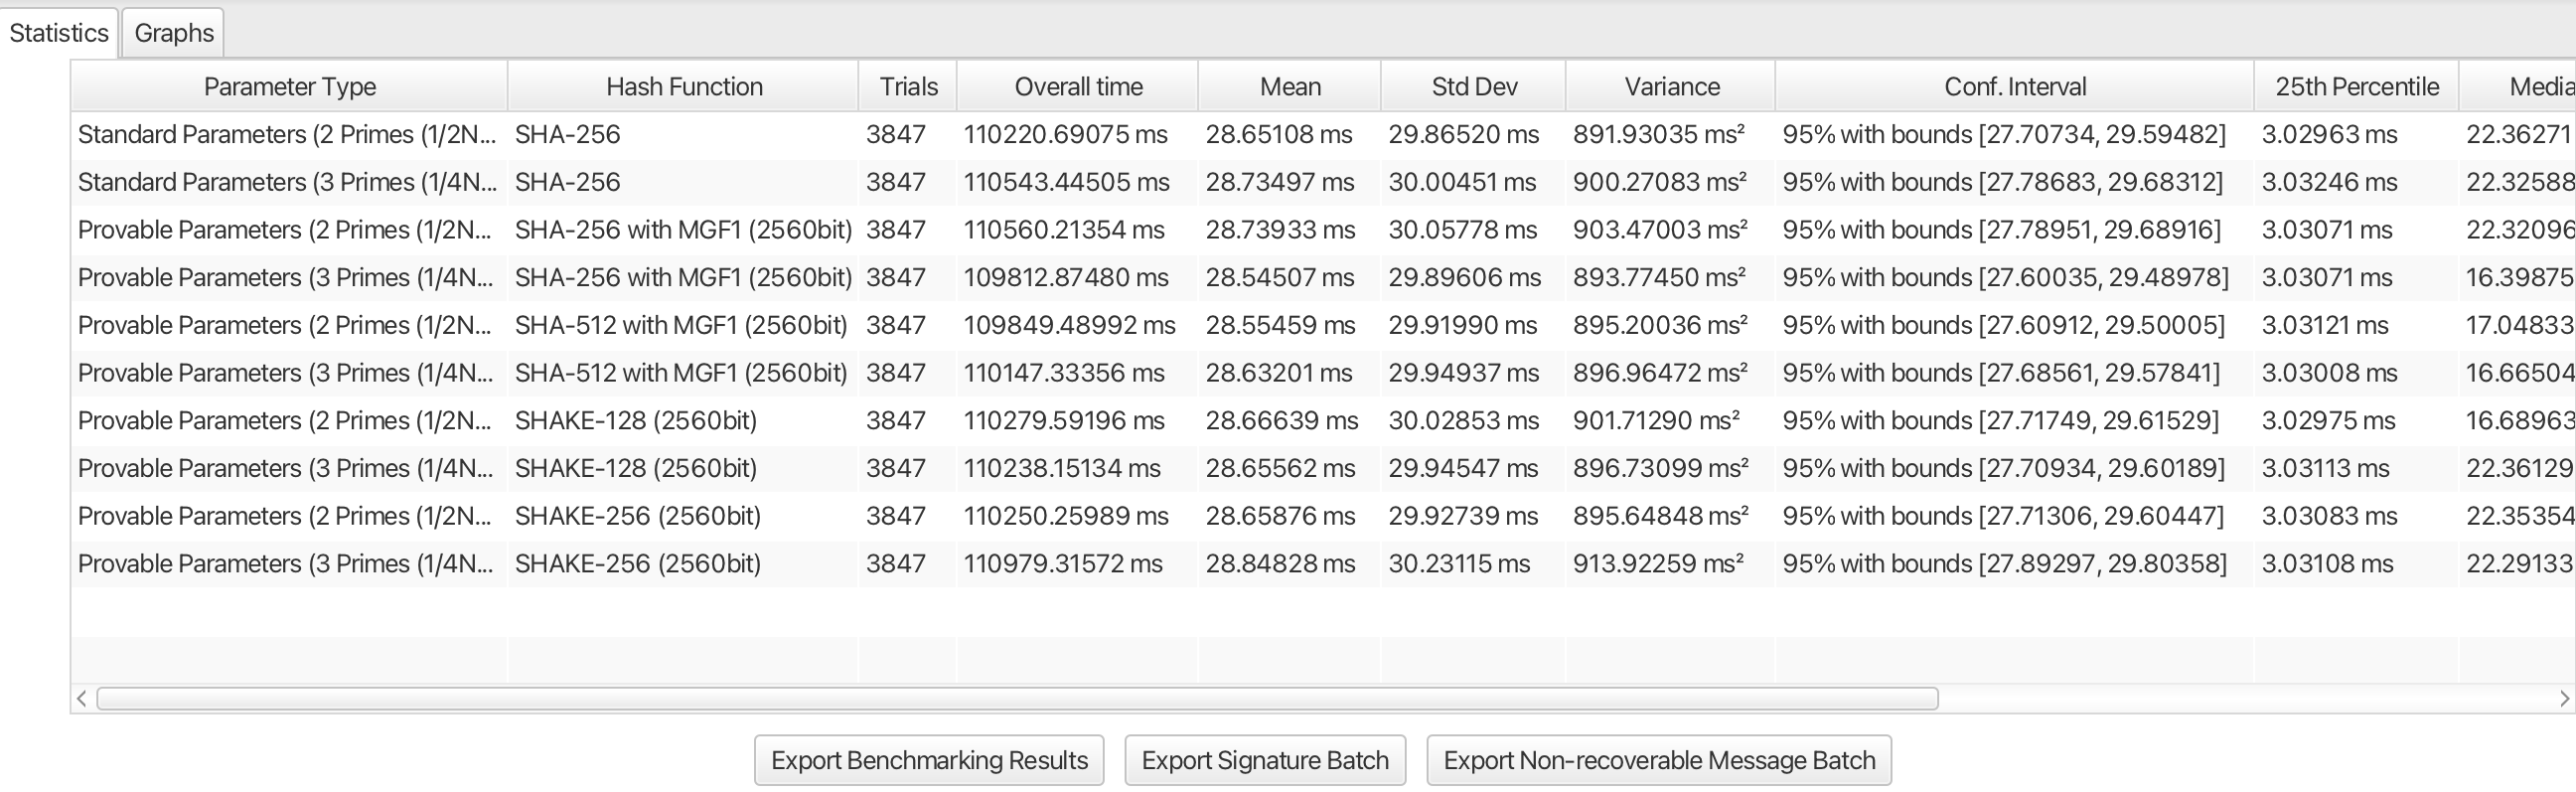
\includegraphics[width=\textwidth]{main_pictures/iso/iso_sign_5120bit_table1_1.png}} 
        \fbox{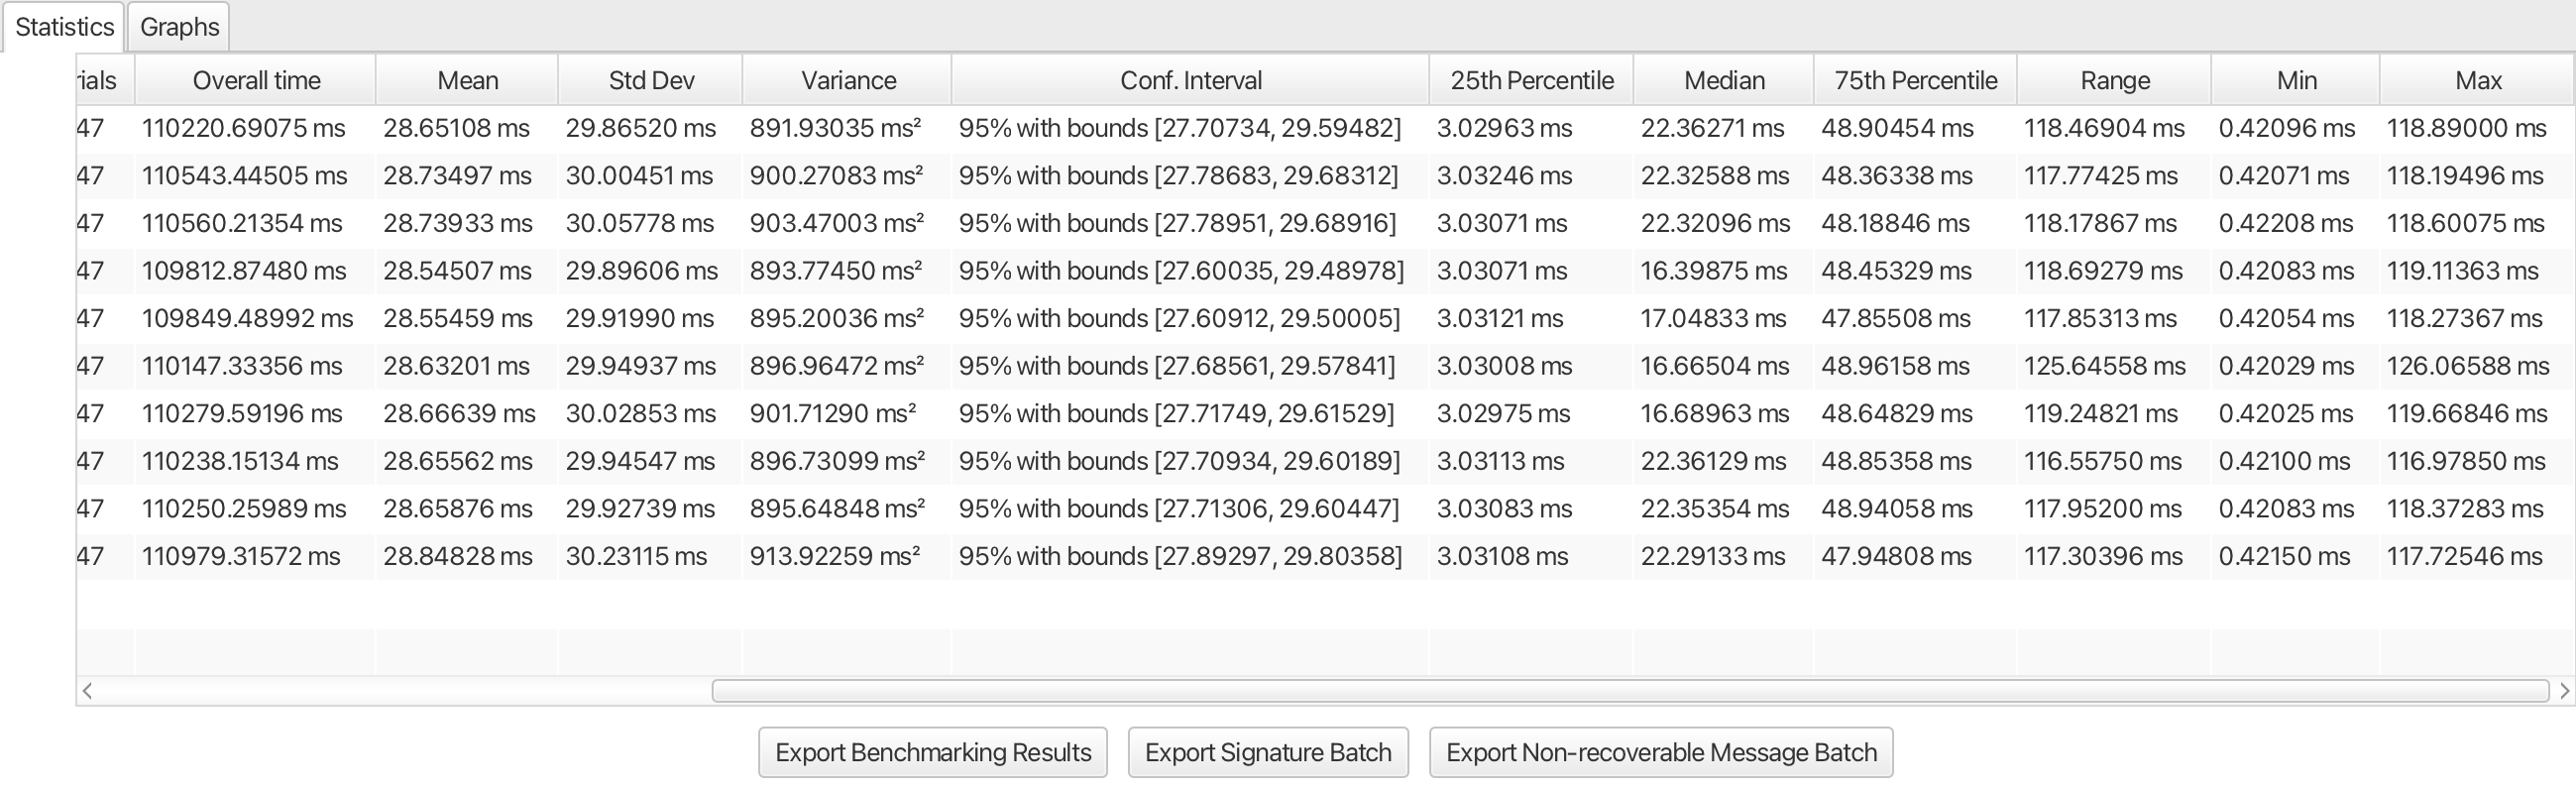
\includegraphics[width=\textwidth]{main_pictures/iso/iso_sign_5120bit_table2_1.png}}
    \end{minipage}
     \label{iso_sign_5120bit_table}
\end{figure}

\begin{figure}[H]
    \centering % Center the images
     \caption{Instantiation of ISO/IEC 9796-2:2010 Signature Scheme 1 with standard vs provably secure parameters (6144-bit Key Size) for signature creation}
    % First image in a minipage
    \begin{minipage}{\textwidth}
        \centering
        \fbox{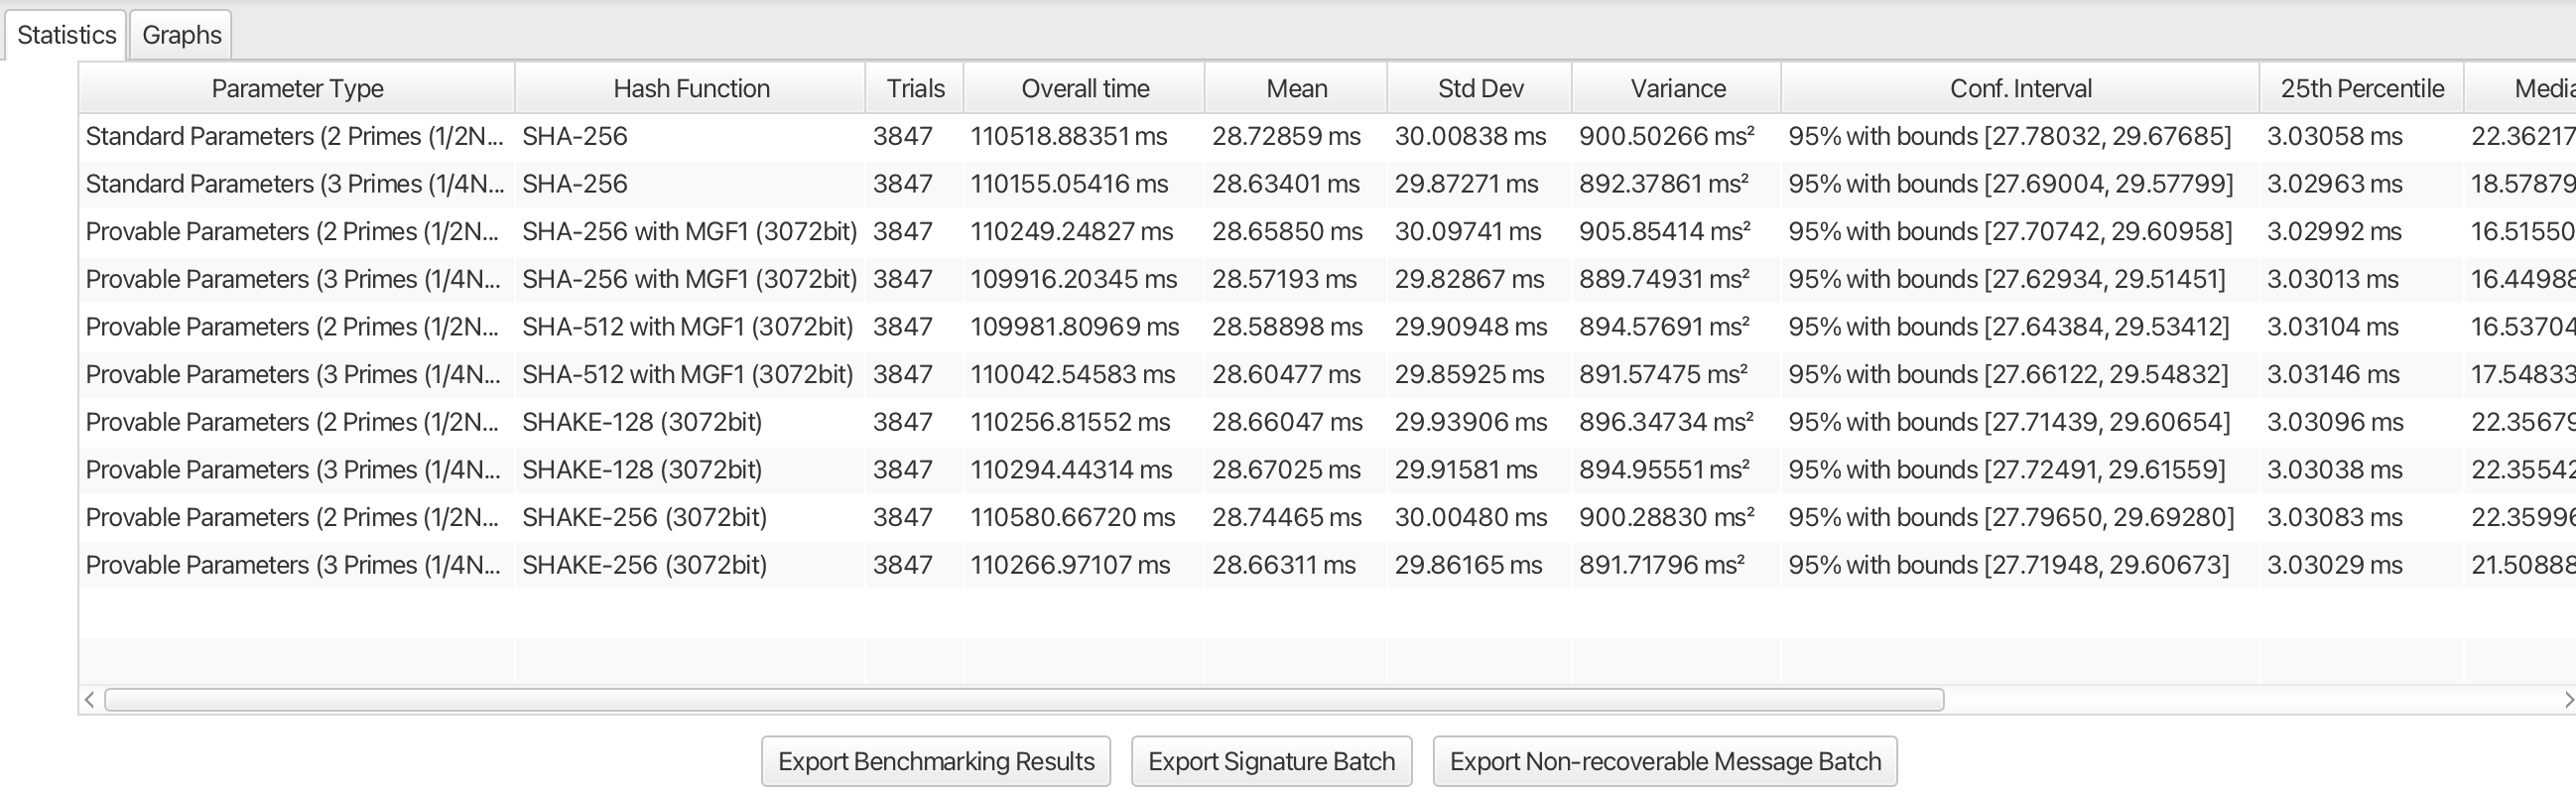
\includegraphics[width=\textwidth]{main_pictures/iso/iso_sign_6144bit_table1_1.png}} 
        \fbox{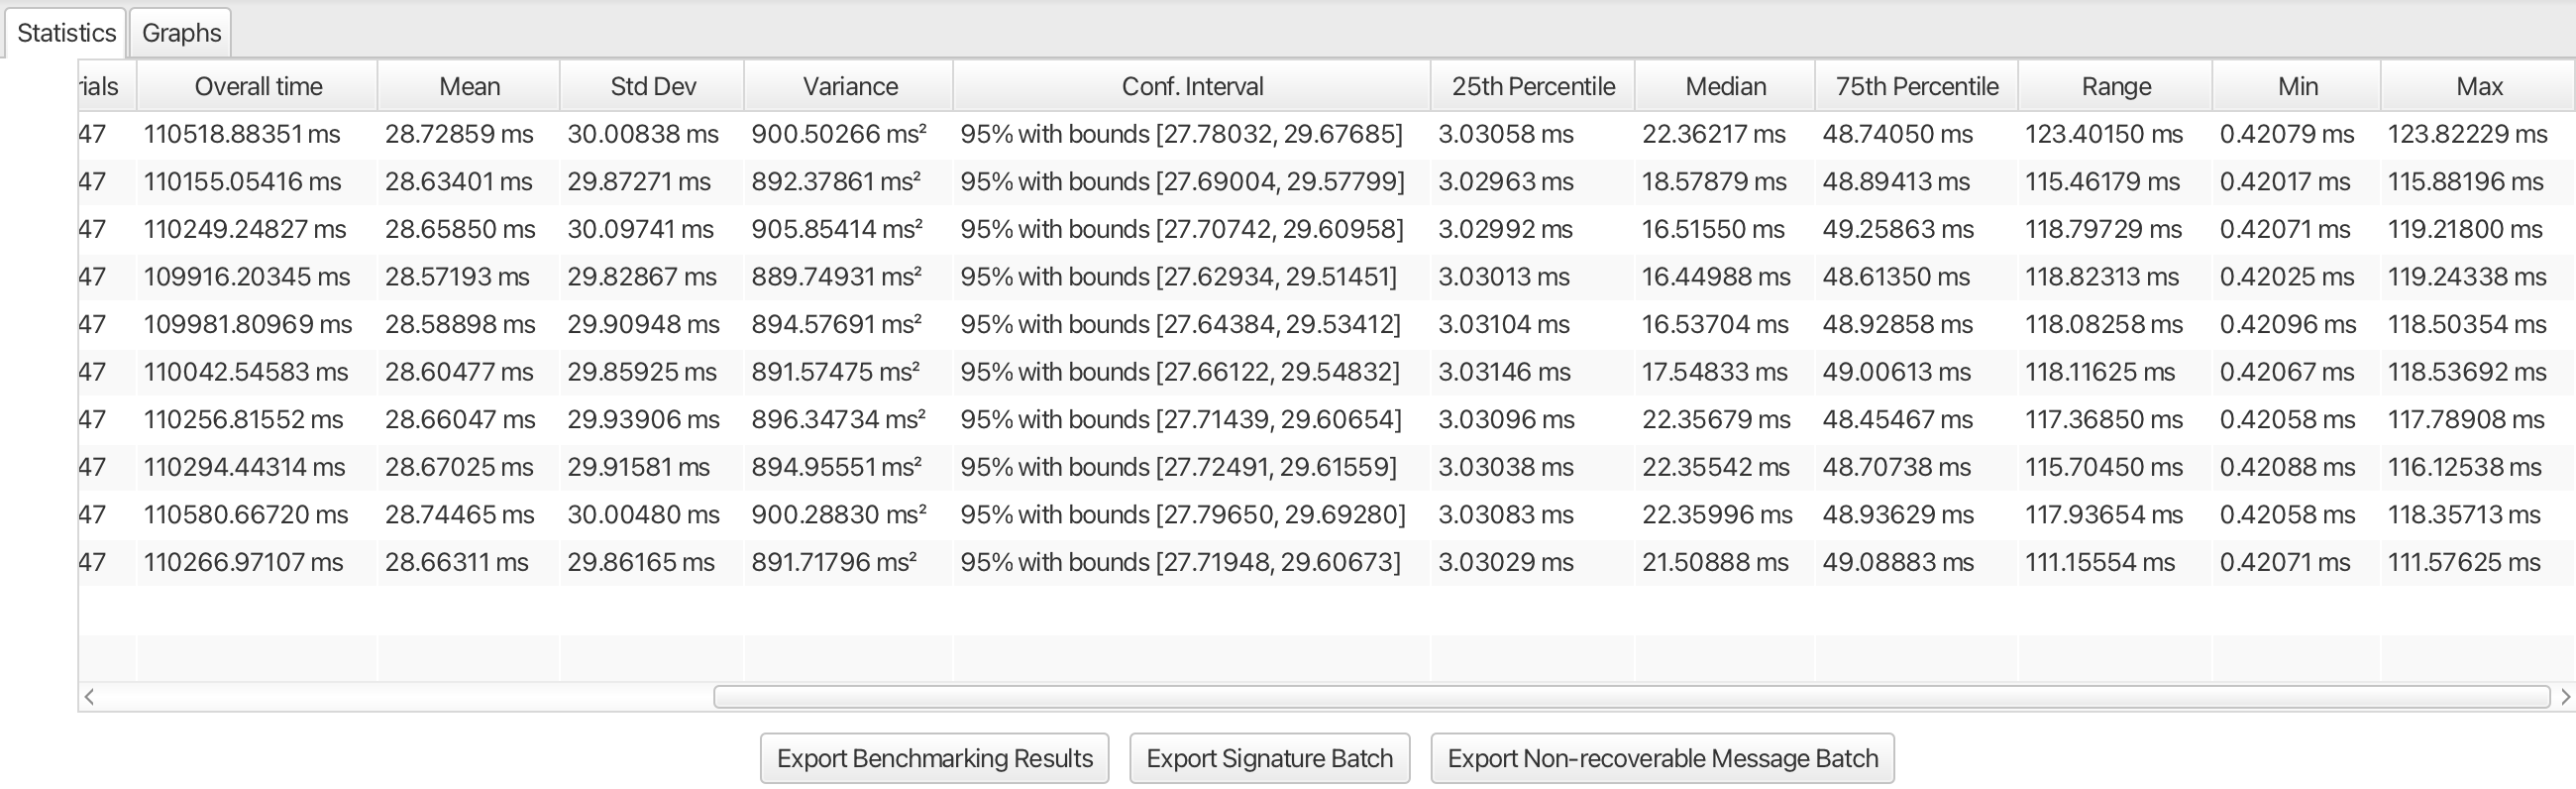
\includegraphics[width=\textwidth]{main_pictures/iso/iso_sign_6144bit_table2_1.png}}
    \end{minipage}
         \label{iso_sign_6144bit_table}
\end{figure}

The ISO/IEC 9796-2:2010 Signature Scheme 1 exhibits a similar performance profile in its benchmarking for signature creation across all key sizes. Standard parameters using two primes for SHA-256 show mean times between 28.57240 ms and 28.72859 ms. For provably secure parameters with two primes, the mean times across different hash functions vary from 28.48672 ms to 28.74465 ms, demonstrating a performance variation of up to 1.39\%. With three primes, standard parameters yield mean times from 28.60973 ms to 28.73497 ms, while for provably secure parameters, the range is from 28.54507 ms to 28.80356 ms, indicating a potential variation of up to 1.49\% across all key sizes.


Like the former two schemes ISO/IEC 9796-2:2010 Signature Scheme 1 demonstrates that the use of provably secure parameters for signature creation yields only negligible differences in performance when compared to standard parameters.  The small fluctuations in performance times are likely inherent to computational processes and do not signify any significant statistical difference. Therefore it can be inferred that instantiation of ISO-IEC 9796-2 Scheme 1 (for signature creation) with provably secure parameters does not introduce an overhead, and rather maintains effectiveness in line with standard parameters.



\begin{comment}
Overall, the benchmarking results for ISO-IEC 9796-2 Scheme 1 signature creation also exhibit minor differences between standard and provably secure parameters. These small fluctuations in performance times across different key sizes and configurations can likely be ascribed to inherent variations in computational processes rather than distinct impacts of the parameter choices. The standard deviations and confidence intervals provide further evidence that these variations are tightly grouped, suggesting a lack of significant statistical difference. Therefore, similar to the PKCS\#1 v1.5 and ANSI X9.31 rDSA  results, it can be inferred that using provably secure parameters in ISO-IEC 9796-2 Scheme 1 does not introduce an overhead, and rather maintains effectiveness in line with standard parameters.
\end{comment}




\section{Signature Verification Results (ANSI X9.31 rDSA)}

\begin{figure}[H]
    \centering % Center the images
     \caption{Instantiation of ANSI X9.31 rDSA with standard vs provably secure parameters (1024-bit Key Size) for signature verification}
    % First image in a minipage
    \begin{minipage}{\textwidth}
        \centering
        \fbox{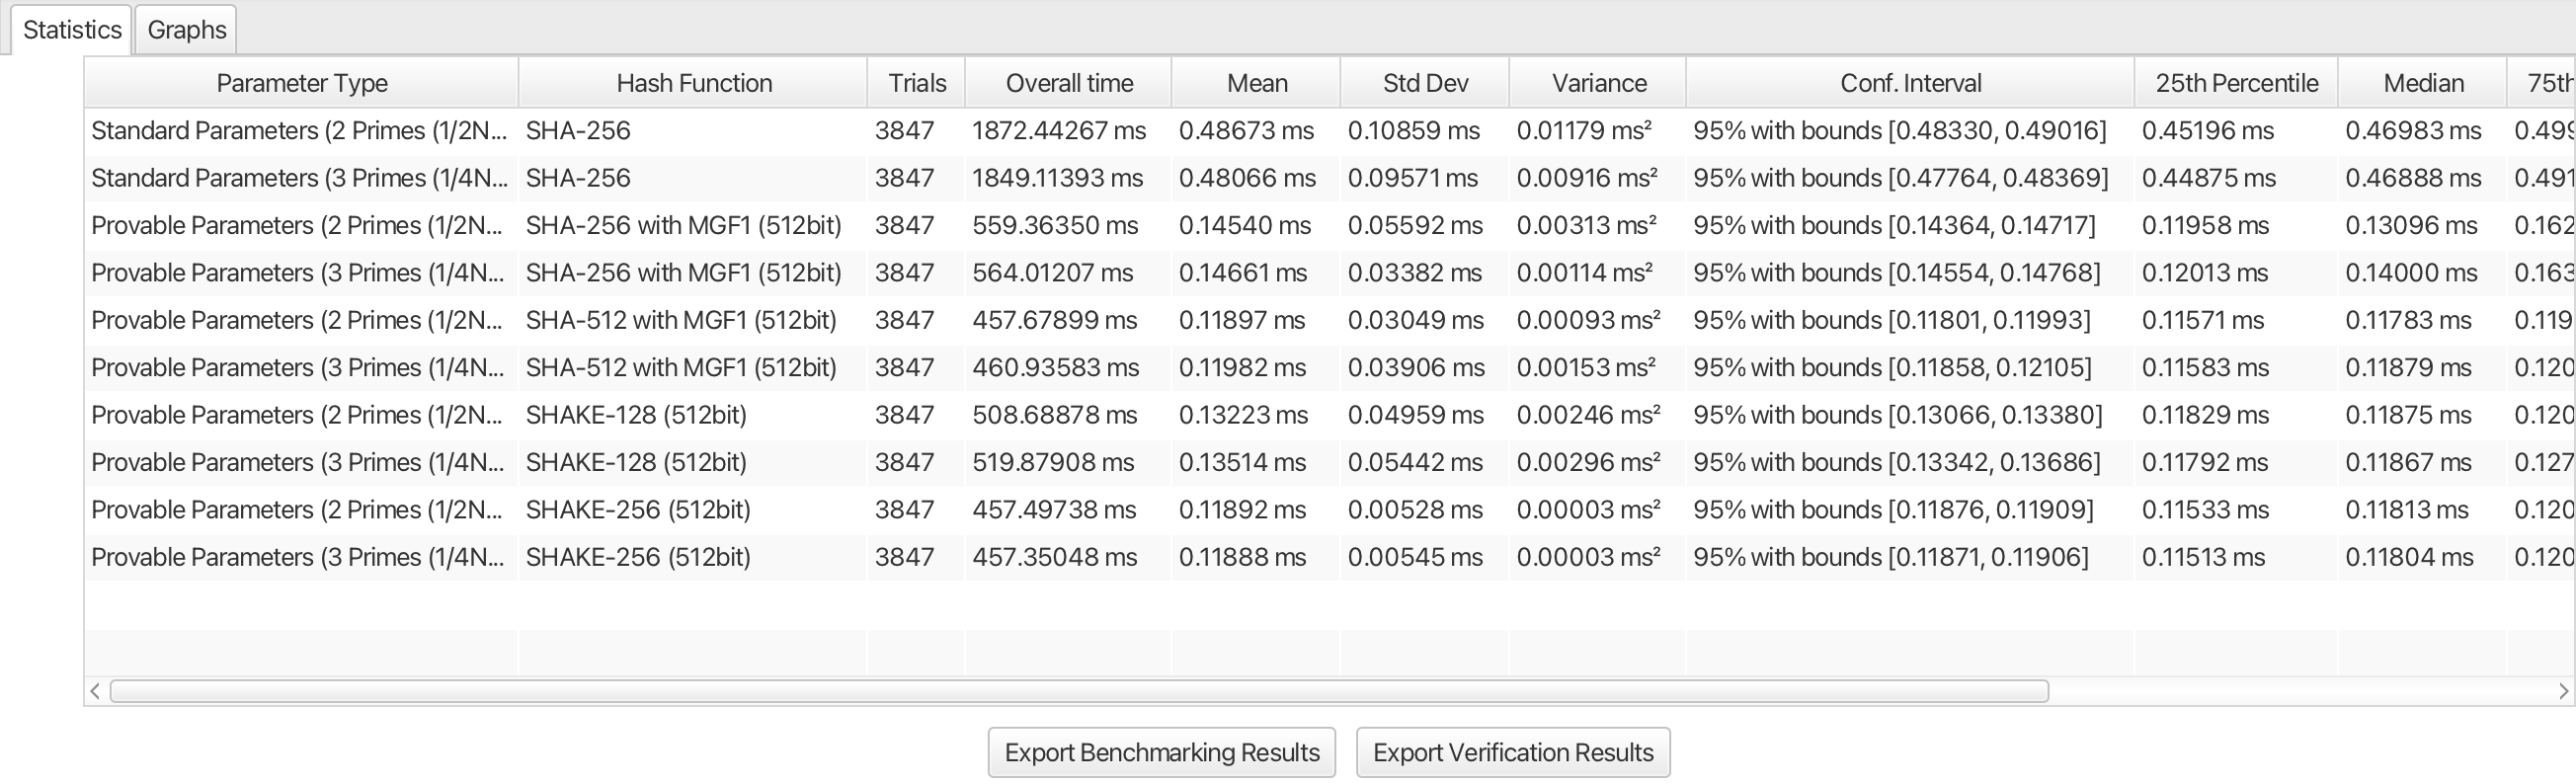
\includegraphics[width=\textwidth]{main_pictures/ansi/ansi_verify_1024bit_table1_1.png}} 
        \fbox{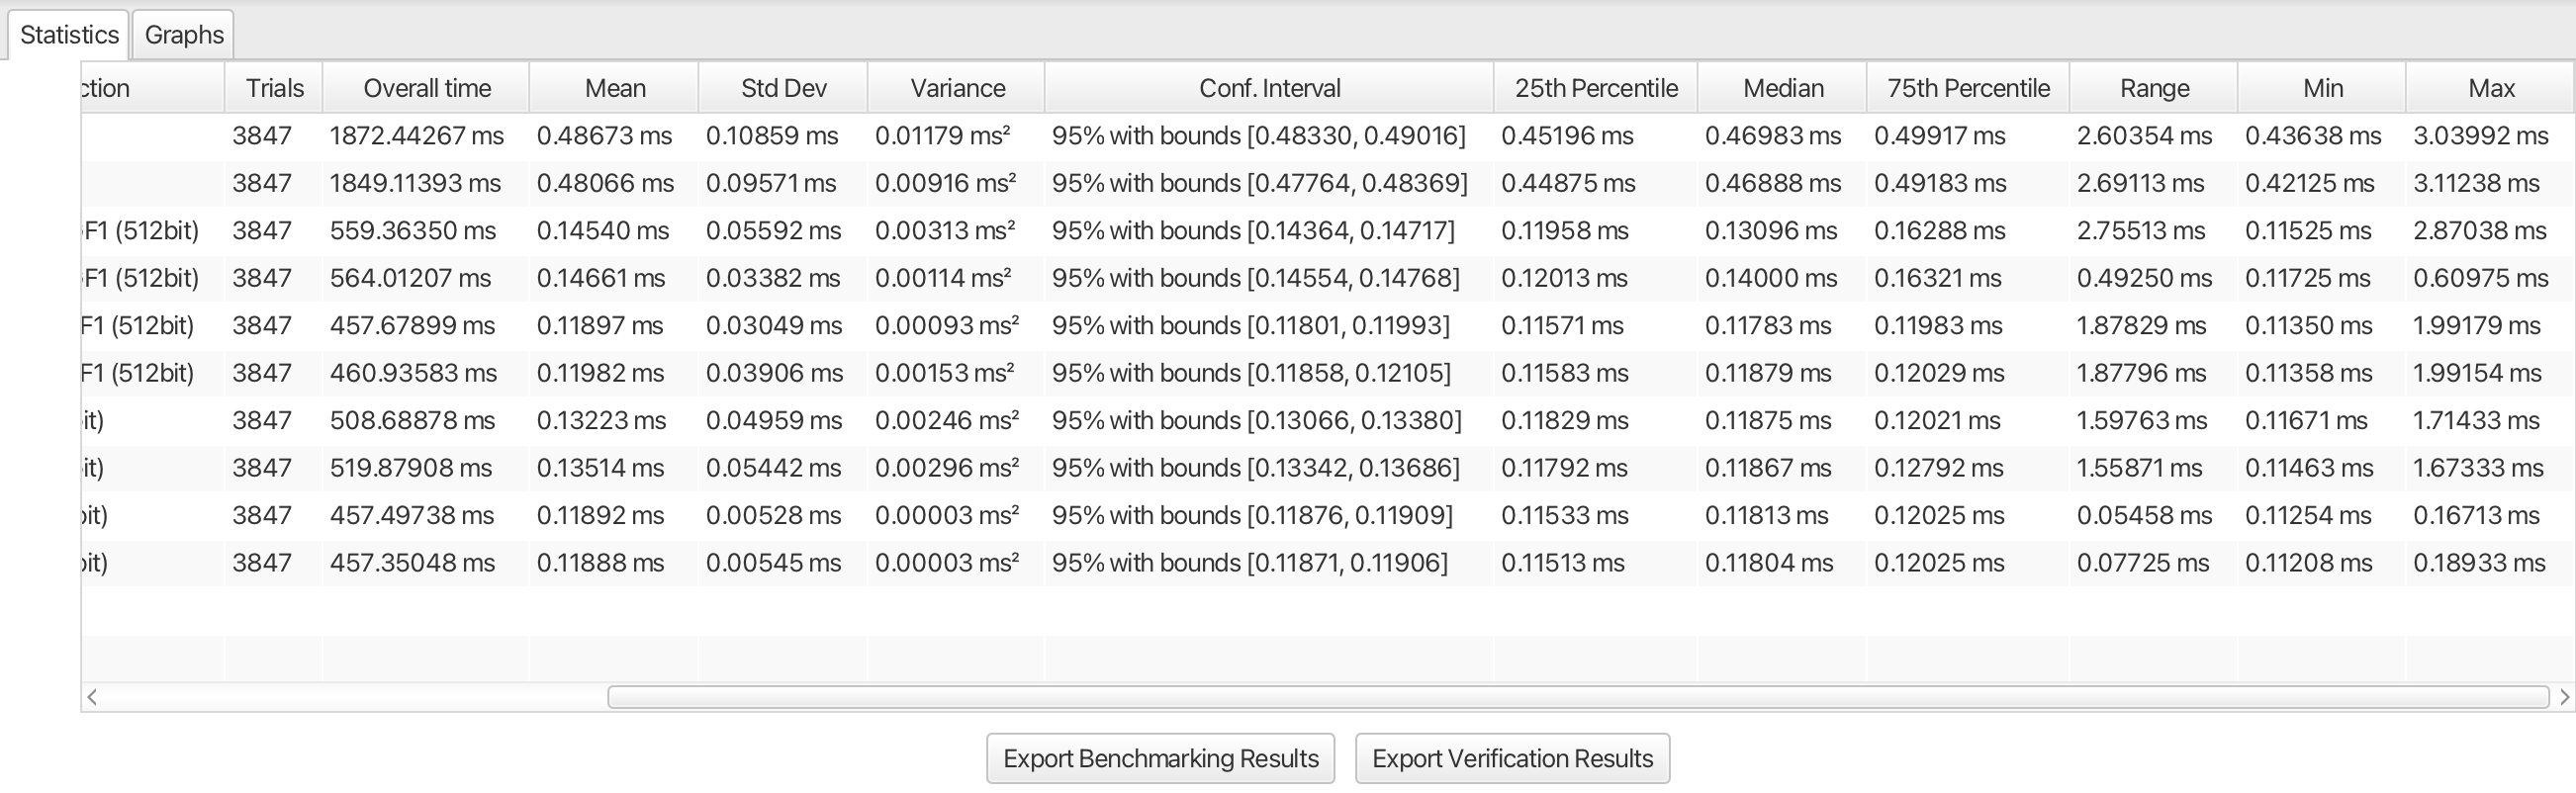
\includegraphics[width=\textwidth]{main_pictures/ansi/ansi_verify_1024bit_table2_1.png}}
    \end{minipage}
       \label{ansi_verify_1024bit_table}
  \end{figure}
  
\begin{figure}[H]
    \centering % Center the images
     \caption{Instantiation of ANSI X9.31 rDSA with standard vs provably secure parameters (2048-bit Key Size) for signature verification}
    % First image in a minipage
    \begin{minipage}{\textwidth}
        \centering
        \fbox{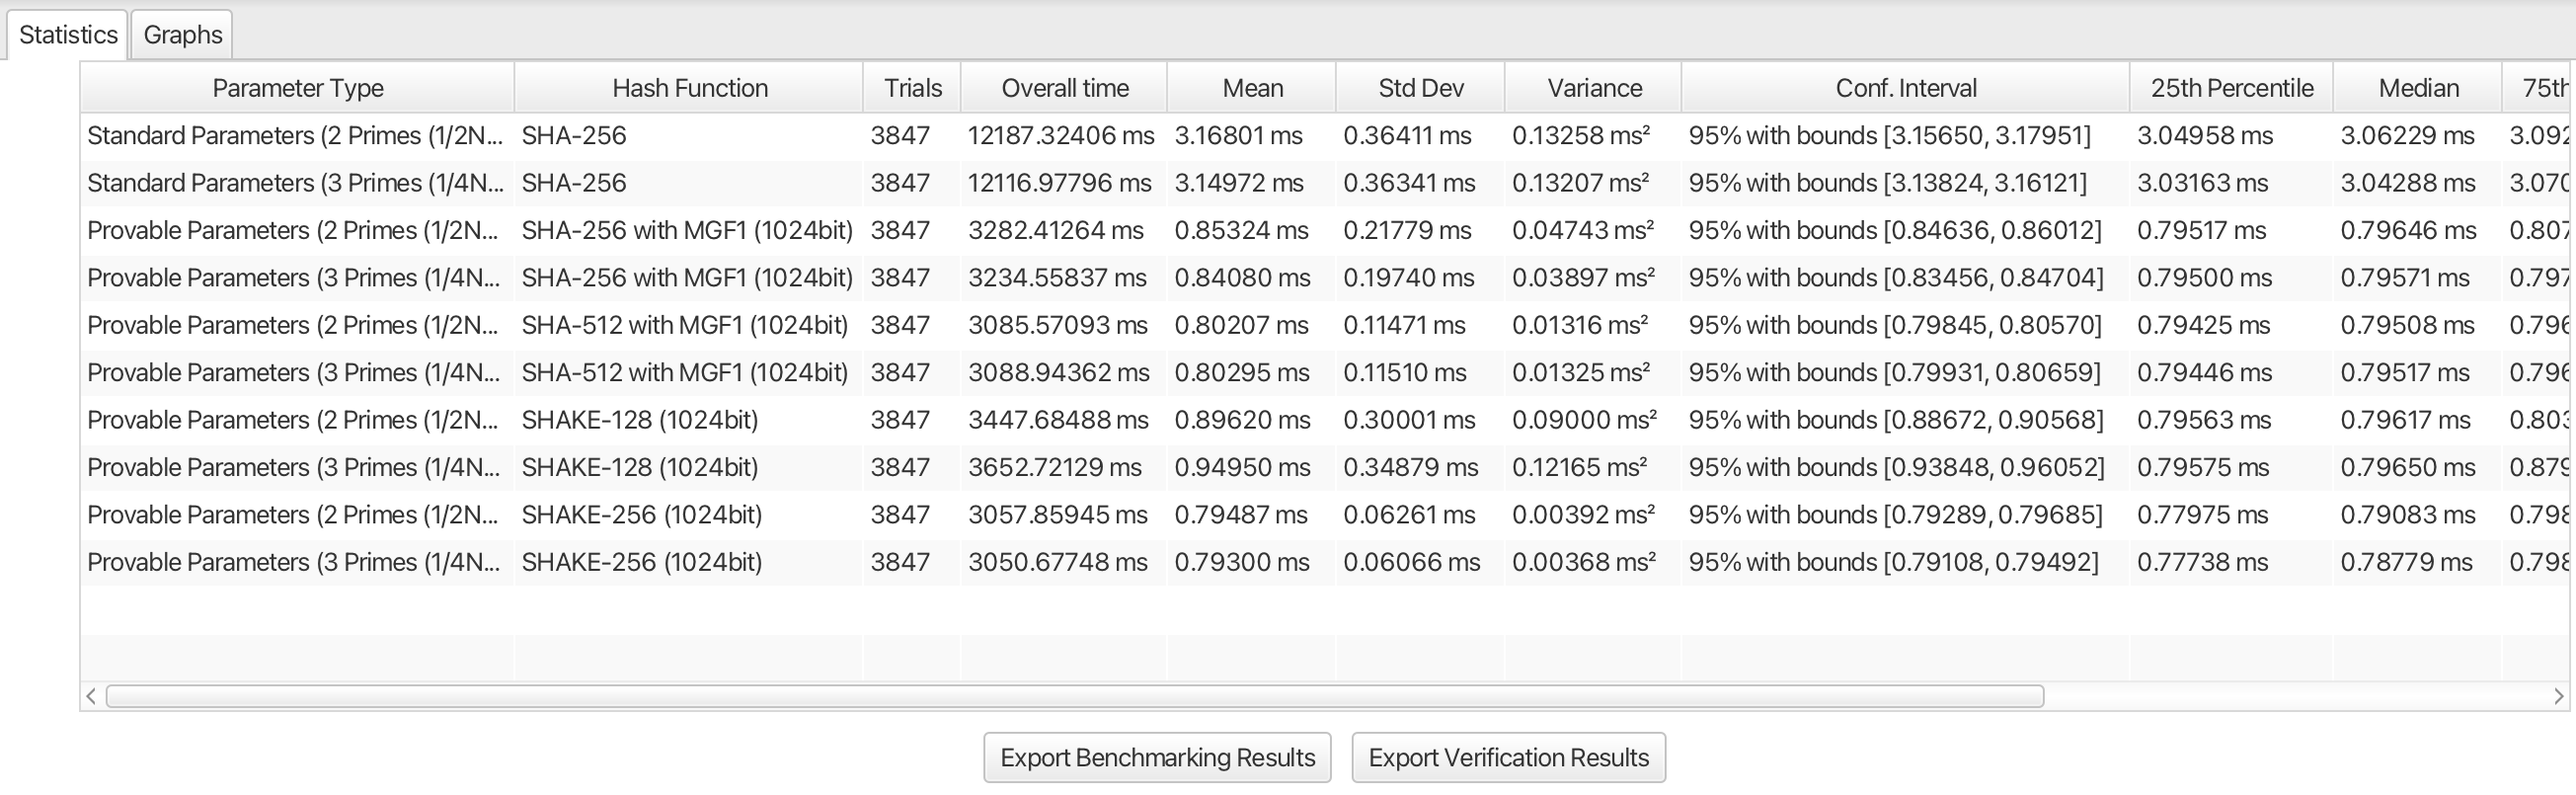
\includegraphics[width=\textwidth]{main_pictures/ansi/ansi_verify_2048bit_table1_1.png}} 
        \fbox{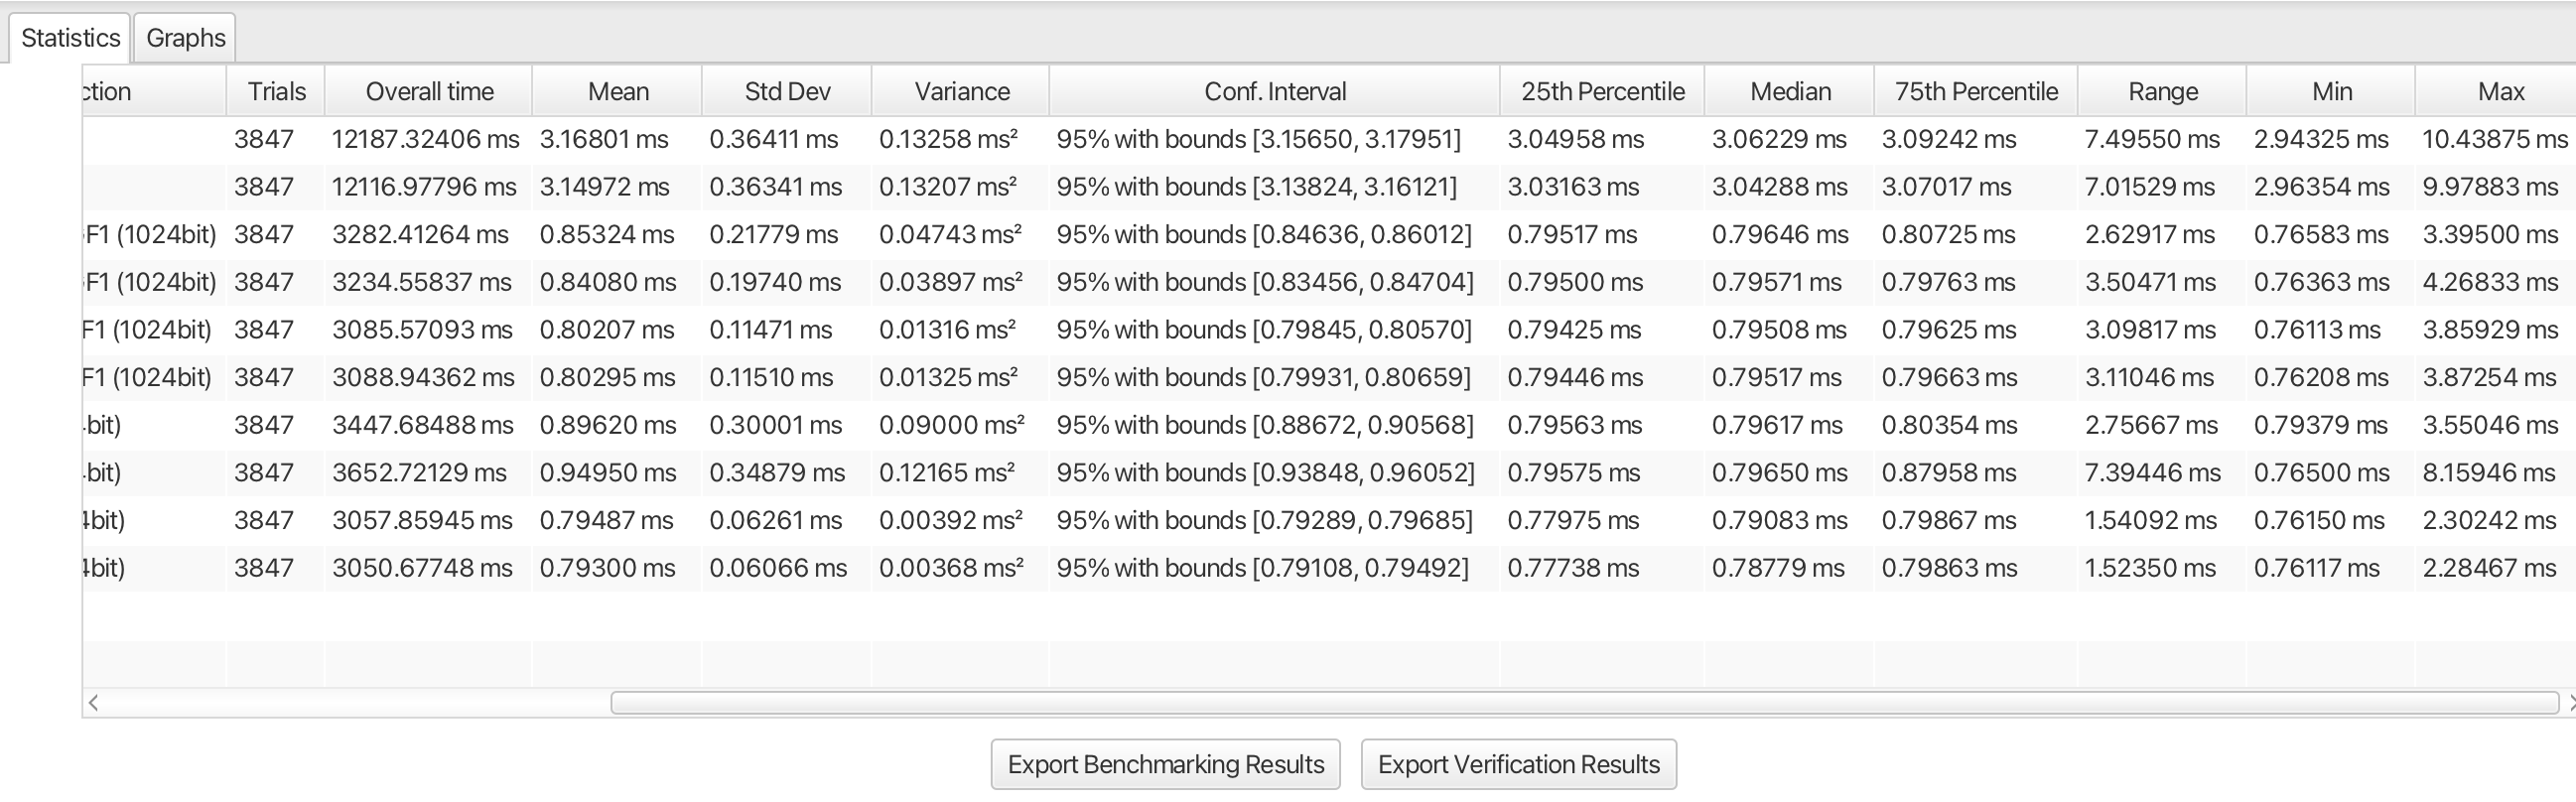
\includegraphics[width=\textwidth]{main_pictures/ansi/ansi_verify_2048bit_table2_1.png}}
    \end{minipage}
           \label{ansi_verify_2048bit_table}
  \end{figure}
  
\begin{figure}[H]
    \centering % Center the images
     \caption{Instantiation of ANSI X9.31 rDSA with standard vs provably secure parameters (3072-bit Key Size) for signature verification}
    % First image in a minipage
    \begin{minipage}{\textwidth}
        \centering
        \fbox{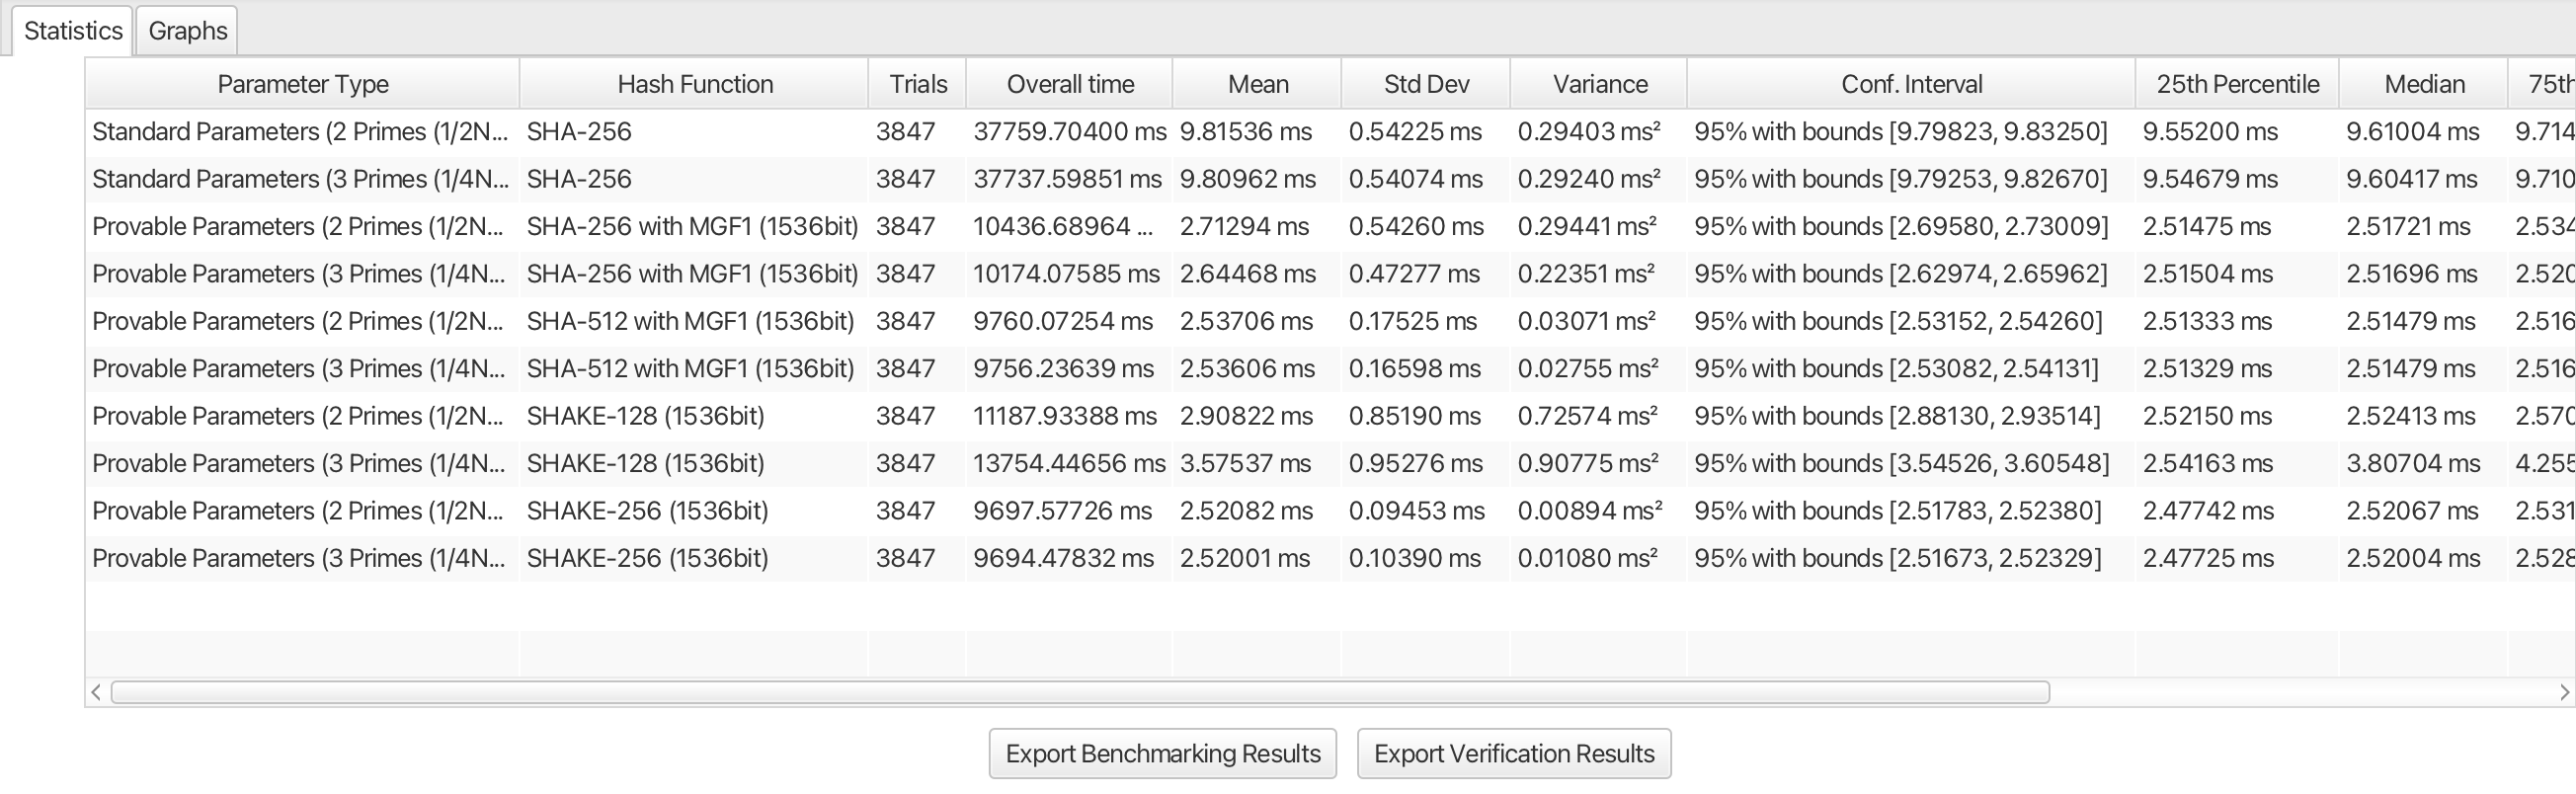
\includegraphics[width=\textwidth]{main_pictures/ansi/ansi_verify_3072bit_table1_1.png}} 
        \fbox{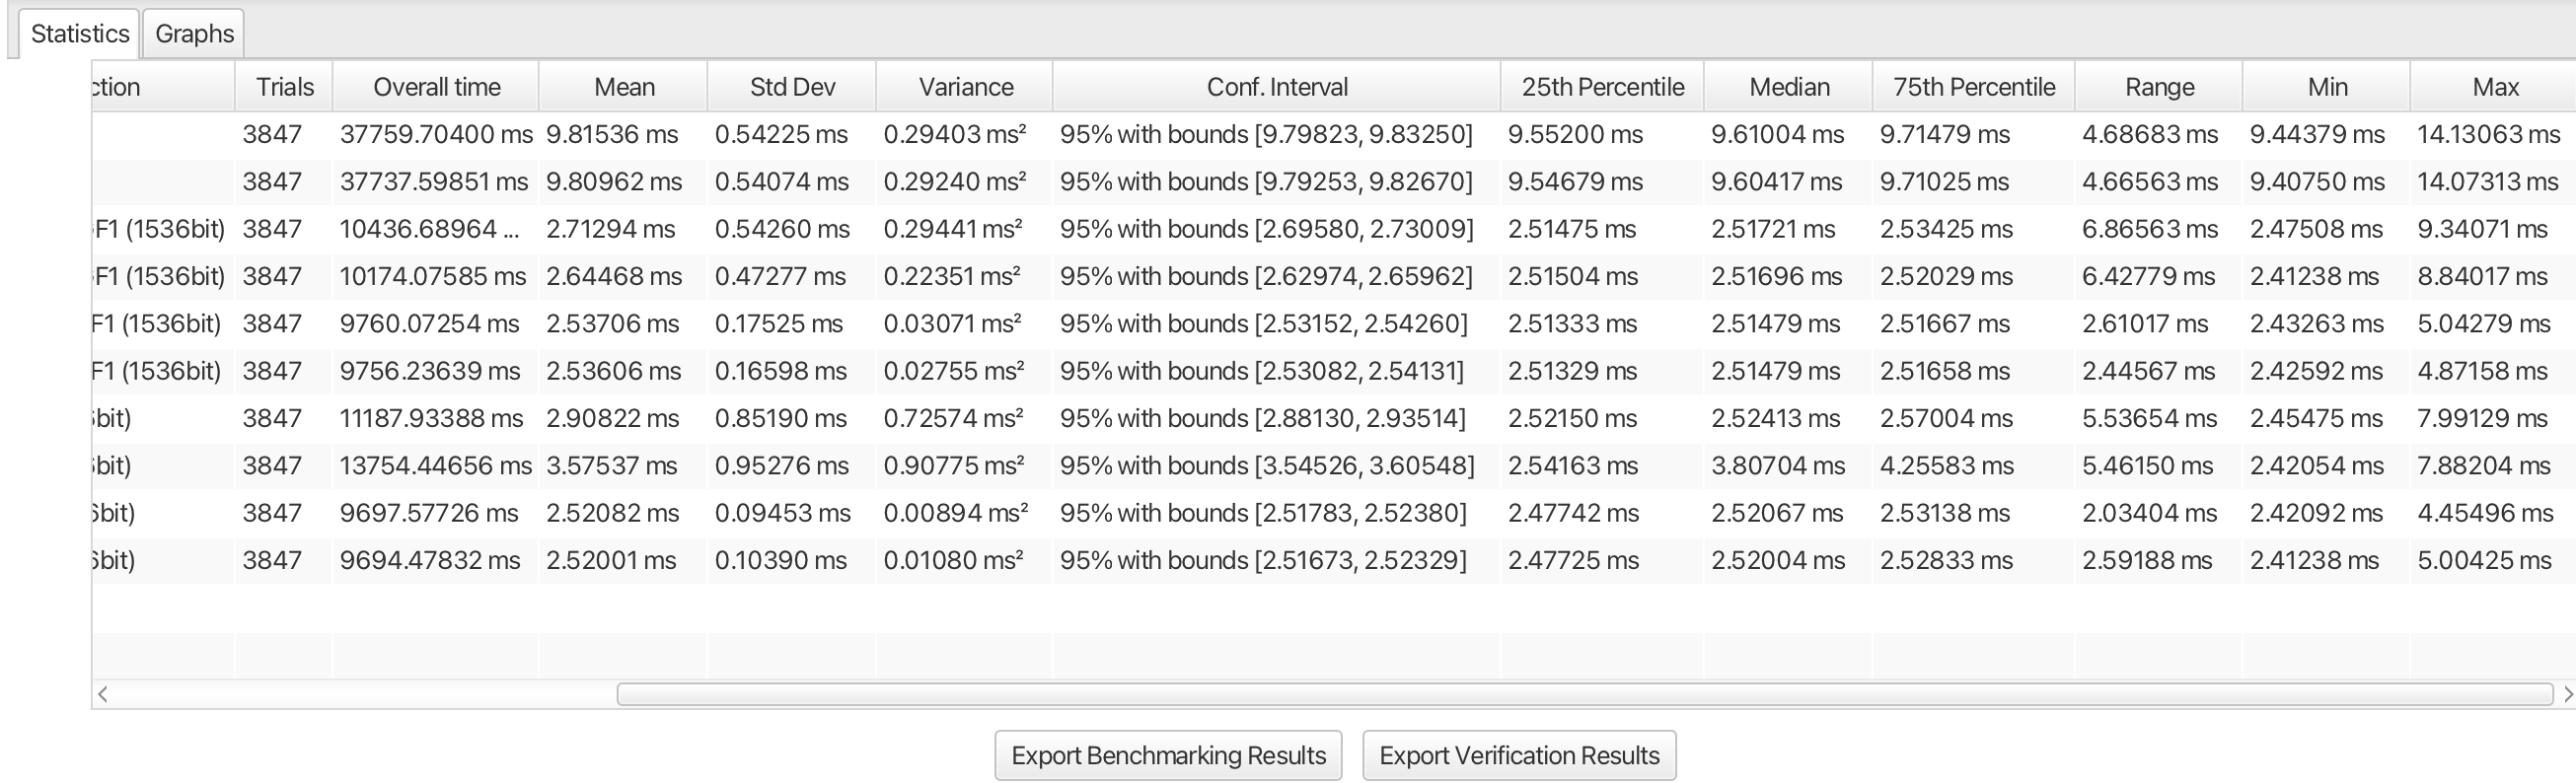
\includegraphics[width=\textwidth]{main_pictures/ansi/ansi_verify_3072bit_table2_1.png}}
    \end{minipage}
          \label{ansi_verify_3072bit_table}
\end{figure}

\begin{figure}[H]
    \centering % Center the images
     \caption{Instantiation of ANSI X9.31 rDSA with standard vs provably secure parameters (4096-bit Key Size) for signature verification}
    % First image in a minipage
    \begin{minipage}{\textwidth}
        \centering
        \fbox{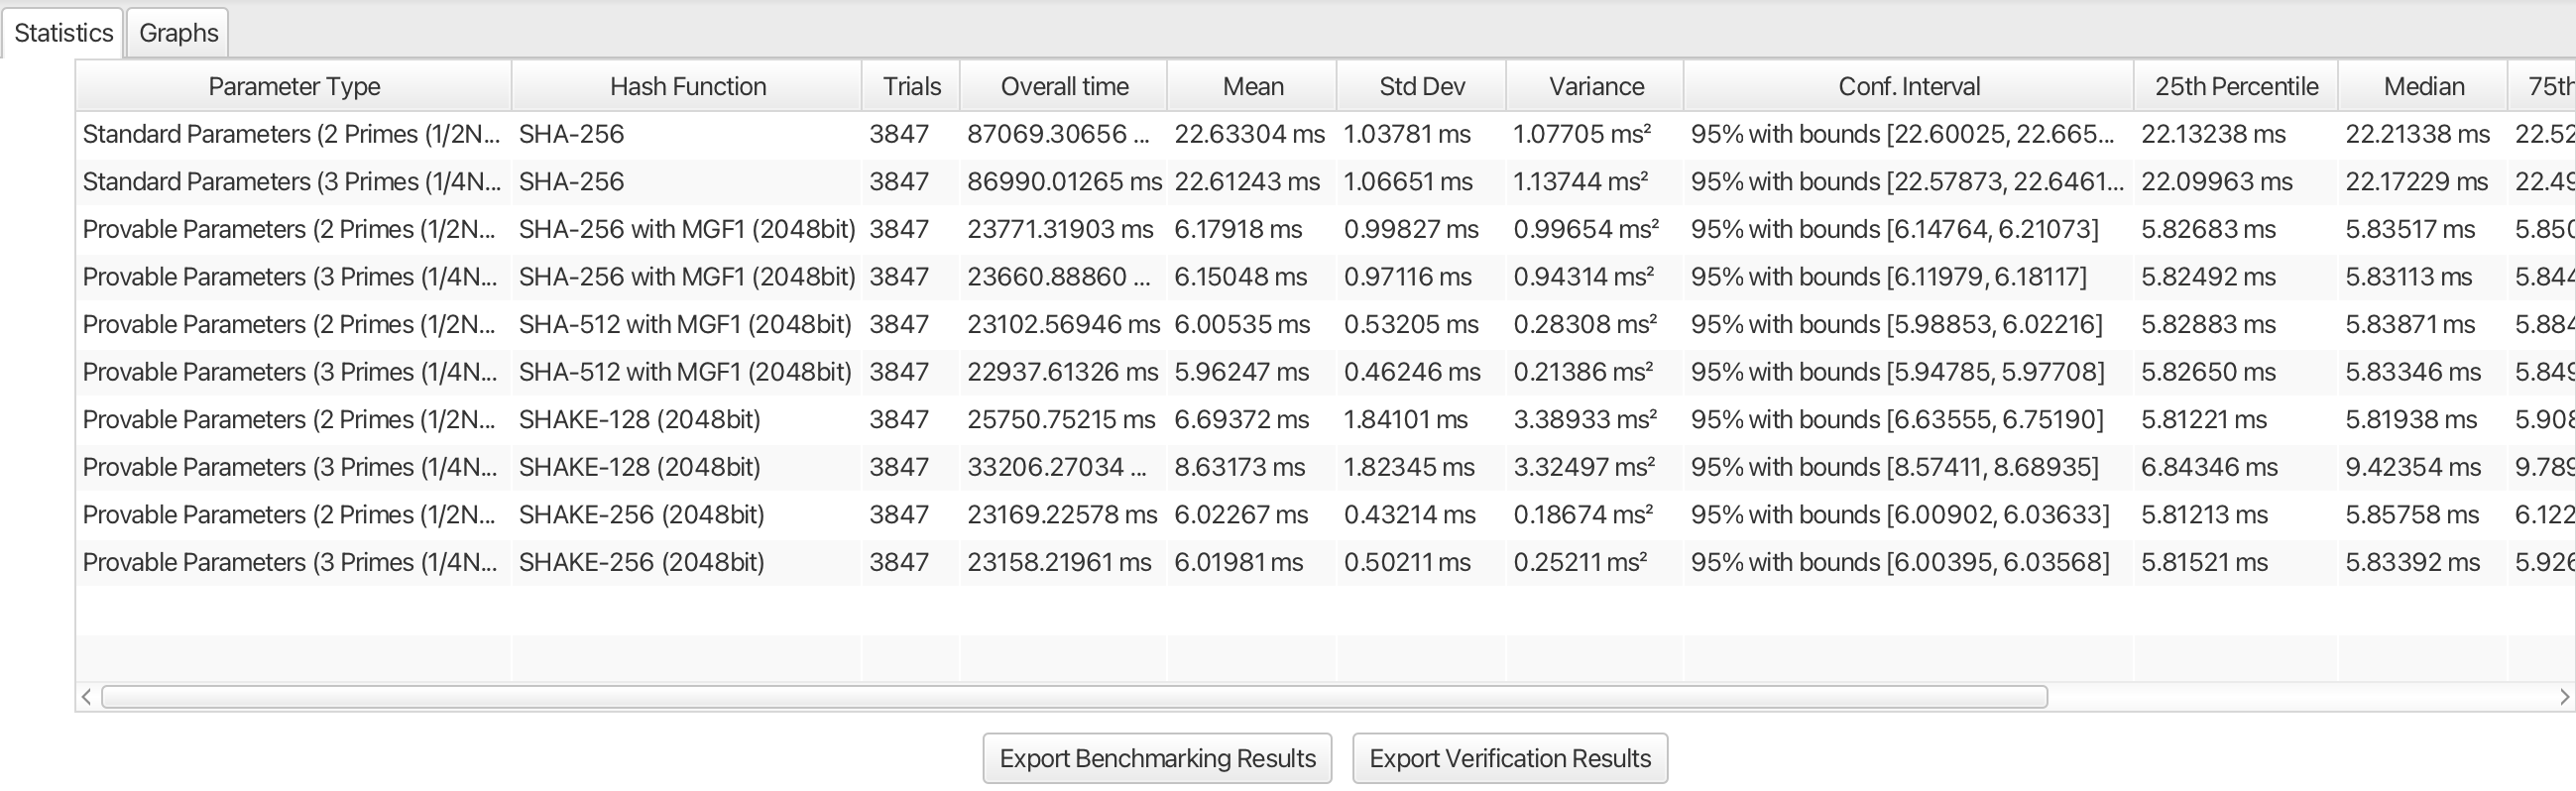
\includegraphics[width=\textwidth]{main_pictures/ansi/ansi_verify_4096bit_table1_1.png}} 
        \fbox{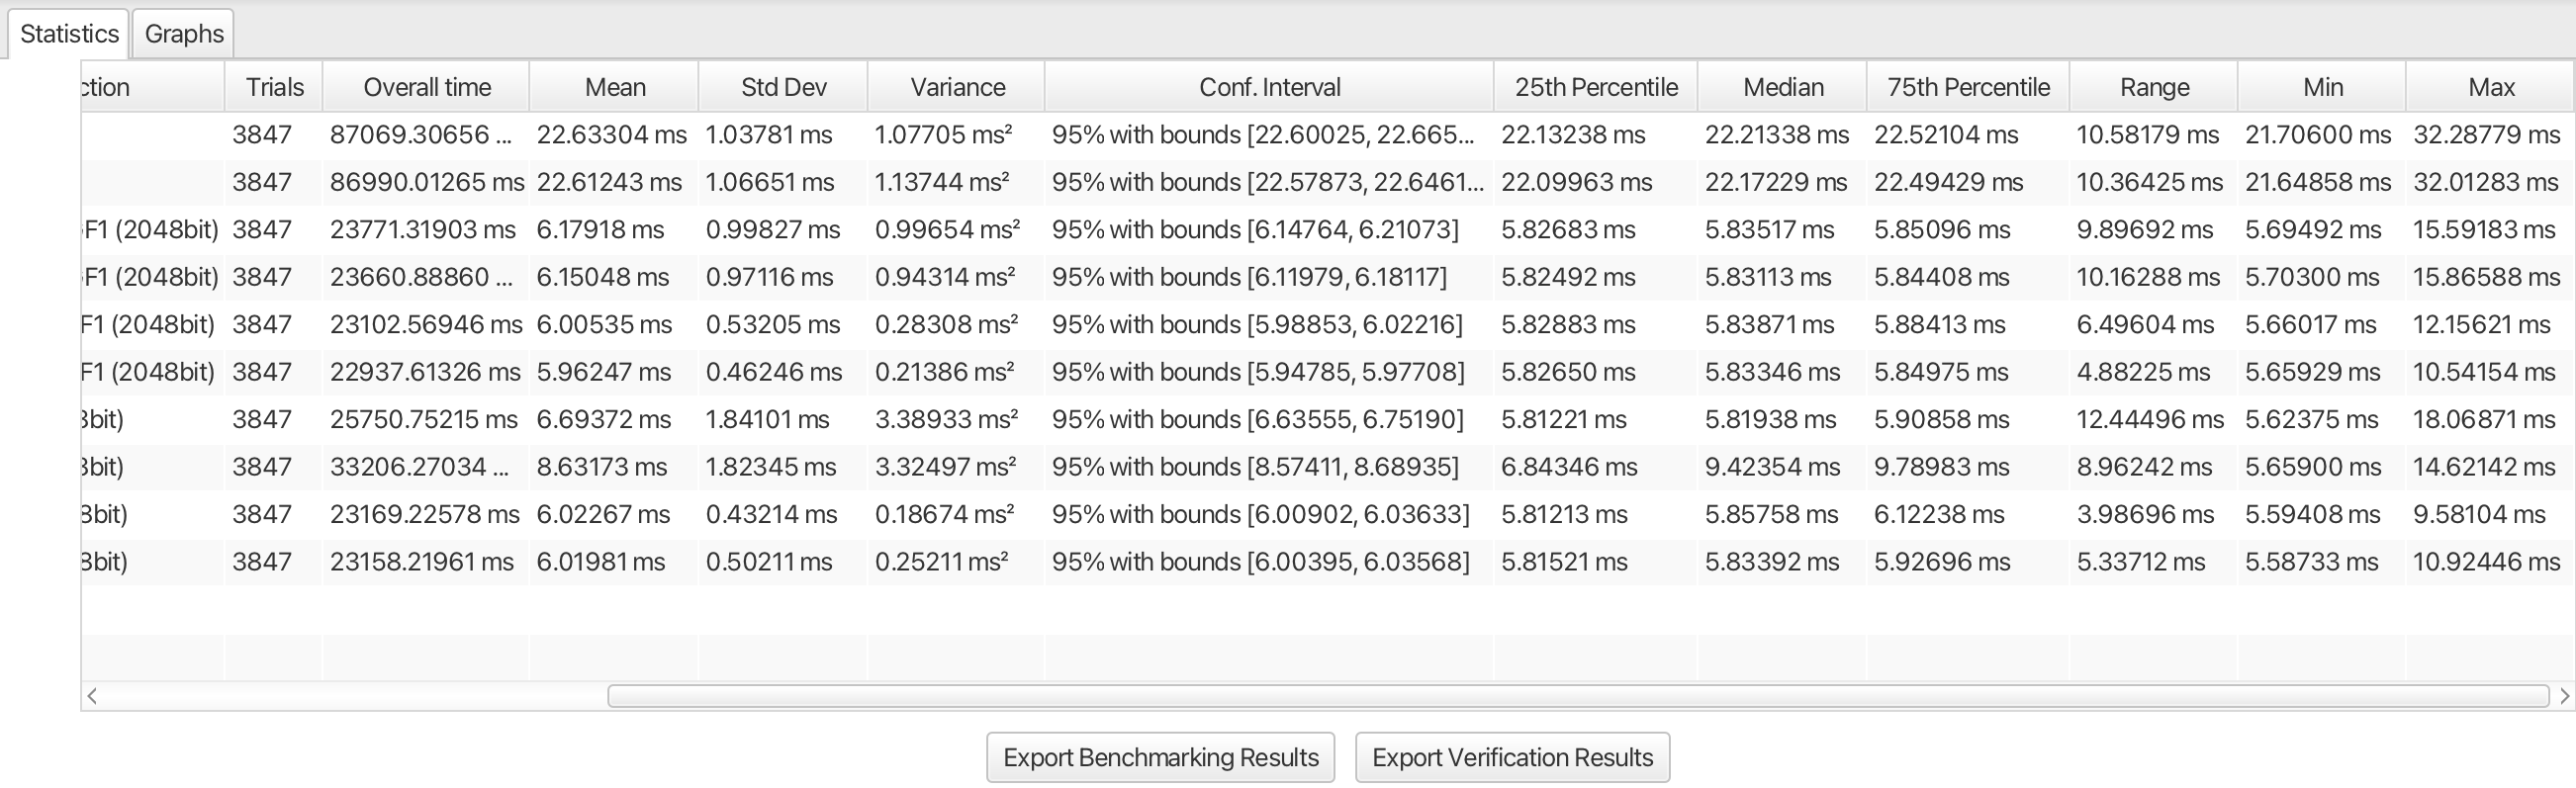
\includegraphics[width=\textwidth]{main_pictures/ansi/ansi_verify_4096bit_table2_1.png}}
    \end{minipage}
         \label{ansi_verify_4096bit_table}
\end{figure}

\begin{figure}[H]
    \centering % Center the images
     \caption{Instantiation of ANSI X9.31 rDSA with standard vs provably secure parameters (5120-bit Key Size) for signature verification}
    % First image in a minipage
    \begin{minipage}{\textwidth}
        \centering
        \fbox{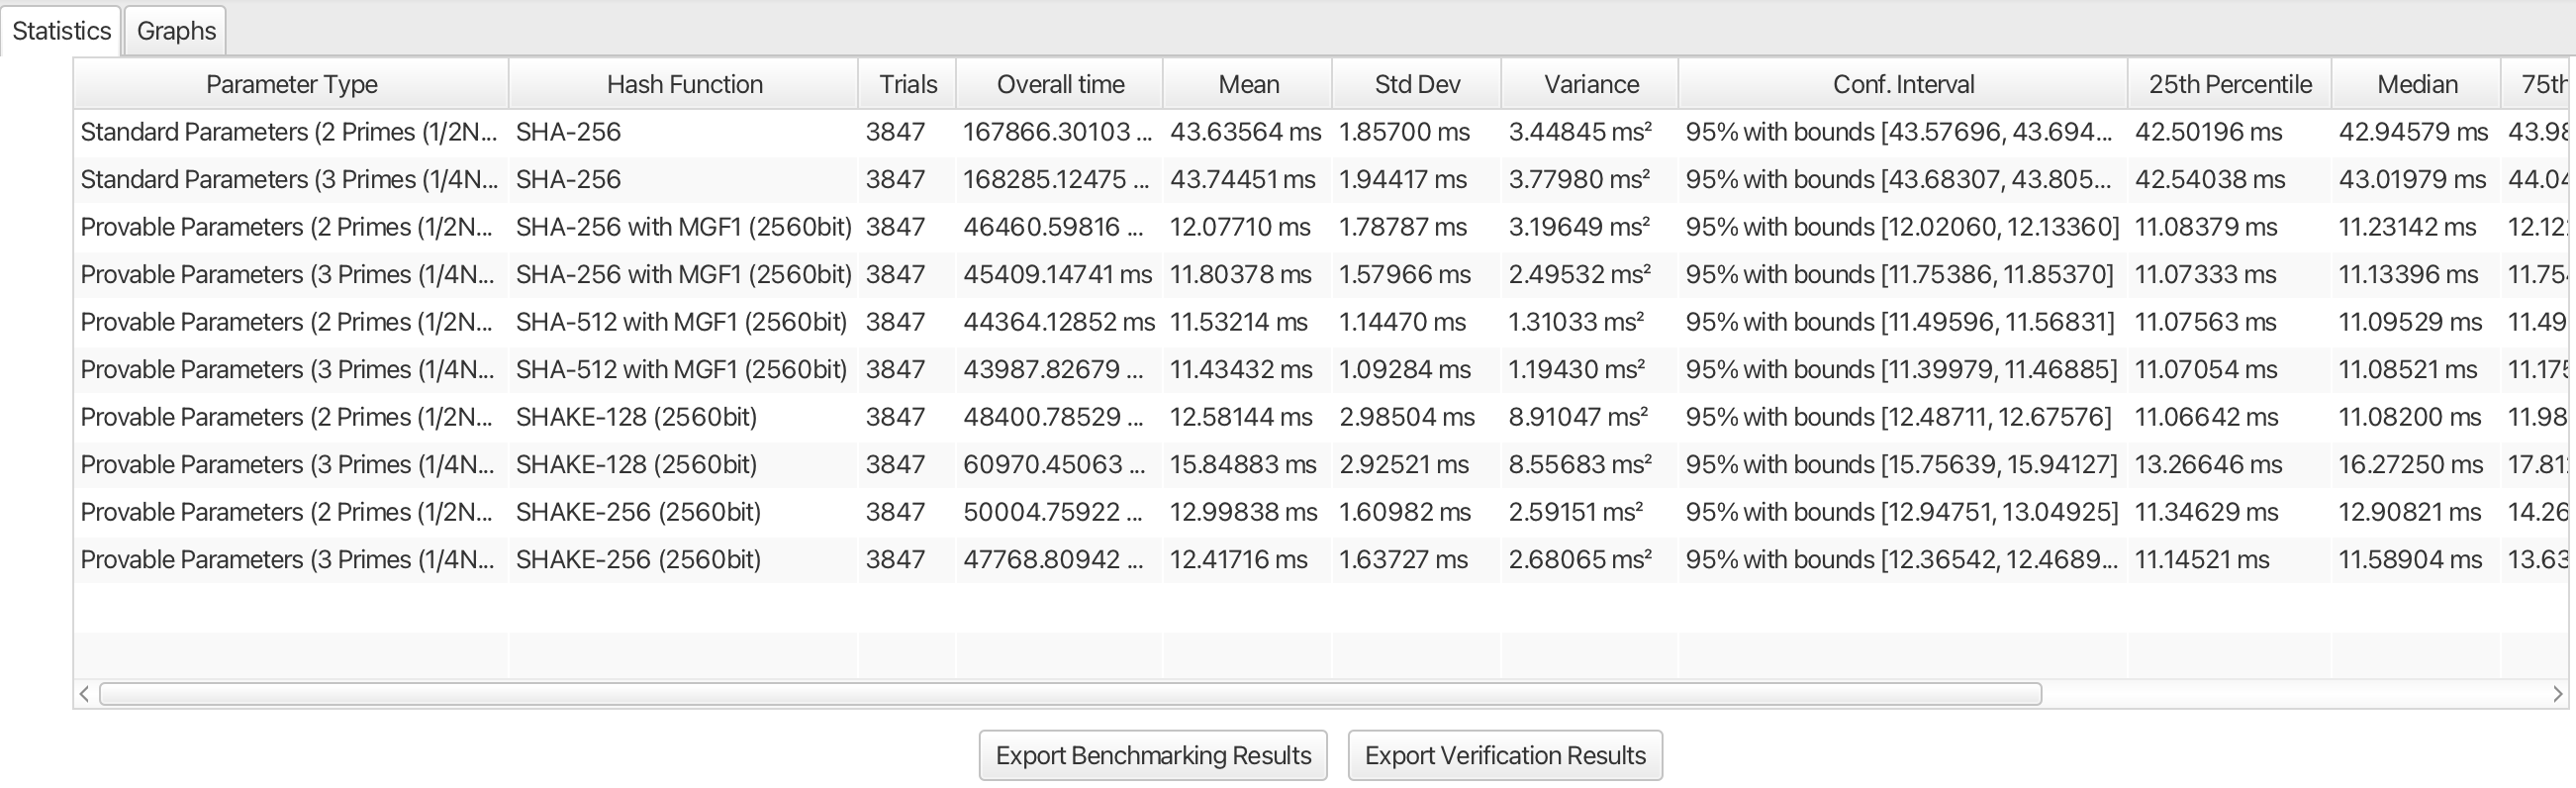
\includegraphics[width=\textwidth]{main_pictures/ansi/ansi_verify_5120bit_table1_1.png}} 
        \fbox{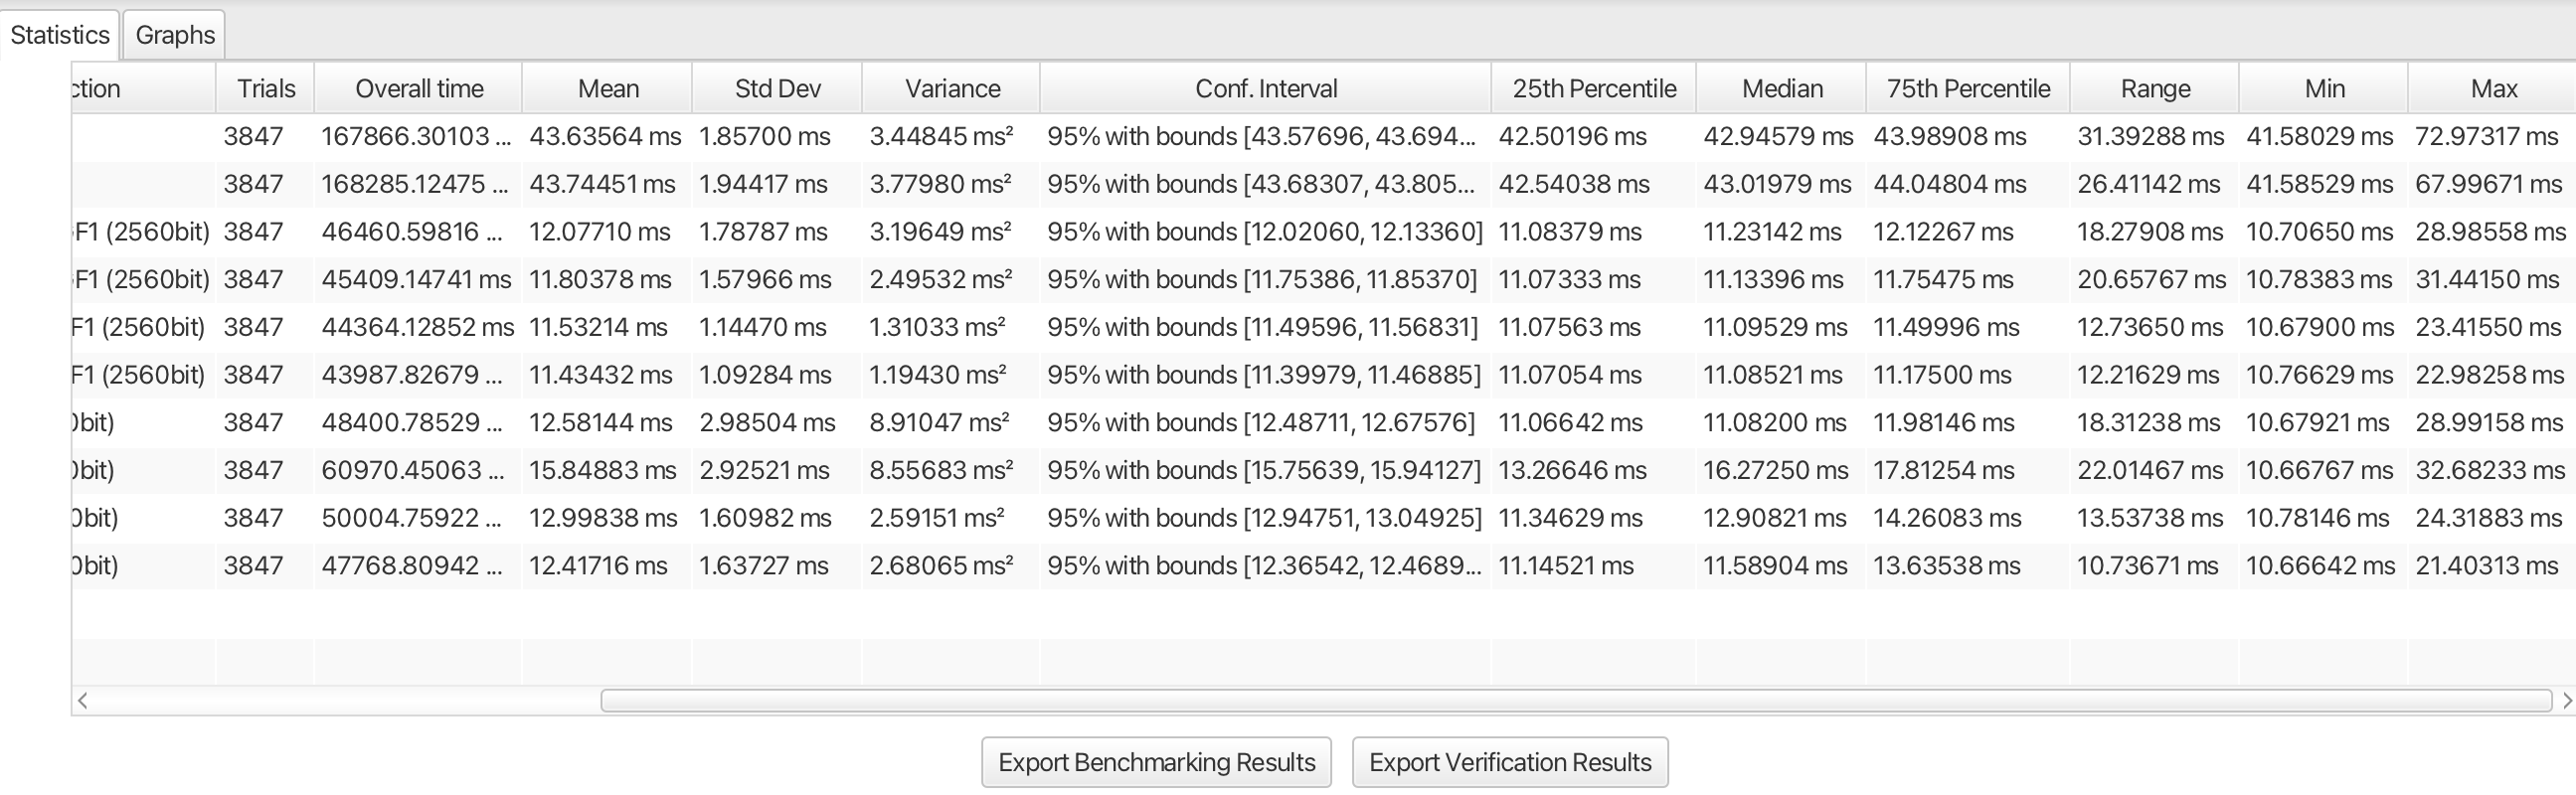
\includegraphics[width=\textwidth]{main_pictures/ansi/ansi_verify_5120bit_table2_1.png}}
    \end{minipage}
       \label{ansi_verify_5120bit_table}
\end{figure}

\begin{figure}[H]
    \centering % Center the images
     \caption{Instantiation of ANSI X9.31 rDSA with standard vs provably secure parameters (6144-bit Key Size) for signature verification}
    % First image in a minipage
    \begin{minipage}{\textwidth}
        \centering
        \fbox{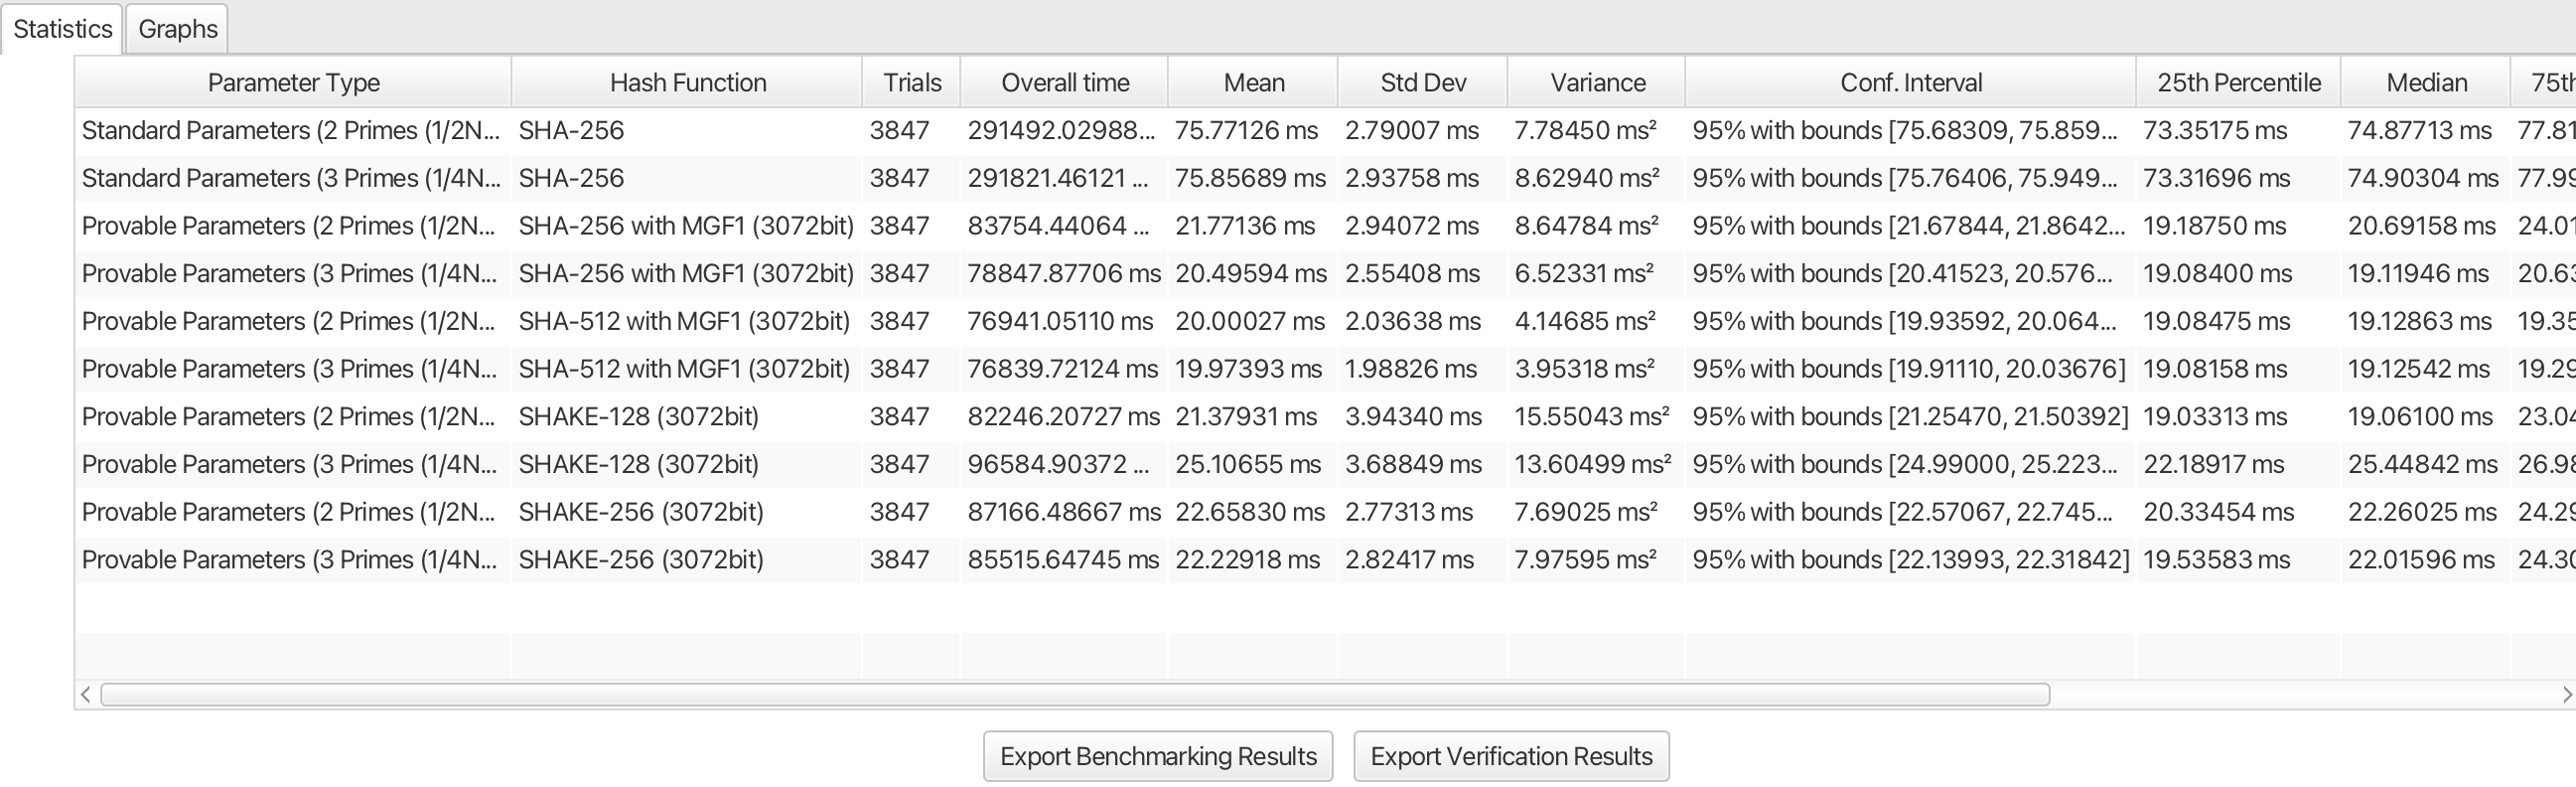
\includegraphics[width=\textwidth]{main_pictures/ansi/ansi_verify_6144bit_table1_1.png}} 
        \fbox{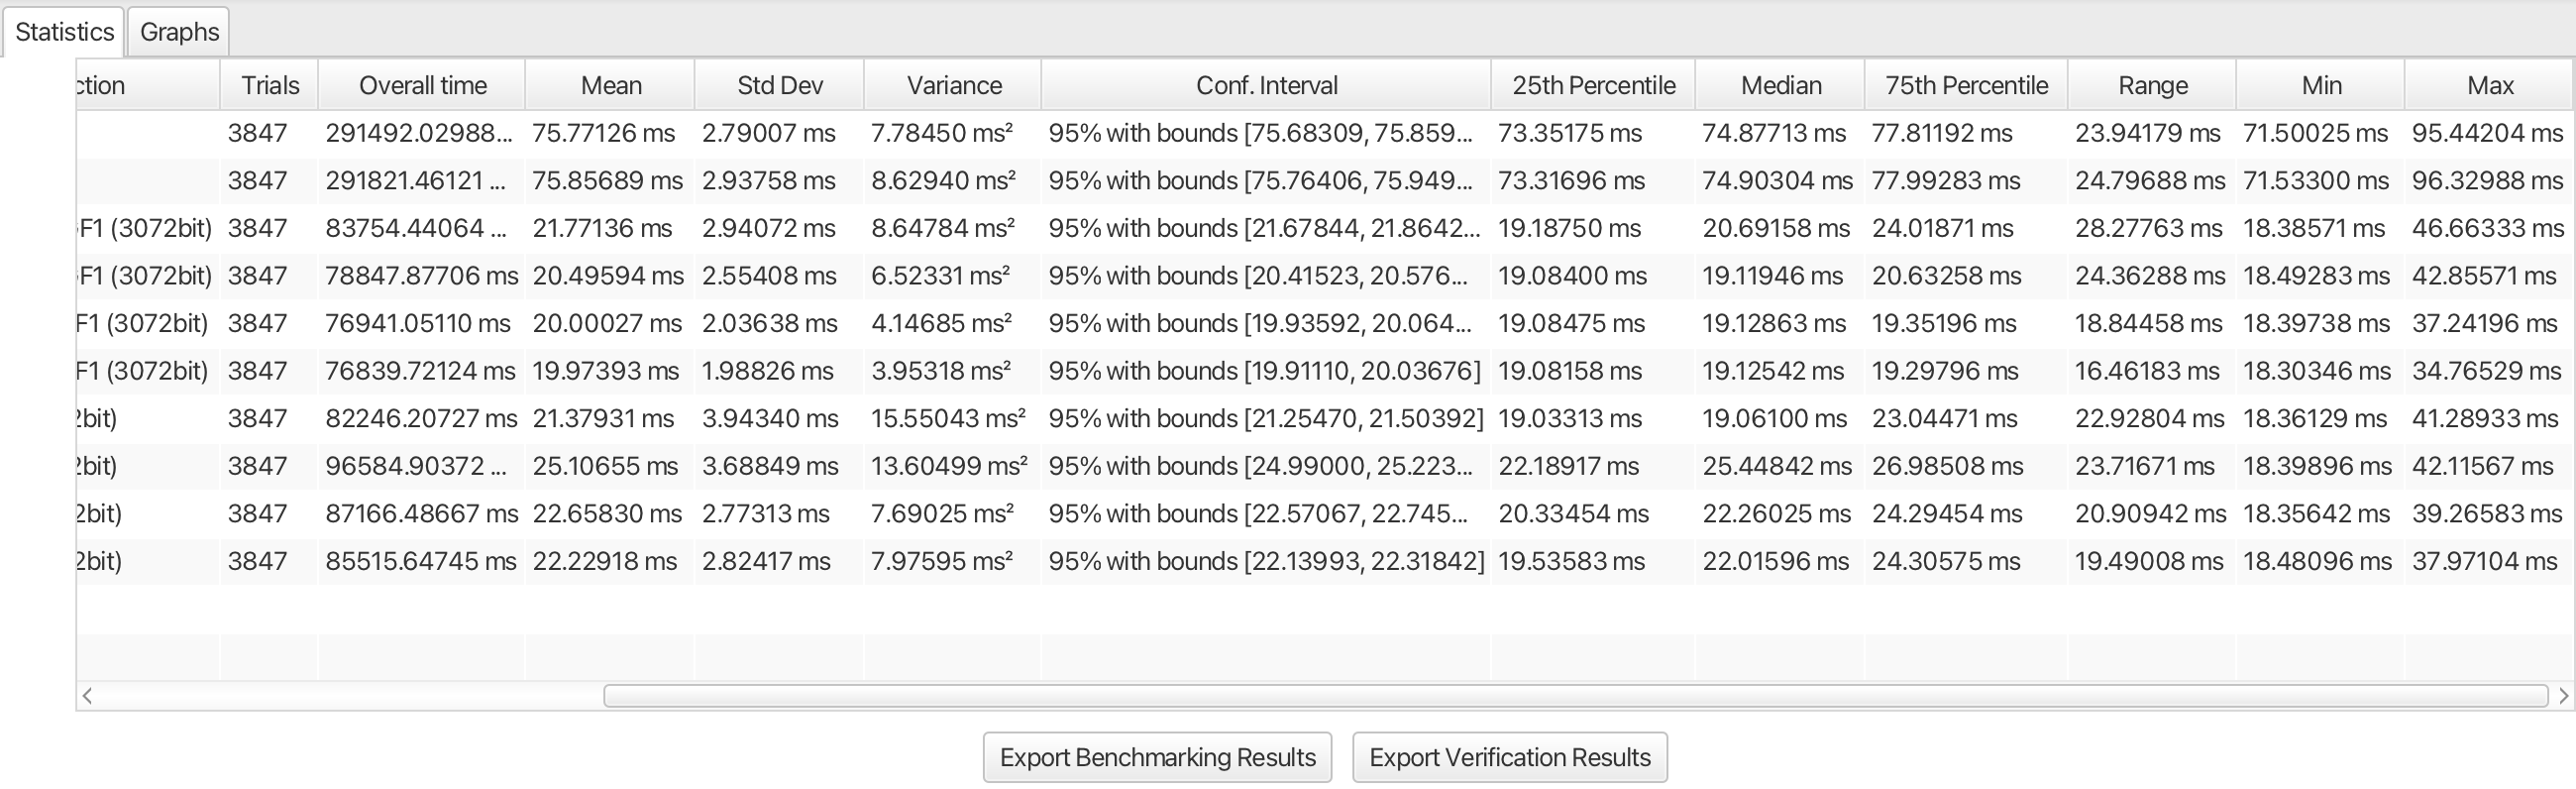
\includegraphics[width=\textwidth]{main_pictures/ansi/ansi_verify_6144bit_table2_1.png}}
    \end{minipage}
         \label{ansi_verify_6144bit_table}
\end{figure}



\subsection*{Standard Parameters}
\begin{itemize}
\item 2 Primes: Mean verification time with SHA-256 ranges from 0.48673 ms (1024-bit) to 75.77126 ms (6144-bit).
\item 3 Primes: Mean verification time with SHA-256 ranges from 0.48066 ms (1024-bit) to 75.85689 ms (6144-bit).
\end{itemize}

\subsection*{Provable Parameters (2 Primes)}
\begin{itemize}
\item SHA-512 with MGF1: Exhibits improvements in verification time compared to standard parameter instantiations with 2 Primes, with reductions ranging from 73.46\% to 75.56\%. This hash function also shows consistently lower variance compared to other provably secure parameter instantiations.
\item SHAKE-256: Shows considerable improvements in verification time compared to standard parameters with 2 Primes, with reductions ranging from 70.10\% to 75.57\%. It generally has lower variance across various key sizes.
\item SHA-256 with MGF1: Demonstrates significant improvement in verification time compared to standard parameters with 2 Primes, with reductions ranging from 70.13\% to 73.07\%. It displays moderately low variance, generally higher than SHA-512 with MGF1 and SHAKE-256.
\item SHAKE-128: Offers the smallest improvement in verification time compared to standard parameters with 2 Primes, ranging from 70.37\% to 72.83\%. However, it consistently has the highest variance among the provably secure parameter instantiations.
\end{itemize}

\subsection*{Provable Parameters (3 Primes)}
\begin{itemize}
\item SHA-512 with MGF1: Delivers improvements in verification time compared to standard parameters with 3 Primes, with reductions ranging from 73.63\% to 75.07\%. Similar to its performance with 2 Primes, it maintains low variance across key sizes.
\item SHAKE-256: Shows improvements in verification time compared to standard parameters with 3 Primes, with reductions ranging from 70.1\% to 75.57\%. Consistently exhibits one of the lowest variances.
\item SHA-256 with MGF1: Demonstrates improvement in verification time compared to standard parameters with 3 Primes, ranging from 69.5\% to 73.31\%. While its variance is moderately low, it is slightly higher than SHA-512 with MGF1 and SHAKE-256.
\item SHAKE-128: Provides the least improvement in verification time compared to standard parameters with 3 Primes, ranging from 61.83\% to 71.88\%, and consistently shows the highest variance.
\end{itemize}


\begin{comment}
For 2 Primes:
SHA-512 with MGF1: Improvements range from 73.46\% to 75.56\%.
SHAKE-256: Improvements range from 70.10\% to 75.57\%.
SHA-256 with MGF1: Improvements range from 70.13\% to 73.07\%.
SHAKE-128: Improvements range from 70.37\% to 72.83\%.
For 3 Primes:
SHA-512 with MGF1: Improvements range from 73.63\% to 75.07\%.
SHAKE-256: Improvements range from 70.70\% to 75.27\%.
SHA-256 with MGF1: Improvements range from 69.50\% to 73.31\%.
SHAKE-128: Improvements range from 61.83\% to 71.88\%.

\subsection{Signature Verification Results (ANSI X9.31 rDSA)}
\end{comment}



\section{Signature Verification Results (ISO/IEC 9796-2:2010 Signature Scheme 1)}

\begin{figure}[H]
    \centering % Center the images
     \caption{Instantiation of ISO/IEC 9796-2:2010 Signature Scheme 1 with standard vs provably secure parameters (1024-bit Key Size) for signature verification}
    % First image in a minipage
    \begin{minipage}{\textwidth}
        \centering
        \fbox{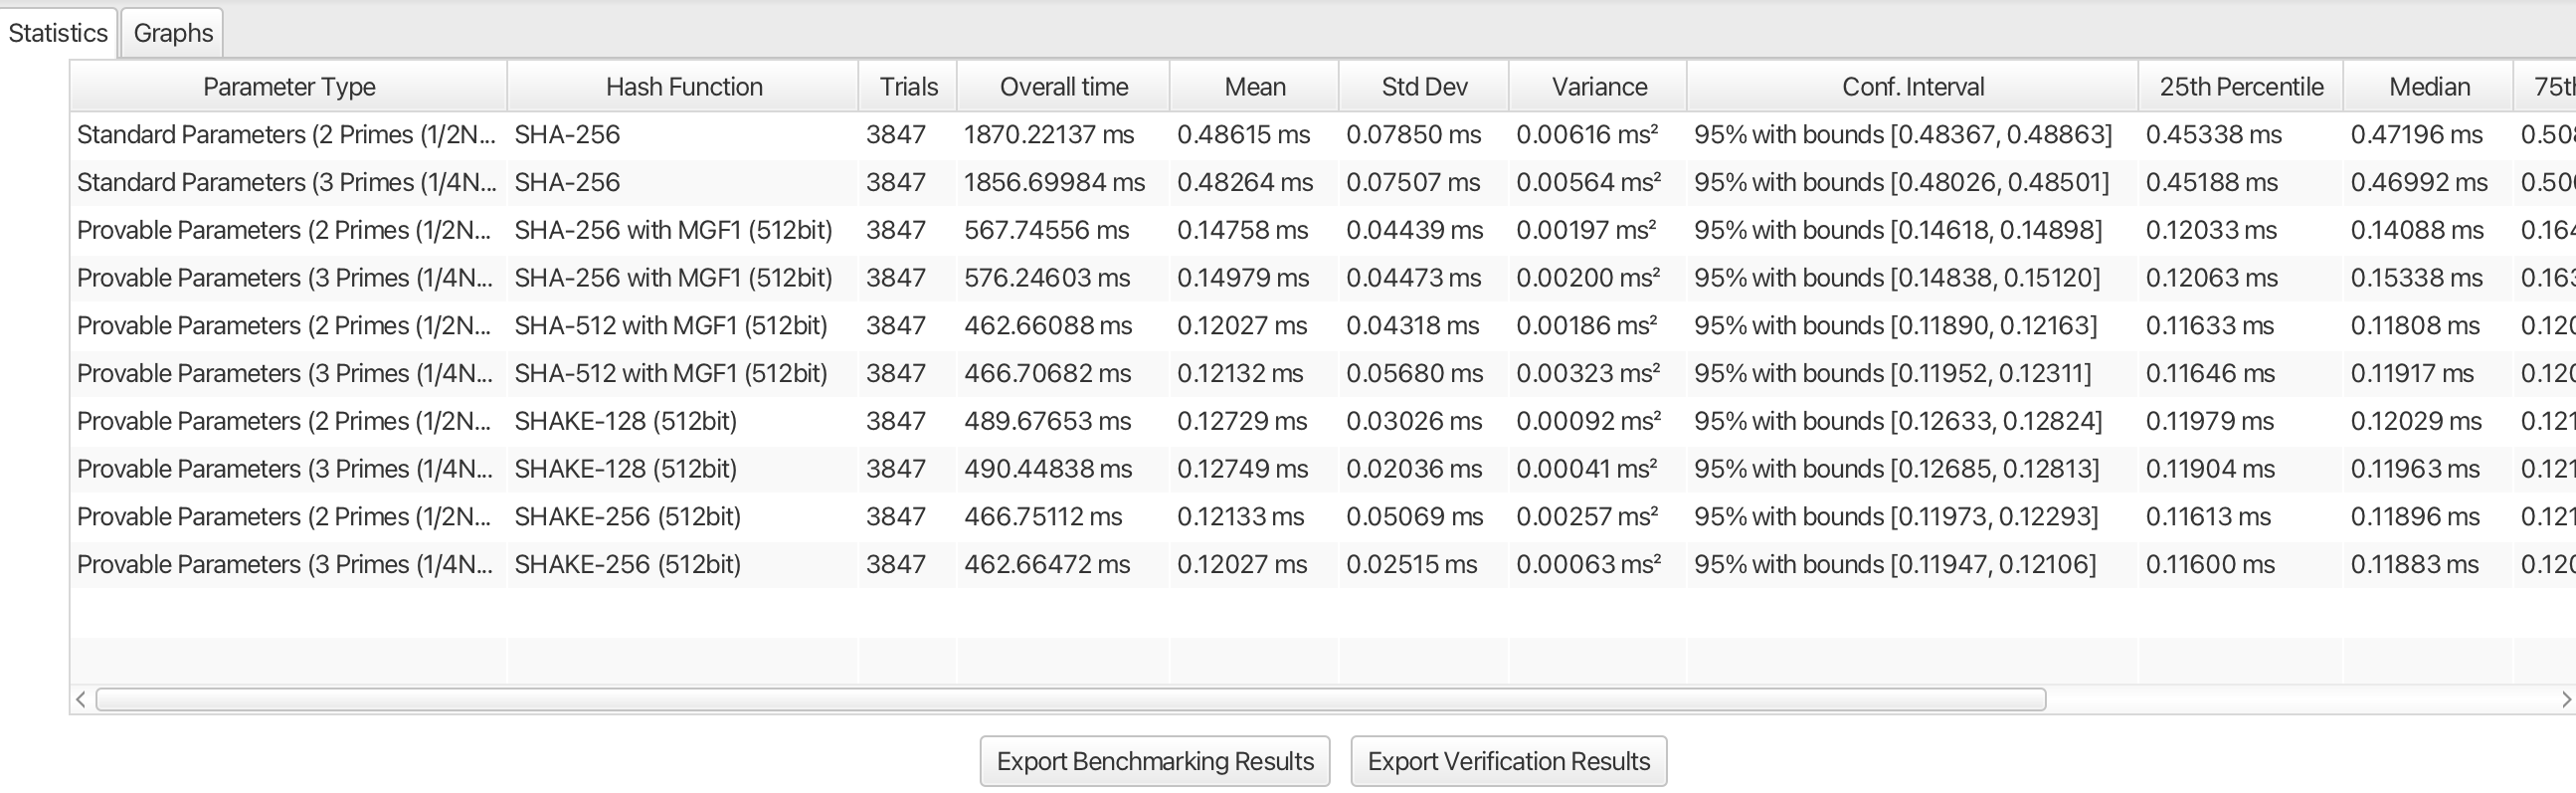
\includegraphics[width=\textwidth]{main_pictures/iso/iso_verify_1024bit_table1_1.png}} 
        \fbox{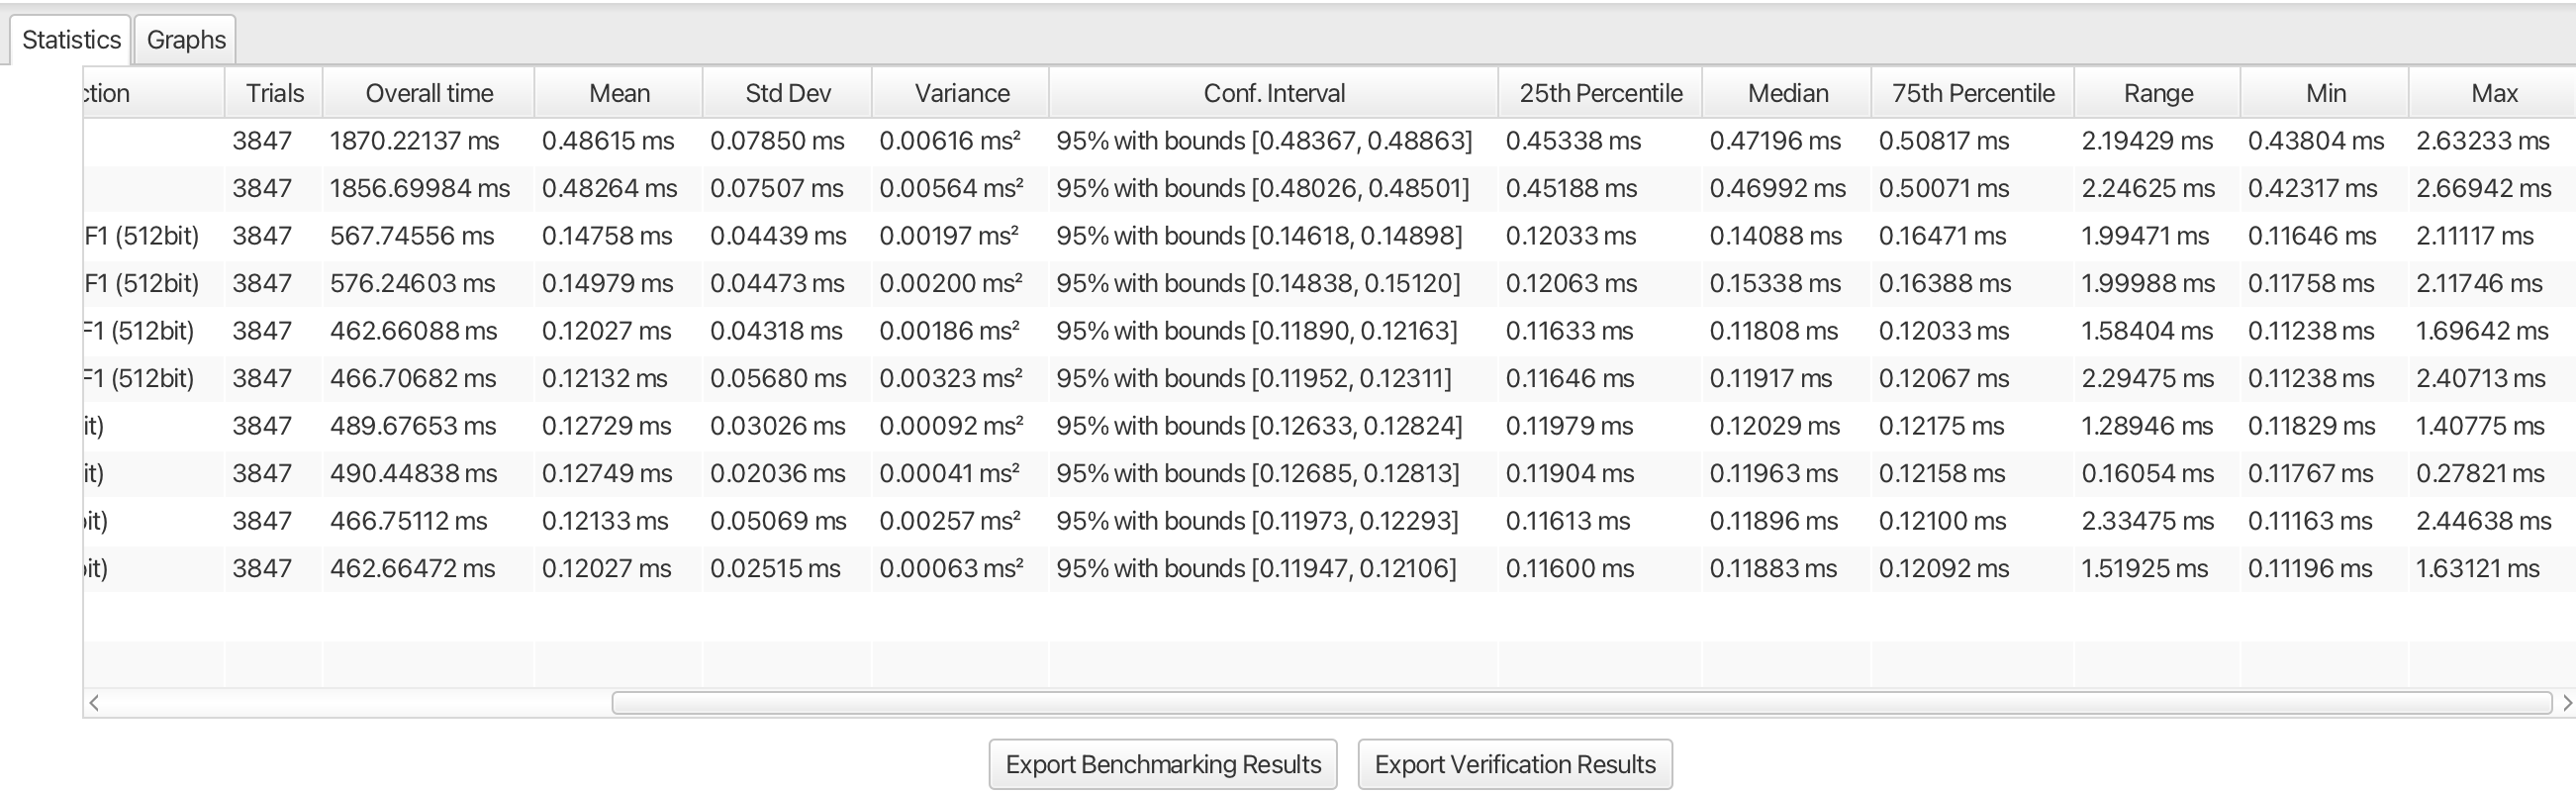
\includegraphics[width=\textwidth]{main_pictures/iso/iso_verify_1024bit_table2_1.png}}
    \end{minipage}
       \label{iso_verify_1024bit_table}
  \end{figure}
  
\begin{figure}[H]
    \centering % Center the images
     \caption{Instantiation of ISO/IEC 9796-2:2010 Signature Scheme 1 with standard vs provably secure parameters (2048-bit Key Size) for signature verification}
    % First image in a minipage
    \begin{minipage}{\textwidth}
        \centering
        \fbox{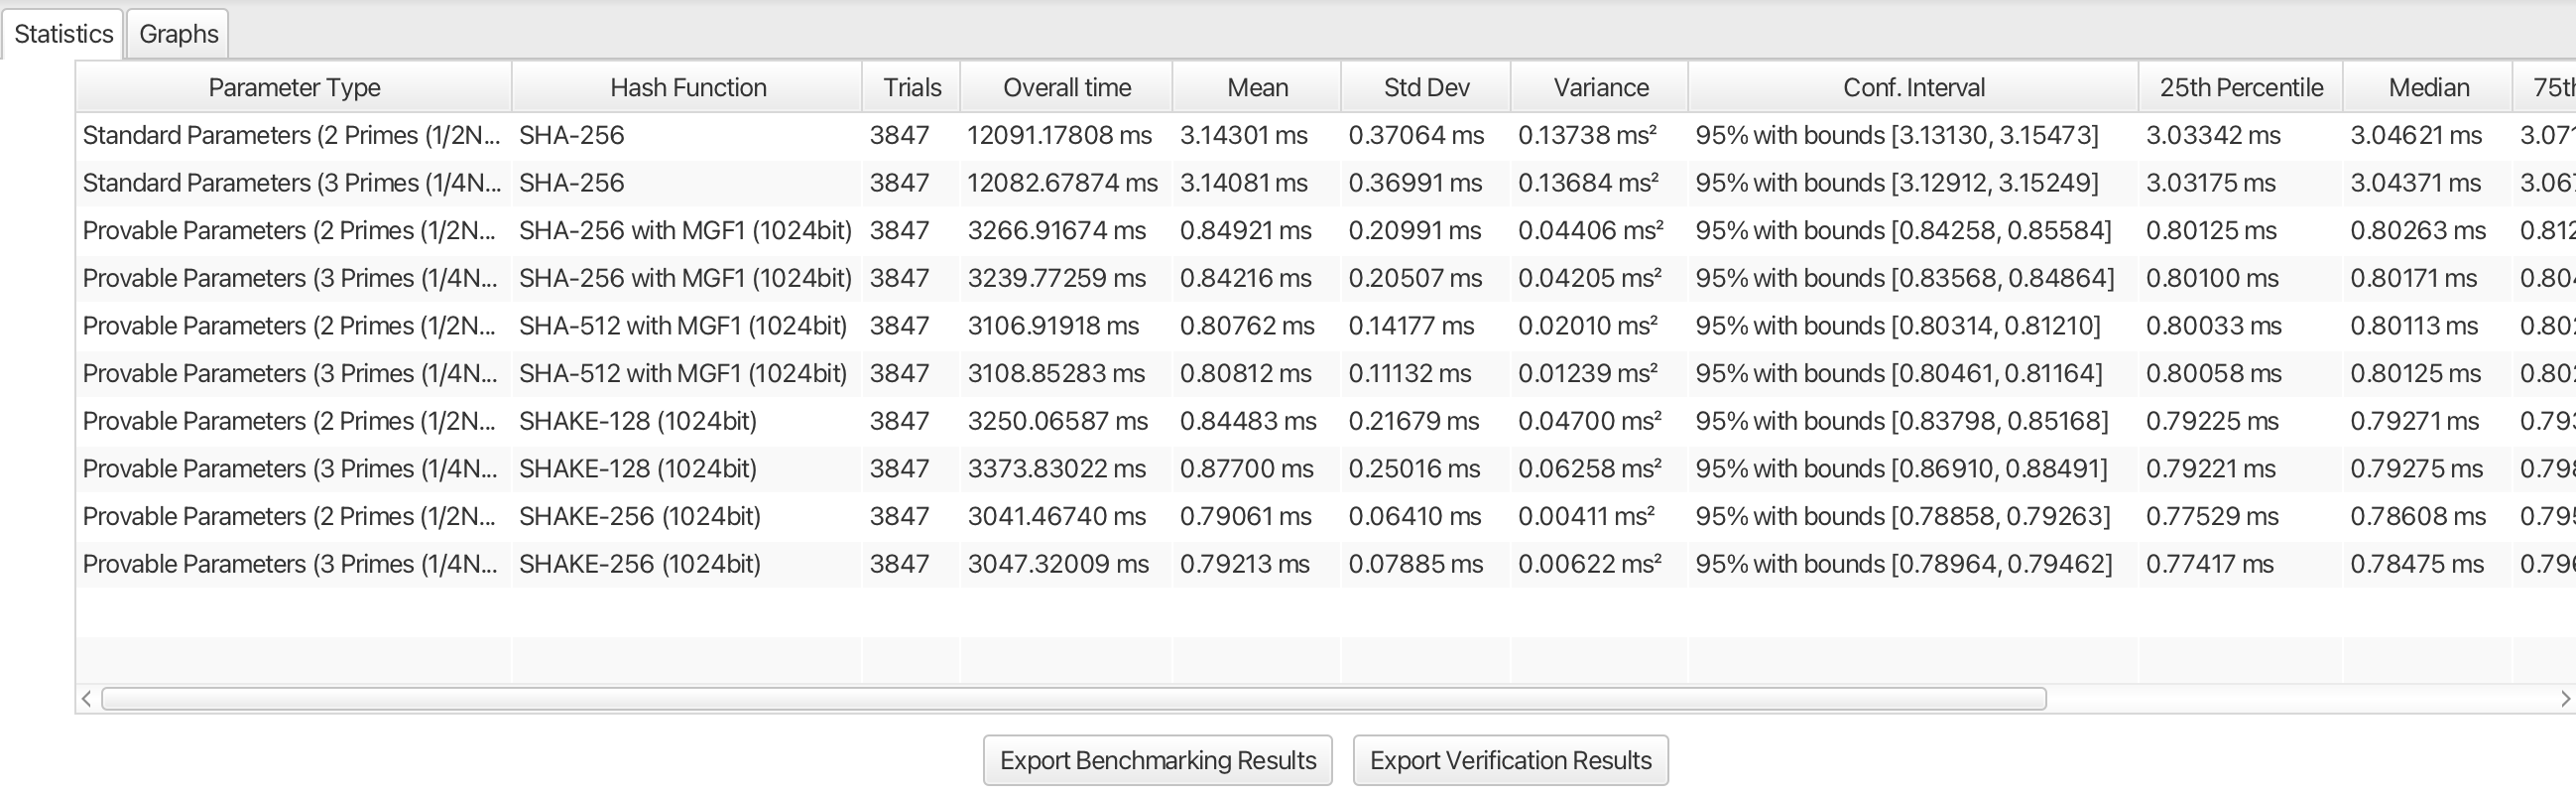
\includegraphics[width=\textwidth]{main_pictures/iso/iso_verify_2048bit_table1_1.png}} 
        \fbox{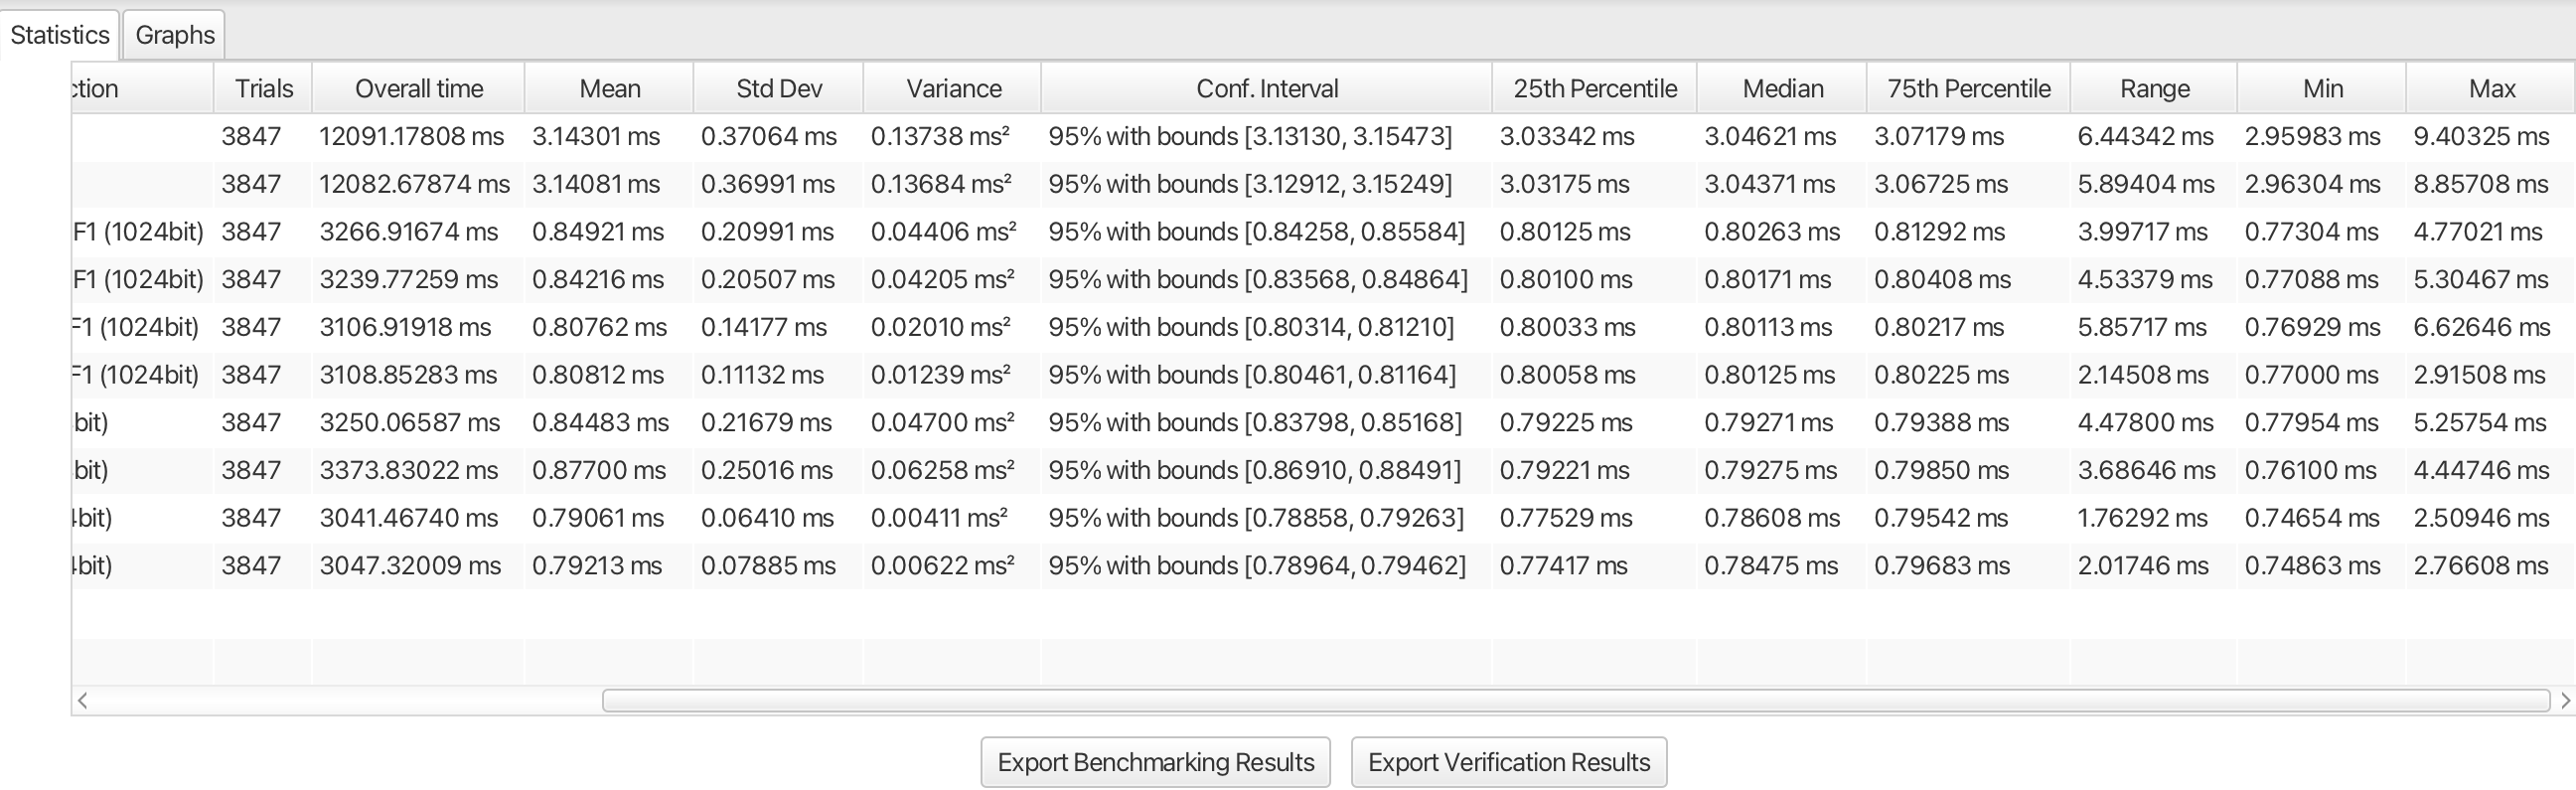
\includegraphics[width=\textwidth]{main_pictures/iso/iso_verify_2048bit_table2_1.png}}
    \end{minipage}
           \label{iso_verify_2048bit_table}
  \end{figure}
  
\begin{figure}[H]
    \centering % Center the images
     \caption{Instantiation of ISO/IEC 9796-2:2010 Signature Scheme 1 with standard vs provably secure parameters (3072-bit Key Size) for signature verification}
    % First image in a minipage
    \begin{minipage}{\textwidth}
        \centering
        \fbox{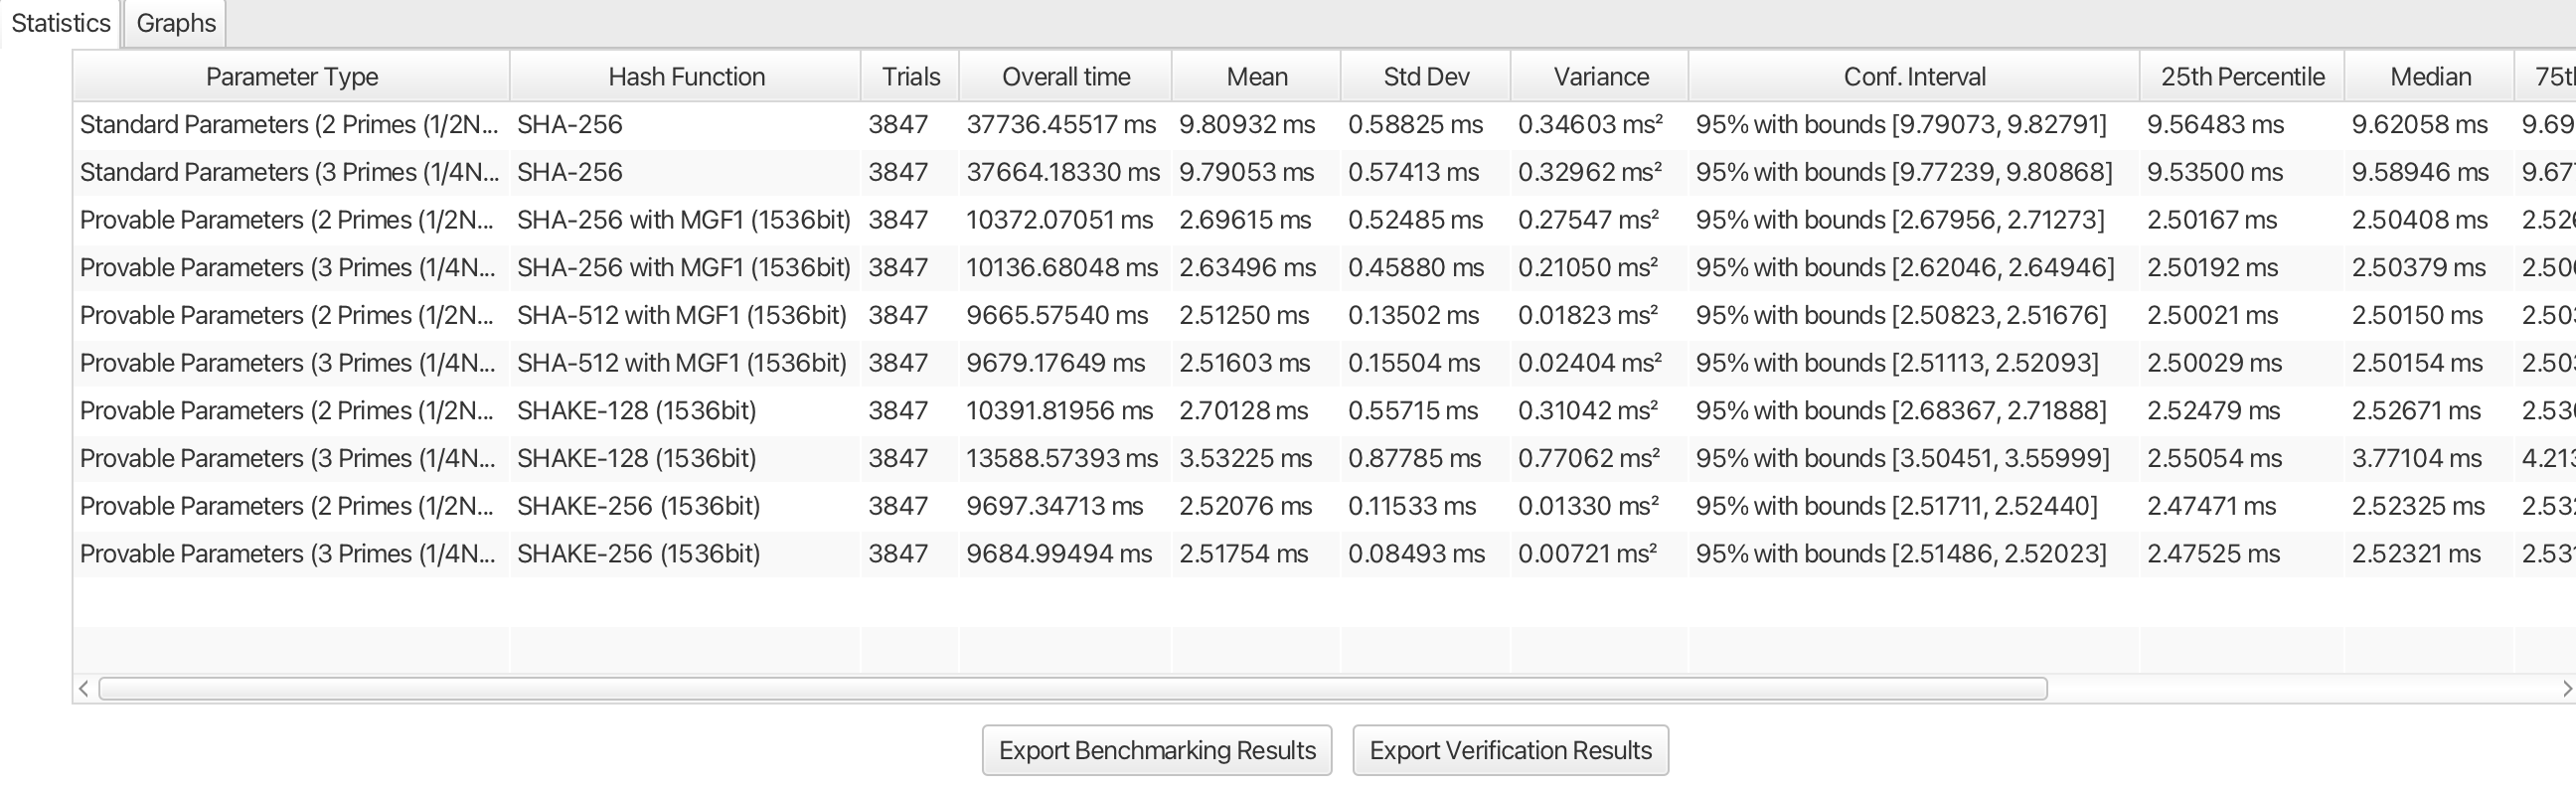
\includegraphics[width=\textwidth]{main_pictures/iso/iso_verify_3072bit_table1_1.png}} 
        \fbox{\includegraphics[width=\textwidth]{main_pictures/iso/iso_verify_3072bit_table2_1.png}}
    \end{minipage}
          \label{iso_verify_3072bit_table}
\end{figure}

\begin{figure}[H]
    \centering % Center the images
     \caption{Instantiation of ISO/IEC 9796-2:2010 Signature Scheme 1 with standard vs provably secure parameters (4096-bit Key Size) for signature verification}
    % First image in a minipage
    \begin{minipage}{\textwidth}
        \centering
        \fbox{\includegraphics[width=\textwidth]{main_pictures/iso/iso_verify_4096bit_table1_1.png}} 
        \fbox{\includegraphics[width=\textwidth]{main_pictures/iso/iso_verify_4096bit_table2_1.png}}
    \end{minipage}
         \label{iso_verify_4096bit_table}
\end{figure}

\begin{figure}[H]
    \centering % Center the images
     \caption{Instantiation of ISO/IEC 9796-2:2010 Signature Scheme 1 with standard vs provably secure parameters (5120-bit Key Size) for signature verification}
    % First image in a minipage
    \begin{minipage}{\textwidth}
        \centering
        \fbox{\includegraphics[width=\textwidth]{main_pictures/iso/iso_verify_5120bit_table1_1.png}} 
        \fbox{\includegraphics[width=\textwidth]{main_pictures/iso/iso_verify_5120bit_table2_1.png}}
    \end{minipage}
       \label{iso_verify_5120bit_table}
\end{figure}

\begin{figure}[H]
    \centering % Center the images
     \caption{Instantiation of ISO/IEC 9796-2:2010 Signature Scheme 1 with standard vs provably secure parameters (6144-bit Key Size) for signature verification}
    % First image in a minipage
    \begin{minipage}{\textwidth}
        \centering
        \fbox{\includegraphics[width=\textwidth]{main_pictures/iso/iso_verify_6144bit_table1_1.png}} 
        \fbox{\includegraphics[width=\textwidth]{main_pictures/iso/iso_verify_6144bit_table2_1.png}}
    \end{minipage}
         \label{iso_verify_6144bit_table}
\end{figure}






\subsection*{Standard Parameters}
\begin{itemize}
\item 2 Primes: Mean verification time with SHA-256 ranges from 0.48615 ms (1024-bit) to 75.18727 ms (6144-bit).
\item 3 Primes: Mean verification time with SHA-256 ranges from 0.48264 ms (1024-bit) to 75.36405 ms (6144-bit).
\end{itemize}

\subsection*{Provable Parameters (2 Primes)}
\begin{itemize}
\item SHA-512 with MGF1: Demonstrates improvement in verification time compared to standard parameter instantiations with 2 Primes, with reductions ranging from 73.70\% to 75.26\%. This hash function also shows consistently lower variance compared to other provably secure parameter instantiations.
\item SHAKE-256: Indicates improvement in verification time compared to standard parameters with 2 Primes, with reductions ranging from 70.12\% to 75.04\%. Generally, it exhibits lower variance across various key sizes.
\item SHA-256 with MGF1: Shows improvement in verification time compared to standard parameters with 2 Primes, with reductions ranging from 69.64\% to 72.98\%. Displays moderately low variance, which is generally higher compared to SHA-512 with MGF1 and SHAKE-256.
\item SHAKE-128: Offers the smallest improvements in verification time compared to standard parameters with 2 Primes, ranging from 73.39\% to 73.82\%. However, it consistently presents the highest variance among the provably secure parameter instantiations.
\end{itemize}

\subsection*{Provable Parameters (3 Primes)}
\begin{itemize}
\item SHA-512 with MGF1: Delivers improvement in verification time compared to standard parameters with 3 Primes, with reductions ranging from 73.72\% to 74.86\%. Similar to its performance with 2 Primes, maintains low variance across key sizes.
\item SHAKE-256: Shows improvement in verification time compared to standard parameters with 3 Primes, with reductions ranging from 70.34\% to 75.08\%. Consistently exhibits one of the lowest variances.
\item SHA-256 with MGF1: Demonstrates improvement in verification time compared to standard parameters with 3 Primes, ranging from 68.96\% to 73.19\%. Its variance is moderately low but is slightly higher than SHA-512 with MGF1 and SHAKE-256.
\item SHAKE-128: Provides the least improvement in verification time compared to standard parameters with 3 Primes, ranging from 62.14\% to 73.58\%, and consistently shows the highest variance.
\end{itemize}


\begin{comment}
\For 2 Primes:
* 		SHA-512 with MGF1: Improvements range from approximately 73.70\% to 75.26\%.
* 		SHAKE-256: Improvements range from about 70.12\% to 75.04\%.
* 		SHA-256 with MGF1: Improvements range from around 69.64\% to 72.98\%.
* 		SHAKE-128: Improvements range from approximately 73.39\% to 73.82\%.
For 3 Primes:
* 		SHA-512 with MGF1: Improvements range from approximately 73.72\% to 74.86\%.
* 		SHAKE-256: Improvements range from about 70.34\% to 75.08\%.
* 		SHA-256 with MGF1: Improvements range from around 68.96\% to 73.19\%.
* 		SHAKE-128: Improvements range from approximately 62.14\% to 73.58\%.
Specifically, the range of improvements in verification times when using provably secure parameters spans from 62.14\% to 75.26\%.



\end{comment}




\chapter{Appendix D Diary}

\section{Term 1}

\textbf{Diary Entry: Week of 18th - 24th September 2023}

This week was dedicated to writing a first draft of the abstract for my project (PKCS signature scheme) and researching arbitrary precision arithmetic for a library I may look to implement as part of the aims for the project

On Monday, I started writing about its importance, touching on its widespread use and history.
Tuesday was a continuation, emphasising why it's such a vital system.

By Wednesday, I added details on potential security issues, particularly focusing on something
called the Bleichenbacher attacks. I was initially puzzled about how these attacks affected the
signature scheme.

On Thursday and Friday, after more research, I figured out the difference between how these attacks
affect encryption and signature aspects of the system. This helped clarify some of my earlier
confusion.

Over the weekend, I added insights on why, despite some concerns, many still prefer the PKCS system.
I also touched upon a new research finding that supports its use. By Sunday, I detailed my main
goals for this project, hoping to create a useful tool that compares different signature schemes.

Next I will clarify whether I should consider implementing a self-made big number library as part of
the project and hopefully advance significantly in the creation of the project plan.

\textbf{Diary Entry - Week of 25th September - 1st October 2023}

Met with my supervisor for initial meeting. Discussed potential extensions to the original project
specifications and in general what the project entails. Refocused and refined the project plan,
emphasising deterministic RSA hash-and-sign schemes, especially PKCS\#1 v1.5. Made structural changes
to the introduction and abstract, enhancing clarity. Set up the Maven project directory on GitLab
and further developed the project timeline. Transitioned all documentation from Microsoft Word to
latex, drafting the literature review in the process. By week's end, automated referencing in latex
for enhanced efficiency.

\textbf{Diary Entry - Week of 2nd October - 8th October 2023}

This week, I refined and expanded the Risks and mitigation section, established a risk
quantification table, and deepened my understanding of digital signature schemes. The literature
review for the interim report was integrated, and significant progress was made in drafting the
cryptographic foundation of the report. By the weekend, focus was channeled into classifying digital
signature schemes and laying out a clear structure for detailed exploration of specific signature
schemes in upcoming sessions. Next I will begin writing the introductory section on digital
signatures for my report.

\textbf{Diary Entry - Week of 9th October - 15th October 2023}

I Started the week with supervisor meeting, confirming my focus on the POC PKCS Signature for term 1
and was given advice to potentially using the top 1000 English words for the signature program when
I sought guidance on the type of data I could provide to be signed. I delved into textbook RSA,
highlighting its vulnerabilities. By Friday, I had expanded on RSA's role in digital signatures,
introducing potential attacks and Hashed RSA signatures. The weekend saw me laying the foundation
for all three schemes considered in the project by formally defining them. I then began to explore
the motivation of provably secure signature schemes.

\textbf{Diary Entry - Week of 16th October - 22nd October 2023}

I started the week attempting to try and understanding trapdoor permutations, especially how they
tie into RSA. Following this I began work on enumerating the requirements for the proof of concept
program. By the end Friday, I had detailed the user stories and actors for the program with a
corresponding a UML use case diagram. During the weekend I first focussed on expanding the
motivation for provable security section with subsections on real world implications and
limitations. I finished off the week on Sunday by trimming down the report to make it more concise.

\textbf{Diary Entry - Week of 23rd October - 29th October 2023}

The week started with a meeting where I received constructive feedback on my project plan,
specifically that I had spent too much time on PKCS\#1 v1.5 encryption scheme and Bleichenbacher
attacks, which were deemed beyond the project’s scope. We clarified the implications of the interim
report's word limit, and I was reassured that my report’s structure was on the right track, though I
was advised against including full software design documents.

I primarily focused on refining my project plan based on feedback. After restructuring my report and
creating an appendix for the software requirements of the proof of concept program, I turned my
attention to conceptualising and beginning the implementation of the RSA key generation process,
culminating in a complete first draft by Friday. The weekend was dedicated to initiating a new
chapter on security proof in the report, laying down the foundational concepts and starting to weave
them into the project's larger narrative.

\textbf{Diary Entry - Week of 30th October - 5th November 2023}

Focused on enhancing the clarity and structure of my project report, I began by unifying the
background concepts for security proofs. I refined the introduction, dividing it into clear aims and
objectives. I then pruned excess information from several sections for brevity and clarity,
particularly around RSA concepts. I started work on the design phase for the proof of concept
program kicking off with a draft outline of the MVC architecture and factory patterns, which I later
formalised into a UML class diagram. By the week's end, I finalised design diagrams, integrated them
into the report, and refined the section on provable security. The upcoming weeks are now poised for
the implementation stage.

\textbf{Diary Entry - Week of 6th November - 12th November 2023}

This week, I had the 4th meeting with my supervisor, where we clarified the required content for the
security proofs in my report, focusing on the practical implications for the signature schemes. My
progress on the interim report was positively noted, and I announced my intention to submit a draft
shortly. I began conceptualising (Wednesday) and then coding the PKCS\#1 v1.5 signature scheme (
Thursday) with a focus on modularity. By the end of the week, I had not only implemented this scheme
but also completed the security proof chapter of my report, emphasising the implications for
practical parameter choices. I also improved the key generation process to be more parametrisable,
setting a foundation for term 2 work where this is required.

\textbf{Diary Entry - Week of 13th November - 19th November 2023}

This week, I focused on implementing various signature schemes, starting with conceptualising and
drafting the ANSI X9.31 signature scheme. Using Test-Driven Development, I developed and refined
this implementation, leveraging the modular code structure from the earlier PKCS scheme.

A significant part of the week involved troubleshooting and resolving issues related to signature
verification. In the ANSI implementation, legitimate signatures occasionally failed to verify. The
problem was traced to the message encoding method and was fixed by adjusting the first padding byte.

When implementing the ISO/IEC 9796-2 scheme, I encountered a similar issue with signature
verification failures. This time, it was due to the first padding byte causing the encoded message's
big integer representation to sometimes exceed the modulus size, leading to verification failures.
After thorough research and comparison with open-source implementations, I realised the necessity of
prepending an initial 0x00 byte to the encoded message array, a Java-specific implementation detail.

The week concluded with a substantial refactoring of the ISO scheme's class structure, simplifying
it to a single class that automatically adjusts the recovery mode based on the user's message
length.

\textbf{Diary Entry - Week of 20th November - 26th November 2023}

This week, I made substantial progress in both my report and the development of the proof of concept
program. I sent a draft of my report to my supervisor and rescheduled our meeting to Friday for
feedback. I then focused on developing models for the proof of concept program, beginning with the
key generation model and applying the state design pattern effectively. By midweek, I completed all
essential models for the program, setting the stage for controller development.

I then moved on to developing the program's views, ensuring they supported the observer design
pattern, and completed the implementation of all application views. After receiving positive
feedback and suggestions for minor improvements on my report from my supervisor, I advanced to
developing the controllers, completing the GenController and initiating the SignatureController.

Over the weekend, I finished the SignatureController, integrating it seamlessly with the views, and
developed the MainController to manage the application flow. The application was functionally
complete, albeit pending more rigorous testing. I concluded the week by reorganising the project and
code directory to better reflect the MVC pattern and separate different functional modules.


\textbf{Diary Entry - Week of 27th November - 3rd December 2023}

This week, I focused on finalising my project for the interim submission I started with integration
testing for the mainMenu and Sign view features using TestFX, ensuring the UI and
model-view-controller interactions worked correctly. By Tuesday, I had completed all integration
testing, including tests for the verify view, and updated the appendix with detailed test cases.

Midweek, I shifted to preparing my project presentation, developing introductory slides and key
concept overviews. During this period, I also enhanced the JavaDoc documentation across the project
and detailed the system testing results in the appendix.

On Friday, I create a new launch class for the application and generated a fat jar containing the
full application (with all classes and dependencies needed to run it). Additionally, I started
recording demo videos for the presentation and the final project submission.

Over the weekend, I put the finishing touches on the presentation slides and the demo videos. I also
updated the project's README with detailed run instructions and refined the report to incorporate
specifics from my implementation of the signature schemes.

Next, I will organise everything in a manner appropriate for the final submission and clean up any
remaining loose ends, ensuring that all elements of the project are polished.

\section{Term 2}

\textbf{Diary Entry - Week of 15th January - 21st January 2024}

This week was centred around preparing for the development of the more comprehensive Term 2
benchmarking program. I started with a supervisor meeting, receiving positive feedback on my interim
submission and noting that I could simplify the directory structure of my codebase, specific
requirements for the benchmarking program. My focus then shifted to researching and conceptualising
the implementation of MGF1 (Mask Generation Function 1) to meet the requirements in instantiating
the signatures with provably secure parameters for a large hash output. I updated the requirements
section of my report, redefining it for the more comprehensive benchmarking program and revising
user stories to encompass its expanded functionality. The week culminated in drafting a new UML use
case diagram and beginning to overhaul the design section to align with these new requirements.
Looking ahead, I plan to update other design diagrams and start adapting the lower level
implementation of the signature schemes for instantiation provably secure parameters.

\textbf{Diary Entry - Week of 22nd January - 28th January 2024}

This week, I focused on enhancing the key generation process and refining the signature schemes in
my project. I implemented the Mask Generation Function 1 (MGF1) and modified the key generation to
support provably secure parameters, particularly enabling a smaller 'e' value. I then refactored the
hash function integration within the signature schemes, adding support for SHA-512 and improving the
design for future extensibility and updated the pkcs scheme to allow instantiation with
these new parameters. By the end of the week, all signature schemes were adapted to be instantiated
with provably secure parameters. Additionally, I restructured the SignatureController. The refactor
involved creating a new interface for common view update operations and dividing the controller into
an abstract parent class for shared functionalities and distinct child classes for specific tasks in
signature creation and verification. This reorganisation aimed to enhance functionality and
maintenance, delineating shared and specific tasks for signature creation and verification.

\textbf{Diary Entry - Week of 29th January - 4th February 2024}

This week started with a productive meeting on Monday with my supervisor, where we discussed using
two or three primes for benchmarking and implementing provably secure parameters. I also received
guidance on integrating the MGF1 function. I then adjusted the MGF1 function within signature
schemes and got approval to use a third-party library for Keccak hashing.

On Tuesday and Wednesday, I focused on integrating benchmarking features into the key generation
module, adding a toggle switch for benchmarking mode and a user interface for inputting key
generation parameters.

By Thursday, I had created a benchmarking utility class to manage timing and computation of
statistical averages, along with a loading bar for visual progress representation.

On Friday, I designed a benchmarking results screen with tabulated layout and options for textual
and visual representation, and improved efficiency through multi-core processing.

Over the weekend, I structured the development and publication of benchmarking changes,
incorporating them into the genModel, and finalixing the BenchmarkingUtility class. Sunday was
dedicated to integrating these changes into the view assembly for key generation and finalixing
updates to the genModel.

\textbf{Diary Entry - Week of 5th February - 11th February 2024}

This week, my efforts concentrated on integrating benchmarking functionalities across the project,
focusing on both key generation and signature modules. I started by implementing a
createBenchmarkingTask method in the key generation controller for background processing and
observing user input for initiating benchmarking tasks. This was followed by resolving timing errors
due to concurrent task overlaps and refining the public/private key batch export process.

Midweek, I enhanced memory efficiency in key generation benchmarking using replacing futures with
CountDownLatch (to track the completion of all tasks within a trial) and began developing a results
module to calculate and display statistical metrics from benchmarking activities. In the signature
module, I integrated benchmarking features for signature creation, involving a parallelised method
for batch-signing messages and revamping the UI for batch operations. I also incorporated observer
methods in the Signature Creation controller for handling batch files.

By Friday, I had implemented a structured results module, designed to handle benchmarking results
effectively. This included a ResultsModel for calculating statistical metrics, a view for displaying
results, and a controller linking benchmarking activities to the results view through a
BenchmarkingContext helper class that is extended by each benchmarking activity (e.g., class
SignatureCreationContext extends BenchmarkingContext) and passed at point of construction to the
results controller, to enable it to display tailored options on the results view.

The week concluded with a focus on the signature verification module, implementing a parallelised
batch verification method and updating the UI to support batch operations. I set plans to conduct
integration tests, refine software design specifications for the application's transition to a
benchmarking focus, and alter the signing and verifying processes to allow user-selected hash
functions.

\textbf{Diary Entry - Week of 12th February - 18th February 2024}

I started with a supervisor meeting which led to a pivotal shift in my benchmarking approach,
transitioning from batch-based to individual key-based results. This change led me to rework the
batch methods in my application for accurate individual task timing and to reorganise the signature
collection process for correct verification. I also gained clarity on using hash IDs with the MGF1
function in different signature schemes, particularly in adapting the ANSI standard (the ANSI
standard is outdated and does not specify how to handle hash ID when applying the MGF1 to fixed hash
function).

Later on in the week I worked on enabling the choice of different hash functions in the signature
schemes (switching from an initial the hash map of hash IDs to storing hash IDs and static final
fields for efficiency) and adjusting the signature model to track hash types and sizes. This
required updates to the signing and verification interfaces, allowing users to select hash
functions, and modifying the Signature Controller to handle these changes.

A challenge arose with discrepancies in timing due to parallel processing. To resolve this, I
switched to sequential batch methods, ensuring precise timing. The week ended with me adapting the
results controller for managing per-key results and refactoring the signature schemes with a new
getHashID method for more efficient operations (as alluded to previously). I also added a consistent
footer across all application screens to unify the user interface.

\textbf{Diary Entry - Week of 19th February - 25th February 2024}

This week, my project saw substantial enhancements in both functionality and user interface. I
introduced a toggle switch across the application screens to switch between standard and
benchmarking modes, offering users more flexibility. To address the challenges with concurrent
execution in benchmarking, I reverted to synchronous methods for key generation, signature creation,
and verification.

A significant development was the initiation of a cross-parameter comparison benchmarking mode. This
involved upgrading the ResultsView for displaying results for multiple parameter types/keys in one
table for comparison and extensively refactoring the ResultsController for this new mode, along with
integrating support into the GenController.

In the latter part of the week, I focused on finalising the cross-parameter benchmarking
implementation. This required adapting the Key generation controller to preload keys pre-load keys
into signature related controllers if the generated key batches/individual key pairs are all
provably secure or keys were generated using cross parameters comparison mode. I then refactored the
signature controller assembly to support this new mode. Functionalities for resetting preloaded key
parameters and exporting verification results for cross-parameter benchmarking were also developed.

Additionally, I enhanced the non benchmarking mode for key generation so that user is presented with
an option on whether to use a small e in the generation of key and then refined the
SignatureController to include functionality for preloading a single key for non benchmarking mode
if key chosen is provably secure i.e., small was used to generate it.

Over the weekend, I concentrated on resolving errors and bugs emerging from the integration of the
new benchmarking mode, such as fixing crashes in signature views. I also dedicated time to
refactoring, streamlining the initialisation process for the different modes to enhance the
application's efficiency and user experience.

\textbf{Diary Entry - Week of 26th February – 3rd March 2024}

I started by updating the results view to include multiple graph representations, such as
histograms, box plots, and line graphs, tailored especially for comparing mean times in different
result sets. This update required substantial enhancements to the data processing backend, which I
completed successfully.

The integration of the fully-functional results graph feature into the main branch marked a
significant milestone. Building on this, I initiated the development of the
customCrossParameterBenchmarkingMode, a feature allowing users to specify precise key/parameter
configurations for benchmarking in comparison mode. This involved modifying the GenModel to handle
user-defined configurations and introducing new methods for generating readable string formats for
these custom configurations. Additionally, I implemented a toggle switch in the key generation view
and introduced dialog interactions for user input of configurations as multiple comma separated fractions.

Further refining the Signature model, I enabled the setting of a generalised number of key
configurations per key size for use in batch generation methods for comparison mode. I also enhanced
the ResultsController to dynamically construct an aggregated results table in comparison mode,
introducing a parameterised list for context-specific row headers based on previous benchmarking
tasks.

The latter part of the week saw me wrapping up the refactoring of the SignView and VerifyView domain
objects by creating a unified SignatureBaseView class. This significantly reduced code duplication
and streamlined handling across different signature views. I then conceptualised a new feature:
Multi-Hash Function Selection for Cross-Parameter Benchmarking, focusing on the specification and
management of custom key configurations.

By the weekend, I had developed a preliminary implementation of this feature, though it required
further refinement due to some bugs. By Sunday, I had completed significant enhancements across the
project to fully incorporate the Multi-Hash Function Selection feature, enabling the specification
and management of custom key configurations and grouping them to be used with selected hash
functions.

\textbf{Diary Entry - Week of 4th March – 10th March 2024}

This week, I focused on refining various aspects of my project, from bug fixes to significant
restructuring. Starting with resolving an issue in GenView and a benchmarking display error on
Monday, I then introduced the ability to specify custom hash output sizes for variable-length hash
functions in comparison mode on Tuesday. This involved notable changes across the application,
including a major refactoring of the KeyConfigurationsDialog from a lengthy method in GenView into a
more manageable KeyConfigurationsDialog class.

Midweek, I refined the SignatureModel to handle custom hash outputs uniformly across different key
sizes and addressed several issues, including missing results overlay in standard mode and absence
of hash function names in benchmarking results. I also updated the export functionality to include
hash function details in signature operations.

In a shift to refactoring, I restructured the SignatureModel for unified key batch management,
reorganised the results module with new inheritance relationships (created a Graph Manager class to
delegate graph responsibility). The refactoring continued into the signature module, focusing on
streamlining digital signature operations and separating benchmarking responsibilities into new,
specialised classes e.g., involved optimising the signature model to concentrate solely on digital
signature operations and offloading benchmarking responsibilities to newly created, specialised
classes e.g., introducing AbstractSignatureModelBenchmarking as a base class for benchmarking
functions, creating SignatureModelBenchmarking and SignatureModelComparisonBenchmarking as
subclasses

The week concluded with addressing key preloading issues in standard benchmarking mode and a major
overhaul of the key generation model and results controllers. This included dividing the GenModel
class into three distinct classes: GenModel, GenModelBenchmarking, and
GenModelComparisonBenchmarking, with GenModel serving as the foundational class for RSA key
generation. In parallel, I segmented the ResultsController into ResultsBaseController,
ResultsControllerComparisonBenchmarking, and ResultsControllerNormalBenchmarking, each catering to
different benchmarking scenarios.

\textbf{Diary Entry - Week of 11th March – 17th March 2024}

Early Week:
On Monday, I resolved minor issues, such as fixing the key size retrieval for verification results export in comparison
mode and updating the export functionality to include the signature scheme name. I also added images and descriptions of
the application's comparison benchmarking flow into the report.

Midweek:
Tuesday involved implementing logic to adjust hash function parameters, specifically for SHA-512 with 1024-bit keys in
standard parameter sets, to align with provably secure parameters. I decided to use the Oxford 3000 message batch for
benchmarking the signature schemes and ran a comprehensive session involving 3847 trials across six key sizes. I
encountered challenges with the ISO scheme during the verification phase due to issues in handling non-recoverable
message batches, which I planned to address the next day.

Later in the Week:
By Wednesday, I had updated the signature benchmarking model to resolve errors in verifying signatures for the ISO/IEC
9796-2 Scheme 1 and fixed various related issues. Thursday saw me completing a full benchmarking session with the ISO
scheme and capturing a complete set of results, which I began incorporating into a new results section in the report.

Weekend Focus:
On Friday and Saturday, I added screenshots of benchmarking results to the report, requiring some editing for format
suitability. I also wrote summarised descriptions and discussions under the results tables for key generation and
signature creation benchmarking for the PKCS and ANSI schemes.

Week’s End:
Sunday was dedicated to developing the results section further, adding summaries and discussions for the ISO Scheme's
signature creation benchmarking and starting on the signature verification across all schemes. By day’s end, I had
completed the PKCS signature scheme verification summary, with plans to polish it and add descriptions for the remaining
schemes.

\textbf{Diary Entry - Week of 18th March – 24th March 2024}

On Monday, I focused on addressing minor details such as correcting the key size retrieval for verification
results export and updating the benchmarking results export function to include the signature scheme name. I also
ensured the functionality of exporting non-recoverable message batches in the ISO scheme during benchmarking mode.
Further, I added images and detailed explanations of the application’s comparison benchmarking flow to the report.

Tuesday was marked by implementing adjustments in hash function parameters, particularly when using SHA-512 with
1024-bit keys, to align with provably secure parameters. I chose the Oxford 3000 dataset for benchmarking the signature
schemes and ran a comprehensive session across six key sizes for key generation. Despite successfully capturing results
for the PKCS and ANSI schemes, I encountered challenges with the ISO scheme during verification, which I aimed to
address subsequently.

On Wednesday, I updated the signature benchmarking model, adding specialised methods for verifying signatures and
exporting verification results, particularly for the ISO/IEC 9796-2 Scheme 1. This resolved the issues I faced with verification when using ISO scheme. However, I also spent large parts of the day troubleshooting various errors related to variable length hash
functions and verification accuracy in the ISO scheme.

By Thursday, I had completed a full benchmarking session with the ISO scheme, capturing all relevant results and graphs.
I began incorporating these findings into the project report, adding sections on hardware specifications and the
methodology used for benchmarking.

On Friday, I integrated screenshots of the key generation benchmarking results into the report, followed by results from
benchmarking signature creation and verification for the three signature schemes. Editing these images for clarity in
the report was also part of the day’s work.

Over the weekend, I focused on writing description and discussions for the benchmarking results. On Saturday,
this included the key generation and signature creation benchmarking for the PKCS and ANSI schemes. On Sunday, my
efforts were directed at summarising and discussing the signature creation benchmarking results for the ISO Scheme, and
I started on the descriptions for signature verification across all schemes, completing a preliminary summary for the
PKCS scheme.

\textbf{Diary Entry - Week of 25th March – 1st April 2024}

On Monday, I finished summarising and describing the benchmarking results for the ANSI and ISO schemes. Recognising the
similar patterns in signature verification results across schemes, I refined the sections to build upon one another. In
an effort to streamline the report, I moved the result tables and their descriptions for these schemes
to the appendix. I concluded the say by sending the latest draft of the report, albeit without the conclusion and
professional issues sections, to my supervisor for their input.

Later in the week, I turned my attention to implementing integration tests for each of the core application modules,
including key generation, signing, and verifying. Utilising the TestFX framework, I completed the integration test code
for key generation and published these changes to the Git repository by Friday's end. I also initiated coding for
integration  tests of the signature module and its associated MVC components.

By the end of the week, on Sunday, I had successfully completed the integration tests for the signature module. This
included finalising tests for both signature creation and verification, and updating the project repository accordingly.
Alongside this, I began the process of documenting systems test cases that I had previously conducted. Starting with the
key generation systems tests, I added these descriptions to the corresponding section in the report’s appendix.
%%%% ADD YOUR BIBLIOGRAPHY HERE




\newpage

\addcontentsline{toc}{chapter}{Bibliography}
\printbibliography
\label{endpage}
\end{document}

\end{article}
